\documentclass[12pt,a4paper,twoside,openright,final]{memoir}
%draft / ms / final
%\usepackage[adobe-utopia]{mathdesign}
%\usepackage{kpfonts}
%\usepackage{mathptmx}
%\usepackage{fourier}
\usepackage[frenchb,english]{babel}
\usepackage[T1]{fontenc}
\usepackage[utf8]{inputenc}
\usepackage{lettrine}
\usepackage{yfonts}
\newcommand{\enluminure}[2]{\lettrine[lines=2]{\small \initfamily #1}{#2}}

\usepackage[inline]{enumitem}
\usepackage[babel=true,kerning=true]{microtype}
\usepackage{lipsum}
\usepackage[intlimits]{amsmath}
\usepackage{mathtools}

\usepackage[pdftex]{graphicx}
\newlength{\lofthumbsize}
\setlength{\lofthumbsize}{5em}
\usepackage{rotating}
\makeatletter
% define a user command to choose the image
% this command also creates an internal command to insert the image
\newcommand{\partimage}[2][]{\gdef\@partimage{\includegraphics[#1]{#2}}}
\renewcommand{\printparttitle}[1]{\parttitlefont #1\vfil\@partimage\vfil}
\makeatother


\usepackage{wrapfig}

\newif\iflofimage
\DeclareRobustCommand*{\lofimage}[2][]{%
  \iflofimage
    $\vcenter to \lofthumbsize{\vss%
      \hbox to \lofthumbsize{\hss\includegraphics[{width=\lofthumbsize,height=\lofthumbsize,keepaspectratio=true,#1}]{#2}\hss}%
    \vss}$%
    \quad
  \fi
  \ignorespaces
}
% \DeclareRobustCommand*{\lofimage}[2][]{%
%   \iflofimage
%     \protect\lettrine[image=true,lhang=0,lines=3,findent=2pt]{#2}
%   \fi
%   \ignorespaces
% }
\newcommand{\HRule}{\rule{\linewidth}{0.5mm}}
\usepackage{float}

\usepackage{fancybox}
\newenvironment{fminipage}%
{\begin{Sbox}\begin{minipage}}%
{\end{minipage}\end{Sbox}\fbox{\TheSbox}}

\newlength\drop

%% environnement infobox
\usepackage{etoolbox}
\newcounter{infobox}[section]
\renewcommand{\theinfobox}{\thechapter.\arabic{infobox}}
\usepackage[framemethod=TikZ]{mdframed}
\newenvironment{infobox}[1][]{%
    \refstepcounter{infobox}
    \begin{mdframed}[%
        frametitle={Box \theinfobox\ #1},
        skipabove=\baselineskip plus 2pt minus 1pt,
        skipbelow=\baselineskip plus 2pt minus 1pt,
        linewidth=2pt,
        frametitlerule=true,
        frametitlebackgroundcolor=gray!50,
        backgroundcolor=gray!10,
        roundcorner=7pt
    ]%
}{%
    \end{mdframed}
}
 
%% Euler for math | Palatino for rm | Helvetica for ss | Courier for tt
%\renewcommand{\rmdefault}{ppl} % rm
%%\linespread{1.05}        % Palatino needs more leading
%\usepackage[scaled]{helvet} % ss
%\usepackage{courier} % tt
%\usepackage{euler} % math
%%\usepackage{eulervm} % a better implementation of the euler package (not in gwTeX)
%\normalfont

%\pretolerance=0000
%\tolerance=0000 
%\emergencystretch=10pt


% bibliographie par chapitre :
%     * mettre \bibliography et \bibliographystyle dans chaque fichier inclu
%\usepackage[margin=1in]{geometry}
%\usepackage{parskip}
%\setlength{\parindent}{0pt}
%\nonzeroparskip
%\setlength{\parskip}{0.8cm plus4mm minus3mm}
\setlength{\headsep}{20pt}

%\usepackage[Sonny]{fncychap}
\addto\captionsfrench{\renewcommand{\chaptername}{Chapitre}}

\usepackage{titlesec}
%\usepackage{xcolor} 

%\titleformat{\chapter}[display]
%  {\normalfont\bfseries\LARGE}
%  {\chaptertitlename~\thechapter}{1pc}
%  {{\color{black}\titlerule[2pt]}\vspace{1pc}\MakeUppercase}
%\titleformat{name=\chapter,numberless}
%  {\normalfont\bfseries\LARGE}{}{1pc}
%  {\MakeUppercase}

\usepackage{csquotes}
\usepackage{kpfonts}
\usepackage{xcolor,calc, blindtext}
\definecolor{chaptercolor}{gray}{0.8}
% helper macros
\newcommand\numlifter[1]{\raisebox{-2cm}[0pt][0pt]{\smash{#1}}}
\newcommand\numindent{\kern37pt}
\newlength\chaptertitleboxheight
\makechapterstyle{hansen}{
  \renewcommand\printchaptername{\raggedleft}
  \renewcommand\printchapternum{%
    \begingroup%
    \leavevmode%
    \chapnumfont%
    \strut%
    \numlifter{\thechapter}%
    \numindent%
\endgroup%
}
  \renewcommand*{\printchapternonum}{%
    \vphantom{\begingroup%
      \leavevmode%
      \chapnumfont%
      \numlifter{\vphantom{9}}%
      \numindent%
      \endgroup}
    \afterchapternum}
  \setlength\midchapskip{0pt}
  \setlength\beforechapskip{0.5\baselineskip}
  \setlength{\afterchapskip}{3\baselineskip}
  \renewcommand\chapnumfont{%
    \fontsize{4cm}{0cm}%
    \bfseries%
    \sffamily%
    \color{chaptercolor}%
  }
  \renewcommand\chaptitlefont{%
    \normalfont%
    \huge%
    \bfseries%
    \raggedleft%
  }%
  \settototalheight\chaptertitleboxheight{%
    \parbox{\textwidth}{\chaptitlefont \strut bg\\bg\strut}}
  \renewcommand\printchaptertitle[1]{%
    \parbox[t][\chaptertitleboxheight][t]{\textwidth}{%
      %\microtypesetup{protrusion=false}% add this if you use microtype
      \chaptitlefont\strut ##1\strut}%
}}
\chapterstyle{hansen}
\aliaspagestyle{chapter}{empty} % just to save some space

%\chapterstyle{ell}





\usepackage[natbib=true,uniquelist=false,maxcitenames=2,maxbibnames=99,style=authoryear-comp,backend=biber,
doi=false, isbn=false, url=false,sorting=ynt]{biblatex}


\DefineBibliographyExtras{french}{%
\renewcommand{\mkbibnamelast}[1]{{\hyphenrules{nohyphenation}#1}}%
}

\renewbibmacro*{name:andothers}{% Based on name:andothers from biblatex.def
  \ifboolexpr{
    test {\ifnumequal{\value{listcount}}{\value{liststop}}}
    and
    test \ifmorenames
  }
    {\ifnumgreater{\value{liststop}}{1}
       {\finalandcomma}
       {}%
     \andothersdelim\bibstring[\emph]{andothers}}
    {}}
\renewcommand*{\finalnamedelim}{%
  \ifnumgreater{\value{liststop}}{2}{\finalandcomma}{}%
  \addspace\&\space}

%\usepackage{biblatex-chicago}
% \addbibresource{allbiblio.bib}
% \addbibresource{BPSensor.bib}
% \addbibresource{STdiag.bib}
% \addbibresource{FIP.bib}
\addbibresource{Biblio/MergedBib.bib}

%\bibliography{allbiblio.bib}

\usepackage{tabularx}
\usepackage{multirow}
\usepackage{subfig}
\usepackage{caption}
\usepackage{subfig}
\usepackage{float}
\usepackage{subfloat}
\usepackage{longtable}
\usepackage{tabu}
\renewcommand{\arraystretch}{0.75}

\makeatletter
\providecommand\phantomcaption{\caption@refstepcounter\@captype}
\makeatother

\setsecnumdepth{subsection}
\settocdepth{subsection}
\semiisopage[12]
\usepackage[hidelinks]{hyperref}

\settrimmedsize{297mm}{210mm}{*}
\setlength{\trimtop}{0pt}
\setlength{\trimedge}{\stockwidth}
\addtolength{\trimedge}{-\paperwidth}
\settypeblocksize{634pt}{448.13pt}{*}
\setulmargins{4cm}{*}{*}
\setlrmargins{*}{*}{1.5}
\setmarginnotes{17pt}{51pt}{\onelineskip}
\setheadfoot{\onelineskip}{2\onelineskip}
\setheaderspaces{*}{2\onelineskip}{*}
\checkandfixthelayout

\makeheadrule{headings}{\textwidth}{\normalrulethickness}

\addto{\captionsenglish}{\renewcommand{\abstractname}{Résumé}}
\addto{\captionsenglish}{\renewcommand{\partname}{Partie}}
\addto{\captionsenglish}{\renewcommand{\chaptername}{Chapitre}}
\addto{\captionsenglish}{\renewcommand{\contentsname}{Table des matières}}
\addto{\captionsenglish}{\renewcommand{\listfigurename}{Liste des figures}}
\addto{\captionsenglish}{\renewcommand{\listtablename}{Liste des tables}}
\addto{\captionsenglish}{\renewcommand{\tablename}{Liste des tableaux}}
\addto{\captionsenglish}{\renewcommand{\appendixname}{Annexe}}

\usepackage{tocloft}
\setlength{\cftpartnumwidth}{2.0em}
\setlength{\cftchapternumwidth}{2.2em}
\setlength{\cftsectionnumwidth}{3.2em}
% \makeatletter
% \renewcommand{numberline}[1]{%
%  \@cftbsnum #1\@cftasnum~\@dftasnumb%
% }
% \makeatother

%\usepackage{chngcntr}
%\numberwithin{chapter}{part}

% \makeatletter
% \@addtoreset{chapter}{part}
%	\renewcommand{\l@chapter}{l@dottedtocline{1}{1.5em}{2.6em}}

%#############	Select files to compile
%\includeonly{1_CorpsDeThese/Intro}
%#############
%\DoubleSpacing
\OnehalfSpacing

\title{Manuscrit de thèse}

\begin{document}
%d�but du doc
\frontmatter

% le titre
% Page de titre 

\begin{titlingpage}
\selectlanguage{french}
\begin{Spacing}{1}
\begin{center}     

% Upper part of the page 

\includegraphics[width=0.3\textwidth]{0_Title/upmc.png}\hfill

\includegraphics[width=0.4\textwidth]{0_Title/LogoLabo.png}\\[3cm]
 
 %\vspace{2cm}
 \vfill
 
\begin{Spacing}{1.5}
\textsc{\Huge THÈSE PRÉSENTÉE À L'UNIVERSITÉ PIERRE ET MARIE
CURIE}\\[0.8cm]

\textsc{\LARGE ÉCOLE DOCTORALE DIVERSITÉ DU VIVANT}
\end{Spacing} 
\vfill

% Author and supervisor 
\emph{Par}\\ 
\Large Vincent \textsc{Le Bourlot} \vfill
\textsc{Pour obtenir le grade de docteur} de l'Université Pierre et Marie
Curie\\
\textsc{Spécialité}: \'Ecologie\\

\vfill


% Title 
\HRule \\[0.2cm] 
{\textbf{\Huge\textsc{Compétition par interférence, température et dynamique
des populations structurées}\\[0.7cm] \LARGE Etude expérimentale et théorique
chez le Collembole \textit{Folsomia candida}}}\\[0.2cm] \HRule \\ 

\vfill
\end{center} 
% Author and supervisor 
Soutenue à Paris le 16 Mai 2014.\\
\vfill

\begin{flushleft}
\begingroup
    \fontsize{11pt}{12pt}\selectfont


\begin{tabularx}{1.03\textwidth}{Xl}
Sous la direction de: &\\
&\\
Dr. \textbf{David \textsc{Claessen}}, Maître de conférence à l'Ecole Normale
Supérieure & \\
Dr. \textbf{Thomas \textsc{Tully}}, Maître de conférence à l'Université
Paris-Sorbonne & \\
&\\
Devant le jury composé de: & \\
& \\
Pr. \textbf{Amaury \textsc{Lambert}}, Professeur à l'Université Pierre
et Marie Curie & Président du jury \\
Pr. \textbf{André M. \textsc{de Roos}}, Professeur à l'Université d'Amsterdam &
Rapporteur \\
Dr. \textbf{Ophélie \textsc{Ronce}}, Chargée de recherche l'Université de
Montpellier 2 & Rapportrice \\
Pr. \textbf{Jean-Christophe \textsc{Poggiale}}, Professeur à l'Université
d'Aix-Marseille & Examinateur\\
Dr. \textbf{Bruno \textsc{Ernande}}, Cadre de recherche à l'Ifremer &
Examinateur
\\
\end{tabularx}

\endgroup
\end{flushleft}
\end{Spacing}
 

\end{titlingpage}

%\newgeometry{left=1in,right=1.5in,top=1.2in,bottom=1.2in}

% table des matieres generale
\begin{Spacing}{1}

\begin{abstract}
De plus en plus reconnue comme jouant un rôle majeur dans la régulation des
populations, la compétition par interférence et ses effets sur la dynamique des
populations suscitent un intérêt croissant. De plus, la température est connue
comme facteur abiotique ayant un fort impact sur la physiologie et les
comportements individuels ainsi que sur les dynamiques des populations.

Dans un contexte de réchauffement planétaire, comprendre comment les
interactions directes entre les individus se répercutent sur la dynamique
globale d’une population et comment cela interagit avec l’effet de la
température constitue un enjeu important pour la biologie des populations.

Les interactions interindividuelles étant fortement liées à la taille corporelle
des individus, la structure en taille de plusieurs populations de deux lignées
clonales du collembole Folsomia candida a été finement suivie pendant deux à
quatre ans à six températures de 6$\degres$C à 26$\degres$C. Une première analyse des séries
temporelles de la structure des populations à 21$\degres$C a révélé une dépendance forte
de la structure des populations et de sa dynamique aux conditions d’accès de
chaque individu à la ressource, liées notamment à la présence d’individus
adultes de grande taille. Nous avons ensuite modifié artificiellement la
structure de plusieurs populations en isolant certaines classes de taille dans
des populations séparées, et observé le retour à l’équilibre de la structure en
taille. Parallèlement, nous avons observé en temps réel le comportement d’accès
à la ressource. Ces études ont permis de montrer le rôle déterminant joué par la
présence d’adultes de grande taille dans la régulation de la population en
interférant avec les individus plus petit et en monopolisant la ressource.

La compétition par interférence a donc été implémentée dans un modèle théorique
de dynamique des populations structurées pour étudier l’impact du niveau
d’interférence sur la dynamique d’une population. Nous avons montré que
l’intensité de l’interférence peut avoir des effets variés sur la dynamique
d’une population structurée, tels que stabiliser des cycles de générations,
permettre la survie d’individus de très grande taille, et causer une
déstabilisation vers des cycles de très grande période et amplitude.

Nous avons ensuite comparé des normes de réactions à la température sur des
individus isolées et dans les populations suivies afin de comprendre comment la
compétition interagit avec la température dans la régulation de la dynamique de
la population. Ceci a également permis de montrer la nécessité d’englober
plusieurs niveaux de complexité pour comprendre comment des changements
environnementaux peuvent se répercuter sur la dynamique des populations. Cette
étude a enfin servi de base à une intégration de la température dans le modèle
précédemment développé afin d’étudier d’un point de vue théorique les
interactions entre température et compétition.

\vspace{1pt}

Mots clés: Collembole, dynamique des populations, populations structurées,
compétition, exploitation, interférence, modèles physiologiquement structurés,
température, norme de réaction

\end{abstract}

%\tableofcontents

%\setlength{\parskip}{0.0pt plus 1.0pt}

\tableofcontents

\end{Spacing}
%\setlength{\parskip}{0.8cm plus4mm minus3mm}


%d�but du texte
\mainmatter
% inclusion des chapitres

\title{Compétition par interférence, température et dynamique des populations
structurées : \'Etude expérimentale et théorique chez le Collembole
\textit{Folsomia candida}}
\newpage
\selectlanguage{french}
\part{Introduction Générale et Méthodologie}

\chapter*[Introduction]{}

\vspace{-5cm}

\og L'altération de l'environnement du fait des actions
humaines a déclenché la sixième grande extinction de l'histoire de la vie\ldots\fg
\autocites{stuart-chapin-iii2000a}

Voici comment les experts mondiaux concluent sur le statut actuel et les
évolutions futures de la biodiversité, incluant la diversité de tous les groupes
taxonomiques à tous les niveaux : diversité génétique, diversité spécifique,
diversité des communautés et des écosystèmes dans tous les habitats naturels.
Dans le contexte du changement climatique et du déclin de la biodiversité, il
est particulièrement important d'améliorer notre compréhension de la réponse
des espèces aux changements globaux afin de prédire leur devenir. Afin de faire
face à ce défit, il est d'abord nécessaire de comprendre correctement le
fonctionnement des écosystèmes et des populations qui les habites et de leur
dynamique. 

Le travail présenté dans cette thèse s'inscrit dans le champs de l'étude
expérimentale et théorique de la dynamique des populations. Plus précisément, ce
travail apporte des éléments réponses quant aux mécanismes fins de régulation
des populations, via la densité dépendance, notamment lorsque l'on considère
leur structure en taille.
Nous nous sommes d'abord intéressés à la description de la ynamiques
de populations structurées en taille et des mécanismes en jeu dans leur
régulation. Ceci nous a conduit à identifier la compétition par interférence
comme un élément clé dans la régulation des populations.
Nous avons ensuite établi un cadre théorique au rôle de l'interférence dans la
dynamique des populations structurées. Puis, en intervenant expérimentalement
sur la structure en taille de populations, nous avons pu démontrer 
l'existence de certains mécanismes proposés à la suite des études descriptive et
théorique.
Enfin, nous nous sommes intéressés au rôle de la température sur la dynamique
des populations structurées, et à ses interactions avec les mécanismes de densité
dépendance.


\chapter{État de l'art}

\section{Les conséquences écologiques de la
structuration des populations}
\sectionmark{Structuration des populations}

\lettrine[lines=3]{P}{our comprendre} le fonctionnement des écosystèmes et les
réponses des espèces à leur environnement, il est d'important de comprendre leur démographie et la
dynamique de leurs populations. De nombreuses études empiriques ont montré que
ces populations étaient structurées de façon non triviales. Ce 
résultat très général a été vérifié à de nombreuses reprises, que ce soit en
laboratoire, comme chez la drosophile \autocites{madalena1974a} et les acariens
par exemple \autocites{benton2005a}, ou dans des populations naturelles telles que les populations de
moutons de Soay \autocites{coulson2001a,ozgul2009a} ou de cerfs élaphe \autocites{langvatn1999a}. 
Cela implique que la description d'une population comme un tout ou comme
un assemblage de classes crées artificiellement représente généralement mal la
réalité et n'intègre pas suffisamment de complexité pour décrire fidèlement les
mécanismes qui régulent sa dynamique.

\subsection{Différents niveaux de structuration}

Dans une population, la structure émerge de l'hétérogénéité entre les
individus d'une même espèce \autocites{benton2006a}. Plusieurs formes de
structuration ont été classiquement prises en compte en écologie.

\subsubsection{Structuration spatiale}

Une première forme de structuration évidente est la structuration spatiale.
Celle-ci décrit comment les individus d'une population s'organisent dans
l'espace, et ce faisant, modifient leurs interactions entre eux et avec leur environnement. 

La structuration spatiale des populations répond souvent à l'hétérogénéité de
leur habitat. Ces hétérogénéités ont des conséquences directes sur la dynamiques
des populations, par exemple en modifiant les schémas de dispersion des
individus \autocites{hiebeler2000a}, leur fitness \autocites{zajkac2008a},
l'accès aux ressources \autocites{burger2008a}, la sensibilité aux parasite ou
pathogènes \autocites{su2009a}, \textit{etc}.

L'étude de la dynamique des populations structurées spatialement constitue un
champs de recherche extrêmement large et varié auquel notre étude ne se rattache
pas directement. 

\subsubsection{Structuration génétique}

Conséquence de la structuration spatiale, les populations sont souvent également
structurées génétiquement. Les individus spatialement les plus proches les uns
des autres, notamment dans des méta-populations, sont également plus proches
génétiquement. L'analyse génétique d'une population permet alors d'obtenir des
informations sur ses origines et sa structuration spatiale
\autocites{repaci2006a,booth2009a,jorde2007a}.

\subsubsection{Structuration en stades}

Une des causes principales de l'hétérogénéité à l'origine de la
structuration des populations vient du cycle de vie des individus. Lorsque le
cycle de vie d'une espèce est tel que les traits d'histoire de vie comme la
croissance, la reproduction ou la mortalité varient beaucoup entre des étapes
différentes mais sont très similaires au sein d'une même étape, on peut alors
séparer la population en plusieurs stades définis par les différentes étapes du
cycle de vie.

Cette forme de structuration, intégrée dans des modèles de dynamique de
population depuis une trentaine d'année \autocites{gurney1983a,nisbet1983a},
permet une description plus rigoureuse des relations entre les traits
d'histoire de vie individuels et la dynamique de la population. Cette forme de
structuration et les modèles qui en découlent ont principalement été appliqués à
des populations d'invertébrés et d'insectes dont le cycle de vie contient un ou
plusieurs événements de métamorphose
\autocites{gurney1980a,gurney1983a,nisbet1983a,nisbet1989a,mccauley1996a}.

\subsubsection{Structuration en âges}

La structuration en âge d'une population est également couramment utilisée en
dynamique des populations lorsque l'âge de l'individu devient l'unité pertinente
pour suivre les variations des traits d'histoire de vie. L'âge des individus est
maintenant très couramment incorporé lors des études de dynamique de populations
naturelles ou théoriques
\autocite[par
ex. ][]{coulson2008a,marteinsdottir2002a,worden2010a,robinson2013a}. 
Cependant, considérer une structuration par l'âge uniquement oblige à fixer pour
tous les individus une même progression dans les trajectoires de vie. Or, il
peut exister des différences d'histoire de vie entre deux individus du même âge
dans une même population. 

\subsubsection{Structuration physiologique}

Afin de palier à ce défaut, les écologues ont considéré des caractères
physiologiques comme éléments structurants des populations. De cette façon, les
traits d'histoire de vie des individus n'ont pas besoin d'être divisibles en des
classes bien distinctes, mais l'impact de l'état
physiologique de l'individu sur ses traits d'histoire de vie -- que sont par
exemple la reproduction, la croissance, la mortalité ou la vitesse d'ingestion
de l'énergie -- est tout de même pris en compte. 

Un cadre théorique complet a été développé pour permettre d'étudier la dynamique
des populations structurées physiologiquement. Les modèles de
population physiologiquement structurés (modèles PSP pour ``Physiologically
Structured Population'') constituent une part importante de ce cadre théorique
\autocites{metz1986a,de-roos1992a,de-roos1997a}, et permettent de tenir compte
des histoires de vie dans les quelles les traits physiologiques et les
interactions écologiques varient de façon continue. 

Une sous partie des modèles PSP s'intéressent particulièrement au rôle de la
taille corporelle dans les interactions écologiques, l'histoire de vie, et les
répercutions sur la dynamique des populations. 

\subsection{L'importance de la taille corporelle}

La taille corporelle constitue un facteur clé dans la compréhension des rapports
entre état individuel et traits d'histoire de vie, et leur conséquences sur la
dynamique des populations et des communautés. 

\subsubsection{Sur les traits d'histoire de vie}

L'influence de la taille corporelle sur les performances écologiques, mesurées
notamment par les taux vitaux (croissance, reproduction ou mortalité) ou les
interactions trophiques, on fait l'objet d'un grand nombre d'études théoriques
et expérimentales
\autocites[][\ldots]{peters1986a,calder1996a,de-roos2001a,claessen2004a}. Par
exemple, des individus plus larges vont généralement être plus efficaces dans
leur recherche de nourriture, pouvoir se nourrir de proies plus grandes et
courir un risque réduit de prédation comparé à des individus plus petits
\autocites{paradis1996a}.
Dans un autre registre, les capacités de recherche de nourriture de la daphnée
en fonction de sa taille ont été mesurées en détail dans un grand nombre de
conditions différentes, et reliées à l'allocation de l'énergie assimilée à la
croissance, à la reproduction ou au métabolisme \autocites[par ex.
][]{lampert1978a,gurney1990a,mccauley1990a,kooijman2000a}. De nombreuses études
se sont également intéressées au comportement de recherche de nourriture et à la
gestion de l'énergie chez des populations de poissons \autocites[par ex.
][]{elliott1975a,mittelbach1981a,fuiman1994a,hjelm2001a}. Ces différentes études
expérimentales ont conduit au développement de modèles génériques reliant
énergie et traits d'histoire de vie tels que la capacité à rechercher de la
nourriture, la croissance et le développement
\autocites{kooijman2000a, nisbet2000a, west2001a}. Dans ses travaux,
\textcite{kooijman2000a} propose un cadre théorique à la fois concis et complet,
le budget énergétique dynamique (``dynamic energy budget''), qui décrit la
consommation  de l'énergie et des nutriments à l'échelle de l'individu en
relation avec sa taille corporelle, et leur utilisation pour les différents
traits d'histoire de vie. C'est dans ce cadre théorique notamment que sont
étudiées les conséquences de la dépendance à la taille des traits d'histoire de
vie sur la dynamiques des populations.

\subsubsection{Interaction histoire de vie et la dynamique des populations}
\label{modelPopStru}
Les premier modèles de dynamique des populations structurées par stade
\autocites{gurney1980a,gurney1983a,nisbet1983a,lawton1981a} ont été inspirés par
des observations de populations d'insectes, naturelles ou en laboratoire. Ces
populations montraient une dynamique fluctuante, même si l'environnement pouvait
être considéré comme constant
\autocites{nicholson1954a,gurney1983a,ebenman1988a,godfray1989a}. Ces dynamiques
fluctuantes présentaient la particularité d'être due à une succession dans le
temps de générations sans chevauchement, même si les
histoires de vie individuelles le rendraient possible. Ces études ainsi que les
travaux de \textcite{gurney1985a} ont alors permis d'identifier deux types de
cyclicité différentes suivant la période du cycle, relative au temps de
génération
\begin{enumerate*}[label=(\roman*), before=\unskip{ : }, itemjoin={{ ; }},
itemjoin*={{ ; et }}]
  \item des cycles d'une seule génération (``single generation cycles'') avec une
  périodicité autour du temps de génération, éventuellement légèrement
  supérieure, mais toujours inférieure à deux fois le temps de génération
  \item des cycles dit ``delayed-feedback cycles'' où la périodicité est cette
  fois entre deux et quatre fois le temps de génération. 
\end{enumerate*} 
Ces cycles de différentes périodes sont expliqués par une compétition
différentielle entre les différents stades présents dans la population, et à un
changement des taux vitaux individuels avec la densité d'individus dans les
différents stades.

L'identification de ces deux types de cycles a été une avancée majeure dans la
théorie des interactions entre histoire de vie et dynamique des populations. Ces
deux concepts sont généraux et s'appliquent plus largement qu'aux seuls modèles
structurés par la taille. Ils se retrouvent notamment dans des modèles
structurés en âge. Ces cycles ont par la suite fait l'objet d'études expérimentales.
\textcite{mccauley1987a} ont par exemple observé l'existence de cycles ``single
generation'' dans le système ressources -- consommateur constitué d'algues et de
daphnées. Plus récemment, \textcite{murdoch2002a} ont démontré l'importance des
deux types de cycles dans les populations naturelles en citant plus de cent
espèces différentes montrant des dynamiques cycliques ressemblantes. Ceci a
permis de montrer qu'un grand nombre de dynamiques de populations observées dans
la nature sont en partie expliquées par des aspects individuels liés aux
histoires de vie et à la structure des populations.

Cependant, l'existence de ces cycles est principalement du au temps nécessaire à
un juvénile pour atteindre la maturité, appelé ``juvenile delay''.
\textcite{de-roos1990a} et \textcite{de-roos1997a} ont montré, en modélisant une
population de daphnées se nourrissant d'algues, que les cycles de génération
apparaissaient à cause des changement dans la relation âge--taille avec
le niveau de ressources. L'augmentation du niveau de ressource a pour effet de
\begin{enumerate*}[label=(\roman*), before=\unskip{ : }, itemjoin={{ ; }},
itemjoin*={{ ; et }}]\item les individus se développent plus vite et maturent
donc plus tôt \item ils atteignent une plus grande taille et sont plus efficace
dans leur recherche de nourriture \item possèdent une plus grande
fécondité.\end{enumerate*} La variation dans l'âge à maturité est un facteur
majeur de la déstabilisation en cycles de génération.

\label{competPopStru}L'étude plus approfondie de modèles PSP et de modèles à
deux stades \autocite[juvéniles et adultes, ][]{de-roos2003a} a également montré que les
cycles de génération apparaissaient dans le cas d'un déséquilibre de compétition
entre des individus de taille différente. Si les individus les plus petits sont
compétitivement supérieurs, la dynamique de la population tend vers des cycles
de génération dominés par la présence des juvéniles, appelés ``juvenile driven
cycles''. A l'inverse, lorsque l'avantage compétitif est aux plus grands
individus, les caractéristiques des cycles observés changent.
En particulier, l'amplitude diminue, la fécondité et le nombre d'adulte
n'oscillent plus en phase, et la survie des adultes est grandement allongée. Ces
cycles, dominés par la présence des adultes, sont appelés ``adult driven cycles''.
Si les capacité de compétition sont équilibrées entre les individus de
différentes tailles, les oscillations disparaissent et la dynamique se
stabilise. 

Toutefois, ces modèles n'ont jusqu'à présent pas permis d'expliquer
les cycles dit ``delayed-feedback cycles'' qui ne sont présents que dans les
modèles structurés en stades dans lesquels un effet différé de la compétition
intra-stade sur les performances écologiques est explicitement incorporé.

Bien que les cycles de générations soit présents dans un grand nombre de modèles
de populations structurées, certains modèles plus complexes développent de
nouvelles dynamiques. Par exemple, l'ajout de cannibalisme intra-stade permet de
prédire des dynamiques fluctuantes apériodiques, voir chaotiques
\autocites{costantino1997a,dennis1997a}.

\subsubsection{Sur la structure et la dynamique des communautés}

L'incorporation de la structure des populations dans la compréhension de leurs 
dynamiques a aussi un impact direct sur la compréhension de certaines dynamiques
de communautés. Si l'on considère une population de proie structurée en âge,
taille ou stade, il est possible d'imaginer que des prédateurs se
spécialisant sur des étapes de la vie des proies différents occuperaient des
niches écologiques différentes, et pourraient ainsi coexister dans une même
communauté. Ceci permet ainsi d'expliquer la survie possible de multiples
prédateurs sur une seule proie. 

Une conséquence nouvelle de la prédation spécialisée sur une classe de taille
précise a été montrée par \textcite{de-roos2002a} en modélisant une chaine
trophique linéaire à trois niveaux \begin{enumerate*}[label=(\roman*),
before=\unskip{ : }, itemjoin={{ ; }}, itemjoin*={{ ; et }}]\item une ressource
non structurée \item un consommateur structuré en taille \item un prédateur non
structuré qui s'attaque aux consommateurs de petite taille.\end{enumerate*}
Alors que le modèle classique non structuré prédit une corrélation positive
entre la densité de prédateur et celle de la ressource dès lors que le prédateur
peut se maintenir, le modèle structuré prédit une bistabilité entre un équilibre
sans prédateur et un équilibre avec prédateur pour une grande région de
productivité de la ressource. Cette bistabilité est du aux changement que le
prédateur cause dans la distribution en taille des proies. En s'attaquant aux
plus petits individus, le prédateur relâche la pression de compétition subie par
les plus grands consommateurs, ce qui leur permet de grandir et de se reproduire
d'avantage.
A son tour, cela augmente la disponibilité en consommateurs vulnérables aux
prédateurs. Ainsi, les prédateurs montrent alors un effet Allee émergent alors
même qu'ils ne possèdent aucune des caractéristiques classiquement requises
telles que la recherche de nourriture en groupe ou la reproduction sexuelle. Cet
effet Allee émergent n'est en revanche possible que si, en l'absence de
prédateurs, la population de consommateurs est régulée par la dépendance à la
densité de la croissance et du développement des juvéniles 
\autocites{de-roos2003a}. Dans ce cas de figure, dans la zone de bistabilité, le
prédateur ne peut s'établir que s'il est présent en densité suffisante pour
impulser un changement durable dans la distribution en taille de la population
de consommateur, nécessaire à sa propre subsistance.

En conséquence de cet effet Allee émergent, le prédateur est susceptible de
subir un effondrement de sa population si la productivité du système passe sous
un seuil critique. Passé ce seuil, le prédateur ne pourra plus se réinstaller
dans la communauté, même si la productivité repasse le seuil en question. 
Cet effet Allee émergent ainsi que ses conséquences sur les population de
prédateurs est probablement relativement commun dans les populations naturelles,
en particulier chez les daphnées \autocites{mccauley1987a} ou certaines
populations de poissons, et pourraient expliquer la disparition de certaine
populations de prédateurs sans observer leur retour, comme pour la morue dans le
nord-ouest de l'Atlantique \autocites{carscadden2001a}.

Ainsi, contrairement aux modèles classiques de réseaux  trophiques où les
conséquences de la consommation d'un niveau trophique sont toujours négatives,
les résultats liés aux populations structurées montrent qu'à cause de la
dépendance des performances écologiques aux histoires de vies et à la taille des
individus, les rétro-actions des individus sur leurs propres performances
peuvent être subtiles, et donner lieu à des phénomènes nouveaux en écologie
des communautés. 



\sectionmark{Densité dépendance et compétition}
\section{Densité dépendance,
compétition et régulation des populations}
\sectionmark{Densité dépendance et compétition}

\subsection{Densité dépendance}

Les organismes grandissent, se reproduisent puis meurent; ils se développent
dans un environnement donné, et sont affectés par les ressources à leur
disposition. Pendant toute ou partie de leur vie, ils sont
entourés d'autres individus de leur propre espèce pour constituer ce que l'on
appelle une population \autocites{begon2009a}. 

Une population évolue dans son écosystème à une échelle géographique finie, ce
qui la soumet à sa propre densité. On appelle alors densité
dépendance le principe qui décrit comment les taux intrinsèques de la
population -- tels que le taux d'accroissement, les taux de naissance ou de
mort, les taux d'immigration ou d'émigration, \textit{etc.} -- varient à cause
de la taille de la population elle même, ou de sa densité.

\subsubsection{Principes généraux et définition}

Formulée simplement, la densité dépendance représente l'idée que les
comportements ou les traits écologiques varient en fonction du nombre
d'individus présents dans la population. Ces traits écologiques comprennent
classiquement le taux de croissance de la population ainsi que les principaux
taux démographiques de la population (naissance, mort, immigration et
émigration), mais peuvent également se référer au taux de croissance individuel,
au taux de fécondité, ou à d'autres taux ou comportements au niveau individuel
\autocites{royama1977a}.

Le principe de densité dépendance, ou densité dépendance directe, impose un
effet négatif sur les taux responsables de l'accroissement de la population, et
un effet positif sur les taux responsable de sa décroissance (par opposition à
la densité indirecte ou effet Allee qui a l'effet inverse). Si l'on note $N$ la
densité d'individus dans une population, alors une augmentation de $N$
entraînera une diminution des taux tels que le taux de fécondité ou le taux de
croissance, le taux de naissance dans la population ou d'immigration, et par
incidence, du taux d'accroissement de la population. A l'inverse,
l'augementation de $N$ provoque l'augmentation du taux de mortalité ou
d'émigration \autocites{hixon2009a}. Dans le cas ou le paramètre comportemental
ou écologique à l'étude ne varie pas avec $N$ il est alors dit densité
indépendant.

Le principe de la densité dépendance est un élément fondamental, que ce soit en
écologie et biologie des populations \autocites{kingsland1995a}, en pêcherie
\autocites{rose2001a}, en gestion de la biodiversité et de la vie sauvage
\autocites{gordon2004a}, dans le contrôle des ravageurs \autocites{walde1988a},
ou en biologie de la conservation \autocites{ginzburg1990a}. En effet, ce mécanisme est
essentiel dans la régulation des populations \autocites{murdoch1994a,
turchin1990a}. Le principe de la densité dépendance dans le contexte de la
régulation des populations a été modélisé pour la première fois par
\textcite{verhulst1838a} et a été très largement réutilisé et adapté depuis dans
de nombreux modèles. 

Une densité dépendance positive peut également se manifester sous la forme de
l'effet Allee \autocites{courchamp1999a}. Dans ce cas, il existe un niveau
minimum de densité que doit avoir la population pour être viable. En dessous de
ce minimum, la dynamique de la population tendra inexorablement vers
l'extinction. Ce phénomène se produit par exemple lorsqu'avec le déclin de la
population, les rencontres entre partenaires sexuels se font de plus en plus
difficiles, et la population ne parvient plus à se reproduire en nombre
suffisant pour se maintenir. Bien qu'étant relativement répandu, nous
n'accorderont pas ici plus de place à ce mécanisme. Nous nous intéresserons dans
la suite uniquement à la densité dépendance négative, ou densité dépendance
directe. 

\subsubsection{Les mécanismes de la densité dépendance}

Les causes directes de la densité dépendance sont en premier lieu la
compétition, et dans certains cas la prédation (incluant le parasitisme et les
maladies). Par définition, la compétition est densité dépendante puisqu'elle
relie le nombre d'individu à la disponibilité d'une ressource donnée. Ainsi, la
compétition pour un territoire, pour un refuge contre les conditions
environnementales ou contre un prédateur, pour la nourriture, ou pour la
possibilité de se reproduire peuvent tous être à l'origine d'une réponse densité
dépendante des taux démographiques d'une population
\autocites{keddy1989a,begon2009a}.

De la même façon, les prédateurs peuvent également causer de la densité
dépendance chez les proies, notamment sur la mortalité, par différents
mécanismes \autocites{taylor1984a} \begin{enumerate*}[label=(\roman*),
before=\unskip{ : }, itemjoin={{ ; }}, itemjoin*={{ ; et }}] \item si la
population de prédateur réagit suffisamment vite à la présence de proie,
l'augmentation de la population de proie provoque l'augmentation de la mortalité
par prédation \item la configuration spatiale de l'environnement peut être telle
que de nombreux prédateurs se retrouvent dans un même endroit si les proies y
sont nombreuses, imposant alors une forte mortalité \item une réponse
développementale du prédateur peut entraîner une augmentation du taux de
consommation du prédateur lorsque les proies sont plus abondantes \item une
réponse fonctionnelle du prédateur de type III \autocites{holling1965a} cause
une mortalité densité dépendante chez la proie lorsqu'elle est en faible
densité.
\end{enumerate*}

Dans la suite des travaux, nous laisserons de côté les mécanismes de régulation
par la prédation pour nous intéresser exclusivement à la régulation liée à la
compétition pour les ressources. 

\subsection{La compétition par exploitation}

La compétition pour les ressources est l'une des interactions écologiques
essentielles dans la régulation des populations et des communautés. Elle est définie comme une
interaction entre organismes telle que les performances d'un individus en termes
de fécondité, croissance ou survie, sont réduites par la présence d'un autre
organisme \autocites{volterra1931a, gause1932a, park1948a, park1954a, park1957a}.
La compétition peut intervenir aussi bien entre des individus d'espèces
différentes (compétition inter-spécifique) qu'au sein d'une population
d'individus de la même espèce (compétition intra-spécifique). 
Il existe dans la nature deux grands types de compétition
\begin{enumerate*}[label=(\roman*), before=\unskip{ : }, itemjoin={{ ; }},
itemjoin*={{ ; et }}] \item la compétition par exploitation \item la compétition
par interférence \end{enumerate*} \autocites{park1954a, park1962a, begon2009a}.

\subsubsection{Définition}


La compétition par exploitation est une forme de compétition où les
individus ont un effet négatif les uns sur les autres en consommant une
ressource qui leur est commune \autocites{goss-custard1980a,
vance1984a, begon2009a}. Les individus concernés n'interagissent alors pas directement les
uns avec les autres, ils sont sensibles au niveau de ressources
disponible après consommation par d'autres individus. Cette compétition est
donc dite indirecte car elle ne requiert pas de contact physique entre les
individus pour entrer en jeu. Enfin, il est indispensable que la ressource
considérée soit limitante pour que les individus entre en compétition
\autocites{begon2009a}. 

\subsubsection{Dans les modèles de population non structurés}

En écologie des populations, la compétition par interférence a été introduite 
dans les premiers modèles par de la fonction logistique
\autocites{verhulst1838a}, sous la forme d'une capacité de charge (classiquement notée $K$). La variation
de la densité $N$ de la population s'écrit alors sous la forme
$$\frac{dN}{dt}=rN \left(1-\frac{N}{K}\right)$$ où $r$ est le taux
d'accroissement de la population. On constate alors que le taux de croissance
per capita de la population $\frac{dN}{dt}\cdot \frac{1}{N}$ suit alors une loi
affine décroissante dont la pente est $-\frac{1}{K}$. En d'autres termes, le
taux de croissance de la population tend vers 0 lorsque la densité de la
population s'approche de $K$. De plus, si la population est moins dense que $K$,
elle va croître jusqu'à atteindre sa capacité de charge, mais à l'inverse, si
elle est plus dense que $K$, le taux de croissance de la population est négatif
et la densité va décroître jusqu'à $K$.

Ce modèle de dynamique de population intégrant de la densité dépendance fut un
des premiers modèles présentés, mais il existe depuis un très grand nombre de
déclinaisons ou d'alternatives à ce modèle. On peut citer par exemple les
modèles à reproduction discrète où la compétition a été intégrée sous la forme
de la loi de Beverton Holt. Dans ces différents modèles, la compétition est
représentée sous une forme symétrique, sans aucune différence entre les
individus constituants de la population. 

\subsubsection{En dynamique des populations structurées}

L'aspect symétrique de la compétition telle que décrite précédemment représente
bien les comportements moyens d'une population. Cependant, il est aisé
d'imaginer que tous les individus d'une population ne sont pas identiques, et
donc pas égaux non plus face à la compétition. 

Si les différences entre individus sont fortement marquées, ou influent
beaucoup sur leurs performances individuelles et écologiques, il devient alors
important de considérer la structure de la population lorsque l'on cherche à
décrire sa dynamique. Nous avons déjà fait référence au conséquences de la
compétition par exploitation sur la dynamique d'une population structurée en
taille (cf. section~\ref{modelPopStru} page~\pageref{modelPopStru}). L'étude
des modèles physiologiquement structurés a montré que des capacités compétitives différentielles selon l'état
physiologique de l'individu avaient un impact très fort sur la dynamique que
suivait la population. Dans un modèle simplifié en deux stades aux capacités de
compétition différentes, juvéniles et adultes, un avantage compétitif aux
juvéniles entraînait des cycles de génération dit ``juvenile driven'', alors
qu'un avantage aux adultes conduisait à des cycles ``adult driven'' aux caractéristiques
différentes. Une compétition équilibrée se traduit par une dynamique stable de
la population dans son ensemble. 


\subsection{La compétition par interférence}

\subsubsection{Définition}

A l'opposé de la compétition par exploitation, il existe une autre forme de
compétition appelée compétition par interférence. Cette compétition intervient
quand les individus subissent une interaction directe négative où l'un d'eux
réduit la compacité de l'autre à exploiter une ressource commune, quelque soit
le niveau de cette ressource \autocites{park1954a,vance1984a}. Ces interactions
peuvent prendre différentes formes : agressivité \autocites{schoener1976a},
territorialité \autocites{walls1990a,kennedy1996a}, allelopathie
\autocites{harper1977a,rice1984a,nilsson1994a}, surdéveloppement et prolifération
\autocites{connell1961a,paine1966a}, \ldots~Par définition dans la compétition
par interférence, le compétiteur le plus fort réduit les performances du
compétiteur le plus faible en lui interdisant
partiellement ou totalement l'accès à la ressource convoitée
\autocites{schoener1983a, thompson1993a}. De fait, la domination dans une
interaction par interférence est donc souvent liée aux différences
physiologiques entre les individus, et notamment, souvent aux différences de
taille corporelle, auquel cas, le plus grand est généralement le plus
compétitif \autocites{mccormick2012a}. Dans le cas de la compétition
intra-spécifique, les conséquences de la compétition par interférence sur la
dynamique de la population dépendent donc directement de la distribution en
taille des individus de la population, ainsi que de leurs traits d'histoire de
vie. 

\subsubsection{Modèles de compétition par interférence}

La compétition par interférence a été largement observée et décrite dans la
nature, que ce soit dans les cas inter-spécifiques ou intra-spécifiques.
Cependant, les tentatives d'incorporer la compétition par interférence dans les
modèles de dynamique de populations sont encore relativement rares. De plus, la
plupart de ces études se concentrent sur la compétition inter-spécifique
\autocites{case1974a, carothers1984a, vance1984a, adler2000a}. Une version de la
compétition par interférence a notamment été proposée par Arditi et Ginzburg
dans leur modèle ratio-dépendant \autocites{arditi1989a,arditi2012a,arditi1991a}.
Dans ce modèle de dynamique de populations dans un système prédateur-proie, le
taux annuel de consommation de la proie par le prédateur dépend du nombre de
proies présentes par prédateur, plutôt que du nombre absolu de proie dans le
système \autocite[voir][pour les détails et dérivations du modèle]{arditi2012a}.
Ce modèle dit ``ratio dépendant'' conduit à des dynamiques différentes de ce qui
est attendu dans le modèle de comparaison pour la compétition par exploitation,
à savoir le modèle Rosenzweig-MacArthur, dans lequel le taux d'attaque du
prédateur dépend uniquement de la densité de proie. Par expemple, le paradoxe de
l'enrichissement qui conduit sous certaines conditions à un accroissement de la
population de proies lorsque les prédateurs augmentent en nombre, est absent du
modèle ratio-dépendant \autocites{arditi2012a}. 

D'autres études proposent des approches différentes. Par exemple,
\textcite{amarasekare2002a} propose un modèle réunissant compétition par
exploitation et par interférence dans lequel la dynamique de la ressource est
décrite explicitement. Avec ce modèle, l'auteur étudie la possibilité de la
coexistence de deux espèces en compétition pour une même ressource. Cette étude
montre alors deux cas de figure contrastés \begin{enumerate*}[label=(\roman*),
before=\unskip{ : }, itemjoin={{ ; }}, itemjoin*={{ ; et }}] \item si la
compétition par interférence a un coût pour les deux compétiteurs, les deux
espèces ne peuvent pas cohabiter, même si l'espèce dominée dans la compétition
par exploitation est dominante dans la compétition par interférence \item si la
compétition par interférence est coûteuse pour le perdant, mais strictement
bénéfique pour le gagnant, les deux espèces peuvent cohabiter si l'infériorité
dans la compétition par exploitation est contrebalancée par une supériorité dans
la compétition par interférence. \end{enumerate*}

La compétition par interférence peut également être considéré du point de vu
intra-spécifique \autocites{walde1984a, crowley1987a, maddonni2004a,
smallegange2006a}. Dans une étude récente, \textcite{de-villemereuil2011a} ont
étudié différentes réponses fonctionnelles pour le consommateur, en étendant les
réponses fonctionnelles classiques pour tenir compte des comportements
d'interférence inter et intra-spécifiques. Dans plusieurs exemples, ils montrent
notamment que la compétition par interférence intra-spécifique a un impact plus
fort sur la régulation de la dynamique des populations étudiées que la compétition par
interférence inter-spécifique. 

\subsubsection{Modéliser la compétition par interférence dans une population
structurée}

Le signe et l'intensité de la compétition par interférence dépend généralement
des différences d'histoire de vie entre les compétiteurs (différences de force,
de sexe, de taille corporelle,\ldots). Pour décrire précisément sa dynamique, il
est donc nécessaire d'adopter une approche tenant compte de la structure de la
population. Dans ce cadre, modéliser un système ressource-consommateur simple
incluant de la compétition par interférence chez le consommateur nécessite une
approche centrée sur l'individu. Les modèles de population structurées physiologiquement (cf.
section~\ref{modelPopStru} page~\pageref{modelPopStru}) apporte les éléments
nécessaire à l'étude de la compétition intra-spécifique chez une population de
consommateur structurée en taille. En effet, ces modèles tiennent compte
explicitement de la distribution en taille de la population et dérive la
dynamique à l'échelle de la population des processus modélisés à l'échelle de
l'individu, tels que la croissance, la reproduction ou la mortalité
\autocites{kooijman1984a, metz1986a, de-roos1997a}. De plus, puisque ces modèles
intègrent directement le développement ontogénétique des individus, ils rendent
possible l'intégration d'interactions compétitives dépendantes de la taille.

Ces modèles ont déjà été
étudiés dans de nombreuses configurations, et ont donné le jour à une théorie
des conséquences du développement ontogénétique sur la dynamique des populations
et des communautés \autocites{de-roos2012a}. Ce cadre servira de base
à l'étude théorique des conséquences de la compétition par interférence sur la
dynamique d'une popualtion structurée. 


\section{Le rôle de la température}

\subsection{Température et changement climatique}

Devenu incontesté dans la communauté scientifique, le réchauffement climatique
affecte la planète et ses systèmes biologiques à tous les niveaux
d'organisation \autocites{sagarin1999a,sala2000a,ipcc2007a,walther2002a}. Les
prédiction actuelles, regroupées et validées par le Groupe d’experts
Intergouvernemental sur \'{E}volution du Climat, projettent une augmentation de
la température moyenne à la surface du globe de 2 à 8$\degres$C d'ici à la fin
du siècle \autocites{ipcc2007a}. Ce changement de température sera resenti
différemment suivant les régions du globe, avec par exemple un réchauffement
plus prononcé aux pôles qu'à l'équateur. 

Des études sur le long terme ont montré que ces changements de température
peuvent modifier la distribution des traits d'histoires de vie dans les
populations naturelles \autocites{parmesan2006a,ozgul2009a}, mais également leur
distribution géographique, leur activité ou leur phénologie
\autocites{parmesan2006a,walther2002a}.
Face à ces changements déjà engagés et à ceux à venir, il est important de
comprendre et prédire l'impact que peut avoir la température et ses changements
sur la dynamique des populations \autocite{lavergne2010a}. 

\subsection{Les effets de la températures sur les individus}



Une population étant constituée de ses individus, il faut connaître les effets
de la température sur les individus pour comprendre les répercussions sur les
populations. 

Selon la règle de \textcites{bergmann1848a}, l'application de la thermodynamique
aux organismes endothermes prédit que les individus grandissent moins dans un
environnement chaud que dans un environnement froid. En effet, la perte de
chaleur se fait par la surface de l'individu alors que sa production se fait
proportionnellement à son volume. En environnement chaud, il est donc avantageux
d'avoir une petite taille pour maximiser son rapport surface sur volume et
favoriser ainsi la perte de chaleur. A l'inverse, en environnement froid, une
plus grande taille confere un avantage en réduisant la perte de la chaleur
produite par le corps. Cette règle a été énoncée pour les organismes produisant
leur propre chaleur et a été effectivement vérifiée en comparant les tailles
d'un grand nombre d'espèces de mammifères et leur température moyenne de vie. 

Cependant, de façon plus surprenante, les organismes ectothermes suivent eux
aussi une règle similaire et tendent également à avoir une plus petite taille
corporelle dans des environnement plus chauds \autocites{angilletta2009a,ohlberger2013a}.
Cette tendance généralisée est appelée la règle taille--température
\autocites[``temperature--size rule''][]{atkinson1994a}. Celle-ci suggère donc
que les arguments thermodynamiques avancés par Bergmann ne sont probablement pas les seuls à
conduire à une réduction de la taille corporelle en environnement chaud
\autocite{edeline2013a}.

Dans une revue parue récemment, \textcite{ohlberger2013a} fait le point sur les
implications de la température du niveau de l'individu et de sa physiologie à
celui de la communauté. Une première observation est que la température agit sur
la taille corporelle par l'intermédiaire de son action sur les réactions
biochimiques, et notamment celles issues du métabolisme et de l'acquisition des
ressources. La relation entre la vitesse des réactions biochimiques et la
température n'est pas linéaire, le taux de réaction augmente régulièrement avec
la température jusqu'à un optimum puis diminue très rapidement, conduisant à une
sensibilité asymétrique à la température \autocites{hochachka2002a,
angilletta2009a}. Il existe donc un compromis entre performance à basse et haute
température, et se spécialiser sur une température donnée n'est possible qu'au
détriment des autres \autocites{angilletta2009a}.

\begin{figure}[!ht] % Figure 1 
\centering
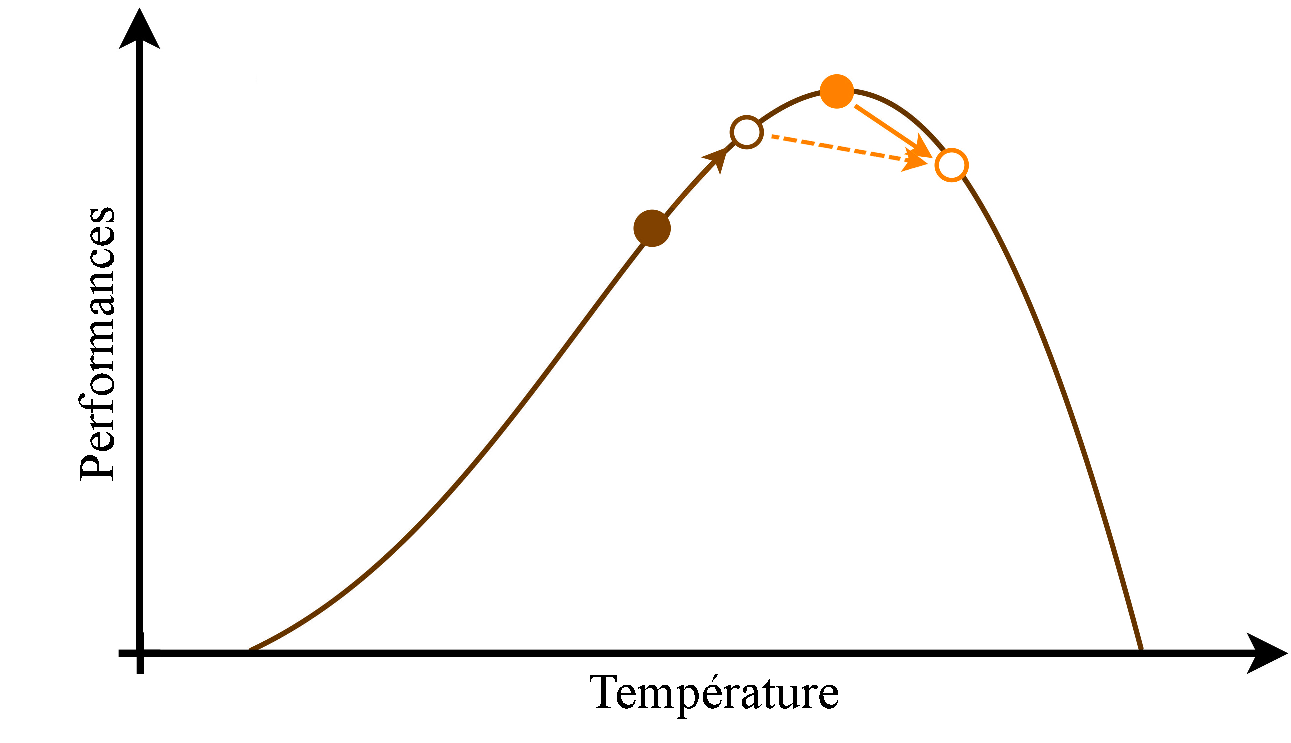
\includegraphics[width=0.66\textwidth]{1_CorpsDeThese/EA/Fig/ThermalCurve.pdf}
\caption[\lofimage{1_CorpsDeThese/EA/Fig/ThermalCurve.pdf}
Performance théorique en fonction de la température]{Performance théorique en
fonction de la température. D'après \textcites{ohlberger2013a}, Figure 1. Un
réchauffement du climat améliore les performances d'un individu qui vit dans
des conditions sous optimales si le changement est de petite amplitude (flèche
marron). Si l'individu est à l'optimum (point orange plein), le réchauffement
lui fait diminuer ses performances (flèche orange pleine). Si le changement est
de trop grande amplitude, les performances diminuent également (point marron
vide, flèche orange pointillée)}
\label{Fig:EA1}
\end{figure}

Cette sensibilité asymétrique à la température se répercute ensuite au niveau
de l'individu dans son ensemble, et en particulier sur son taux de croissance.
Ainsi, pour un individu vivant à une température sous-optimale, une augmentation
de température sera bénéfique alors qu'elle sera néfaste pour un individu vivant
déjà à sa température optimale. De même, si l'amplitude de l'augmentation est
trop importante, la température peut dépasser l'optimum et le réchauffement a
alors un effet néfaste . Ceci est illustré par la Figure
\ref{Fig:EA1}, d'après \textcites{ohlberger2013a}. Cependant, les individus sont
souvent capable d'adapter leur sensibilité à la température par plasticité
phénotypique. Ces réponses plastiques peuvent alors différer suivant la
fréquence et la longueur des changements de température
\autocites{angilletta2009a, huey1999a}.

Lorsque les températures subies sont contenus dans des valeurs non
extrêmes, permettant à un individu de se développer sans provoquer la diminution
du taux de croissance, la plupart des ectothermes suivent alors règle
taille--température déjà énoncée \autocite{atkinson1994a}. Ainsi, au cours du
développement, une plus forte température entraîne une augmentation du taux de
croissance mais une diminution de la taille adulte (Figure \ref{Fig:EA2}). On
observe donc une modification de la taille à un âge ou un stade donné avec la température (par
exemple la taille à maturité). Le suivi de ces modification permet de
déterminer précisément la norme de réaction à la température et la réponse d'un
organisme à son changement.

\begin{figure}[!ht] % Figure 1 
\centering
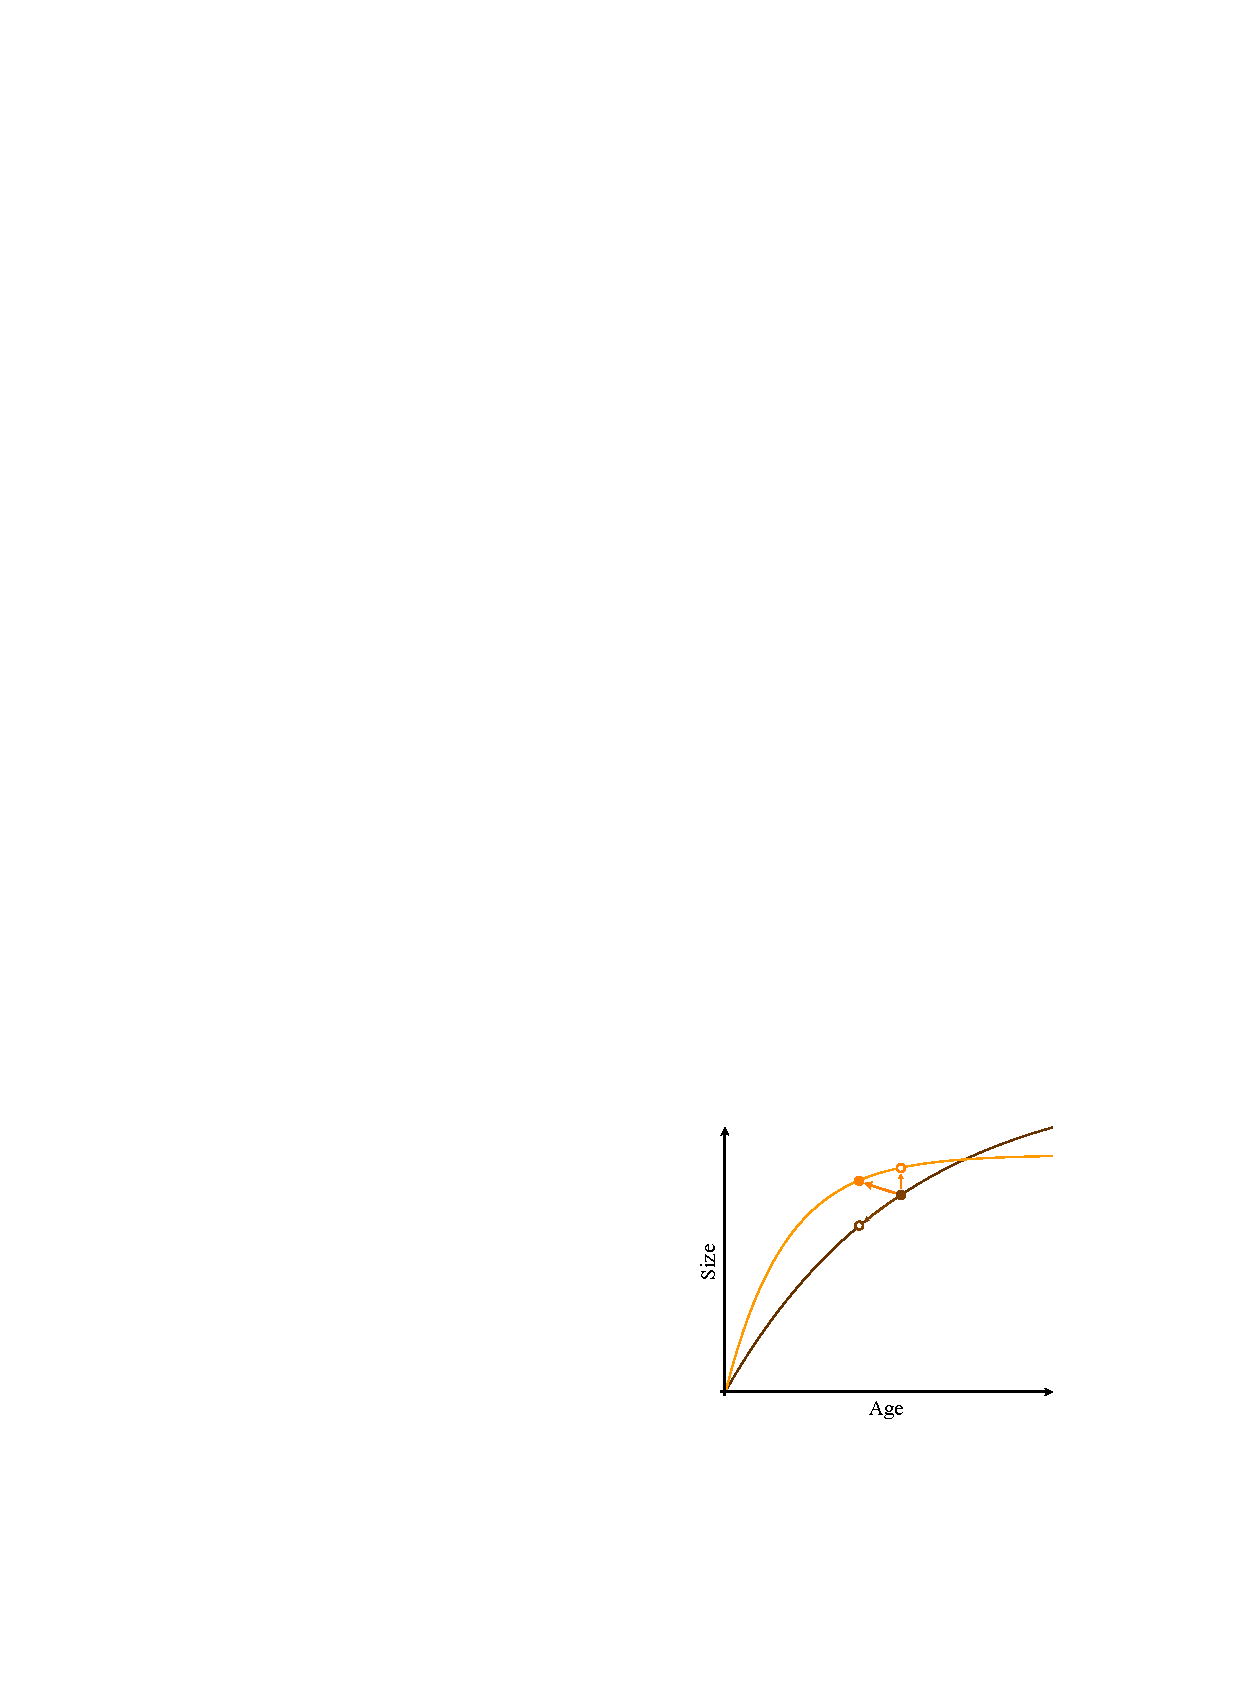
\includegraphics[width=0.5\textwidth]{1_CorpsDeThese/EA/Fig/ThermalNorm}
\caption[\lofimage{1_CorpsDeThese/EA/Fig/ThermalNorm}
Norme de réaction à la température]{Norme de réaction théorique à la
température \autocites[Figure 2]{ohlberger2013a}. Lors d'un changement de
température, le changement de taille à un âge donné (point orange plein) dépend
de l'importance relative de l'accélération de la croissance corporelle (point
orange vide), et de l'accélération du développement (point marron vide).}
\label{Fig:EA2}
\end{figure}

\subsection{Température et dynamique des populations}

La taille corporelle des individus et sa distribution étant un élément essentiel
dans la dynamique des populations, les variations de taille corporelle avec la
température ont des conséquences sur les dynamiques des populations et des
communautés. 

En effet, la température de l'environnement peut provoquer un changement de la
taille moyenne et de la structure d'une population. On retient en particulier
deux changements possibles : (i) la diminution de la taille à un âge donné avec
l'augmentation de la température (``size-at-age shift'') ; et (ii) le
changement de l'abondance relative des différents stades ou âges présents dans
la population (``structure shift''). Ces changements de structures sont causés
par l'intermédiaire de la croissance densité-dépendante, de la survie
taille-dépendante, de la compétition asymétrique entre les différentes
classes de taille et de la prédation taille-spécifique. Ces changements de
structures au niveau population peuvent ensuite se répercuter au niveau de la
communauté en affectant l'abondance relative de ses différentes espèces et son
organisation trophique. 

De plus, la température interagit fortement avec les mécanismes de densité
dépendance. Ainsi, il a par exemple été montré que le taux de croissance d'une
population peut augmenter avec la température si la population est présente en
faible densité, et à l'inverse diminuer avec la température si la population est
trop dense \autocites[chez le saumon royal][]{crozier2010a}. Dans le même
ordre d'idées, l'étude des registres de pêche du saumon d'atlantique a montré
qu'une température plus chaude était associée à des individus de grande taille si la
densité de la population était faible et l'inverse en climat froid
\autocites{huusko2012a}. 

La densité dépendance étant notamment lié à la compétition pour l'accès aux
ressources, qui elle-même dépend de la taille corporelle, l'augmentation de la
température peut provoquer une diminution de la taille moyenne dans une
population en favorisant des individus plus petits, plus compétitifs dans la
gestion de l'énergie s'il y a peu d'interférence
\autocites{persson1998a,ohlberger2012a}. Si la compétition par interférence est
forte, et une grande taille corporelle fourni un avantage compétitif conséquent,
l'effet de la température sur la compétition devient alors plus difficile à
prédire.

Enfin, la température peut avoir des effets différentiels suivant le stade ou
l'âge des individus. En effet, il a été suggéré que des individus juvéniles
survivent plus facilement à un réchauffement que des individus plus grands ou
plus vieux \autocites{peck2009a}. Une élévation de la température a donc des
effets différents suivant l'âge, le stade et la taille des individus, ce qui se
répercute sur la distribution de la taille dans la population, impactant
fortement sa dynamique. Ces changement de dynamique d'une population se
répercutent alors en cascade sur les communautés dont elles font partie, avec
des issues encore difficiles à prévoir. 


\section{Problématiques}	

\chapter{Le collembole, un modèle d'étude en écologie}
\section{Biologie}
\section{Cycle de vie}
\section{Conditions d’élevage}
\section{Méthodes de mesures et comptage (phenotypage populationnel haut débit)}
\section{Méthode de représentation graphique}


\selectlanguage{french}
\partimage[width=\textwidth]{FigParts/writing2}
\part{Résumé des travaux de thèse}


%% Chaque section est un résumé en français d'un papier présent dans les annexes.

\chapter{Accès à la ressource taille dépendant et compétition par interférence :
Analyse de séries temporelles longues de populations de collemboles \textit{Folsomia candida}}
\chaptermark{Analyse de séries temporelles structurées}
\label{chap:sp}

\vspace{5cm}

\lettrine[lines=3]{A}{ujourd'hui}, les conséquences de la compétition par
interférence sur les populations physiologiquement structurées, et plus
particulièrement les populations structurées en taille, restent assez peu
explorées. Nous présenterons dans ce chapitre les résultats d'une étude
expérimentale au cours de la quelle nous avons suivi 28 populations de
collemboles \textit{Folsomia candida} pendant $800$ à $1200$ jours. Cette étude
nous a permis d'en apprendre d'avantage sur le rôle que joue la structure des
populations à un instant donné sur la détermination de sa dynamique. Durant
cette étude, nous avons dénombré et mesuré la structure détaillée de $12$
populations du clone TO et $16$ populations du clone HA. Nous avons ensuite
réalisé une analyse qualitative et quantitative des séries temporelles obtenues
afin de relier les états (les structures) passés et présents de chaque
population avec sa dynamique future.
En particulier, cette étude nous a permis de mieux comprendre le rôle essentiel
que joue la présence d'individus de grande taille dans la régulation de la
dynamique des populations et de leur structure.

Les travaux présentés dans ce chapitre sont en cours d'écriture pour
publication, et peuvent être retrouvés dans l'Annexe \ref{Ann:SP}.

\section{Éléments de méthodologie}

\subsection{Conditions d'élevage et mesures des populations}

Nous avons élevé 28 populations de deux clones de
collemboles \textit{Folsomia candida} dans les conditions décrites dans le
Chapitre \ref{chap:method}: $12$ populations du clone TO et $16$
populations du clone HA. Pour chaque population les mesures de nombre
d'individus et de structure en taille des populations ont été réalisées toutes
les unes à deux semaines en suivant la méthode automatisée décrite dans le
Chapitre \ref{chap:method}, Section \ref{sec:bpsensor}.

\subsection{Analyse qualitative des séries temporelles}

Nous nous sommes d'abord intéressés aux dynamiques sur le long
terme de la structure des populations. Nous avons étudié de manière
qualitative ces dynamiques en traçant les séries temporelles structurées sur des
diagrammes structure-temps afin de faire ressortir le maximum d'information sur
la dynamique de la structure.
Nous avons alors séparé notre analyse en deux temps.

\subsubsection{Etat de la population}

Dans un premier temps, nous avons regardé la structure en taille des populations
de manière globale afin de repérer les structures caractéristiques que l'on
pouvait observer, sans considérer les dynamiques de court terme. Nous décrivons
alors plusieurs structures typiques différentes suivant le clone considéré et le
niveau de densité de la population.

\subsubsection{Dynamique de la structure de la population}

Dans un second temps, nous nous sommes attachés à décrire les dynamiques
temporaires que l'on peut observer sur les diagrammes structure-temps. Nous
avons essayé de déterminer des motifs dynamiques que l'on pouvait rattacher à
certains types de structures de populations, telles que celles décrites au
par avant, ou à certains changements dans ces structures.

\subsection{Analyse quantitative des dynamique de populations}

Suite à la description qualitative des dynamiques, nous avons réalisé une
analyse quantitative des structures observées et de leur dynamique. 

\subsubsection{Analyse en composante principale}

A chaque date de mesure, les données comprennent le nombre d'individus et pour
chaque individu sa longueur corporelle. Nous avons regroupé les données de
l'ensemble des populations à toutes les dates de mesures et nous avons
discrétisé la taille en classes de $0.1mm$ de $0$ à $3mm$. Nous obtenons ainsi
un tableau de données de $3341$ lignes (une ligne par classe de taille par date
par population) et $30$ colonnes. Chacune des colonne peut alors être considéré
comme un vecteurs de base dans l'espace à $30$ dimensions qui constitue l'espace
des structures de nos populations, et chaque ligne comme une observation dans
cet espace. Étant donnée la différence d'ordre de grandeur dans les nombres
d'individus entre juvéniles et adultes, nous avons utilisé le logarithme des
nombre d'individus dans chacune des classes de taille.

En considérant que chaque ligne est indépendante des autres, nous avons alors
réalisé une analyse en composantes principales (ACP) de nos données compilées.
Cela nous a permis d'extraire les quelques premières composantes et les vecteurs
et valeurs propres correspondantes. Ainsi, en ne conservant que peu de
composantes, on obtient une représentation condensée à quelques dimensions
(deux ou trois dans notre cas) des données de départ. Nous avons alors projeté
chacune des dynamiques de la structure des populations sur les deux première
composantes de la décomposition. Un point dans l'espace à deux dimension
représente alors une condensation de la structure d'une population à une date
donnée. 

\subsubsection{Regroupement non hiérarchique et projection sur les premières
composantes}

Parallèlement à l'ACP, nous avons effectué un regroupement non hiérarchique par
l'algorithme des ``k-means'' de nos données compilées. Ceci permet de regrouper
ensemble les structures de populations qui partagent des caractéristiques
communes, indépendemment de la date de mesure, du clone ou de la dynamique de la
population. Ainsi, nous avons pu déterminer quatre groupes cohérents de
structures de populations et identifier leur caractéristiques précises. Une fois
projetés sur les deux premières composantes de l'ACP, les groupes obtenus
délimentent quatre régions distinctes du plans, confirmant ainsi la cohérence du
regroupement. 
 
\subsubsection{Dynamique des populations}

La visualisation des données sur le plan des deux premières composantes de l'ACP
et le regroupement en quatre types de structures permettent de représenter la
dynamique de la structure des populations comme une trajectoire dans ce plan.
Cette trajectoire permet alors une analyse objective des dynamiques en
déterminant par exemple des temps de résidence dans chacune des structures type,
les nombres de transitions entre différentes structures types et la direction de
ces transitions. 

\section{Résultats}

Nous présenterons ici l'analyse détaillée de quatre populations, deux du clone
TO et deux du clone HA, ainsi que les résultats de l'analyse de l'ensemble des
populations. L'analyse graphique de chacune des populations est disponible à la
fin de l'article en Annexe \ref{Ann:SP} page \pageref{Ann:SP}. 

\subsection{Etude descriptive}

\subsubsection{Etats des populations}

La première partie de cette étude concerne une description qualitative des
périodes stables de la structure des populations (Figure \ref{fig:SP1}). On
appellera état des populations ces structures caractéristiques que l'on retrouve dans les
différentes populations. 

\begin{figure}[!ht]
\begin{center}
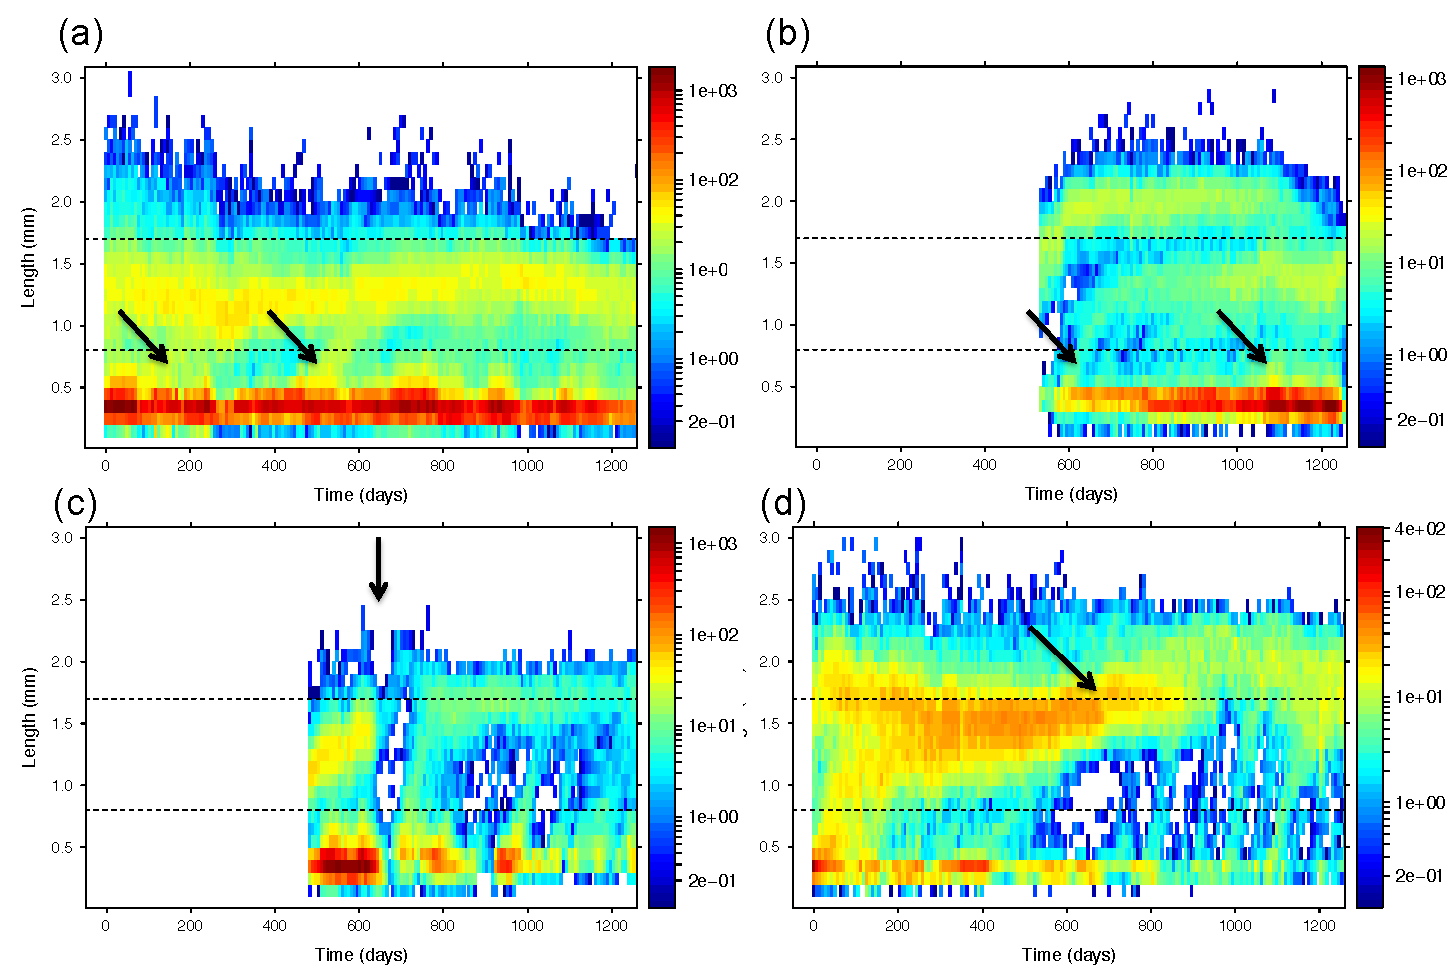
\includegraphics[width=0.95\textwidth]{1_CorpsDeThese/Resumes/Fig/SP01}
\caption[\lofimage{1_CorpsDeThese/Resumes/Fig/SP01}Dynamiques de la
structure de 4 populations]{Dynamique de la structure de 4 populations de
collembole. (a) Clone TO, réplicat 3. (b) Clone HA, réplicat 15. (c) Clone TO,
replicat 11. (d) Clone HA, réplicat 4. Les flèches noires en (a) et (b) montrent
des périodes de recrutement. Les flèches noires de (c) et (d) montrent des
événements conduisant à un nouveau recrutement, respectivement une catastrophe
(c) et la sénescence de la cohorte d'adultes (d).}
\label{fig:SP1}
\end{center}
\end{figure}

Les Figures \ref{fig:SP1}a et b montrent deux populations aux structures
relativement stables, mais dont la distribution en taille diffère. Dans le
premier cas, on constate que la distribution de la taille est fortement
bi-modale avec un groupe de juvéniles très dense ($>700$ individus de moins de
$0.5mm$) et un groupe de d'adultes ($<250$ individus de plus de $0.8mm$), mais
très peu d'individus de taille intermédiaire. Dans le second cas, on retrouve
ces deux même groupes pendant la totalité de la série temporelle, mais avec une
longue période pendant la quelle un troisième groupe de très grands adultes
subsiste ($>1.2mm$). Ces distributions multi-modales sont universelles dans les
populations étudiées. La plupart des populations ont une structure bi-modale,
plus ou moins stable dans le temps, tandis que certaines populations montrent
une structure tri-modale, exclusivement chez le clone HA. Le clone HA est donc
cable de produire des adultes de très grand taille à la survie très longue, ce
que TO est incapable de faire.

\subsubsection{Dynamique de la structure}

Dans un second temps, on s'intéresse maintenant aux événements dynamiques rapide
à l'échelle des séries temporelles. En effet, même si la structure peut être
relativement stable (Figure \ref{fig:SP1}a et b), on peut observer que des
processus dynamiques sont à l'oeuvre.
 
\paragraph{Recrutement de cohortes}

Un premier processus remarquable est le recrutement de juvéniles dans les
classes d'adultes (flèches sur les Figures \ref{fig:SP1}a et b). Ces périodes de
recrutement  durent entre quelques dizaines et quelques centaines de jours, et
se retrouve plus ou moins fréquemment, mais dans l'ensemble des populations
étudiées. On constate sur la Figure \ref{fig:SP1}b que ces recrutements
n'atteignent jamais la cohorte d'adultes les plus grands.
Ceci est vrai pour toutes les populations dans les quelles un groupe d'adultes
de très grande taille subsiste. Lorsque ces individus géants sont présents dans
une populations, il semble alors impossible pour les autres de grandir jusqu'à
ces tailles.

Ces périodes de recrutement permettent également d'estimer des taux de
croissance corporelle en fonction des conditions de la population (clone et
densité dans les différentes classes) en mesurant la pente de la cohorte qui
recrute. Ainsi, le taux de croissance de la cohorte marquée par la seconde
flèche de la Figure \ref{fig:SP1}a est d'environ $5\cdot 10^{-3}mm/j$, soit
$1mm$ tous les 200 jours. L'étude de ces taux de croissance en fonction de la
densité et des conditions de température fera l'objet du Chapitre \ref{chap:fip}
et de l'Annexe \ref{Ann:fip}.

Ces périodes de recrutement surviennent parfois à la suite d'événement
catastrophiques. On constate sur la Figure \ref{fig:SP1}c (flèche) que c'est
après la disparition brutale et quasi-totale des adultes que survient un des
plus gros recrutements d'individus de la série temporelle. Ceci se retrouve
également sur d'autre population (voir Table \ref{tab:SP}). Ainsi, la
disparition brutale des adultes de la population déclenche le recrutement de
nouveaux individus chez les adultes. 

Enfin, le recrutement de nouvelle cohortes de juvéniles peut également
intervenir après le déclin naturel du groupe d'adultes, soit chez le groupe de
géants (Figure \ref{fig:SP1}b, seconde flèche), soit le seul groupe présent
(Figure \ref{fig:SP1}d, flèche). On constate par exemple dans le second cas que
pendant une très longue période la population est composée de quelques jeunes et
d'une très large cohorte d'adulte, avec très peu de recrutement de nouveaux
adultes. Ce groupe d'adulte décline au cours du temps, et lorsqu'il a
suffisamment diminué en densité (aux environs de $800$ jours, flèche), des
recrutements de jeunes commencent à survenir. Ceci confirme le rôle des
adultes de plus grande taille dans le contrôle de la dynamique de la structure
et le renouvellement des populations. 

\paragraph{Plasticité de la taille adulte}

L'étude de ces séries temporelles révèle également des ajustements de la taille
des adultes au cours des différents événements décrits précédemment. Tout
d'abord, suivant les conditions démographiques, les cohortes d'adultes se
stabilisent à différentes tailles. Les populations montrées en exemple sur la
Figure \ref{fig:SP1} montrent chacune une taille d'équilibre différente. En
particulier, la taille adulte a tendance à être plus grande quand la densité
de la population est plus faible. Ce point fera également l'objet d'une étude
approfondie dans le Chapitre \ref{chap:fip}.

De plus, les individus sont capables d'ajuster rapidement leur taille corporelle
en fonction des changements de conditions environnementales et démographiques.
Après la chute catastrophique de la cohorte d'adulte montrée Figure
\ref{fig:SP1}c, les adultes survivants reprennent une croissance très rapide sur
une courte durée (augmentation de près de $40\%$ de leur taille corporelle en
quelques semaines).
De même dans le cas de la sénescence des adultes (Figure \ref{fig:SP1}d), où les
adultes restant grandissent de $1.7mm$ à près de $2.2mm$.

De façon plus étonnante, les adultes sont également capables de diminuer leur
taille corporelle. Par exemple au cours des $200$ premiers jours sur la Figure
\ref{fig:SP1}d où la taille des adultes diminue pendant qu'une grande cohorte de
juvéniles atteint la maturité. Ces rétrécissements des adultes ont été observées
dans d'autres populations (HA réplicats 1 à 3, TO réplicats 5 et 9 par exemple).
La plasticité de la taille adulte des collemboles est décrite et étudiée par
\textcites{mallard2013b} dans ses travaux de thèse.

La Table \ref{tab:SP} résume les dates où les différents événements décrits ont
été observés dans les populations étudiées. 

{\tiny
\begin{longtable}{
	p{\dimexpr.12\linewidth-2\tabcolsep-1.3333\arrayrulewidth}% column 1
 	p{\dimexpr.128\linewidth-2\tabcolsep-1.3333\arrayrulewidth}
 	p{\dimexpr.128\linewidth-2\tabcolsep-1.3333\arrayrulewidth}% column 1
 	p{\dimexpr.128\linewidth-2\tabcolsep-1.3333\arrayrulewidth}
 	p{\dimexpr.12\linewidth-2\tabcolsep-1.3333\arrayrulewidth}% column 1
 	p{\dimexpr.12\linewidth-2\tabcolsep-1.3333\arrayrulewidth}
 	p{\dimexpr.126\linewidth-2\tabcolsep-1.3333\arrayrulewidth}% column 1
 	p{\dimexpr.126\linewidth-2\tabcolsep-1.3333\arrayrulewidth}}
 	
 	\caption{Dates d'observations des états et dynamiques
 	décrites. Les nombres correspondent aux dates en jours ou aux
 	intervalles pendant les quels les événements ont été
 	observés.}\label{tab:SP}\\
 	\hline
 	\endhead
 	
\hline
\endfoot

Populations & Structure Trimodale & Longue période sans recrutement &
Recrutement fréquent & Evénement catastrophique & Senescence de la cohorte adulte &
Croissance adulte d'ajustement & Rétrécissement adulte d'ajustement \\
\hline\\
HA r1 & - 			& - 		& - 		& - 	& 500  & 500-650  & 650-750  \\
HA r2 & - 			& - 		& - 		& - 	& 800  & 650-900  & - 		 \\
HA r3 & - 			& - 		& - 		& - 	& 800  & 900-1000 & 1000-1250\\
HA r4 & - 			& - 		& - 		& - 	& 800  & 600-1000 & -        \\
HA r5 & 600-1000 	& - 		& - 		& - 	& 1000 & - 		  & - \\
HA r6 & - 			& 800-1250 	& - 		& - 	& -    & - 		  & - \\
HA r7 & 700-1100 	& - 		& - 		& - 	& 1000 & - 		  & - \\
HA r8 & 600-1000 	& - 		& - 		& - 	& 950  & - 		  & - \\
HA r9 & 700-1200 	& 700-1100 	& - 		& - 	& -    & - 		  & - \\
HA 10 & 600-900 	& - 		& - 		& - 	& 900  & - 		  & - \\
HA 11 & 600-1100 	& 700-1250 	& - 		& - 	& 1100 & - 		  & - \\
HA 12 & 600-900 	& - 		& 600-1250 	& - 	& 1000 & - 		  & - \\
HA 13 & 600-1100 	& - 		& 600-1250 	& - 	& 1100 & - 		  & - \\
HA 14 & 600-1100 	& 600-1000 	& - 		& - 	& 1100 & - 		  & - \\
HA 15 & 600-1100 	& - 		& 600-1250 	& - 	& 1100 & - 		  & - \\
HA 16 & 600-1200 	& - 		& - 		& - 	& 1200 & - 		  & - \\
TO r1 & - 			& 400-600 	& 0-400 	& - 	& 400  & 400-600  & -\\
	  &				& 700-1000	& 1000-1250 & 		&	   &		  &\\
TO r2 & - 			& 500-750 	& 0-450 	& - 	& 400  & 500-700  & - \\
	  & 			& 			& 1000-1250 &		&	   &		  &\\
TO r3 & - 			& 600-1250 	& - 		& - 	& -    & - 		  & 0-200\\
TO r4 & - 			& - 		& 0-1250	& - 	& 400  & - 		  & 700-1000\\
TO r5 & - 			& - 		& - 		& 900 	& -    & 900-1000 & 500-700\\
TO r6 & - 			& 600-950 	& - 		& 950 	& -    & 950-1000 & -\\
TO r7 & - 			& - 		& 500-1250 	& - 	& -    & - 		  & -\\
TO r8 & - 			& 600-800 	& 800-1250 	& - 	& 1000 & 1000-1100& -\\
TO r9 & - 			& 600-1000 	& - 		& - 	& 950  & 900-1000 & 500-600\\
TO 11 & - 			& - 		& 700-1250 	& 650 	& -    & 650-750  & -\\
TO 12 & - 			& - 		& - 		& 750 	& -    & 750-850  & -\\
TO 13 & - 			& 500-800 	& 800-1250 	& 800 	& -    & - 		  & -\\

\end{longtable}
}

\subsection{Analyse quantitative des dynamiques}

\subsubsection{Composantes principales}

\begin{figure}[!ht]
\begin{center}
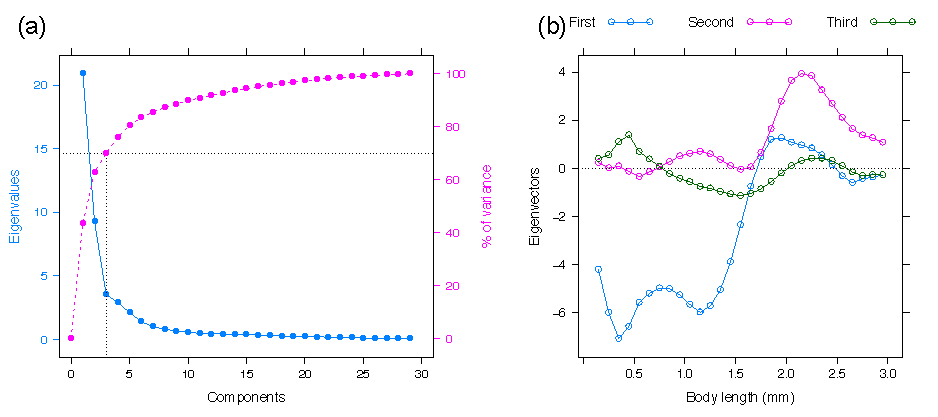
\includegraphics[width=0.95\textwidth]{1_CorpsDeThese/Resumes/Fig/SP02}
\caption[\lofimage{1_CorpsDeThese/Resumes/Fig/SP02}Composantes
principales]{(a) Scree plot de l'ACP. La ligne bleue pleine donne les valeurs
propres, la ligne pointillée donne le pourcentage cumulé de variance expliquée.
(b) Coordonnées des trois premiers vecteurs propres.}
\label{fig:SP2}
\end{center}
\end{figure}

La Figure \ref{fig:SP2}a représente les valeurs propres de l'ACP et le
pourcentage cumulé de variance expliquée. On observe une cassure nette après la
troisième composante, les trois premières composantes expliquant $70\%$ de la
variance totale. Cela montre que les trois premières composantes permettent
d'expliquer l'essentiel des variations entre les structures dans nos différentes
populations. La Figure \ref{fig:SP2}b montre que ces trois composantes
expliquent des variations sur l'ensemble de notre espace de départ sans classe
de taille non expliquée..
En particulier, la première composante expliquant $43\%$ de la variance
correspond essentiellement aux variations dans les individus de moins de
$1.5mm$. La seconde composante quand à elle, qui représente $20\%$ de la
variance explique une partie des variations des petits adultes ($0.8$ à
$1.3mm$), et principalement au niveau des individus de plus de $1.6mm$. La troisième
composante enfin permet de distinguer entre les individus de taille
intermédiaire ($0.8$ à $1.9mm$) et les petits individus ($<0.8mm$). Ces trois
composantes permettent de définir plusieurs groupes de classes de taille sans a
priori: (i) les juvéniles ($<0.6mm$), négatifs sur le premier axe et positif sur
le troisième; (ii) les petits adultes (entre $0.6$ et $1.2mm$) positif sur le
second axe, négatif sur les autres; (iii) les adultes intermédiaires ($1.2$ à
$1.9mm$) négatifs sur le troisième axe; et (iv) les grands adultes ($>1.9mm$),
positifs sur le second axe. Ces groupes recoupent bien la description
qualitative des diagrammes mais sans a priori sur les limites entre groupes.

Les deux premières composantes représentant $63\%$ de la variance, nous ne
conserveront pas la troisième composante dans la suite de l'étude. Cela nous
permettra une représentation graphique simplifiée des structures des populations
dans le plan des deux premières composantes. 

\subsubsection{Groupement non hiérarchique}

En utilisant l'algorithme des ``k-means'', nous avons regroupé les structures
qui partageaient des caractéristiques communes en quatre groupes. En traçant ces
structures ensemble, nous avons pu déterminer quatre grandes structures typiques
de populations expérimentales (Figure \ref{fig:SP3a}): (i) une
structure avec beaucoup de juvéniles et des adultes de petite taille (type $1$);
(ii) une structure avec des adultes de taille intermédiaire (type $2$); (iii)
une structure avec moins de juvéniles et des adultes de grande taille (type
$3$); et (iv) une structure trimodale avec des juvéniles, des petits et des
grands adultes (type $4$).

\begin{figure}[!ht]
\begin{center}
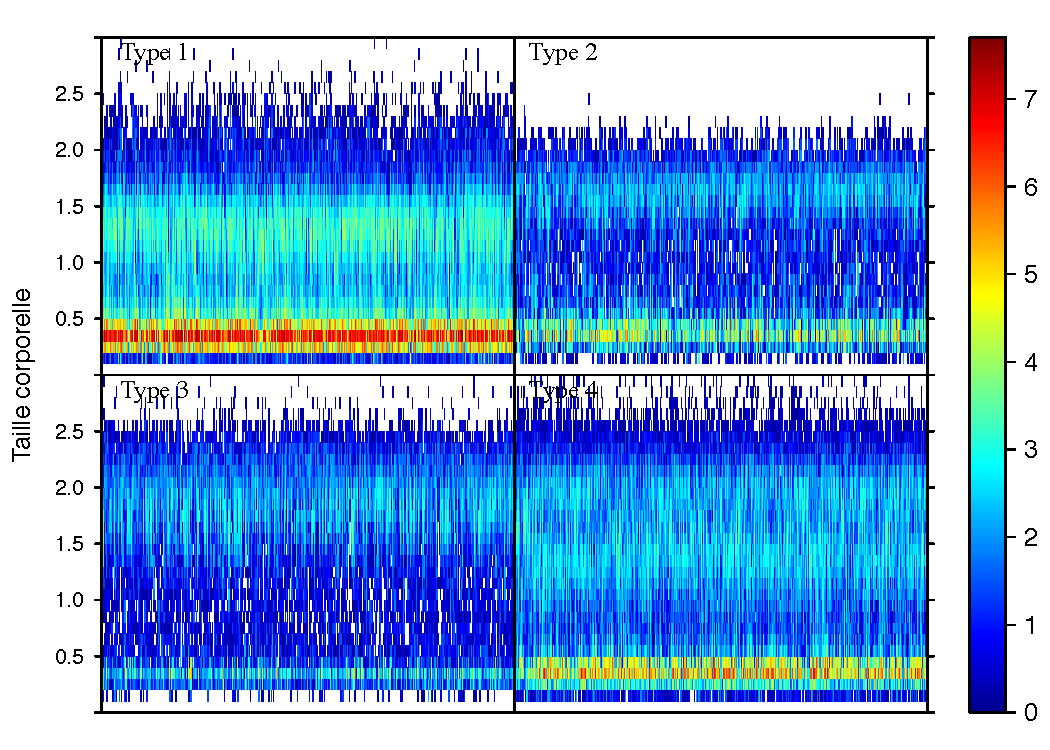
\includegraphics[width=0.95\textwidth]{1_CorpsDeThese/Resumes/Fig/SP02b}
\caption[\lofimage{1_CorpsDeThese/Resumes/Fig/SP02b}Quatres grands
types de structures]{Structures caractéristiques des quatre grands types de
structure identifiés.}
\label{fig:SP3a}
\end{center}
\end{figure}

En projetant la structure de chacune des populations à chaque date de mesure
sur les deux premières composantes de l'ACP, et en séparant les points en
fonction du type de structure auxquels ils appartiennent, on constate que la
séparation en quatre groupes reste remarquablement cohérente dans l'espace
réduit à deux dimensions (Figure \ref{fig:SP3}), et délimitent quatre régions
distinctes du plan.

\begin{figure}[!ht]
\begin{center}
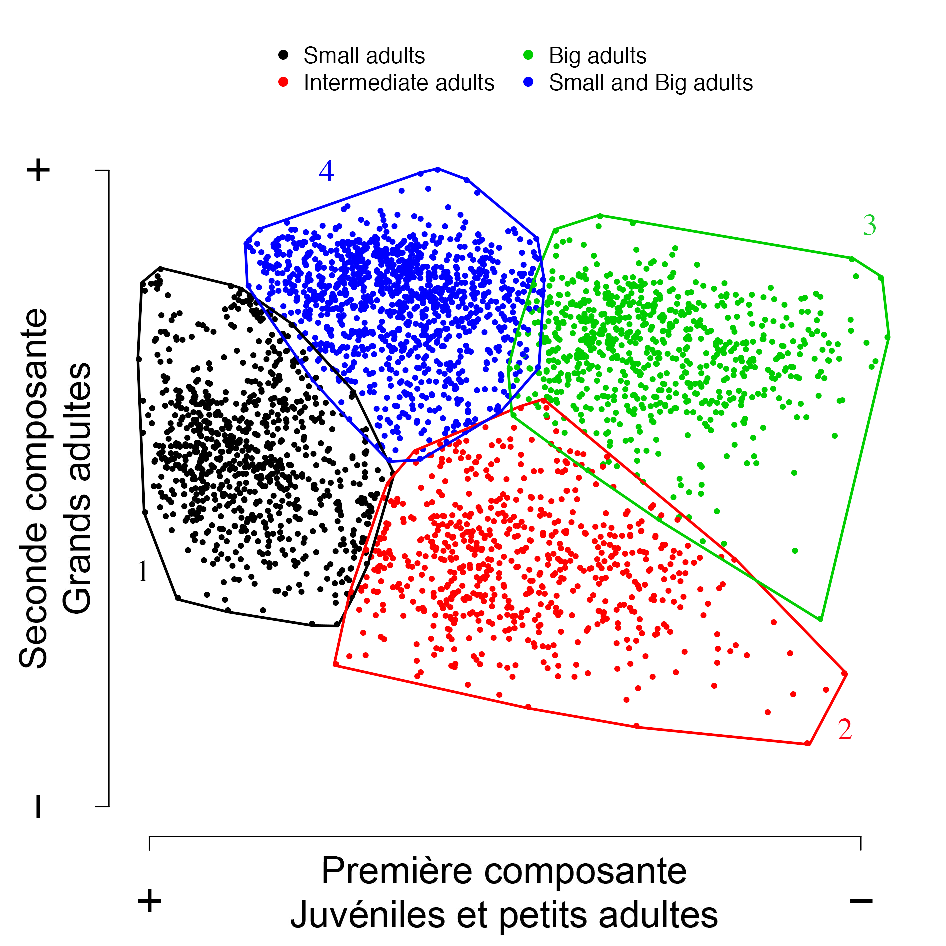
\includegraphics[width=0.75\textwidth]{1_CorpsDeThese/Resumes/Fig/SP03b}
\caption[\lofimage{1_CorpsDeThese/Resumes/Fig/SP03b}Projection des données
sur les deux premières composantes]{Projection des structures sur les deux
premières composantes de l'ACP et groupement en 4 types de structure. Les
domaines délimités seront reportés sur les trajectoires temporelles dans le
plan des deux premières composantes.}
\label{fig:SP3}
\end{center}
\end{figure}

Cette représentation permet une classification objective de la structure d'une
population à un temps donné dans un des quatre type de structure, ainsi que
d'observer la trajectoire temporelle dans le plan des deux premières composantes
de l'ACP et donc sa dynamique entre les différentes structures caractéristiques. 

\subsubsection{Trajectoires dans le plan des composantes}

\begin{figure}[!ht]
\begin{center}
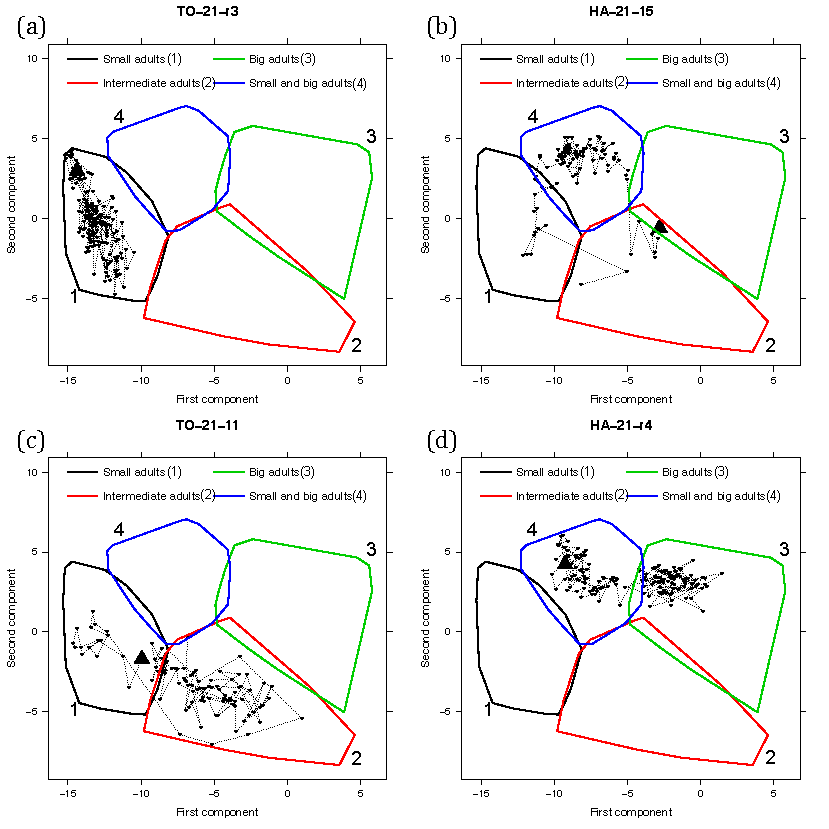
\includegraphics[width=0.95\textwidth]{1_CorpsDeThese/Resumes/Fig/SP04}
\caption[\lofimage{1_CorpsDeThese/Resumes/Fig/SP04}Trajectoires des
popualtions exemple dans le plan des composantes]{Trajectoires des
populations exemples dans le plan des composantes. Les lignes colorées et
numérotées représentes les quatre grands types de structure issus de la
classification non hiérarchique. Chaque points est une mesure de structure à
une date donnée. Le triangle représente le début de la trajectoire. Les lignes
pointillées relient chronologiquement les points.}
\label{fig:SP4}
\end{center}
\end{figure}

La Figure \ref{fig:SP4} montre les mêmes populations que sur les diagrammes
structure-temps de la Figure \ref{fig:SP1}, en projetant les structures dans le
plan des deux premières composantes. Cette représentation permet de confirmer
numériquement que la population TO 3 (Figures \ref{fig:SP1}a et \ref{fig:SP4}a)
reste tout le temps dans une structure de type 1 alors que la population TO 11
(Figures \ref{fig:SP1}c et \ref{fig:SP4}c) débute dans une structure de type 1
mais converge finalement vers une structure de type 2 avec moins de juvéniles et
des adultes plus grands. De même pour les populations HA  (Figures
\ref{fig:SP1}bd et \ref{fig:SP4}bd) qui restent toutes les deux dans une
configuration de type 4 trimodale avant de basculer, l'une vers une structure de
type 2 avec des adultes petits à intermédiaires (panels b), l'autre vers une
structure de type 3 avec des grands adultes (panels d).

\subsubsection{Stabilité des structures et transitions}

L'ACP et la projection des dynamiques sur les deux premières composantes
permettent de mesurer des temps de résidence dans chacun des 4 types de
structure, et des transitions entre les grands types. Par exemple, alors que la
population TO 3 (Figures \ref{fig:SP1}a et \ref{fig:SP4}a) est très stable et
passe 1200 jours dans le même type de structure, les autres populations ont
tendance avoir des transitions entre plusieurs types de structures. En
particulier, la population HA 15 (panels b) a une phase transitoire d'une
cinquantaine de jours en type 2 avant de se stabiliser en type 4 pendant 550
jours, puis de revenir en type 2. En conduisant la même analyse sur chacune des
28 populations, nous pouvons alors étudier la distribution du temps passé dans
chacune des régions par chacun des clones. 

\begin{figure}[!ht]
\begin{center}
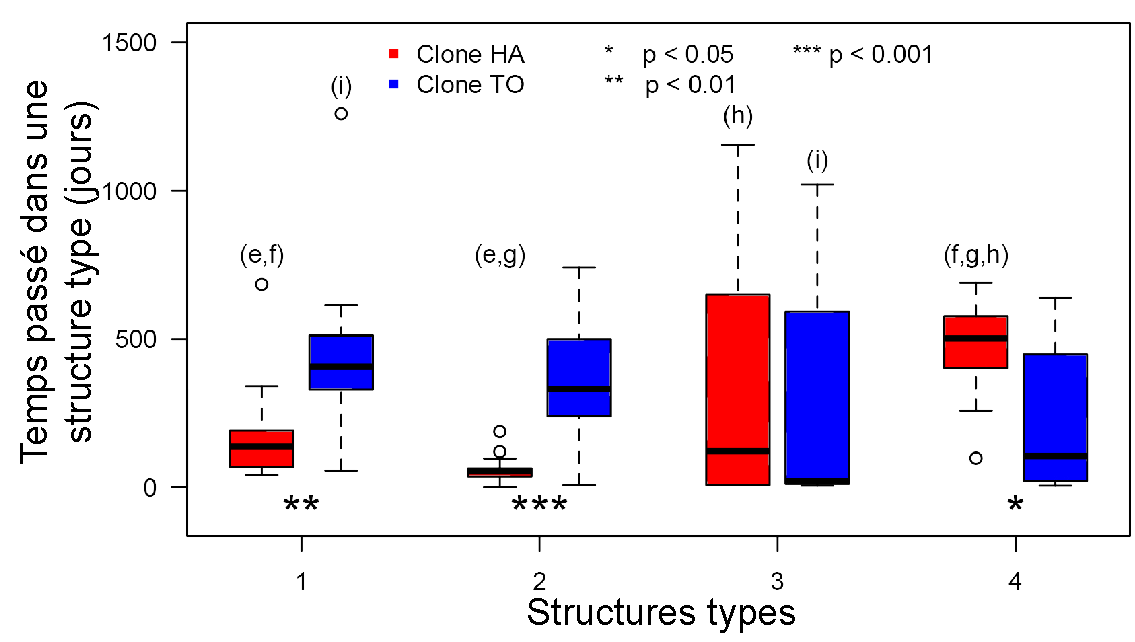
\includegraphics[width=0.95\textwidth]{1_CorpsDeThese/Resumes/Fig/SP05}
\caption[\lofimage{1_CorpsDeThese/Resumes/Fig/SP05}Temps de
résidence dans les structures types]{Temps passé dans chacun des types de
structure caractéristique suivant les clones. Les lettres montrent les
différences significatives dans les distributions (Tests de Kolmogorov-Smirnov
à deux échantillons: (e) D=0.54, p=0.02, (f) D=0.78, p=0.0003, (g) D=0.93,
p=3x10-6, (h) D=0.53, p=0.03, (i) D=0.67, p=0.04). Les étoiles montrent les
différences significatives entre clones dans un même type de structure.}
\label{fig:SP5}
\end{center}
\end{figure}

On constate alors que les différents types de structures ne sont pas tous aussi
stables (Figure \ref{fig:SP5}). Ainsi, bien que la variabilité soit très grande,
les temps de résidence les plus longs observés sont dans le type 3, avec des
adultes de grande taille.
Ces adultes de grande taille ont une très grande longévité et subissent peu de
compétition de la part des autres individus, ce qui a un effet stabilisant sur
la structure de la population. Cet effet est également visible pour les
structures trimodales (type 4) ou les temps de résidences sont également très
long. A l'opposé, les structures de types 2 sont les moins stables, en effet,
les adultes intermédiaires vont être soit exclus compétitivement par les plus
petits, ce qui fait revenir la population en type 1, soit plus fréquemment
continuer à grandir, ce qui fait basculer la population en type 3.

On constate également qu'il existe des différence marquées entre clones. Ainsi,
TO passe plus de temps dans les structures de type 1 et 2 où les adultes sont
plus petits et la densité de juvéniles est importante, alors que HA est plus
souvent dans une structure de type 3 ou 4 avec des adultes de très grande taille
et moins de juvéniles. Cela reflète des stratégies d'histoire de vie différentes
des clones TO et HA, le premier ayant tendance à privilégier la reproduction sur
la croissance, alors que le second privilégie la croissance sur la reproduction.

\section{Discussion}

\subsection{Conséquences des différences génétiques sur la dynamique des
populations}

Les différences de stratégies d'histoires de vie peuvent avoir un effet très
fort sur la dynamique des populations via notamment deux impactes. Le premier
est sur la réponse à la compétition, en effet les juvéniles sont plus compétitif
dans le cas de l'exploitation alors que les grands adultes sont supérieurs dans
le cas de l'interférence. Le second concerne la réponse à des changements de
températures puisqu'on a vu que ces derniers pouvaient affecter la taille
individuelle et les structures des populations. Les deux clones étudiés sont
connus pour leur stratégies différentes \autocites{tully2006a,tully2008a}, TO
étant très flexible dans son investissement reproducteur au détriment de sa
taille corporelle, alors que HA l'est moins mais atteint des plus
grandes tailles.

Ces différences affectent la dynamique de la structure des populations puisque
la faible flexibilité de HA et sa capacité à produire des adultes de grande
taille lui permettent d'atteindre des structures de type 3 voir 4 très
stables alors que TO reste dans des structures de type 1 ou 2. Une
fois établis, les adultes de grande taille dominent la population et empêchent
les autres individus de grandir monopolisant la ressource, ce qui amène
notamment à la stabilisation d'un groupe de petits adultes et des structures de
type 4 trimodales. Cela montre l'importance de connaître les stratégies
d'histoire de vie des espèces étudiées afin de comprendre correctement la
dynamique de leur structure et \textit{in fine} de prédire la dynamique de la
population dans son ensemble.

\subsubsection{Le rôle des conditions initiales}

Bien que la structure de type 4 semble très stable, il est intéressant de noter
qu'elle n'est visible qu'au début de certaines séries temporelles. En effet, ce
type de structure est très stable localement, mais n'est atteignable que dans
des conditions très particulières. Il est nécessaire: (i) que les individus
puissent grandir vite jusqu'à des très grandes tailles, ce qui est le cas
de HA mais pas de TO; et (ii) que le niveau de compétition soit à son minimum,
ce qui se traduit par une absence d'adulte dans la population, et une faible
densité de jeunes. Dans ces conditions, les jeunes présents vont alors grandir
jusqu'aux plus grandes tailles et commencer à se reproduire tout en monopolisant
la ressource, ce qui n'autorise les autres juvéniles à grandir que jusqu'à des
tailles intermédiaires. 

Les autres types de structures dépendent aussi des conditions initiales. Une
forte densité de juvéniles comme condition initiale d'une population conduira à
une structure de type 1 alors qu'une distribution relativement homogène en
densité moyenne conduira à une structure de type 2 chez TO et de type 3 chez HA.
L'importance des conditions initiales montre la coexistence des quatre
attracteurs quasi-stables de la structure des populations. De plus, les
transitions entre ces attracteurs sont généralement dues soit à un événement
catastrophique, soit à la sénescence des adultes de grande taille. 

Enfin, cette sensibilité aux conditions initiales montre l'importance de
considérer la structure dans l'étude de la dynamique des populations. En effet,
bien que le nombre d'individus globale puisse être le même, une structure
différente pourra mener à des dynamiques très différentes, ce
qui inclue la survie potentielle de la population. Cela va dans le sens des
résultats de \textcites{benton2005a} sur la dynamique de populations
d'acariens structurées en âge montrant que des séquences données de changements
environnementaux peuvent amener à des dynamiques très différentes en fonction de
détails des conditions initiales de la structure en âge et de la densité des
populations.

\subsubsection{La compétition par interférence}

Nous avons montré à plusieurs reprise le rôle déterminant que jouent les adultes
de grande taille dans la dynamique de nos populations. Si l'accès à la ressource
n'était régulé que par la compétition par exploitation, tous les individus
parviendraient à accéder à la ressource, et la théorie du budget énergétique
dynamique nous prédit que les grands individus seraient exclus par les plus
petits, plus efficaces dans leur gestion de l'énergie. Dans ces conditions, les
structures tendraient vers une majorité de juvéniles et des adultes qui ne
grandissent plus une fois la maturité atteinte. 

Or, nos dynamiques montrent clairement que les individus de grande taille
exercent une domination sur les populations: (i) certaines conditions permettent
l'émergence et le maintient à long terme de cohortes d'adultes géants; (ii) lors
de la disparition catastrophique d'une cohorte d'adultes, les juvéniles présents
commencent immédiatement à grandir; (iii) la sénescence d'une cohorte d'adulte
et sa disparition progressive se traduit aussi par une reprise de la croissance
des juvéniles; et (iv) des cohortes très dense d'adultes s'accompagnent
généralement de longues périodes sans recrutement. Ainsi, il semble que nos
populations soient régulées par la domination des adultes. Un mécanisme probable
permettant cette domination adulte serait la position privilégiée qu'ils
occupent dans l'accès à la ressource disponible, privant les plus petits
individus, les empêchant de grandir. Ceci est un mécanisme caractéristique de la
compétition par interférence. Lorsque le nombre d'adultes de grande taille
diminue, la pression de compétition est relâchée et les plus petits individus
parviennent de nouveau à accéder à la ressource et à se développer.


\section{En conclusion}

Cette étude montre ainsi que l'analyse de la dynamique temporelle de la
structure des populations permet d'accéder plus précisément aux mécanismes en
jeu dans leur régulation, tels que le rôle des stratégies individuelles
d'histoire de vie, ou le type d'interaction compétitive à l'oeuvre. Nous pensons
que cette étude est un exemple concret du fait qu'une population puisse être
contrôlée par ses adultes les plus grands, donnant lieu à des dynamiques
complexes qui dépendent directement des stratégies d'histoire de vie des
individus et des conditions environnementales, y compris la densité de
la population.
Modéliser le rôle de la compétition par interférence dans la dynamique des populations structurées, dans le cadre des modèles PSP, nous
permettra de confirmer son rôle essentiel dans la survie des
individus de grande taille, et dans l'émergence de dynamiques temporelles
impliquant des distributions de taille multi-modales (Chapitre
\ref{chap:amnat}).

De plus, il serait nécessaire de vérifier précisément le rôle joué par les
adultes, notamment pour confirmer leur domination dans l'accès aux ressources,
ce qui viendrait confirmer l'hypothèse de l'interférence comme mécanisme de
régulation des populations. Ceci fera l'objet d'une étude expérimentale
présentée dans le Chapitre \ref{chap:sm}.




\chapter[Interférence vs. exploitation et dynamique des populations
structurées][Interférence et populations structurées]{Interférence vs.
exploitation et dynamique des populations structurées}
\label{chap:amnat}

\vspace{2cm}
\begin{Spacing}{1}
\texttt{
Le Bourlot, Vincent, Thomas Tully and David Claessen, "Interference versus
Exploitative Competition in the regulation of Size-Structured Populations"\\
under review at The American Naturalist
}
\end{Spacing}
\vspace{2cm}


\lettrine[lines=3]{D}{ans le chapitre} précédent, nous avons pu voir le rôle
prépondérant que jouent les individus de grande taille dans la régulation des
populations de collembole \textit{Folsomia candida} élevées en laboratoire. Les
individus de grande taille impactent fortement la population par l'intermédiaire
des interactions entre individus et de la compétition pour les ressources. La
compétition est un des facteurs principaux dans la régulation de la dynamique
des populations et des communautés. Son effet peut être soit direct entre
plusieurs individus via la compétition par interférence, ou par l'intermédiaire
de la ressource dans la compétition par exploitation.

L'impact de la compétition par exploitation sur la dynamique des populations a
déjà été largement étudié, tant d'un point de vue empirique que théorique, mais
les effets de la compétition par interférence restent quant à eux mal compris.
Nous avons déjà donné des arguments empiriques quant au le rôle de
l'interférence dans la régulation de la dynamique des populations structurées
(Chapitre \ref{chap:sp}), mais à ce jour, il n'existe pas encore de cadre
théorique aux effets de la compétition par interférence sur les populations structurées.

Nous étudions dans ce chapitre les effets de différents niveaux de compétition
intra-spécifique par interférence sur la dynamique d'une population structurée
en taille. Nous basons notre étude sur un modèle ressource -- consommateur
physiologiquement structuré \autocites[modèle de ][]{kooijman1984a} prenant
en compte des interactions directes entre les individus, autorisant ainsi un
gradient depuis une compétition purement par exploitation à une compétition
totalement dominée par l'interférence. Nous paramétrons notre modèle en
utilisant les données issues des suivis expérimentaux de populations de
collemboles \textit{Folsomia candida}.

Notre modèle prédit une variété de dynamiques possibles suivant le niveau de
compétition par interférence imposé. A un faible niveau d'interférence, notre
modèle se comporte de manière similaire au modèle classique de Kooijman et Metz.
Un niveau légèrement supérieur d'interférence agit comme une force
stabilisatrice sur les cycles de générations causés par les juvéniles. A niveau intermédiaire, des
géants émergent dans la populations et commencent à la dominer. Enfin, à un
niveau très élevé d'interférence, un nouveau type de cycles apparaît que l'on
appelle ``cycles causés par l'interférence''. Nos résultats théoriques
permettent d'apporter un nouvel éclairage dans l'interprétation des dynamiques de la
structure en taille des populations de collemboles élevées au laboratoire. Les
travaux présentés dans ce chapitre feront l'objet d'une publication présentée
dans l'Annexe \ref{An:AmNat}.

\section{Éléments de méthodologie}


\subsection{Définition du modèle}

\subsubsection{Paramètres du modèle}

Notre modèle repose sur celui développé par
\textcites[KM-model][]{kooijman1984a} et \textcites{de-roos1992a}. Ce modèle
est un modèle mécaniste qui défini les processus au niveau individuel et laisse
la dynamique émerger au niveau de la population. Les paramètres du
modèle sont tirés des suivis expérimentaux des populations de collembole
présentés dans le Chapitre précédent. 


\subsubsection{Densité dépendance}

L'objectif de ce modèle est de prendre en compte les
processus d'interférence dans les mécanismes de densité dépendance qui régulent la population. Nous avons
défini l'état physiologique d'un individu par sa longueur corporelle $l$. Cette
longueur varie de la taille à la naissance $l_b$ à la taille maximum atteignable
sans aucune compétition $l_m$. Nous décrivons les interations individuelles au
travers de la fonction $A(t,l)$. Cette fonction que l'on appelle fonction
``d'accès à la ressource'' dépend de la densité de la population telle qu'elle
est resentie par un individu, en fonction de sa taille. Cette densité resentie,
notée $\eta (t,l)$, repose sur le fait qu'un individu de petite taille est plus
impacté par la présence d'un individu de grande taille que l'inverse. Les
paramètres de la fonction $A$ nous permettent alors d'ajuster le niveau de
compétition par interférence dans la population. Cette fonction est définie
comme suit, avec $\eta _H$ un coefficient de demi-saturation:

\begin{equation}
\label{eq_an1}
A(t,l)=1-\frac{\eta(t,l)}{\eta_H+\eta(t,l) }  
\end{equation}

La densité ressentie $\eta$ est définie pour un individu de taille $l$, au temps
$t$, par:

\begin{equation}
\label{eq_an2}
\eta(t,l)=\int_{l_b}^{l_m} \! C(l,\lambda)\cdot n(t,\lambda)\cdot\lambda^2\, \mathrm{d}\lambda
\end{equation}

La densité de la population ressentie par un individu dépend donc de la
structure effective de la population, et d'une fonction de compétition $C(\lambda ,l)$.
Cette fonction de compétition représente la supériorité d'un individu de taille
$\lambda$ sur un individu de taille $l$ en fonction de la différence de taille
entre les deux:

\begin{equation}
\label{eq_an3}
C(l,\lambda) = \mathrm{max}\left[ 0.01,\, 1+I\cdot(\lambda-l) \right]
\end{equation}

où $I$ est le paramètre d'interférence qui permet de régler le niveau de
compétition par interférence dans la population. $I=0$ conduira à une population
régulée uniquement par de la compétition par exploitation. A l'inverse, une
valeur de $I$ très élevée indique une forte domination de l'interférence sur
l'exploitation.

\subsubsection{règle du $\kappa$ et taux individuels}

\begin{figure}[!ht]
\begin{center}
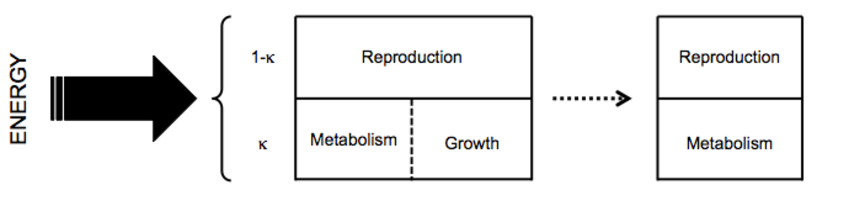
\includegraphics[width=0.95\textwidth]{1_CorpsDeThese/Resumes/Fig/AN01}
\caption[\lofimage{1_CorpsDeThese/Resumes/Fig/AN01}Règle du
$\kappa$]{Schéma de la règle du $\kappa$ et de ses implication}
\label{fig:AN1}
\end{center}
\end{figure}

Outre les interactions entre individus, le modèle se base sur les règles
d'allocation dynamique du budget énergétique \autocites{kooijman2000a}. Une fois la règle fixée, on peut en
dériver les taux vitaux individuels. 

Nous nous basons sur la règle d'allocation appelée règle du
$\kappa$ ($\kappa$-rule), schématisée par la Figure \ref{fig:AN1}. Cette règle
suppose qu'une proportion $\kappa$ de l'énergie acquise par un individu est
allouée à la maintenance (métabolisme) et à la croissance, le reste ($1-\kappa$)
étant attribué à la reproduction. Cela implique automatiquement qu'un individu à sa
taille maximum continue de se reproduire, ce qui n'est pas toujours le cas pour
d'autres règles d'allocation de l'énergie (voir Annexe \ref{An:AmNat},
Supplementary Materials \ref{subsec:SupMat4}). Lorsque l'individu ne grandit
plus, l'énergie est alors divisé en une fraction fixe pour couvrir le
métabolisme et le reste pour la reproduction. Si l'énergie acquise diminue, le
métabolisme étant fixé par la taille de l'individu, la quantité
allouée à la reproduction diminue. Si l'énergie acquise n'est pas suffisante
pour couvrir l'intégralité du métabolisme, l'individu meure.

On suppose que l'acquisition de la ressource est proportionnelle à $l^2$
et que le métabolisme est proportionnel à $l^3$, cette règle d'allocation de
l'énergie nous permet alors de définir les taux vitaux individuels tels que
décrit dans la Table \ref{tab:ANEq}. Le détail de la dérivation des équations du modèle
est disponible dans les Supplementary Materials \ref{subsubsec:SupMat21} de
l'Annexe \ref{An:AmNat}. 

\begin{table}
\centering
\caption{\label{tab:ANEq} Equations du modèle d'après la règle du $\kappa$.}
\begin{tabular}{cl}
\hline 
\hline
&\\
Equation & Description \\
\hline
	$\displaystyle{A(t,l)=1-\frac{\eta(t,l)}{\eta_{H}+\eta(t,l)}}$ & Access to the
	resource\\
	&\\
	$\displaystyle{\eta (t,l) = \int\limits_{l_b}^{l_m} C(l,\lambda)\cdot
	n(t,\lambda)\cdot \lambda^2\,\text{d}\lambda}$ & Experienced population
	density\\
	&\\
	$\displaystyle{C(l,\lambda) = \text{max}[0.01,\, 1+I\cdot(\lambda-l)]}$ &
	Competition function \\
	&\\
	$\displaystyle{g(t,l) = \gamma\cdot(l_m \cdot A(t,l)-l)}$ & Growth rate\\
	&\\
	$\displaystyle{b(t,l) = r_m \cdot A(t,l)\cdot l^2}$ & Birth rate if $l\geq
	l_j$\\
	&\\
	&\\
	$\displaystyle{\frac{\partial n(t,l)}{\partial t}+ \frac{\partial
	g(t,l)\cdot n(t,l)}{\partial l} = -\mu \cdot n(t,l) }$ & Population level
	equation\\
	&\\
	$\displaystyle{g(t,l_b)\cdot n(t,l_b) = \int\limits_{l_b}^{l_m} b(t,l)\cdot
	n(t,l) \, \text{d}l}$ & Boundary conditions \\
\hline 
\end{tabular} 
\end{table}

\subsubsection{Minimum vital d'accès aux ressources}
Nous définissons le minimum vital d'accès aux ressources comme la quantité $A^*$
telle que la croissance individuelle est nulle.

\begin{equation}
\label{eq_an4}
A^*(l) = \frac{l}{l_m}
\end{equation}
Bien que dépendante de $l$,
cette quantité est analogue au $R^*$ de Tilman dans le sens où elle définit des
conditions minimums permettant la croissance des individus. 

Les paramètres utilisés dans ce modèle sont rappelés dans la Table
\ref{tab:ANparam}. Les données expérimentales permettant de justifier ces
données sont présentées dans les Supplementary Materials \ref{subsec:SupMat1} de
l'Annexe \ref{An:AmNat}. 

\begin{table}
\caption{\label{tab:ANparam}Variables et paramètres pour \textit{Folsomia
candida}}
\begin{tabular}{cccl}
\hline
\hline 
 & & &\\
 Objects and  & Default values & Units & Description\\ 
symbols & & &\\
\hline
	$i$-state variable & & & \\ 
	$l$ &   & mm & Individual length \\ 
	Parameters & & & \\ 
	$l_{b}$ & 0.25 & mm & Length at birth \\ 
	$l_{j}$ & 0.6 & mm & Length at maturity \\ 
	$l_{m}$ & 3.0 & mm & Length at infinite\\
	& & &  resources \\ 
	$\gamma$ & 0.015 & d$^{-1}$ & Van Bertalanffy growth rate \\ 
	$\eta_{H}$ & 1000 & individuals & Half saturation constant \\ 
	$\mu$ & 0.0065 & d$^{-1}$ & Background mortality \\ 
	$r_{m}$ & 3.0 & d$^{-1}$mm$^{-2}$ & Reproduction rate \\ 
	$\kappa$ & 0.7 & -- & Fraction of energy \\
	  &   &   & intake allocated \\
	  &   &   & to reproduction \\ 
	  $I$ & 0 & -- & Level of interference\\
\hline 
\end{tabular} 
\end{table}

\subsubsection{Intégration au niveau population}

Au niveau de la population, le nombre d'individus au temps $t$ est donné par
\begin{equation}
\label{eq_an5}
\int_{l_b}^{l_m}\!n(t,l)\,\mathrm{d}l
\end{equation}
où $n(t,l)$ est le nombre d'individus de taille $l$ au temps $t$. La dynamique
de la population est alors donnée par les équations et conditions initiales
suivantes \autocites{kooijman1984a,de-roos1997a}:
\begin{align}
\label{eq_an6}
\frac{\partial n(t,l)}{\partial t}+\frac{\partial g(t,l) \cdot n(t,l)}{\partial l}=-\mu \cdot n(t,l) \\
g(t,l_b) \cdot n(t,l_b)= \int_{l_b} ^{l_m} \! b(t,l)\cdot n(t,l)\, \mathrm(d)l
\\ n(0,l)=\Psi(l)
\end{align}

\subsection{Analyse de bifurcation}

Afin d'étudier le rôle de l'interférence dans les dynamiques produites par notre
modèle, nous avons réalisé une analyse de bifurcation sur le paramètre $I$ du
modèle. Bien que cette analyse ne soit pas une analyse de continuation à
proprement parler, elle nous permet d'identifier les intervalles de paramètre
correspondant à différents types de dynamiques. 

Le principe de cette analyse est comme suit: (i) une première simulation est
exécutée avec la valeur initiale du paramètre dit de bifurcation (ici $I$)
jusqu'à ce que la population ait quitté le régime transitoire; (ii) l'état final
de la population (soit sa distribution à la fin de la simulation) est utilisé
comme état initial d'une nouvelle simulation; (iii) le paramètre d'interférence
est incrémenté; et (iv) le processus est répété jusqu'à exploration de
l'ensemble de l'intervalle voulu. Notons que cette analyse peut également être
réalisée avec des valeurs décroissantes du paramètre de bifurcation, ce qui peut
permettre d'identifier des zones de bistabilité. 

Dans un premier temps, cette analyse a été réalisée pour une valeur fixe des
paramètres excepté le paramètre de bifurcation $I$. Puis, sachant que la
mortalité a un fort effet sur la dynamique de ce type de modèle, cette analyse
a été faite pour des valeurs successives de mortalité avec le paramètre $I$
comme paramètre de bifurcation, et pour des valeurs successives d'interférence
avec le paramètre de mortalité $\mu$ comme paramètre de bifurcation. Ainsi,
l'ensemble de l'espace $(I,\mu)$ a été quadrillé pour des valeurs de $I$ de 0 à
3 et des valeurs de $\mu$ de 0.001 à 0.02

\section{Résultats}

Nous nous intéressons dans un premier temps à l'effet du niveau de compétition
par interférence pour une valeur assez faible de mortalité ($\mu = 0.0065$,
Figure \ref{fig:AN2}). 

\begin{figure}[!ht]
\begin{center}
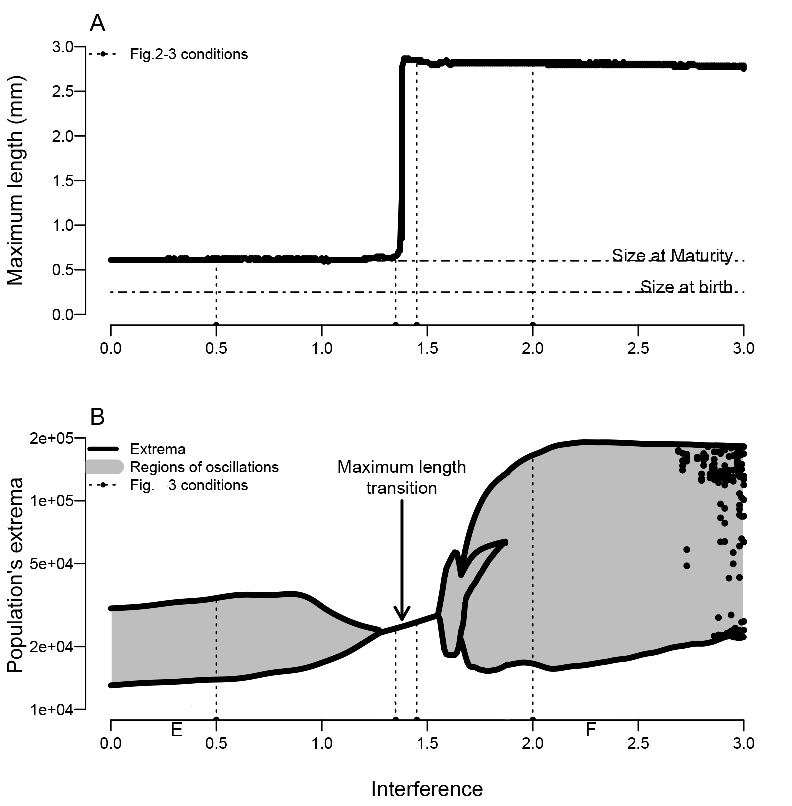
\includegraphics[width=0.95\textwidth]{1_CorpsDeThese/Resumes/Fig/AN02}
\caption[\lofimage{1_CorpsDeThese/Resumes/Fig/AN02}Bifurcation sur le
niveau d'interférence]{Taille maximum atteinte dans la population (A) et extrema
de la population (B, nombre d'individus) en fonction du niveau de compétition par interférence $I$ pour une
valeur constante de mortalité ($\mu = 0.0065$). Les lignes pointillées
représentent les valeur d'interférence des simulations présentées en Figure
\ref{fig:AN3}. Les zones grisées marquent les zones ou la population est
cyclique. La flèche marque la transition de taille maximum atteinte.}
\label{fig:AN2}
\end{center}
\end{figure}

On constate dans un premier temps qu'un niveau suffisamment élevé de compétition
par interférence ($I=1.4$) provoque une transition dans la taille maximum
atteinte par les individus (Figure \ref{fig:AN2}A). Lorsque le niveau
d'interférence est plus faible que cette valeur, la taille maximum atteint ($l=0.63mm$) reste proche de la taille à
maturité ($l_j=0.6mm$). Au delà de la valeur critique, la taille atteinte
($l=2.85mm$) se rapproche fortement de la taille maximum atteignable
($l_m=3mm$). 

De plus, la Figure \ref{fig:AN2}B montre trois régions distinctes: (i) à faible
interférence, la population est cyclique; (ii) pour un niveau intermédiaire de
compétition par interférence, la population est stable; et (iii) pour une forte
interférence, la population cycle autour d'un nouveau type de cycles de plus
grande amplitude que les précédents. 

\subsection{Des cycles dirigés par les juvéniles}

Les modèles PSP classiques prédisent qu'à faible mortalité, la différence de
capacité de compétition entre les juvéniles et les adultes conduit à des cycles
de génération dirigés par les juvéniles \autocites{de-roos1992a,de-roos1997a}.
La Figure \ref{fig:AN3}abc montre la dynamique de la population pour un faible
niveau d'interférence ($I=0.5$). On observe sur le diagramme structure-temps (a)
que la dynamique cyclique correspond à des vagues successives de recrutement de
juvéniles avec des adultes ne dépassant que très peu la taille à maturité. Cette
dynamique est caractéristique des cycles de génération dirigés par les juvéniles
\autocites{de-roos1992a,de-roos2003a}.

\afterpage{%
    \clearpage% flush all other floats
    \ifodd\value{page}
    %\else% uncomment this else to get odd/even instead of even/odd
        \expandafter\afterpage% put it on the next page if this one is odd
    \fi
    {%
    \begin{figure}[p]
        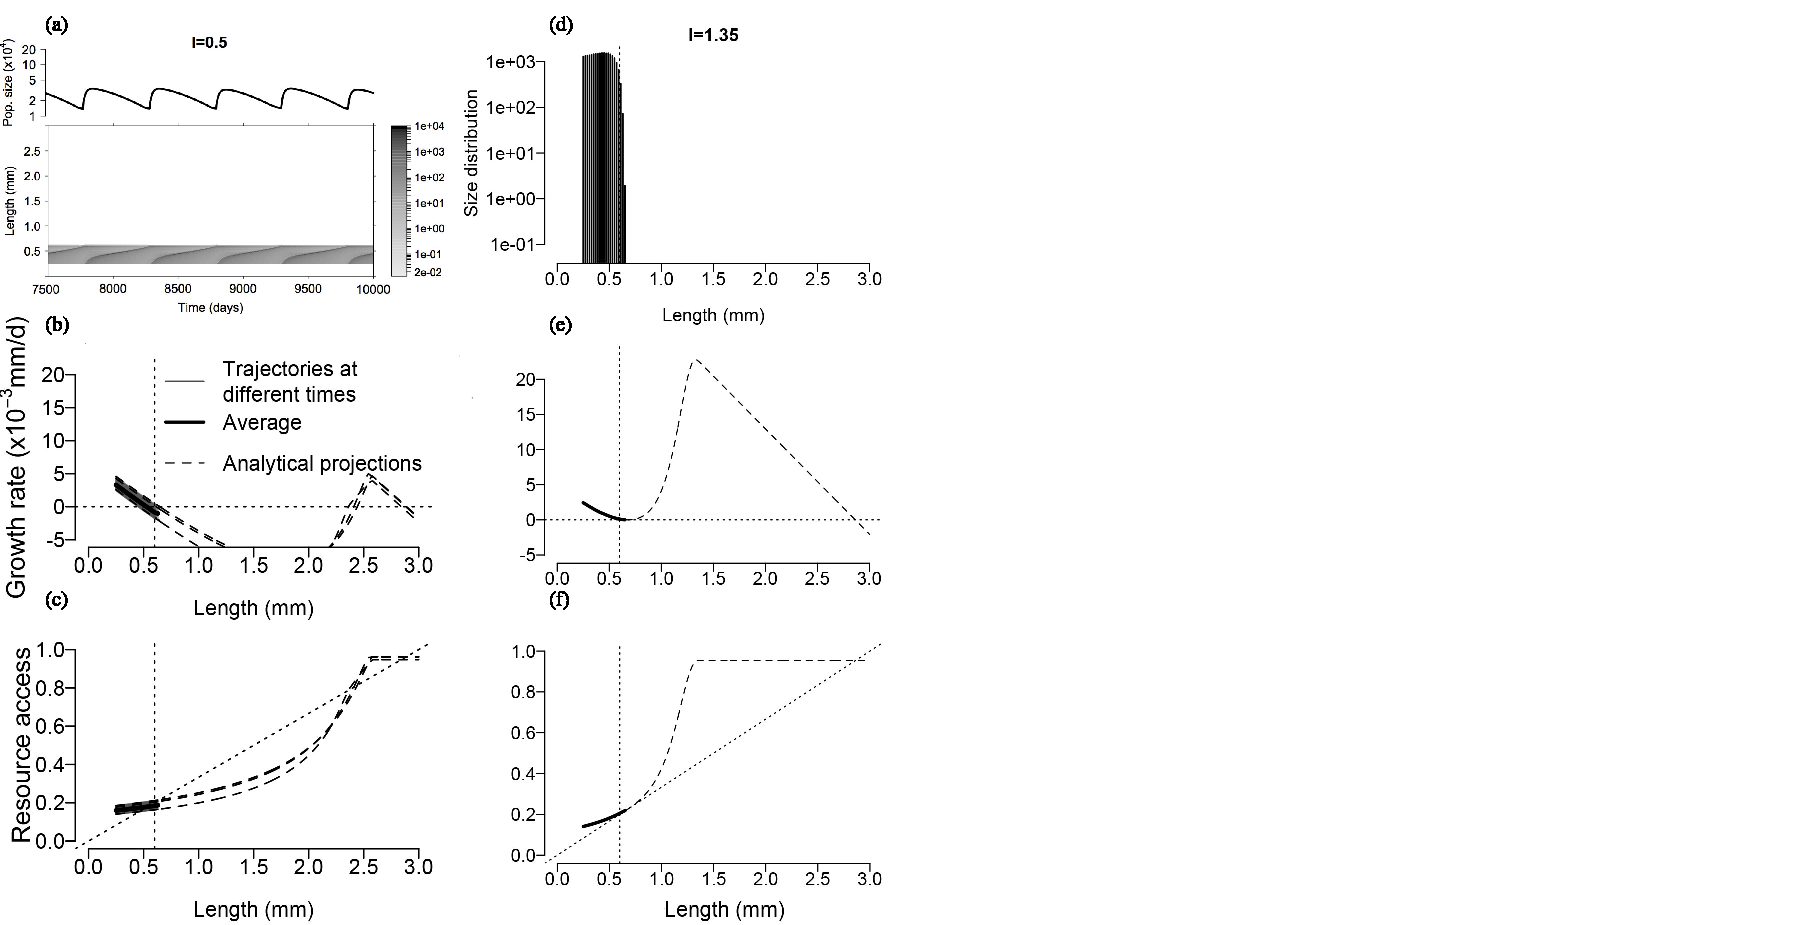
\includegraphics[width=\textwidth]{1_CorpsDeThese/Resumes/Fig/AN03}
        \caption[\lofimage{1_CorpsDeThese/Resumes/Fig/AN03}Exemples de
        dynamiques pour quatre valeurs d'interférence]{Exemples de dynamiques pour quatre valeurs d'interférence:
        0.5, 1.5, 1.45 et 2.0. La première ligne de panels (a,d,g,j) montre soit la
dynamique de la structure à l'aide d'un diagramme structure-temps (a,j), soit la
distribution de la taille si elle est stable dans le temps (d,g). La seconde
ligne (b,e,h,k) représente le taux de croissance en fonction de la longueur
corporelle\ldots}\label{fig:AN3}
    \end{figure}
    \clearpage
    \begin{figure}[p]
		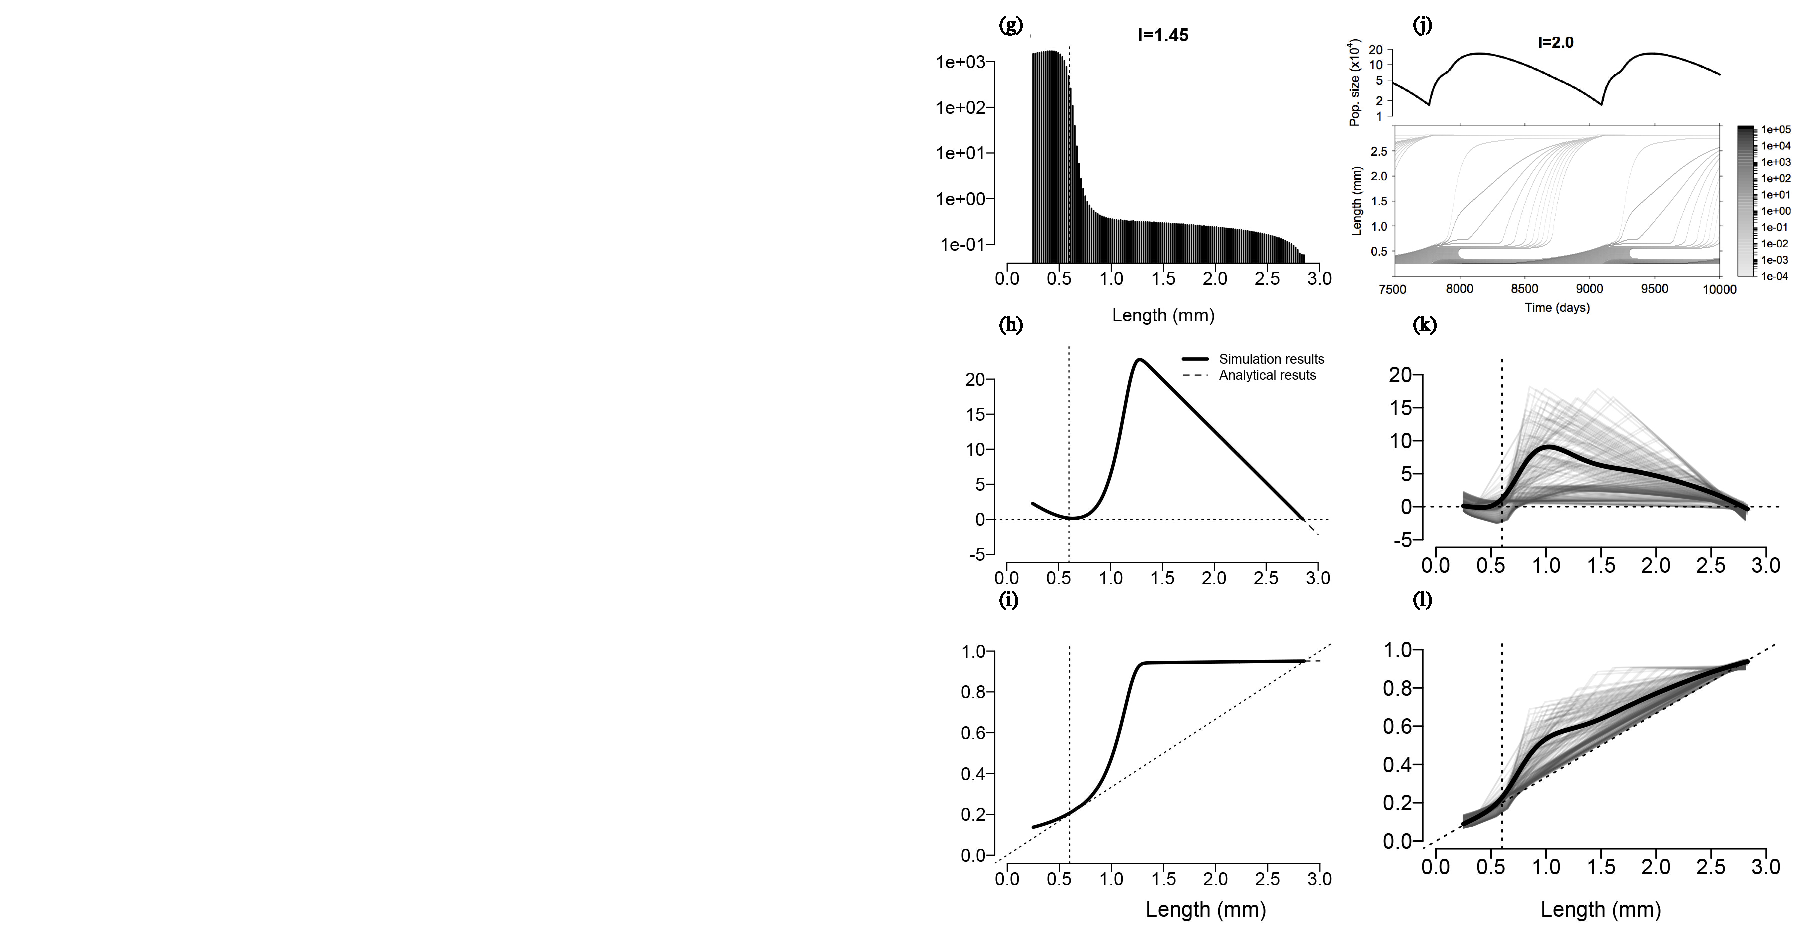
\includegraphics[width=\textwidth]{1_CorpsDeThese/Resumes/Fig/AN04}
        \caption*{\ldots Lorsque la dynamique est cyclique, plusieurs
        trajectoires sont présentées, ainsi que leur moyenne en trait épais.La ligne pointillée
horizontale est le 0, la ligne verticale marque la taille à maturité. Enfin, la
dernière ligne de panels (c,f,i,l) présente l'accès à la ressource. La ligne
verticale marque la taille à maturité, la ligne oblique marque l'accès minimum
requis $A^*$. Pour le taux de croissance et l'accès aux ressources, les lignes
tiretées représentent les projections analytique des fonctions tracées.}
    \end{figure}
    \clearpage
    }%
}

Les Figures \ref{fig:AN3}b et c montrent le taux de croissance et l'accès aux
ressources pour cette dynamique. Le taux de croissance décroît
quasi-linéairement avec la taille, de façon très similaire au modèle classique
sans interférence. L'accès aux ressources est très légèrement croissant mais
devient rapidement inférieur à $A^*$ pour tous les individus après la maturité. 

\subsection{Un équilibre stable avec des petits ou des géants}

Pour des valeurs intermédiaires de compétition par interférence, l'avantage
que les grands individus retirent de l'interférence contrebalance la compétition
par exploitation imposée par les juvéniles. Ceci vient contrer les mécanismes
de déséquilibre compétitif à l'origine des cycles de génération, et tend à
stabiliser la population (Figure \ref{fig:AN3}d-i).

Pour une valeur d'interférence sous le seuil critique de $I=1.4$, la dynamique
se stabilise autour d'une distribution étroite de la taille corporelle (Figure
\ref{fig:AN3}d). Le taux de croissance et l'accès à la ressource ont tendance à
se courber vers le haut pour les plus grands individus, mais la courbure n'est
pas suffisante pour permettre à l'accès au ressources de rester au dessus de
$A^*$, et les individus s'arrêtent de grandir rapidement après la maturation (Figure
\ref{fig:AN3}ef).

Au delà de ce seuil critique, la courbure est suffisante pour que l'accès aux
ressources soit toujours supérieur à $A^*$ et le taux de croissance soit
toujours positif (Figure \ref{fig:AN3}hi). Après un ralentissement de leur
croissance proche de la maturité (``goulet d'étranglement de la croissance''), les individus peuvent
reprendre une croissance rapide jusqu'à des tailles très élevées. La
distribution de la taille dans la population est alors très asymétrique vers les
juvéniles, mais reste continue jusqu'à des tailles proches de la taille maximum
possible $l_m$ (Figure \ref{fig:AN3}g). Les formes particulières des fonctions
de croissance et d'accès à la ressource s'expliquent d'abord par la faible
densité d'adultes au delà de $0.6mm$ et leur grande compétitivité, ils
sont donc rapidement capables de monopoliser la ressource et grandissent très
rapidement. La partie linéaire après $l=1.4mm$ est quand a elle la conséquence
de la forme naturelle de la fonction de croissance de Von Bertalanffy. 

\subsection{Des cycles induits par l'interférence}

La bifurcation sur l'interférence montre l'apparition de cycles lorsque le
niveau de compétition par interférence est suffisamment élevé ($I>1.56$ Figure
\ref{fig:AN2}). La Figure \ref{fig:AN3} (j-l) montre le détail de la dynamique
pour une valeur de compétition par interférence de $I=2.0$. On constate sur le
diagramme structure temps (j) que les cycles dans la structure de la population
sont très différents des cycles de génération induits par les juvéniles (a). La
période des cycles a été multipliée par $3$ et l'amplitude est environ $7.5$
fois supérieure. Un cycle dans la dynamique commence par un pulse de naissance
qui fait fortement augmenter la taille de la population lorsqu'une cohorte
d'individus atteint la maturité. La population est alors multi-modale avec une majorité
de juvéniles, des adultes nouvellement matures et quelques vieux individus de
très grande taille. Après le pulse de naissance, les individus qui viennent de
maturer grandissent, ce qui réduit la ressource disponible pour les individus
les plus petits qui stoppent leur croissance. Deux groupes se forment, des
juvéniles de moins de $0.35mm$ et des juvéniles et jeunes adultes entre $0.5$ et
$0.75mm$. Pendant cette période, les adultes continent de se reproduire,
augmentant la densité de juvéniles. Les individus les plus vieux commencent
ensuite à mourir, diminuant progressivement la pression de compétition sur les
jeunes adultes qui atteignent à leur tour des tailles extrêmes. La pression de
compétition est cependant maintenue sur les plus petits juvéniles qui ne peuvent
pas grandir. Le nombre d'individus reproducteur commence alors à diminuer,
réduisant progressivement la taille de la population et la pression de
compétition due à l'interférence. Quand suffisamment d'adultes sont mort, la
pression de compétition a assez diminué pour que les plus petits juvéniles
reprennent leur croissance et maturent, provoquant un nouveau cycle dans la
dynamique. 

On constate sur le panel (k) que la position du goulet d'étranglement du taux de
croissance sur l'axe des X varie entre $0.33$ et $0.55mm$ suivant le moment dans
le cycle, mais reste systématiquement inférieur à la taille à maturité
$l_j=0.6mm$, ce qui provoque l'accumulation d'individus immature dans la
population. L'accès aux ressources (l) montre le même phénomène. Les individus
n'accèdent plus suffisamment aux ressources pour poursuivre leur croissance dont
le taux devient négatif (causant une mortalité accrue). Ils arrêtent donc leur
croissance à un stade immature, ce qui fait diminuer le nombre de reproducteur
et relâche progressivement la pression de compétition par interférence. C'est
précisément la position du goulet d'étranglement sous la taille à maturité qui
déstabilise la dynamique vers ces nouveaux cycles. 

\subsection{Bifurcation dans le plan $(I,\mu)$}

Le taux de mortalité basal $\mu$ étant connu pour affecter la dynamique des
populations structurées par taille, en stabilisant la dynamique vers un point
fixe lorsqu'il augmente, nous nous somme intéressé à son effet couplé à celui du
niveau de compétition par interférence. La Figure \ref{fig:AN4} montre le type
de dynamique obtenu en fonction de la position dans le plan de paramètres
$(I,\mu)$.

\begin{figure}[!ht]
\begin{center}
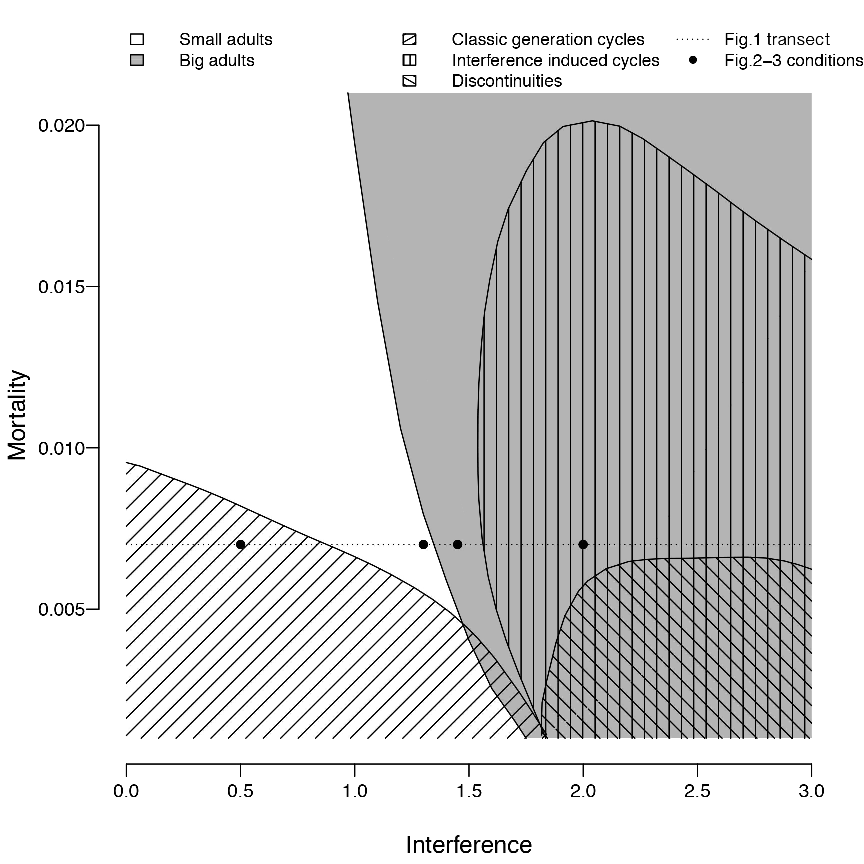
\includegraphics[width=0.95\textwidth]{1_CorpsDeThese/Resumes/Fig/AN05}
\caption[\lofimage{1_CorpsDeThese/Resumes/Fig/AN05}Diagramme de
bifurcation dans le plan $(I,\mu)$]{Diagramme de
bifurcation dans le plan $(I,\mu)$. Les régions sans hachure sont les régions
correspondant à un point fixe. Les hachures représentent le type de cycle
obtenu. La zone grise correspond à la zone de survie des individus de très
grande taille. La ligne pointillée et les points marquent respectivement la
bifurcation de la Figure \ref{fig:AN2} et les simulations de la Figure
\ref{fig:AN3}}
\label{fig:AN4}
\end{center}
\end{figure}

Dans un premier temps, on peut distinguer deux régions différentes sur ce
diagramme (régions blanches et grises) qui délimitent les zones où
la taille maximale atteinte est soit proche de la taille à maturité (en blanc),
soit proche de la taille maximum possible (en gris). Il est intéressant de noter
que la limite entre ces deux régions dépend assez peu de la mortalité basale
( $I$ entre $1.2$ et $1.6$).

On remarque également qu'en l'absence d'interférence, les cycles de génération
induits par les juvéniles sont stabilisés lorsque la mortalité basale augmente,
conformément à la théorie déjà établie \autocites{de-roos1997a}. Lorsque la
compétition par interférence est présente, cette stabilisation se produit pour
des valeurs plus basses de mortalité. De plus, l'augmentation du taux de
mortalité semble également stabiliser les cycles due à l'interférence, mais pour
des valeur très élevées ($\mu > 0.02$). 

A faible mortalité mais haut niveau d'interférence, la dynamique est irrégulière
et les résultats sont peu fiables à cause de problèmes numériques liés à
l'intégration des équations du modèle. En revanche, pour une interférence
intermédiaire et une faible mortalité, on peut observer une situation
intéressante. En effet, on constate qu'il existe une petite région où des cycles
de génération semblables à ceux dues aux juvéniles se maintiennent alors que la
taille maximum atteinte est proche de la taille maximum possible. Mais ces
cycles sont dégénérés et quelques individus parviennent de temps en temps à
s'échapper du goulet de croissance et atteindre des tailles géantes. Ces
individus sont rares et les dynamiques irrégulières. 

\section{Discussion}

Nous avons mis en évidence au cours de cette étude que la compétition par
interférence est une interaction qui, en conférant un avantage aux individus les
plus grands, vient contrecarrer les effets de la compétition taille dépendante
par exploitation. La dépendance à la taille de l'ingestion d'énergie et de son
utilisation confère un avantage aux individus les plus petits par la compétition
par exploitation \autocites{peters1986a,persson1998a,de-roos2013a} comme le
prédit la théorie du budget énergétique dynamique \autocites{kooijman2000a}.
Dans l'intervalle de niveaux de compétition par interférence que nous étudions
ici, l'équilibre compétitif entre les plus petits et les plus grands individus
bascule progressivement d'un avantage aux juvéniles, du à la compétition par
exploitation, à un avantage aux grands adultes, du à la compétition par
interférence. Entre les deux extrêmes, les compétitions par exploitation et
interférence s'équilibre et la population se stabilise. Les transitions observée
dans la Figure \ref{fig:AN2} sont très comparables à celles causées par des
modifications de la dépendance en taille de la compétition par exploitation,
telles que l'augmentation des pentes des fonctions allométriques pour le taux
d'attaque \autocites{persson1998a} ou pour le taux de consommation
\autocites{de-roos2003a}. Cependant, les mécanismes sous jacents restent très
différents. En effet, la transition vers des cycles dominés par les adultes dans
les études de \textcites{persson1998a} et \textcites{de-roos2003a} se produisent
pour des valeurs de paramètre peu réalistes. Déjà prédite par
\textcites{de-roos2003a}, notre étude propose une hypothèse alternative
conduisant à des cycles de génération dominés par les adultes.

Bien que les cycles induits par l'interférence ne soient pas strictement des
cycles dominés par les adultes (``adult driven generation cycles'') selon la
définition de \textcites{de-roos2003a}, ils partagent avec eux une
caractéristique essentielle, à savoir le fait que les oscillation reposent sur
la domination compétitive des individus les plus grands qui empêchent une
nouvelle génération de dominer la population tant qu'ils sont suffisamment
nombreux. Dans ce sens, les cycles induits par l'interférence font partie
des cycles dominés par les adultes.  

\subsection{Détecter la compétition par interférence dans des populations
naturelles} 

Le cannibalisme est un autre mécanisme qui confère un avantage aux
plus grands individus d'une population sur les plus petits en les protégeant de la
compétition par exploitation \autocites{claessen2000a,claessen2002a}, et peut
ainsi conduire à la stabilisation des cycles dominés par les juvéniles et
l'émergence d'individus de grande taille. Ces similarités font qu'il est
nécessaire d'avoir des clés permettant de discriminer différentes causes pouvant
mener aux même observations dans des populations naturelles. 

D'après nos résultats théoriques, plusieurs critères peuvent être utilisés pour
identifier le rôle de la compétition par interférence dans la dynamique d'une
population structurée. 
\begin{enumerate*}[label=(\roman*)]
\item L'observation la plus évident de l'effet de l'interférence est l'émergence
de géants dans la population. Bien que d'autres cause puissent provoquer cette
émergence telles que le cannibalisme ou une niche spécifique pour les plus
grands individus, combiné aux éléments suivant, c'est un indice en faveur
de la compétition par interférence. 
\item La présence d'un goulet d'étranglement de la croissance est un signe fort
de l'action d'une compétition par interférence assez intense.
\item Ce goulet d'étranglement provoque une distribution de la taille
fortement asymétrique en faveur des plus petits individus dans une population
stable. 
\item Dans une population cyclique, cela résulte en une distribution
multi-modale.
\item Dans les deux cas, les trajectoires de croissance individuelles
ressemblent à une double courbe de croissance. Les individus subissent un
ralentissement violent de la croissance autour de la maturité avant une
accélération brutale passé le goulet d'étranglement. 
\item L'observation des traits d'histoire de vie individuels permets donc de
distinguer les cycles causés par l'interférence des cycles dominés par les
juvéniles. Dans le dernier cas, les individus grandissent rapidement et
s'arrêtent après maturation alors que dans le premier cas la croissance s'arrête
vers la maturation pour ne reprendre que si la cohorte adulte dominante a
suffisamment diminuée. 
\item Enfin, dans le cas où les données individuelles ne sont pas accessibles,
le ratio du temps de maturation moyen par la période des cycles tel que défini
par \textcites{murdoch2002a} permet également de faire la distinction entre les
différents cycles. Comme expliqué en introduction de cette thèse
(Section \ref{modelPopStru} page \pageref{modelPopStru}), une valeur du ratio
autour de $1$ correspond à des cycles de génération. Dans notre modèle, les
cycles dominés par les juvéniles ont un ratio autour de $0.8$ alors que les cycles induits par l'interférence ont un
ratio proche de $1.5$. Ainsi, des cycles de génération avec un ratio supérieur
à 1 pourraient être une indication du rôle de l'interférence. Cela pourrait par
exemple être le cas pour les saumons dans la baie de Bristol (ratio$=1.2$) ou de
la rivière Togiak ($1.3$), la morue d'Iceland ($1.6$), le castor de Californie
(1.6), ou l'ours noir du Yukon \autocites[1.5,][]{murdoch2002a}. Ces espèces
étant territoriales, elles sont en effet susceptibles à la compétition intra-spécifique par interférence. 
\end{enumerate*}

\subsection{L'interférence dans nos populations expérimentales}

Nous avons montré dans le Chapitre \ref{chap:sp} que nos populations
expérimentales de collemboles se caractérisent systématiquement par
l'existence de plusieurs modes dans la distribution de la taille des individus.
Généralement deux, un mode assez dense de juvéniles dont la taille est proche de
la taille à la naissance, et un mode d'adultes dont la taille est très
supérieure à la taille à maturité (parfois jusqu'à plus de trois fois
supérieur). Exceptionnellement, un troisième mode peut être observé, on a alors
un premier mode de juvéniles, un mode avec des petits adultes et un mode avec
des grands adultes. Mais nous avons montré que cette situation n'était stable
que localement, et ne pouvait être atteinte qu'avec des conditions initiale de
distribution de la taille très particulières qui ne se retrouvent quasiment
jamais hors de l'initialisation des populations.

De plus, nous avons montré que les individus de grande taille jouent un rôle
prépondérant dans la dynamique de la population notamment en empêchant la
croissance des juvéniles lorsque les cohortes d'adultes sont suffisamment
denses. 

Ces observations recoupent ainsi plusieurs des critères proposés à l'issue de
notre étude théorique pour identifier le rôle de la compétition par
interférence. Cette analyse apporte des arguments supplémentaires pour confirmer
le rôle de la compétition par interférence dans la dynamique des populations de
collemboles, et confirment ainsi du même fait l'intérêt des méthodes empiriques
employées dans l'étude précédente pour extraire le rôle de
l'interférence des données.

\section{En conclusion}

Notre objectif était ici d'étudier les conséquences de la compétition taille
dépendante par interférence sur la dynamique des populations, permettant ainsi
de compléter les résultats existants sur la compétition par exploitation et le
cannibalisme comme mécanismes intra-spécifiques de régulation des populations.
Nous avons donc développé un modèle simple de dynamique de populations physiologiquement
structurées qui à notre avis rassemble les aspects essentiels de la compétition
intra-spécifique par interférence. Ce modèle n'a ainsi pas pour vocation de
prédire précisément des dynamiques de populations, bien qu'il ait été paramétré
pour les Collemboles \textit{Folsomia candida}, mais plutôt de démontrer les
conséquences dynamiques de la compétition par interférence. La comparaison avec
nos données expérimentales issues des populations de collemboles montre qu'il
est possible de détecter le rôle de la compétition par interférence dans des
populations expérimentales ou naturelles. 

Dans notre cas, nous avons pu apporter de nouveaux éléments confirmant le rôle
de la compétition par interférence dans les dynamiques des populations de
collemboles, mais il reste encore des différences entre le modèle et les séries
temporelles observées, et les mécanismes détaillés à l'oeuvre dans les
populations expérimentales ne sont encore pas éclaircis. Dans le Chapitre
suivant, nous avons mené en parallèle deux études expérimentales afin de mieux
comprendre la façon dont les individus se répartissent l'accès à la ressource,
et le rôle des individus de différentes tailles dans la dynamique de la structure
des populations.


\chapter{Confirmation du rôle de l'interférence: modification de la structure
des populations et observation de l'accès aux ressources}
\chaptermark{Confirmation du rôle de l'interférence}
\label{chap:sm}

\vspace{5cm}

\section{Introduction}

\lettrine[lines=3]{N}{otre} étude de l'effet des interactions entre individus
dans la dynamique des populations structurées nous a mené dans le Chapitre
\ref{chap:sp} à proposer la
compétition par interférence comme mécanisme responsable de la structuration
multimodale de nos populations expérimentales de collemboles \textit{Folsomia
candida} (voir aussi Annexe \ref{Ann:SP}). Au cours du Chapitre
\ref{chap:amnat} (voir aussi Annexe \ref{An:AmNat}), nous avons étudié dans un
modèle théorique les conséquences d'une compétition par interférence plus ou moins intense sur la dynamique d'une population structurée où la compétition par
exploitation entre également en jeu. Nous avons montré qu'une compétition par
interférence suffisamment intense pouvait être à l'origine d'une stabilisation
des cycles de génération dominés par les juvéniles, puis de l'apparition de
cycles de plus longue période au cours des quels des individus parviennent à
atteindre de très grandes tailles, et où la population a une structure
multimodale. Ces deux études semblent donc montrer que la compétition par
interférence est un mécanisme suffisant pour l'apparition de distributions
multimodales dans des populations structurées par la taille, et la survie
d'individus à des tailles bien supérieures à leur taille à maturité.

Suite aux résultats de notre étude théorique, nous avons voulu vérifier dans nos
populations expérimentales quel était le rôle précis des individus de
différentes tailles dans les dynamiques des structures observées, afin de
pouvoir affirmer le rôle de la compétition par interférence avec plus de certitudes.
Pour ce faire, nous avons mené deux expériences en parallèle. Dans une première
expérience nous sommes intervenus sur des populations dont la dynamique semblait
stable en perturbant la structure de la population afin d'en observer le retour
à l'équilibre et de pouvoir comparer la situation finale à celle avant la
perturbation. Cette expérience a été réalisée sur les deux clones étudiés
jusque-là, HA et TO.

Dans une seconde expérience nous nous sommes intéressés aux comportements
d'accès à la ressource dans les populations. Nous avons réalisé une série
d'observations en temps réel dans les populations afin de mieux comprendre
comment la ressource était partagée entre les individus d'une population. Ces
observations ont été réalisées dans certaines des populations de la première
expérience. Elles ont permis de comparer la distribution en taille des individus
accédant à la ressource à celle de l'ensemble de la population au moment de
l'observation. Cette comparaison a mis en évidence un accès différentiel en
fonction de la taille avec un biais quasi-systématique en faveur des individus
les plus grands dans l'accès à la ressource. 

\section{Matériel et méthodes}

\subsection{Perturbation de la structure d'une population}

Dans la première expérience, nous avons suivis des populations de collemboles
\textit{Folsomia candida} jusqu'à stabilisation de leur structure, puis nous
avons perturbé la structure afin d'observer le retour à un régime permanent. 

\subsubsection{Les populations étudiées}

Nous avons élevé et dénombré régulièrement $16$ populations de collemboles, $8$
du clone HA et $8$ du clone TO, pendant un an jusqu'à stabilisation de la
structure. Les populations ont été élevées à $21\degres$C dans les conditions
décrites dans le Chapitre \ref{chap:method}. Les populations ont été mesurées
régulièrement pour suivre leur structure en suivant également la méthode de
phénotypage haut débit présentée précédemment (voir Chapitre \ref{chap:method}
Section \ref{sec:bpsensor} et Annexe \ref{Ann:bpsensor}).

\subsubsection{Perturbation de la structure}

\paragraph{Témoins} Après 12 mois, nous considérons que la période transitoire
de la dynamique est terminée. La perturbation de la structure que nous imposons
aux populations fait intervenir un changement de boite d'élevage. Afin de
vérifier l'impact d'un changement de boite sur la dynamique de la structure
d'une population, nous conservons deux témoins pour chacun des clones pour les
quels la structure n'est pas modifiée mais la population est intégralement
transférée dans une nouvelle boite d'élevage.

\paragraph{Clone HA} Avant la perturbation de la structure les populations du
clone HA ont toutes convergé vers une distribution tri-modale de la taille
corporelle. Nous avons donc réalisé trois traitements différents, chacun sur
deux populations. Chaque traitement consiste à diviser une population en deux en
fonction de la taille des individus. La structure de la population étant séparée
en trois modes, un des modes est prélevé et isolé dans une nouvelle boite
d'élevage, tandis que les deux autres sont conservés ensemble et également
transférés dans une nouvelle boite.

Les trois modes des distributions sont désignés respectivement par les lettres J
(ou Je) pour les juvéniles, M (ou Mo) pour le premier mode d'adultes de
taille moyenne, et G (ou Gd) pour le mode d'adultes de grande taille. Les
différents traitements consistent donc à \begin{enumerate*}[label=(\roman*), before=\unskip{ : }, itemjoin={{ ; }},
itemjoin*={{ ; et }}]
\item isoler la cohorte Je et conserver les cohortes M et G dans une population
MG
\item isoler la cohorte Mo et conserver les cohortes J et G dans une population
JG
\item isoler la cohorte Gd et conserver les cohortes J et M dans une population
JM (Figure \ref{fig:SM0}).
\end{enumerate*} 
Après la séparation des cohortes, les populations nouvellement fondées sont
replacées dans les conditions d'élevage habituelles et dénombrées et mesurées
régulièrement pendant $15$ mois pour observer la période de transition et le
retour à une structure stable. 

\begin{figure}[!ht]
\begin{center}
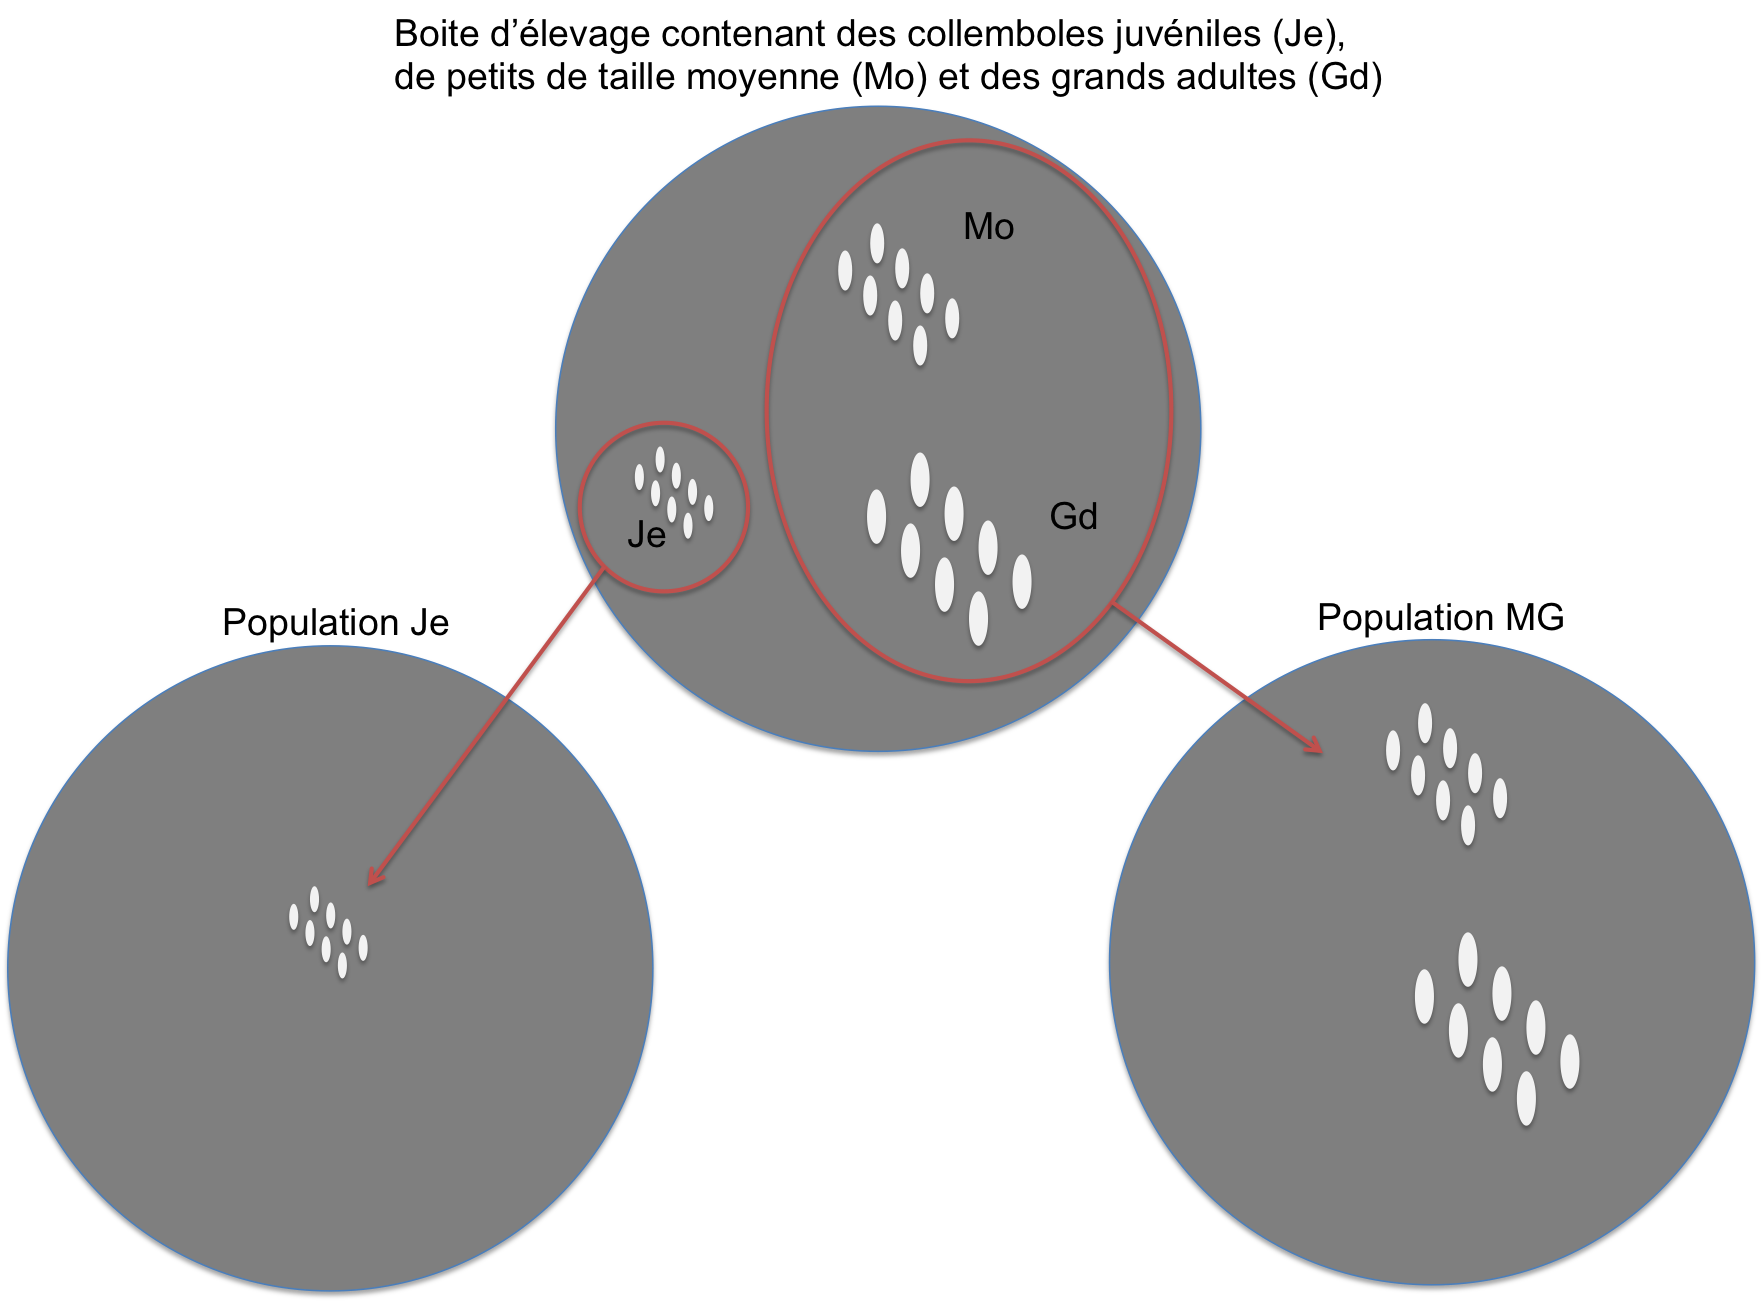
\includegraphics[width=1\textwidth]{1_CorpsDeThese/Resumes/Fig/SM00}
\caption[\lofimage{1_CorpsDeThese/Resumes/Fig/SM01}Exemple de
séparation d'une population]{Exemple de
séparation d'une population pour un traitement Je - MG.}
\label{fig:SM0}
\end{center}
\end{figure}


\paragraph{Clone TO} Contrairement au clone HA, les populations du clone TO ont
convergé au cours de la première phase de l'expérience vers des structures
bimodales. L'analyse des populations HA a montré que les adultes se répartissent
en moyenne en $\frac{2}{3}$ de petits adultes et $\frac{1}{3}$ de grands
adultes. Afin de conserver des manipulations comparables entre les clones HA et
TO, et mettre les nouvelles populations dans des conditions similaires entre les
deux clones, nous avons décidé de séparer la cohorte d'adultes en un groupe
contenant deux tiers des individus (M) et un groupe contenant le tiers restant
(G) afin de suivre les mêmes traitements que pour le clone HA. Les individus
sont choisis au hasard pour être attribué à M ou G.
Ainsi, les traitements sont \begin{enumerate*}[label=(\roman*), before=\unskip{ : }, itemjoin={{ ; }},
itemjoin*={{ ; et }}]
\item isoler la cohorte Je et conserver ensemble tous les adultes (MG)
\item isoler deux tiers des adultes (Mo) et conserver les cohortes J et le reste
des adultes G (JG)
\item isoler un tiers des adultes (Gd) et conserver les cohortes J et deux tiers
des adultes M (JM).
\end{enumerate*} 
Les nouvelles populations sont suivies pendant $15$ mois pour observer la phase
transitoire et observer le nouvel équilibre. 

\begin{figure}[!ht]
\begin{center}
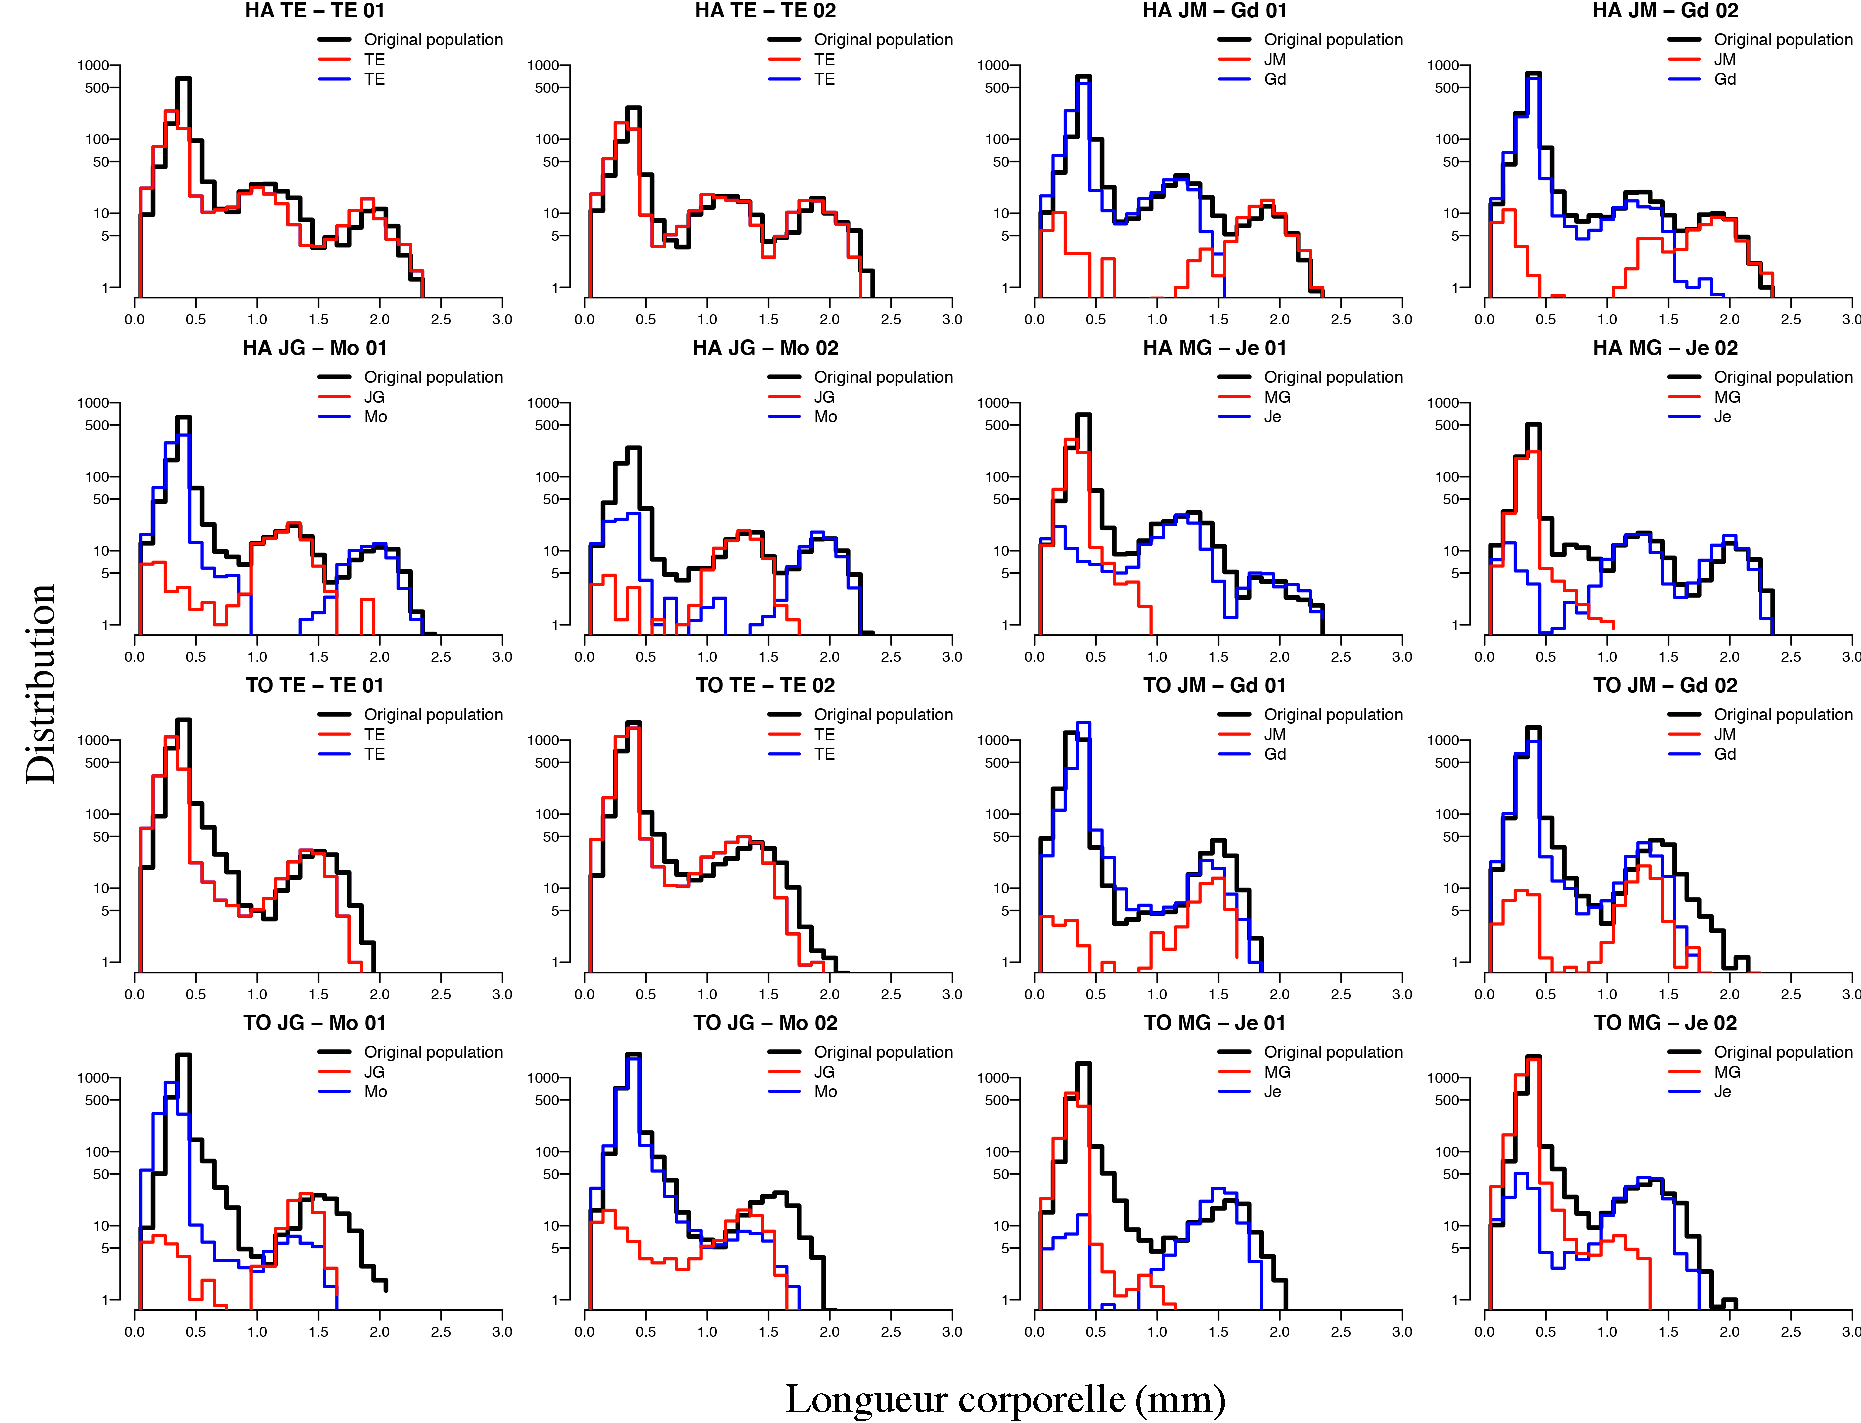
\includegraphics[width=1\textwidth]{1_CorpsDeThese/Resumes/Fig/SM01}
\caption[\lofimage{1_CorpsDeThese/Resumes/Fig/SM01}Séparation des
populations]{Résultat de la séparation des populations en deux en fonction de
la taille des individus. La ligne noire est la population d'origine, les lignes
bleues et rouges sont les populations séparées. Je, Mo et Gd se réfèrent
respectivement aux cohortes J, M et G.}
\label{fig:SM1}
\end{center}
\end{figure}

Afin de vérifier le résultat des séparations des populations en deux, nous avons
tracé pour chaque population, sur un même graphique, la distribution de la
taille dans la population d'origine et dans chacune des deux nouvelles
populations. L'ensemble des graphiques obtenus est présenté sur la Figure
\ref{fig:SM1}

\subsubsection{Analyse des dynamiques}

Les dynamiques des structures avant et après perturbation sont analysées grâce
aux diagrammes structure-temps (Chapitre \ref{chap:method} Section \ref{sec:stdiag} et
Annexe \ref{Chap:STDiag}).
Les structures après stabilisation sont alors comparées aux structures avant perturbation et
aux autres traitements. 

\subsection{Accès à la ressource}

Dans la seconde expérience de cette étude, nous réalisons une série d'analyses
\textit{in-situ} des comportements d'accès aux ressources.

\subsubsection{Observations comportementales}

La ressource est composée d'une pastille de quelques millimètres de diamètre de
levure de bière dissoute dans 15$\mu$L d'agar-agar. Afin d'observer les
comportements individuels d'accès à cette ressource, nous avons placé les boites
observées dans une étuve à 21$\degres$C, sous un microscope USB permettant une
observation en temps réel de la surface de la boite. Nous avons alors pris une
série de 10 photographies de la zone de la boite contenant la pastille de
ressource. Les clichés ont été pris avec 15 minutes d'intervalle afin de pouvoir
considérer une indépendance temporelle entre les photos. Au cours de ces
observations, la pastille est principalement consommée par le dessus, la surface
de ressource accessible pendant la période d'observation varie donc peu.

\begin{figure}[!ht]
\begin{center}
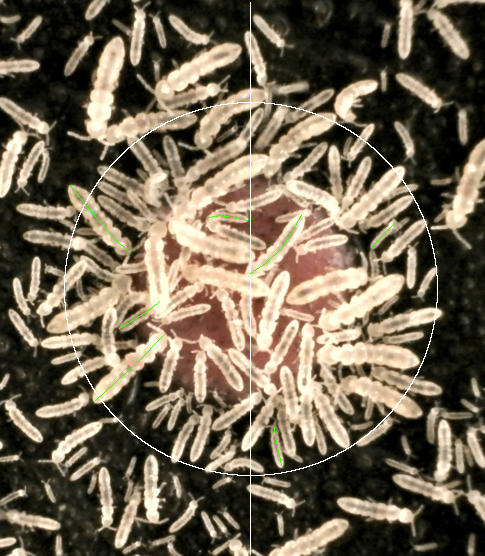
\includegraphics[height=0.25\textheight]{1_CorpsDeThese/Resumes/Fig/SM01b}
\caption[\lofimage{1_CorpsDeThese/Resumes/Fig/SM01}Exemple de comptage
sur une pastille]{Exemple de comptage
sur une pastille, les individus inclus dans le cercle sont comptés,
partiellement ou totalement à gauche, totalement uniquement à droite. Les
lignes vertes montrent le comptage et la mesure de quelques individus.}
\label{fig:SM1b}
\end{center}
\end{figure}

Les séries de photographies récoltées permettent de mesurer la taille des
individus accédant à la ressource à 10 moments que l'on considère indépendants.
L'ensemble des individus accédant à la ressource est mesuré à la main à l'aide
du logiciel d'analyse d'image ImageJ (Figure \ref{fig:SM1b}). Sur chacune des
photos analysées, la pastille est coupée verticalement en deux. Sur une des moitiés, l'ensemble des
individus en contact avec la pastille sont comptés, qu'ils soient partiellement
ou intégralement sur la pastille. Sur la seconde moitié, seuls les individus
intégralement sur la pastille sont mesurés. Ainsi on obtient dix distributions
de la taille des individus accédant à la ressource, dont on compare la moyenne à
la distribution de la taille dans la population totale.

\subsubsection{Mesure du biais d'accès aux ressources}

La distribution de la taille des individus accédant à la ressource comparée à
celle dans la population totale nous permet de mesurer un biais de taille
corporelle dans l'accès aux ressources.

\begin{figure}[!ht]
\begin{center}
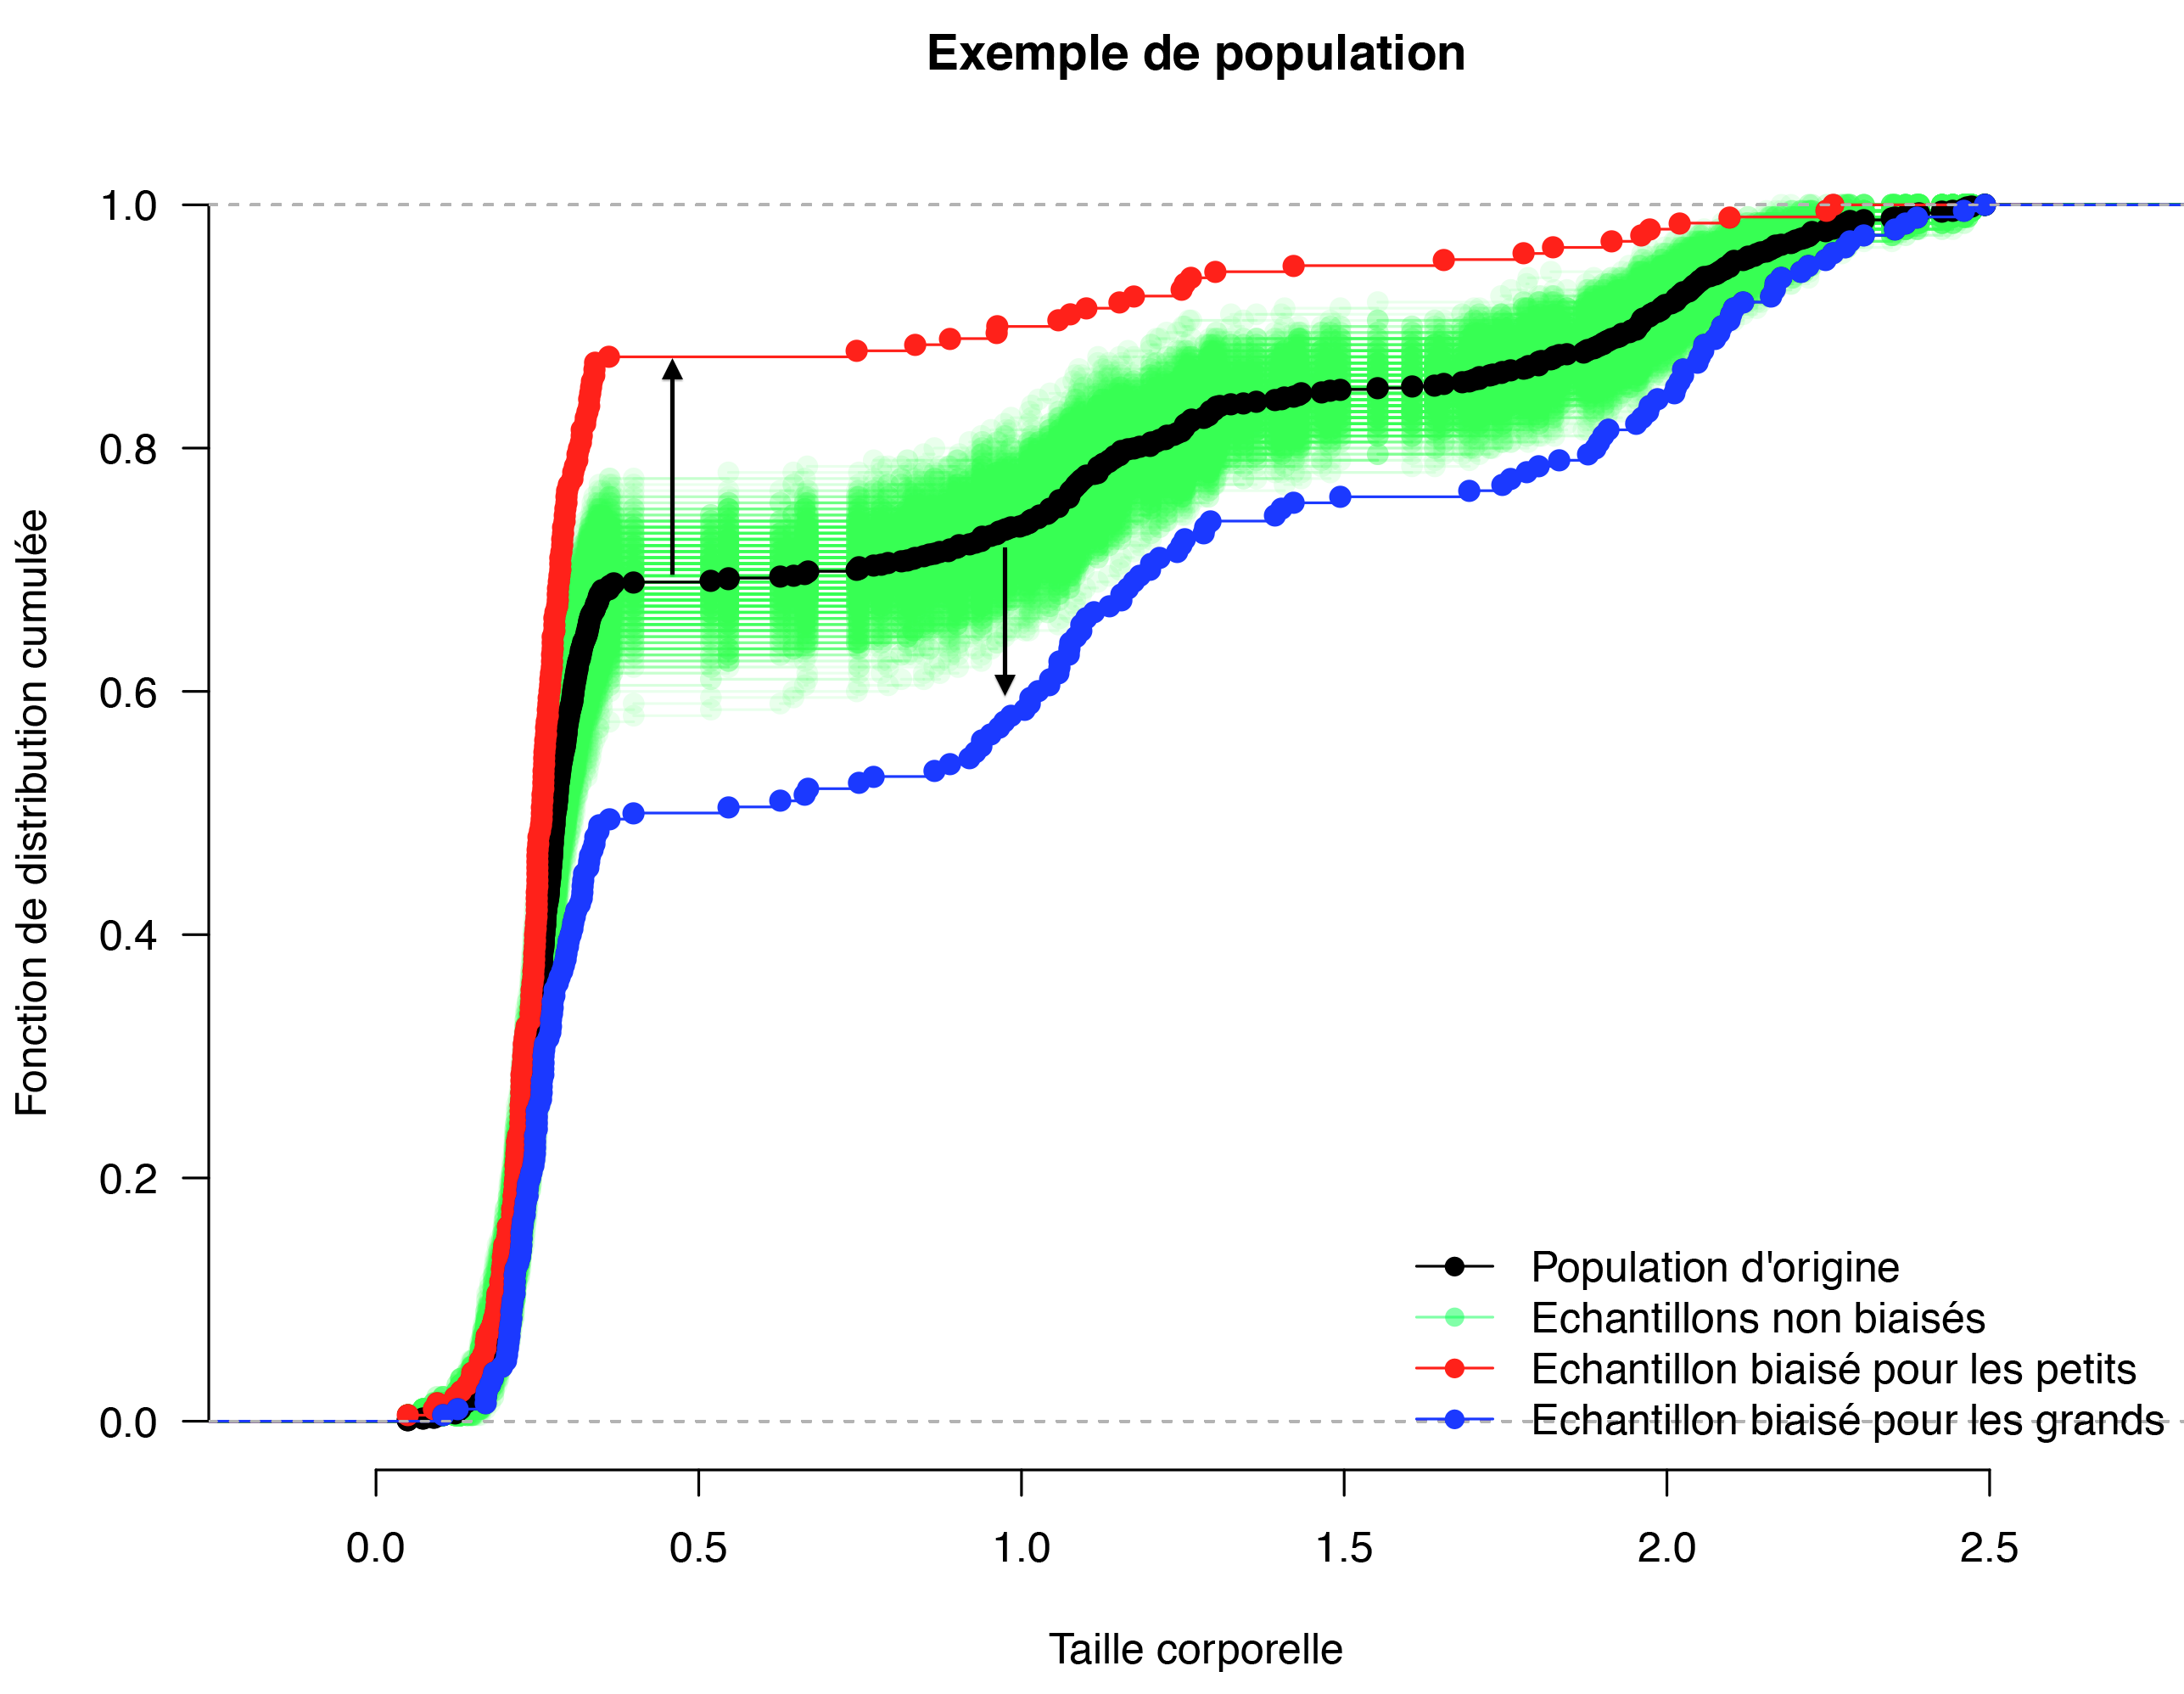
\includegraphics[width=0.66\textwidth]{1_CorpsDeThese/Resumes/Fig/SM02}
\caption[\lofimage{1_CorpsDeThese/Resumes/Fig/SM02}Comparaison des
distributions cumulées]{Exemple de comparaison des distributions cumulées entre
une population totale hypothétique (890 individus) et différents échantillons de
cette population (200 individus).
}
\label{fig:SM2}
\end{center}
\end{figure}

Les différences de distribution en taille des individus qui accèdent à la
ressource sont mesurées et comparées à la population originale en comparant les
fonctions de distribution cumulées de la taille (Figure \ref{fig:SM2}). Nous
utilisons les tests de Kolmogorov-Smirnov (KS) à deux échantillons afin de
tester la significativité de la différence et sa direction. Si la distribution cumulée
de la taille des individus accédant à la pastille est au-dessus de celle de la
population totale, cela signifie qu'il y a en proportion d'avantage de petits
individus accédant à la pastille de ressource que dans la population totale
(Figure \ref{fig:SM2}, échantillon rouge). A l'inverse, si la fonction de
distribution cumulée de la taille des individus accédant à la pastille est en
dessous de celle dans la population totale, cela signifie qu'en proportion, plus
d'individus de grande taille se trouvent sur la ressource que dans la population
totale (Figure \ref{fig:SM2}, échantillon bleu).

Les individus qui accèdent à la ressource représentent un sous-échantillon de la
population totale. Même si le test KS est significatif, nous avons vérifié que
cet échantillon est significativement différent d'un échantillon de même taille
tiré aléatoirement dans la population. Pour chaque population observée, nous
avons tiré aléatoirement $1000$ échantillons de même taille que celui des
individus accédant aux ressources afin de créer un intervalle de confiance des
échantillons aléatoires de la population totale (Figure \ref{fig:SM2},
échantillons verts). Si la distribution des individus accédant aux ressources
est en dehors de cet intervalle, cela confirme que le biais mesuré par le test KS
n'est pas dû au hasard.

% Afin d'avoir une mesure de ce biais et de sa direction, nous comparons la
% distance entre la distribution cumulée de la taille dans la population d'origine
% et la distribution moyenne de la taille des individus accédant à la ressource.
% La distance est calculée comme étant l'aire entre les deux courbes. La distance
% est soit absolue, il s'agit alors simplement de la mesure de l'aire entre les
% deux courbes, soit relative, il s'agit alors d'une aire positive si la
% distribution de l'échantillon est au dessus de celle de la distribution
% d'origine, négative si elle est en dessous. On peut alors tracer sur un graphe
% la distance relative en fonction de la distance absolue (\ref{fig:SM2}b). La
% position du point donne une indication de la direction et de l'intensité du
% biais.



\section{Résultats}

\subsection{Manipulation de la structure}

Les diagrammes structure-temps des populations témoins sont montrés figure
\ref{fig:SM3} et les populations manipulées sont présentées sur la Figure
\ref{fig:SM4}.

\begin{figure}[!ht]
\begin{center}
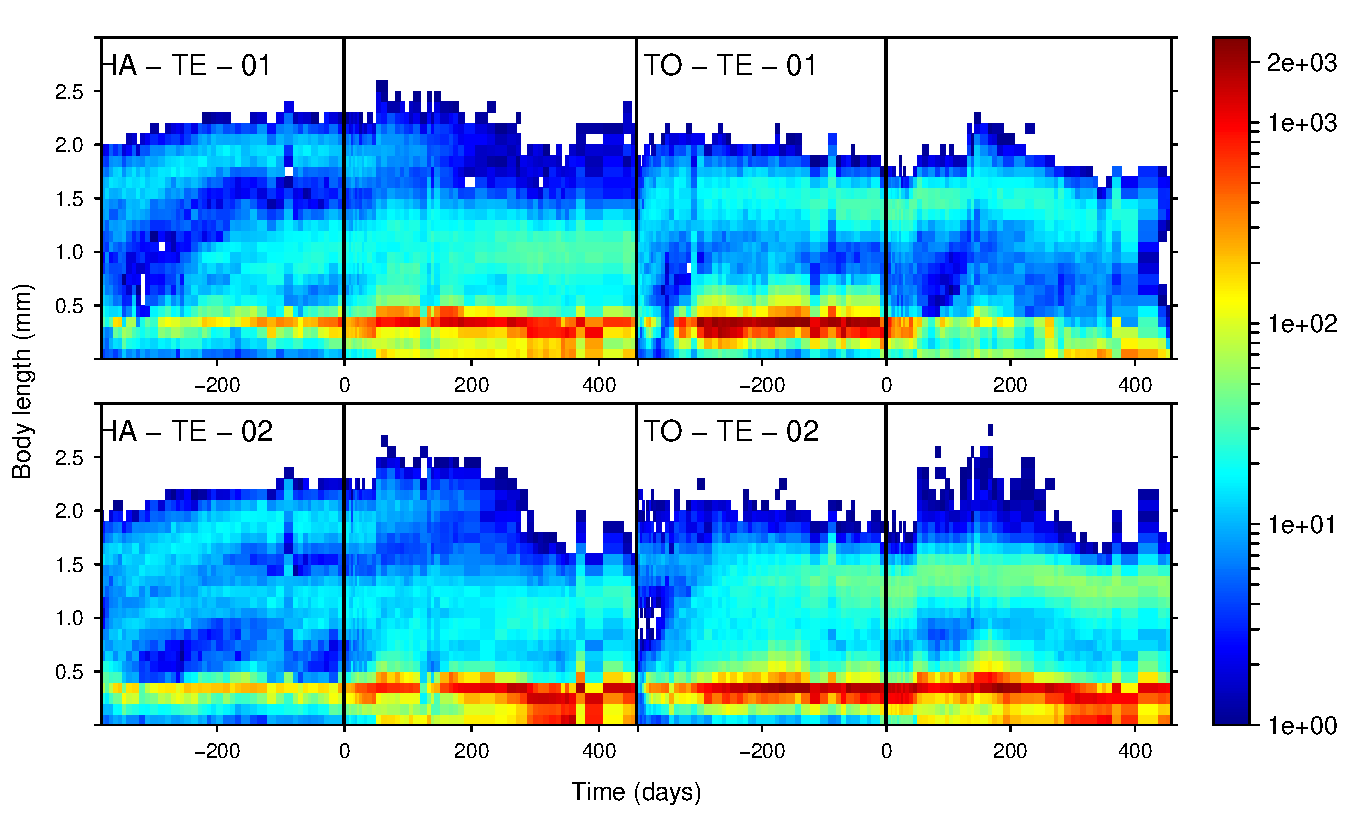
\includegraphics[width=1\textwidth]{1_CorpsDeThese/Resumes/Fig/SM04}
\caption[\lofimage{1_CorpsDeThese/Resumes/Fig/SM04}Population
témoins des clones HA et TO]{Population
témoins des clones HA et TO. La ligne vertical à la date 0 marque le moment où
les populations ont été manipulées.}
\label{fig:SM3}
\end{center}
\end{figure}

Dans les populations témoins, on constate que le changement de boite d'élevage
n'a pas eu d'effet immédiat sur les dynamiques des structures de populations. En
effet, on ne remarque pas de changement abrupt dans la structure de la
population au moment du transfert. Au contraire, les dynamiques observées
peuvent être comparées aux dynamiques présentées dans les Chapitre \ref{chap:sp}
(voir aussi Annexe \ref{Ann:SP}). Chez le clone HA, les deux populations témoins
sont trimodales au moment du transfert de boite d'élevage. Il semble que dans
les deux boites le mode des adultes les plus grands soit déjà décroissant au
moment du transfert et il s'éteint quelque temps après. Le temps de survie de ce
mode dans chacune des populations est de l'ordre de 500 jours, ce qui correspond
aux durées observées dans les populations non manipulées du Chapitre
\ref{chap:sp} (voir aussi Annexe \ref{Ann:SP}). Les deux populations TO montrent
également des dynamiques similaires aux populations non manipulées. On ne
constate pas de modification majeure dans la dynamique suite au transfert des
populations dans une nouvelle boite d'élevage.

\subsubsection{Traitements 1: Je - MG}

Dans ce traitement, la classe des juvéniles (Je) est isolée dans une boite alors
que les petits et grands adultes sont conservés ensemble et placés également
dans une nouvelle boite. Que ce soit pour le clone HA ou TO, on constate dans
les populations de juvéniles isolés le démarrage de la croissance d'une grande
partie des juvéniles dès le jour 0 (jour du transfert). Les ressources étant
apportées dans la même quantité qu'avant la manipulation, on observe l'effet du
relâchement de la compétition qui donne la possibilité aux juvéniles de grandir.
La cohorte qui démarre une croissance est très dense et conduit la structure de
la population vers une structure de type 1 (Chapitre \ref{chap:sp} et Annexe
\ref{Ann:SP}) avec des petits adultes en grande quantité et un grand nombre de
juvéniles. Dans ce traitement, les dynamiques des clones HA et TO sont très
semblables. En effet, le nombre de juvéniles qui maturent d'un coup est
suffisamment important pour empêcher HA d'exprimer sa capacité à produire des
adultes de grande taille.

\afterpage{%
    \clearpage% flush all other floats
    \ifodd\value{page}
    %\else% uncomment this else to get odd/even instead of even/odd
        \expandafter\afterpage% put it on the next page if this one is odd
    \fi
    {%
    \begin{figure}[p]
        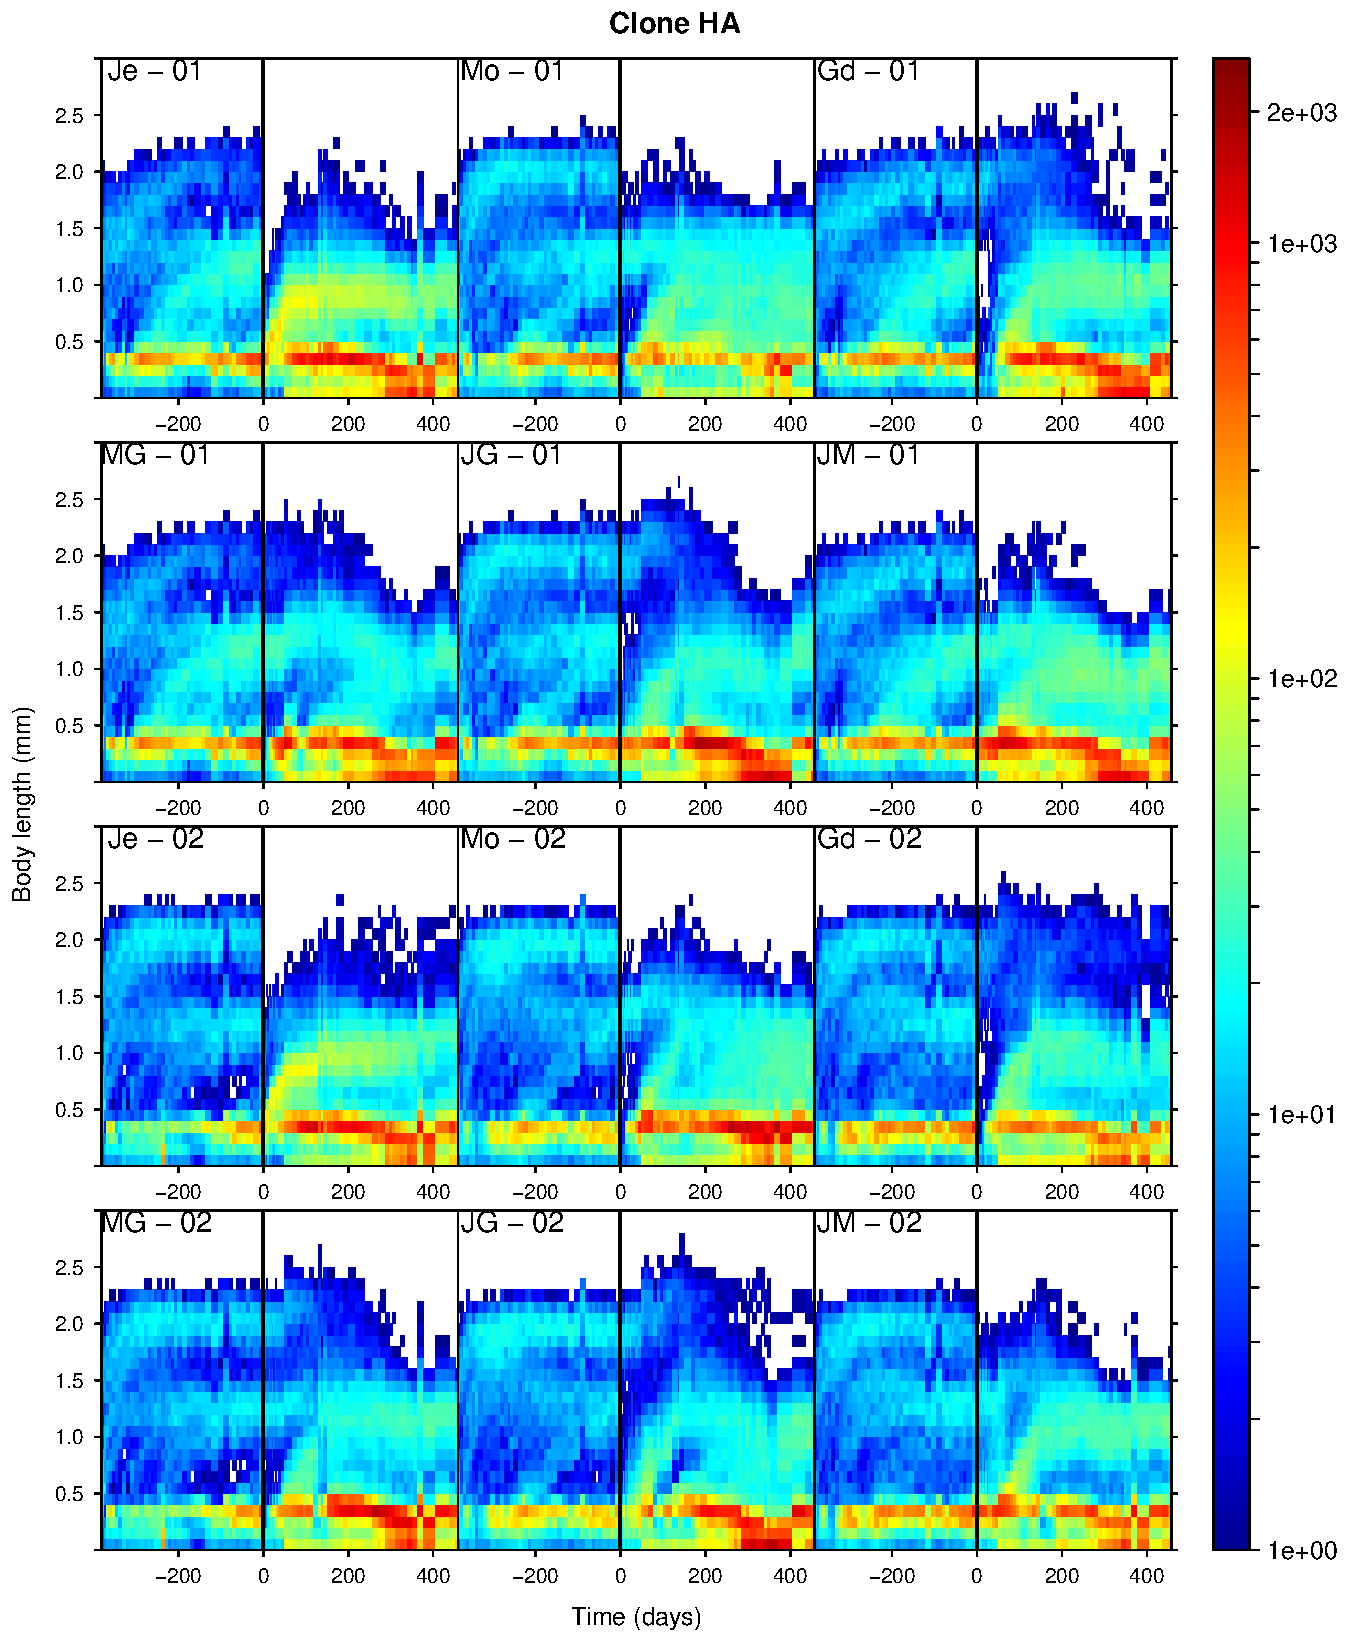
\includegraphics[width=\textwidth]{1_CorpsDeThese/Resumes/Fig/SM03a}
        \caption[\lofimage{1_CorpsDeThese/Resumes/Fig/SM03a}Diagrammes
        structure-temps des populations manipulées]{Diagrammes
        structure-temps des populations manipulées. La ligne vertical à la date 0 marque le moment où les populations ont été
        manipulées. Clone HA\ldots}\label{fig:SM4}
    \end{figure}
    \clearpage
    \begin{figure}[p]
		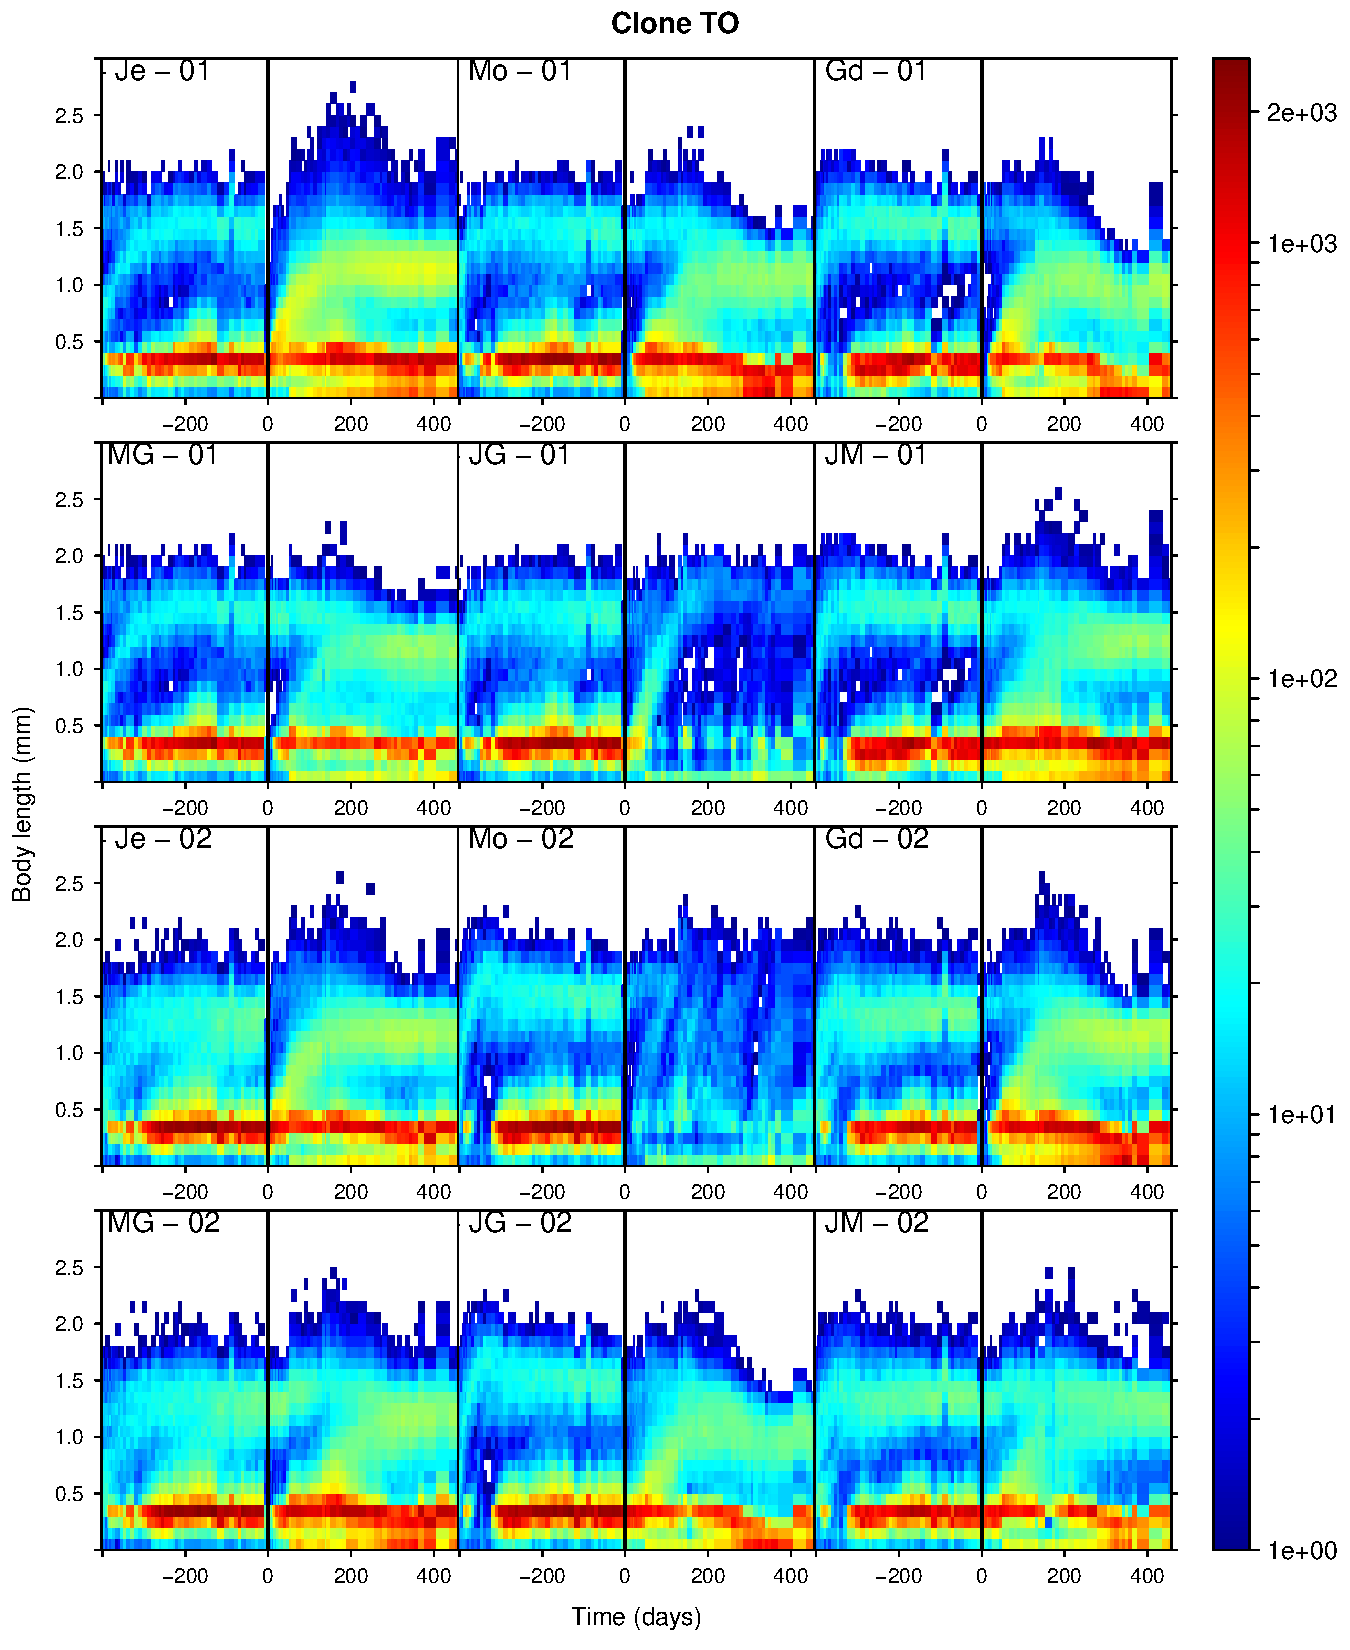
\includegraphics[width=\textwidth]{1_CorpsDeThese/Resumes/Fig/SM03b}
        \caption*{\ldots et Clone TO.}
    \end{figure}
    \clearpage
    }%
}



Dans les populations des adultes (MG), on constate chez HA que dès la
séparation les adultes reprennent également de la croissance. Ceci coïncide
également avec une disparition de la cohorte des adultes les plus grands. Cette
reprise de croissance semble montrer que malgré leurs faibles capacités
d'interférence, les juvéniles, de part leur grand nombre, exerce quand même une
pression de compétition par exploitation sur les adultes, limitant leur
possibilité de croissance. D'un point de vue de la dynamique de la structure,
dès la séparation, les adultes ont pondu et de nouvelles éclosions surviennent
après quelques semaines. On se retrouve alors de nouveau dans une situation
proche des structures de type 1 (Chapitre \ref{chap:sp} et Annexe \ref{Ann:SP}).
Ainsi, malgré le relâchement de la compétition par exploitation, les adultes les plus grands finissent par s'éteindre comme
dans les populations témoins, et ne sont pas remplacés. 

Chez le clone TO, la situation est similaire, avec un léger ajustement de la
taille immédiatement après la séparation de la population. Mais cet ajustement
s'accompagne de ponte très importantes et de nombreuses éclosions suivies de
la croissance d'une cohorte qui ramènent de nouveau les populations vers une
structure composée de petits adultes et d'un grand nombre de juvéniles.
Ainsi, le retrait des juvéniles n'a que peu d'effet car les adultes renouvellent très rapidement le
pool de juvéniles grâce à leur grande capacité de ponte. En quelques semaines,
les populations ont absorbé la perturbation et la dynamique semble peu affectée.
Il semble que ce soient les adultes de la population qui soient
responsable de la résilience de sa structure en taille: le retrait des juvéniles
modifie peu la dynamique de la structure, alors que le retrait de l'ensemble des
adultes a un effet important sur cette dynamique et peut faire basculer entre
différents types de structure. 

\subsubsection{Traitements 2: Mo - JG}

Dans ce traitement, les adultes de taille intermédiaire (Mo) sont isolés et les
juvéniles et les grands adultes (JG) sont conservés ensembles.

Chez les deux clones, l'isolation des adultes moyens (clone HA) ou de deux tiers
des adultes (clone TO) provoque une légère reprise de croissance accompagnée de
larges pontes et de la croissance d'une cohorte, qui ramène les populations dans
une structure semblable au traitement MG. Encore une fois, le retrait d'une
partie de la population relâche la compétition, ce qui explique la reprise de croissance,
mais celle-ci n'est pas suffisante comparée à la croissance des juvéniles pour
que les adultes HA atteignent les tailles du groupe de géant, ce qui ne permet
pas aux populations HA de retrouver une structure trimodale. Chez TO, la
deuxième population (TO Mo - 02) présente une réponse différente à la
perturbation. Lors du transfert des adultes moyens dans une nouvelle boite, il
semblerait qu'il y ait eu une forte mortalité et la population entre dans une
sorte de période cyclique avec des recrutements et remplacement des adultes
successifs. Ceci s'apparente d'avantage à une situation où les plus petits
individus dominent la population, ce qui pourrait s'expliquer par l'éclosion
rapide d'un grand nombre de juvéniles alors que peu d'adultes sont présents. 

Dans les populations JG, on constate là encore une reprise de croissance chez
les adultes restant, et des éclosions massives peu de temps après la séparation.
Chez HA, les adultes de grande taille meurent peu à peu et les populations
retournent à une distribution bimodale. Chez TO, on observe là encore deux cas
différents, dans le premier, une cohorte de petite densité parvient à grandir
jusqu'à une taille relativement importante, il y a alors relativement peu de
pontes, et la population se maintient avec une structure de type 2 (Chapitre
\ref{chap:sp} et Annexe \ref{Ann:SP}), alors que dans le second cas, on observe le
comportement classique avec un recrutement massif d'individus, et une population qui converge
vers une structure de type 1.

Ainsi, alors que le retrait des juvéniles avait relativement peu d'effet sur la
structure des populations comparé aux populations témoins, le retrait des
adultes de taille intermédiaire provoque une période transitoire un peu plus
longue qu'au par avant, voir un changement d'attracteur et la convergence vers
une structure et une dynamique très différente. 

\subsubsection{Traitements 3: Gd - JM}

Dans ce traitement, les juvéniles et les adultes de petite taille (clone HA) ou
les deux tiers des adultes (clone TO) sont conservés ensemble, le reste des
adultes (les grands pour HA et le tiers restant pour TO) est isolé. 

Dans les populations de grands adultes isolés (Gd), la réponse à la perturbation
est similaire à ce qui était observé pour les populations d'adultes
intermédiaires (Mo). En effet, la séparation des populations est suivie par une
période transitoire où les adultes restant grandissent légèrement et produisent
de nouvelles pontes. Lorsque ces pontes éclosent, une cohorte recrute
directement chez les adultes intermédiaires mais pas chez les plus grands. De
même pour TO, des cohortes très denses recrutent et atteignent rapidement la
taille adulte. 

Il est plus intéressant de noter que le retrait des adultes les plus grands des
populations HA  (JM 01 et 02) provoque également le recrutement d'une nouvelle
cohorte, mais plus dense que dans les traitements JG (où les adultes
intermédiaires sont retirés). Ainsi, bien que l'on retire moins d'individus
de la population (la cohorte d'adultes de grande taille est moins dense), le
fait de retirer les individus les plus grands des populations HA permet un
recrutement plus massif chez les juvéniles, ce qui signifie que la compétition
pour la ressource est retombé à un niveau plus bas que pour les traitements JG.
Chez TO, on n'observe pas ce phénomène car les traitements JM et JG diffèrent
par le nombre d'individus retirés des populations mais pas par la taille des
individus. Ainsi, en retirant le groupe G, on retire deux fois moins d'individus
que dans le groupe M, mais de la même taille. L'effet sur la compétition est
donc d'avantage lié au nombre d'individus retirés, plus qu'à la taille de ces
derniers. 

\subsubsection{En résumé}

Ces différents traitements semblent montrer que la présence d'adultes dans la
population affecte directement la capacité des juvéniles à grandir et arriver
à maturation. En effet, dès la suppression d'une partie des adultes, les
juvéniles présents dans la population se mettent immédiatement à grandir, et si
aucun juvénile n'est présent, les nouveaux nés démarrent également leur
croissance immédiatement. Cet effet des adultes sur la dynamique de la structure
des populations se manifeste au travers de deux facteurs, leur nombre et leur
taille. Si tous les adultes sont de même taille, le retrait d'une plus grande
quantité d'adultes permet à un plus grand nombre de juvéniles de recruter. Mais
ce qui est plus intéressant, c'est que si des adultes de taille différentes sont
présents, le retrait des adultes les plus grands, même s'ils sont moins nombreux
permet à d'avantage de juvéniles de grandir. Cela montre que la taille des
adultes joue un rôle direct sur la pression de compétition qu'ils imposent aux
juvéniles, ce qui est un argument qui soutient la compétition par
interférence comme mécanisme de régulation de la dynamique. 

\subsection{Observations comportementales}

Dans un second temps, nous nous sommes intéressés aux comportements
individuels d'accès à la ressource disponible. Les observations ont été
réalisées sur certaines des populations manipulées dans l'expérience précédente.
Ces observations comportementales et la mesure du biais de taille dans la capacité à accéder aux
ressources va nous permettre de confirmer le rôle de la compétition par
interférence.

\subsubsection{Exemple d'observation comportementale}

\begin{figure}[!ht]
\begin{center}
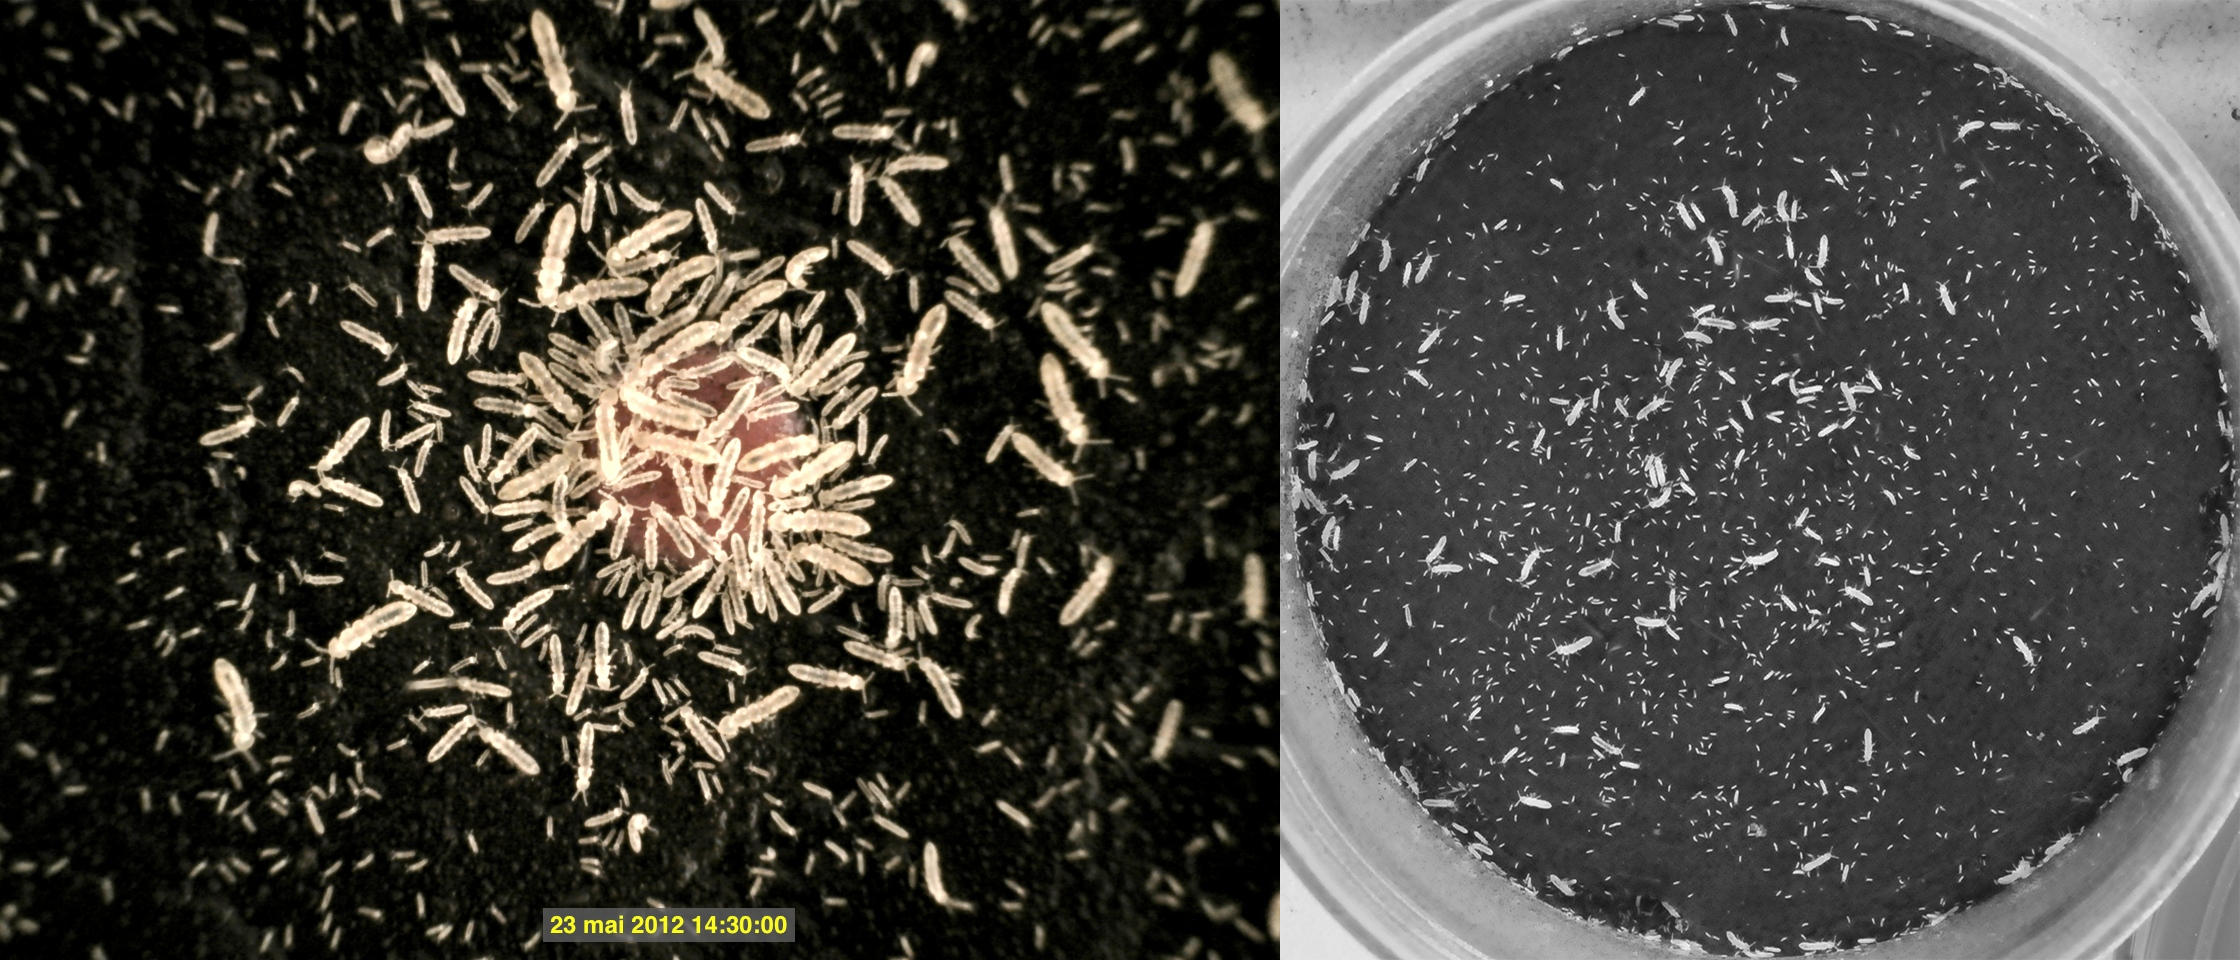
\includegraphics[width=1\textwidth]{1_CorpsDeThese/Resumes/Fig/SM05b}
\caption[\lofimage{1_CorpsDeThese/Resumes/Fig/SM05b}Cliché
d'observation de l'accès à la ressource]{Cliché
d'observation de l'accès à la ressource pour la population témoin HA-01 et
cliché de la population totale à une date proche.}
\label{fig:SM5}
\end{center}
\end{figure}

La Figure \ref{fig:SM5} montre un exemple de cliché pris au cours de
l'observation comportementale de l'accès aux ressources. Ce cliché a été pris
pour la population témoin HA 01. Bien que ce ne soit qu'un seul exemple de
cliché, cet exemple est très représentatif de ce qui a été observé dans toutes
les populations mesurées. On peut observer sur ce cliché une forte concentration
d'individus regroupés sur la pastille de nourriture (en rouge au centre) et des
individus plus dispersés aux alentours. Il est intéressant de constater la
différence de taille des individus sur ou aux abords de la pastille de ressource
comparée à la celle des individus plus éloignés et à l'ensemble des individus de
la population. Alors que les individus éloignés sont majoritairement des
juvéniles, les individus les plus gros présents sur ce cliché sont tous sur la
pastille de ressource ou dans ses environs proches.
Ceci est observé alors même qu'en nombre d'individus, cette population est
largement dominée par les juvéniles. Si l'accès à la ressource était indépendant
de la taille, on s'attendrait donc à avoir davantage de juvéniles présents sur
la pastille que de grands individus. Il y a donc un biais de taille corporel
manifeste dans l'accès à la ressource.

\begin{figure}[!ht]
\begin{center}
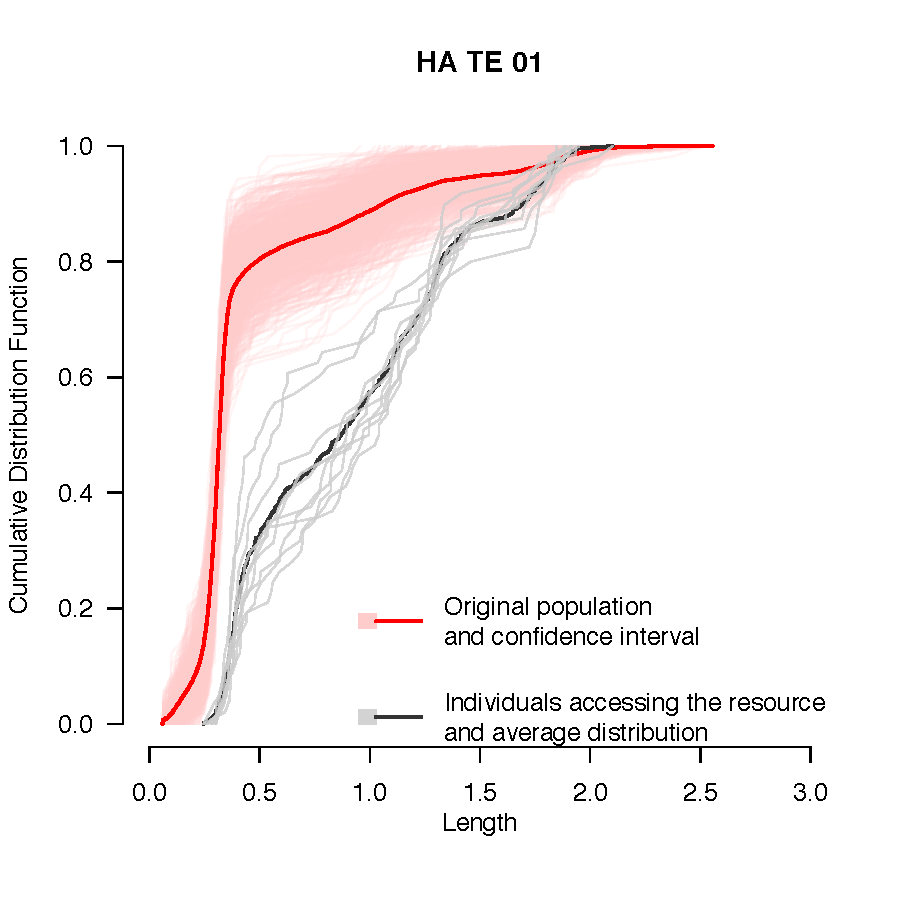
\includegraphics[width=0.75\textwidth]{1_CorpsDeThese/Resumes/Fig/SM06}
\caption[\lofimage{1_CorpsDeThese/Resumes/Fig/SM06}Mesure du biais
d'accès aux ressources]{Mesure du biais
d'accès aux ressources pour la population témoin HA 01. Test de
Kolmogorov-Smirnov de comparaison de deux échantillons: gris en dessous du
rouge: $p<10^{-10}$.}
\label{fig:SM6}
\end{center}
\end{figure}

Le cliché présenté en Figure \ref{fig:SM5} fait partie d'une série de 10 clichés
de la même population à 15 minutes d'intervalle. La Figure \ref{fig:SM6}
présente les fonctions de distribution cumulées de la population totale (rouge),
des individus accédant à la ressource sur chacun des clichés (gris clair), de la
moyenne des individus accédant à la ressource (gris foncé), et de 1000
échantillons aléatoires de même taille que la distribution moyenne des individus
accédant à la ressource (rouge clair). On constate que les dix distributions en
gris sont systématiquement en dessous de la distribution dans la population entière. Qui
plus est, elles sont également systématiquement en dehors de l'intervalle des
sous échantillons aléatoires. Le test de comparaison des distributions,
effectué avec la distribution moyenne sur la pastille est également extrêmement
significatif.
Cela nous permet d'affirmer qu'il y a un biais significatif en faveur des
individus les plus grands de la population dans l'accès à la ressource. En
effet, alors que $80\%$ des individus de la population mesurent moins de
$0.5mm$, ils ne représentent qu'un tiers des individus présents sur ou aux
abords de la pastille de nourriture. De plus, $13\%$ des individus sur la
ressource mesurent plus de $1.6mm$ alors qu'ils représentent moins de $5\%$ de
la population totale. Enfin, $50\%$ des individus présents sur la pastille ont
une taille entre $0.45$ et $1.35mm$ alors que cette classe de taille ne
constitue que $15\%$ de la population totale.

\subsubsection{Mesure du biais d'accès aux ressources}

La mesure du biais par comparaison des distributions cumulées a été réalisée sur
10 populations. La Figure \ref{fig:SM7} présente les distributions cumulées des
neufs autres séries d'observation.
On constate que dans tous les cas il existe un biais en faveur des individus les
plus grands pour l'accès à la ressource. On constate également que même dans les
populations où le nombre de grands individus est relativement important, telle
que TO TE 01, le biais reste significatif avec une large sous représentation des
$40\%$ d'individus de moins de $0.5mm$.

On remarque encore que même dans les populations où les juvéniles représentent
plus de $80\%$ de la population totale (HA JM 01, HA JM 02, HA TE 02, TO MG 02),
on ne comptabilise sur la ressource jamais plus de $50\%$ d'individus de moins
de $0.6mm$. Sur l'ensemble des cas étudiés, les $10\%$ les plus grands des
individus de la population totale représentent jusqu'à plus de $50\%$ des
individus mesurés sur les ressources, et généralement autour de$20\%$.

\begin{figure}[!ht]
\begin{center}
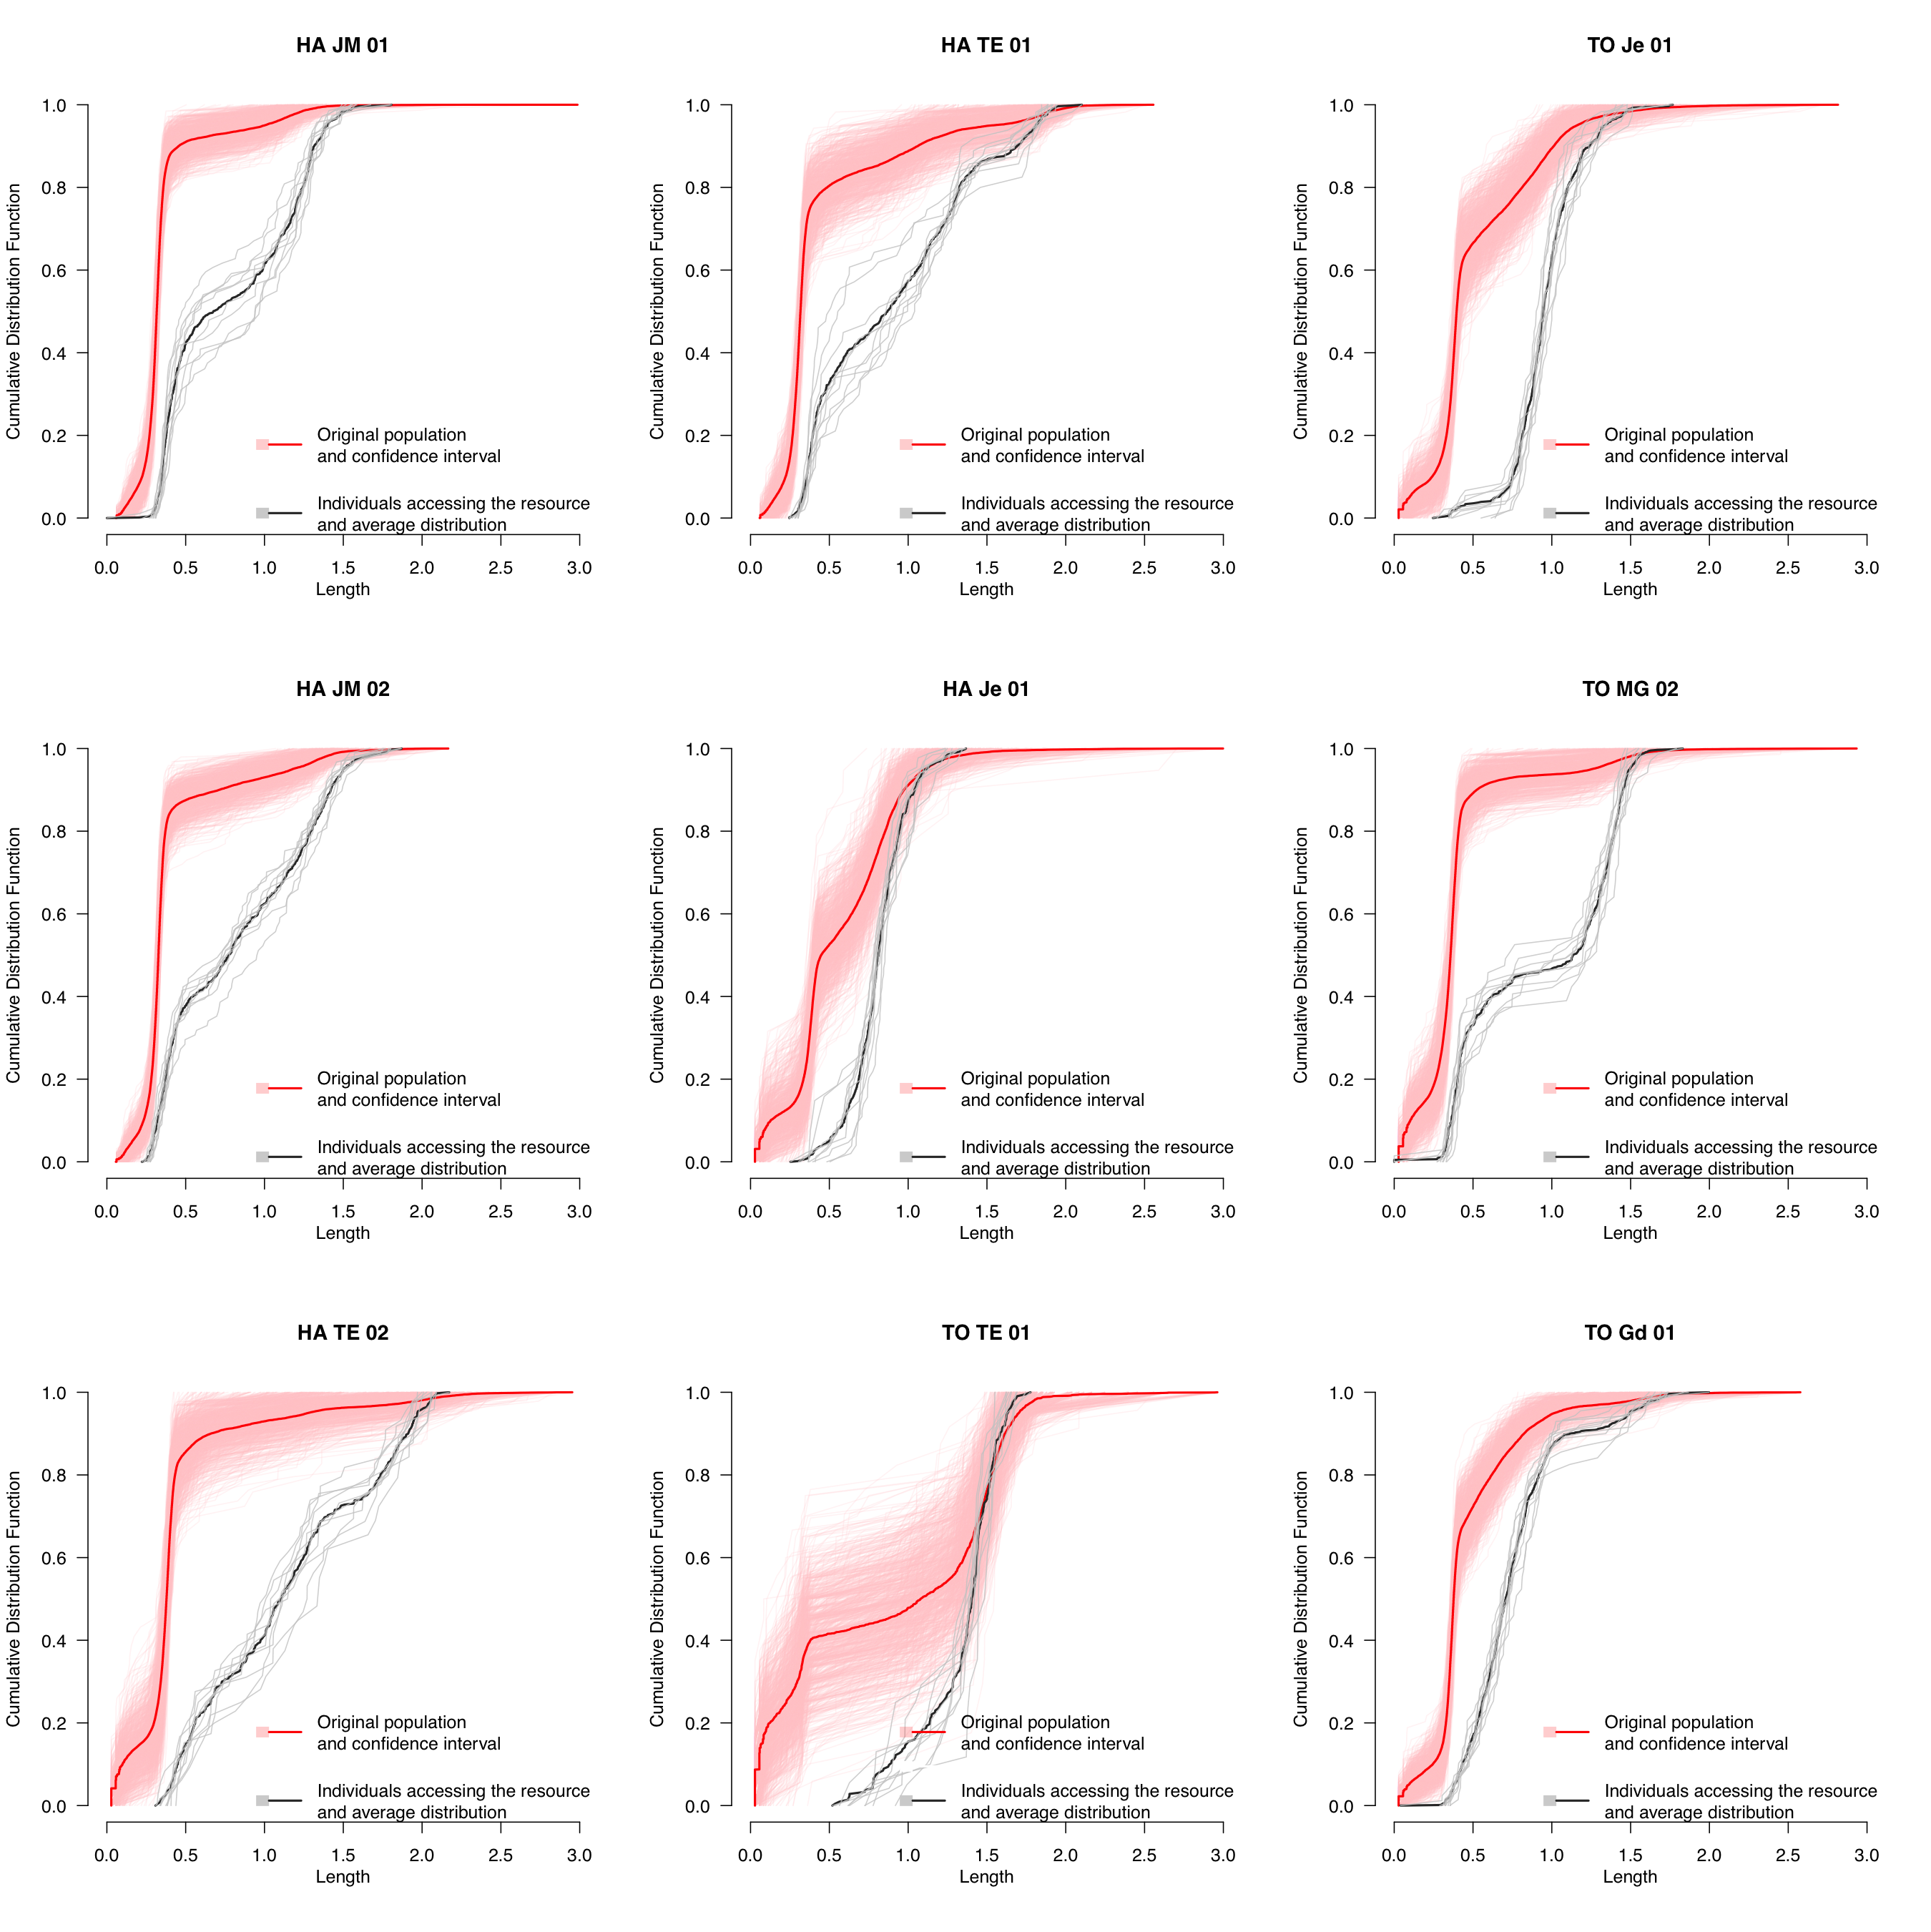
\includegraphics[width=1\textwidth]{1_CorpsDeThese/Resumes/Fig/SM07}
\caption[\lofimage{1_CorpsDeThese/Resumes/Fig/SM07}Mesures du biais
d'accès aux ressources]{Mesures du biais
d'accès aux ressources pour 9 autres populations. Tests KS: $p \ll 0.01$}
\label{fig:SM7}
\end{center}
\end{figure}

Les biais en faveur des grands individus dans l'accès à la ressource semblent
donc être systématiques, quelle que soit la population étudiée. Nous avons
utilisé dans ces observations des populations dont la structuration en taille était
différente.
Ainsi, même avec très peu de grands individus dans la population, ceux-ci sont
très largement sur-représentés lors des comptages sur les pastilles. Il semble
donc que la capacité des individus de grande taille à dominer la ressource soit
commune à nos deux clones, et ne dépende que peu des conditions de densité de la
population. Lors de la prise des clichés servant de base à ces mesures, nous
avons également pu identifier en temps réel des interactions
compétitives entre individus: des individus se
mettaient à tourner rapidement en rond lorsque d'autre s'approchaient de trop prêt, provoquant leur fuite. Ces comportements étaient
particulièrement visibles chez les individus les plus grands, faisant fuir
rapidement les plus petits. Ainsi, la
domination des plus grands individus sur la ressource passe notamment par des
comportements consistant à chasser les individus plus faibles de leur
environnement direct, empêchant les fuyards d'accéder à la ressource. Ce
comportement répond à notre définition précédente de la compétition par
interférence (Chapitres \ref{chap:method} et \ref{chap:amnat}, et Annexe
\ref{An:AmNat}).

\section{Discussion}

Au cours de cette étude, nous avons analysé la réponse de la structure en taille
de populations de collemboles à des perturbations. Plusieurs perturbations ont
été appliquées aux deux clones étudiés jusque là, HA et TO. Ces perturbations
ont consisté à manipuler la structure en taille de la population pour observer
l'établissement d'un nouvel équilibre en fonction des nouvelles conditions
imposées. 

Nous avons également réalisé une série d'observations des
comportements individuels d'accès aux ressources. Ces observations nous ont
permis de mettre en évidence un biais systématique dans l'accès à la ressource
en faveur des individus les plus grands de la population. 

\subsection{Stabilité et résilience des différentes structures en taille}

Au cours de la première expérience, nous avons manipulé la structure de
plusieurs populations des clones HA et TO. Les différentes manipulations
réalisées ont permis de tester la stabilité des différents attracteurs décrits
dans le Chapitre \ref{chap:sp}. En effet, les huit populations HA utilisées
dans l'étude étaient toutes dans une structure de type 4 au moment de la
perturbation, alors que les populations TO étaient dans des structures de type 1
ou 2. Nous avions déjà constaté que les structures de type 4 n'étaient stable
que le temps de survie des adultes les plus grands; une fois disparus,
ces derniers n'étaient pas remplacés et les populations convergeaient vers
différentes structures. Ceci est encore confirmé par nos populations HA témoins,
en effet, les adultes les plus grands survivent après le changement de boite
d'élevage mais meurent de vieillesse après quelques centaines de jours (voir
\autocites{mallard2013b} pour plus d'informations sur le vieillissement).
La structure observée subit alors le même type de transition que les populations présentées
dans le Chapitre \ref{chap:sp} (voir aussi Annexe \ref{Ann:SP}). De plus,
lorsque les adultes les plus grands sont retirés des populations, ils ne sont pas remplacés malgré une légère
croissance des adultes de taille intermédiaire. A la place, une cohorte de
juvéniles parvient à grandir et rejoint les adultes intermédiaires, augmentant
la compétition au sein de cette classe, ce qui empêche une croissance vers les
très grandes tailles. Enfin, lorsque l'on enlève les juvéniles ou les adultes
de taille intermédiaire, les plus grands parviennent à se maintenir quelques
temps après perturbation mais ne sont pas remplacés après leur mort. Cette
structure trimodale est donc stable localement, mais le bassin d'attraction est
trop petit pour permettre de l'atteindre, à part dans des conditions très
particulières telles que décrites dans le Chapitre \ref{chap:sp} (voir aussi
Annexe \ref{Ann:SP}).

A l'inverse, la plupart des populations dont la structure a été modifiée au
moment de la manipulation convergent vers une structure avec un grand nombre de
juvéniles, et des adultes plutôt petits et en assez forte densité. Cette
structure, similaire aux structures de type 1, semble donc avoir un bassin
d'attraction plus large que les autres car elle est atteinte quel que soit la
manipulation effectuée sur la structure. Cette structure est généralement
atteinte lorsque beaucoup de juvéniles grandissent et atteignent la maturité en
même temps. Au cours de nos différentes manipulations, soit des juvéniles
étaient présents et pouvaient grandir dès que la pression de compétition était
relâchée par le retrait de tout ou partie des adultes, soit seul des adultes
étaient gardés, mais ils se sont alors massivement reproduits et à cause d'une
faible compétition, une large cohorte de juvénile a pu rapidement commencer à
grandir et atteindre la maturité. 

On constate également que le temps nécessaire à la stabilisation d'une nouvelle
structure semble dépendre principalement de la présence ou de l'absence des
adultes. En effet, les populations les plus rapides à atteindre un équilibre
sont celles dont tous les adultes ont été prélevés (2 à 3 semaines).
A l'inverse, les plus lentes sont celles dont seuls les juvéniles ont été
prélevés ($>200$ jours). En diminuant la possibilité des juvéniles d'accéder à
la ressource, les adultes acquièrent une longue survie, ce qui fait d'eux une
force stabilisatrice de la structure, mais en ralentissant la capacité de
grandir des juvéniles, cela ralentie également la possibilité pour la population
de se remettre d'une perturbation et notamment du prélèvement de ses juvéniles.

\subsection{Compétition par interférence}

L'impact du retrait des adultes d'une population sur la reprise de croissance
des juvéniles, ainsi que le biais dans l'accès aux ressources en faveur des
individus les plus grands viennent confirmer l'hypothèse de la compétition par
interférence comme force régulatrice de la dynamique de nos populations de
collemboles. Cette interférence s'exprime principalement via des comportements
individuels lors de l'accès à la ressource. En effet, les individus ont tendance
à chasser leurs voisins lorsqu'ils sont trop proches. Au cours de cette
opération, les individus les plus grands parviennent à chasser la plupart de
leurs voisins alors que les plus petits ne les affectent pas. Au contraire, les plus petits
ont davantage tendance à fuir, et limitent ainsi leur accès à la ressource. De
ce fait, la présence, même en faible densité, d'individus très grands affecte
fortement la dynamique de la structure comme proposé par notre étude théorique
du Chapitre \ref{chap:amnat} (voir aussi Annexe \ref{An:AmNat}). En monopolisant
la ressource, ils bloquent la croissance des individus plus petits, et une nouvelle cohorte de juvénile ne
parvient à grandir que lorsque les adultes les plus grands ont disparu, comme
observé dans les premières expériences présentées ici, et dans le Chapitre
\ref{chap:sp} (voir aussi Annexe \ref{Ann:SP}).

En revanche, contrairement a ce qui est prédit par le modèle, la disparition
ou le retrait de la cohorte des individus les plus grands ne provoque pas sont
remplacement, mais plutôt un changement de dynamique car lors de cette
disparition, beaucoup de juvéniles se mettent à grandir en une fois, ce qui
modifie fortement les rapports de compétition entre les différentes cohortes et
au sein de chacune.

De plus, les résultats de ces expériences montrent également que la compétition
par exploitation continue de jouer un rôle dans la régulation des populations.
En effet, la suppression de l'ensemble des juvéniles, les individus les plus
compétitifs par exploitation, affecte les adultes, qui sont alors capables de
reprendre leur croissance jusqu'à l'éclosion de nouvelles cohortes de juvéniles.

\section{En conclusion}

Cette série d'expérience a permis de confirmer le rôle
prépondérant que jouent les adultes dans la régulation de la dynamique des
populations structurées de Collembole. Mais elle a également apporté des
arguments montrant l'existence d'une régulation par la compétition par
exploitation. Les deux mécanismes semblent donc intimement liés, et c'est
l'équilibre entre les deux qui conduit aux dynamiques observées dans le Chapitre
\ref{chap:sp} (voir aussi Annexe \ref{Ann:SP}). Un changement brutal de cet
équilibre en prélevant une partie de la population, diminuant rapidement l'impact de la compétition par interférence
(en retirant les adultes) ou par exploitation (en retirant les juvéniles)
affecte la population en la conduisant généralement vers un nouvel équilibre de
structure. 

L'équilibre entre compétition par interférence et compétition par exploitation
dans la régulation des populations structurées dépend de la structure de la
population elle même, mais est également susceptible de dépendre des conditions
environnementales. La température est un élément connu pour son impact sur la
taille des individus, et est donc susceptible d'affecter cet équilibre en venant
non seulement modifier les trajectoires d'histoire de vie individuelles, mais
également les interactions entre les individus et les mécanismes de densité
dépendance. Les interactions entre mécanismes de compétition et effets
de la température seront l'objet du chapitre suivant. 



\chapter{Interactions entre compétition intraspécifique et température dans la
régulation des populations structurées}
\chaptermark{Compétition intraspécifique et température}
\label{chap:fip}

\vspace{2cm}
\begin{Spacing}{1}
\texttt{
Mallard, François, Vincent Le Bourlot, Christie Le Coeur, Monique Avnaim, David
Claessen and Thomas Tully, "From individuals to populations: \\intraspecific
competition breaks the temperature-size rule"\\
soumis à Journal of Animal Ecology}
\end{Spacing}
Voir Annexe \ref{Ann:fip}.
\vspace{2cm}


\lettrine[lines=3]{A}{u cours} des trois chapitres précédents, nous avons étudié
le rôle des mécanismes de compétition intraspécifiques sur la dynamique de
populations structurées de collemboles \textit{Folsomia candida} d'un point de vu théorique
et empirique. Ces études nous ont permis en particulier de mieux appréhender
l'impact de différents niveaux de compétition par interférence dans la
dynamique temporelle de la structure des populations. Cependant, ces études ont
été réalisées dans une seule condition environnementale. Or, comme nous
l'avons déjà expliqué, l'environnement, et en particulier la température, peut
avoir un impact à la fois sur les individus et les populations. 

En effet, des températures différentes affectent directement les taux
physiologiques (métabolisme, consommation, respiration,\ldots), ce qui a des
conséquences démographiques via des changements dans les cycles de vie
\autocites{gillooly2002a,le-galliard2012a}. Des changements de température
provoquent aussi de la plasticité phénotypique chez les individus en modifiant
par exemple l'allocation des ressources à la croissance ou à la reproduction
\autocites{liefting2010temperature,gutteling2007mapping}. Ceci résulte dans la
règle dite ``taille-température'' qui prédit une taille plus grande des
individus dans des environnements plus froids
\autocites{atkinson1994a,atkinson1996a,angilletta2009a}. Enfin, la température
peut avoir un effet sur les comportements individuels comme l'activité, la
dispersion ou le choix de l'habitat
\autocites{atacho2013a,bonte2008thermal,vanbeest2012temperature}.

L'approche classique de l'étude de l'influence de la température sur les
phénotypes consiste à mesurer des normes de réaction \autocites{woltereck1909a}.
Ces mesures sont généralement réalisées sur des individus isolés ou sur de
petites cohortes élevées au laboratoire dans différentes conditions de
température. Ces analyses apportent beaucoup d'informations sur les effets au
niveau de l'individu mais laissent de côté les conséquences de ces effets aux
niveaux des populations et des communautés. 

Dans ce chapitre, nous nous demandons a quel point les normes de réactions
mesurées au niveau individuel permettent des inférences sur la dynamique des
populations. Nous cherchons à comprendre comment les effets directs de la
température sur les traits d'histoire de vie individuels sont modulés par les
interactions entre individus et les rétroactions démographiques.
Les effets d'une augmentation de la température sur la compétition
inter-spécifique ont déjà été démontrés, provoquant notamment une augmentation
de la compétition par exploitation \autocites{ohlberger2011a}. Mais le cas de la
compétition intra-spécifique reste peu clair, et les effets sur la compétition par
interférence peuvent être différents de l'exploitation. L'interaction entre
les deux mécanismes, couplée aux effets directes de la température sur les individus,
rendent l'impact de la température sur les dynamiques des populations
structurées difficile à prévoir. Pour y parvenir, nous avons mesuré les normes de réaction
individuelles des taux de croissance et des tailles à maturité et tailles
asymptotiques dans quatre conditions de température, $11$, $16$, $21$ et
$26\degres$C. Nous avons également effectué des mesures de taux de croissance de
cohortes et de taille des cohortes adultes dans des populations élevées aux même
températures. Nous avons ainsi pu comparer les réponses à la température dans
deux conditions démographiques contrastées et en déduire l'importance de la
compétition intra-spécifique dans la réponse des populations à la température.

\section{Éléments de méthodologie}

\subsection{Conditions d'élevage et mesures}

Comme dans les expériences précédentes, les conditions d'élevage et les méthodes
de mesure de la taille individuelle et de la structure des populations suivent
les descriptions données dans le Chapitre \ref{chap:method}.

\subsubsection{Individus isolés}

Les nouveau-nés sont isolés immédiatement après la naissance et sont nourris
\textit{ad libitum} pendant toute leur vie. Les individus ont été placés
aléatoirement à une des quatre températures de notre intervalle ($11$, $16$, $21$ et
$26\degres$C). La taille corporelle est mesurée pour chaque individu trois fois
par semaine pendant dix semaines, puis une fois par semaine. Afin de déterminer
la maturation des individus, les boites d'élevage sont régulièrement inspectées
pour rechercher des pontes. La croissance des individus est ensuite modélisée
\ref{fig:FIP1} et Annexe Figure \ref{Fig5-S1}).
Le taux de croissance maximal moyen et la taille asymptotique sont estimés par des modèles
de moindre-carrés non linéaires ajustés séparément pour chacune des trajectoires
de croissance \autocites{pinheiro2000a}. Les effets fixes du clone et de la
température (prise comme variable catégorielle) sur le taux de croissance
maximal et la taille asymptotique ont été testés à l'aide de modèles linéaires
et de test de Fisher.

\begin{figure}[!ht]
\begin{center}
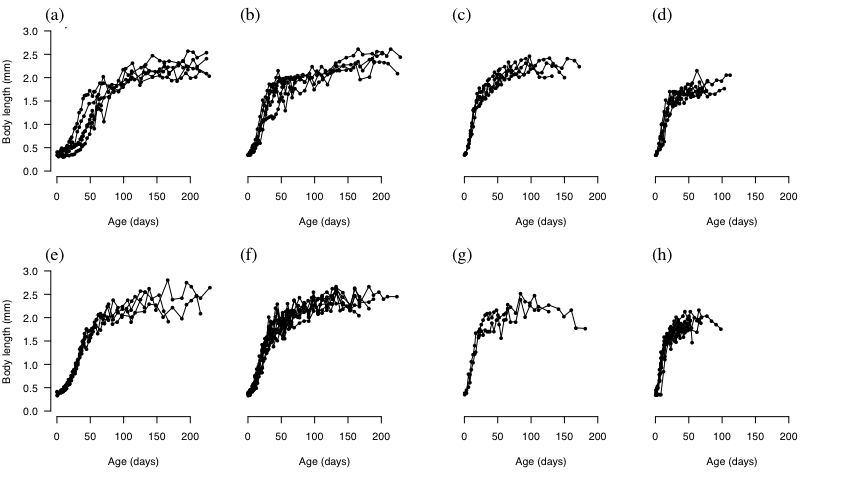
\includegraphics[width=\textwidth]{1_CorpsDeThese/Resumes/Fig/FIP01}
\caption[\lofimage{1_CorpsDeThese/Resumes/Fig/FIP01}Trajectoires de croissance
individuelles]{Trajectoires de croissance individuelles pour les clones HA
(a-d) et TO (e-h) à $11$ (a et e), 16 (b et f), 21 (c et g) et
$26\degres$C (d et h).}
\label{fig:FIP1}
\end{center}
\end{figure}


\subsubsection{Mesures de taille et de croissance dans les populations}

Pour les mesures de normes de réactions en contexte de population, quatre
populations ont été démarrées pour chaque température, excepté $21\degres$C où
les 28 populations présentées dans le Chapitre \ref{chap:sp} sont utilisées. La
structure des populations a été mesurée une fois par semaine pendant plus d'un
an. Les traits d'histoire de vie (taux de croissance des juvéniles et taille
adulte) ont été extraits des données grâce à la représentation en diagramme
structure-temps et aux outils annexes présentés dans le Chapitre
\ref{chap:method} Section \ref{sec:stdiag} (voir aussi Annexe \ref{Chap:STDiag}). 

Les taux de croissances juvéniles ont été mesurés sur des cohortes suffisamment
visibles sur les diagrammes et atteignant le groupe d'adultes (Figure
\ref{fig:FIP2} et Annexe Figure \ref{Fig5-S3}).
Le taux de croissance est estimé par la pente de la taille moyenne dans les cohortes au
cours du temps. La taille asymptotique des adultes est mesurée comme la taille
moyenne du groupe d'adultes une fois que la cohorte a totalement fusionné avec
les adultes déjà présents, ou quand sa taille moyenne se stabilise. La structure
de la population au moment de chaque mesure nous permet d'en connaître les
conditions démographiques (densité de juvéniles, d'adultes,\ldots). Les
individus sont considérés adultes lorsque leur taille excède $0.8mm$.

\subsubsection{Séparer les effets température et densité dépendance}

Dans nos populations, les changements dans les trais d'histoire de vie et les
taux démographiques peuvent être attribués à des effets directs de la
température sur les individus, à des effets directs des mécanismes de densité dépendance, ou
à une interaction entre les deux. Afin de pouvoir analyser les effets de la
densité dépendance (éventuellement en interaction avec la température) tout en
contrôlant pour les effets directs de la température, nous avons construit deux
indicateurs qui comparent les traits mesurés dans les populations aux mesures
faites sur les individus isolés. 

Pour analyser les différents effets sur le taux de croissance, nous avons
utilisé des modèles linéaires expliquant le rapport des taux de croissance dans
les populations sur les taux maximums moyens mesurés chez les individus isolés.
Nous appelons cet indicateur le ``\textbf{taux de croissance relatif en
population}''. Les variables explicatives que nous avons considérées sont le
logarithme du nombre d'adultes, la température, la lignée clonale et les
interactions entre les trois variables. 

\begin{figure}[H]
\begin{center}
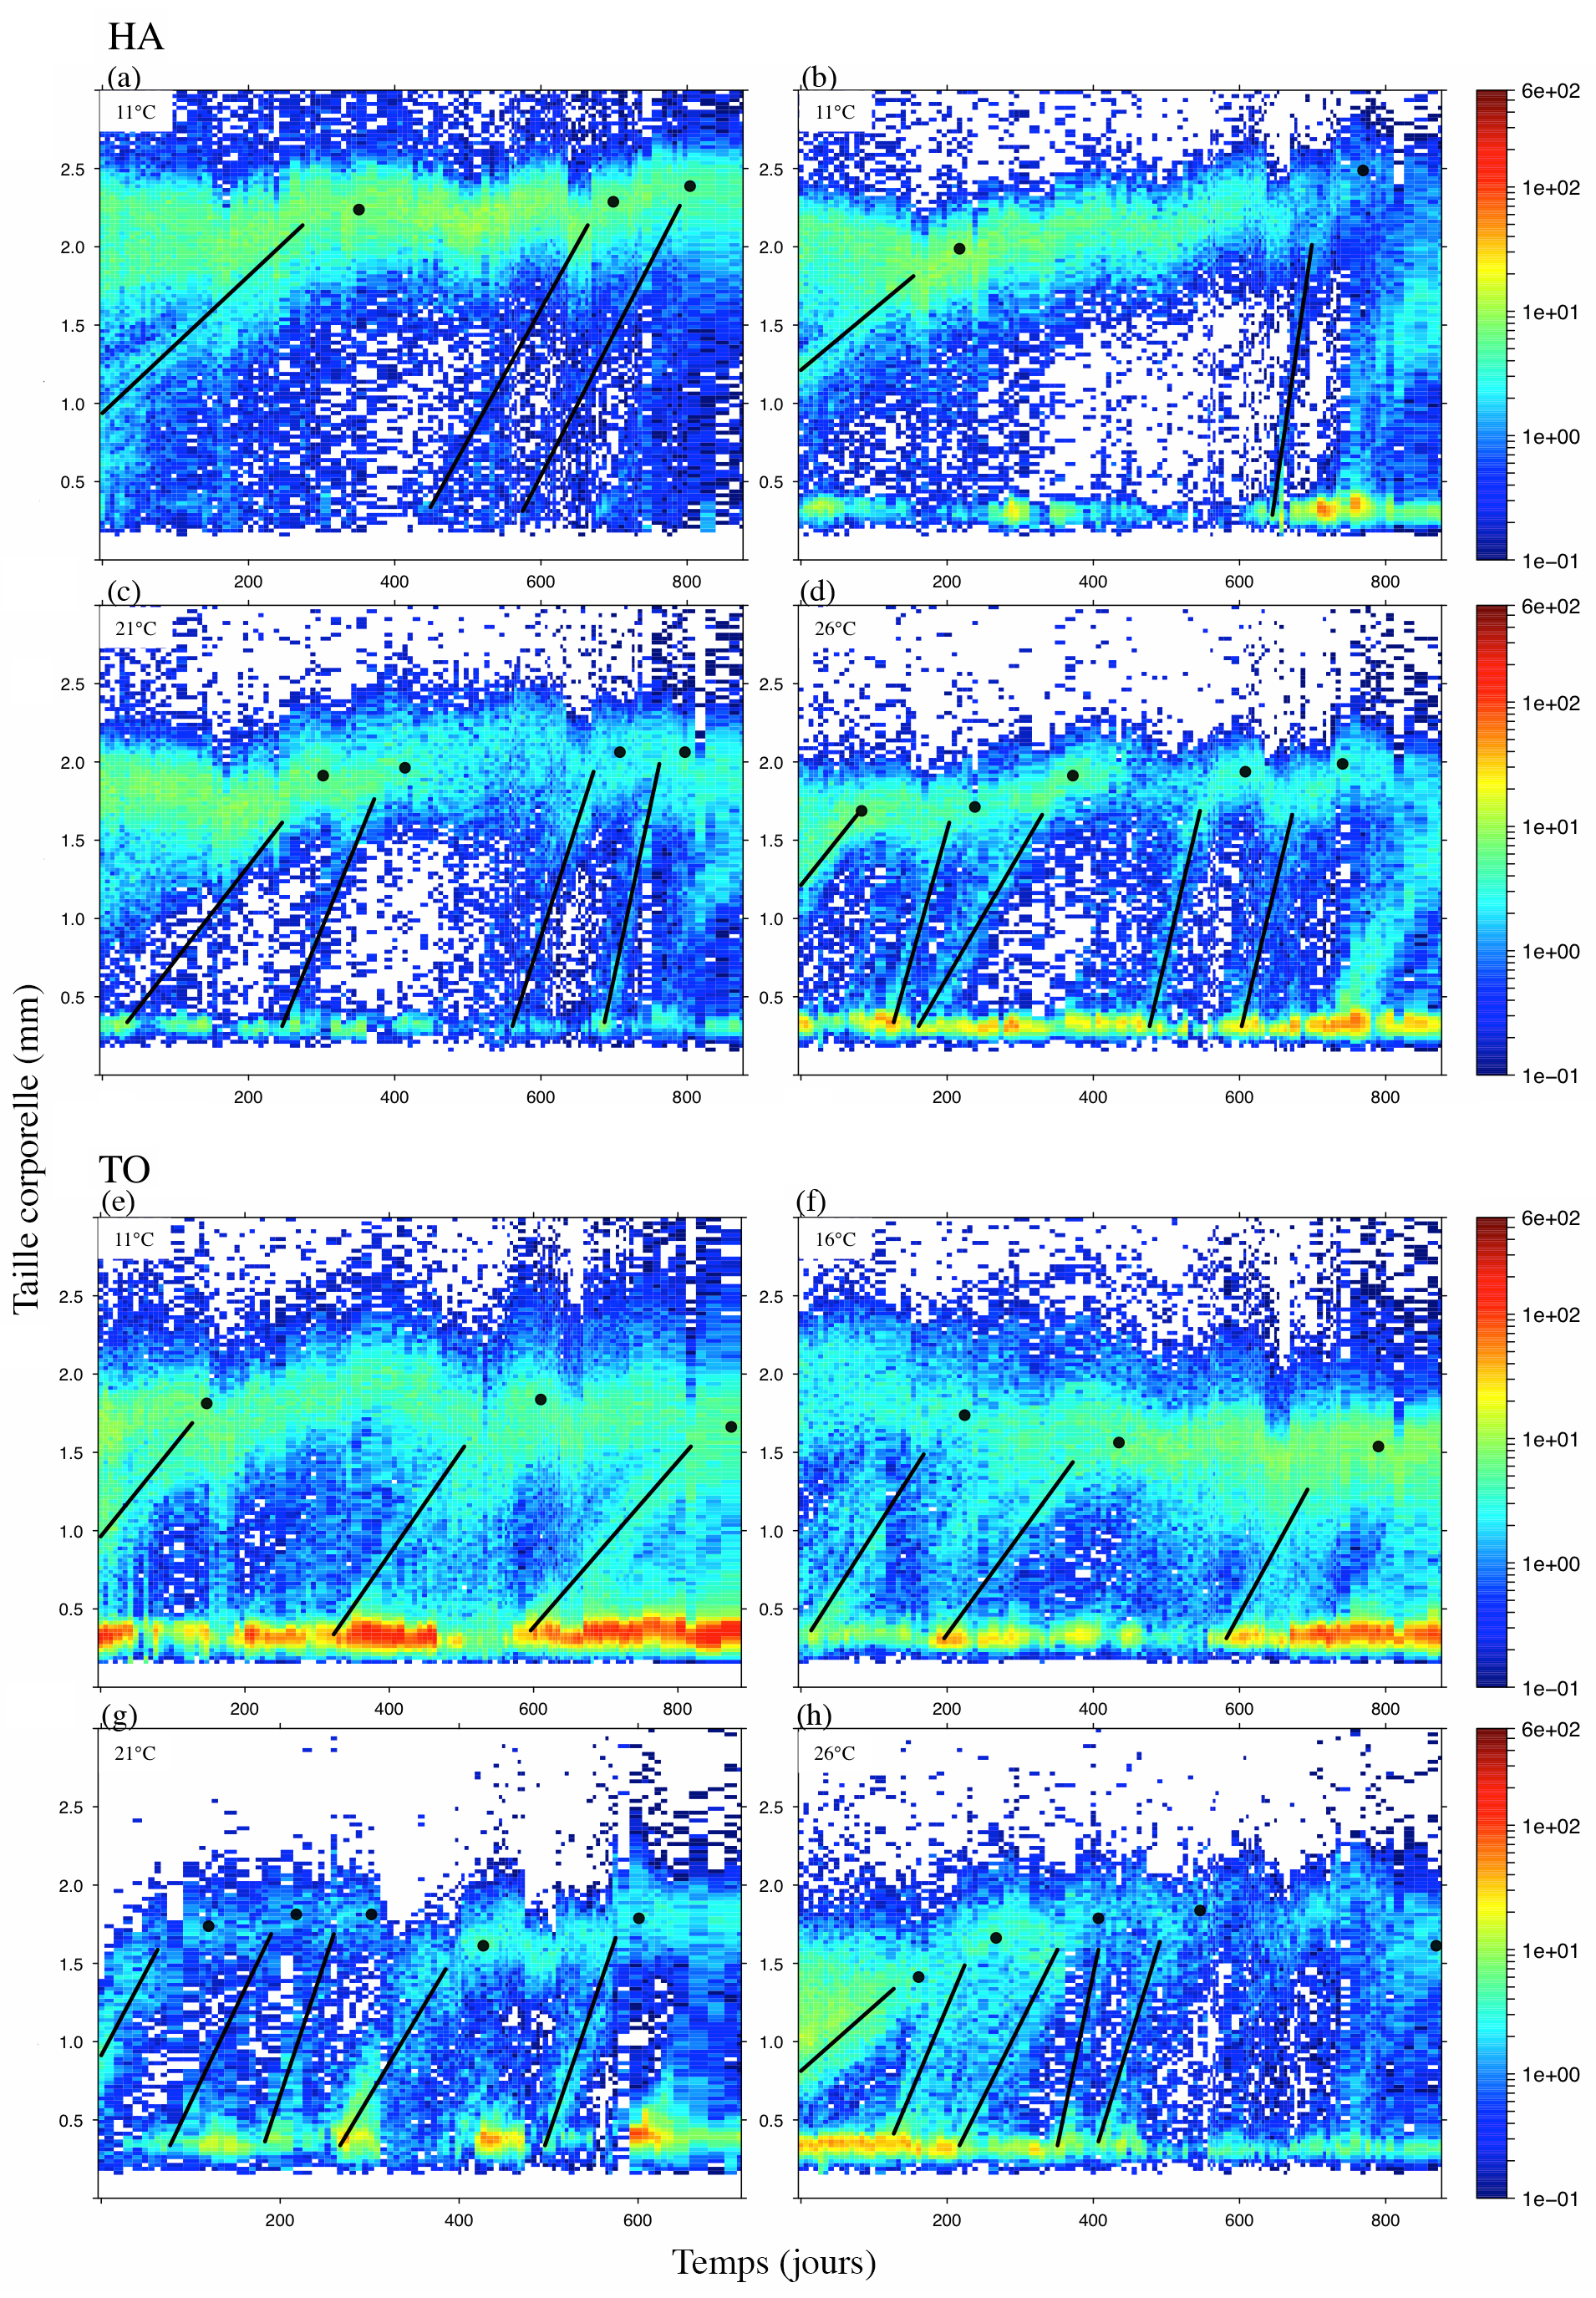
\includegraphics[width=\textwidth]{1_CorpsDeThese/Resumes/Fig/FIP02}
\caption[\lofimage{1_CorpsDeThese/Resumes/Fig/FIP02}Exemples de diagrammes
structures temps]{Exemples de diagrammes
structures temps pour les clones HA
(a-d) et TO (e-h) à $11$ (a et e), 16 (b et f), 21 (c et g) et $26\degres$C
(d et h). Les points noirs marquent les mesures de taille
adulte, tandis que les lignes marquent les mesures de
croissance de cohortes.}
\label{fig:FIP2}
\end{center}
\end{figure}

De la même façon, nous avons étudié la taille des adultes dans les populations
en la comparant aux mesures effectuées sur les individus isolés. Plus
précisément, nous avons construit un indicateur que nous appelons
``\textbf{l'effort de croissance au-delà de la maturité}'' ($GEBM$: ``Growth
Effort Beyond Maturation''). Cet indicateur représente l'investissement dans la
croissance après avoir atteint la maturité dans les populations comparé
à l'investissement en isolation. Il dépend de la température et se calculs comme
la proportion de croissance au-delà de la taille à maturité (mesurée en
isolation) comparée à la taille maximale mesurée en isolation:

\begin{equation}
GEBM(T) = \frac{Taille\ adulte_{populations}(T) -
Taille\ \grave{a} \ maturit\acute{e}_{isolation}(T)}{Taille\ adulte_{isolation}(T) -
Taille\ \grave{a} \ maturit\acute{e}_{isolation}(T)}
\end{equation}

A une température donnée, la taille à maturation et la taille maximale étant
connue pour les individus élevés en isolation, le $GEBM$ nous indique à quel
point un individu continue de croître après la maturation: $GEBM=0$ signifie que
les adultes stoppent leur croissance après la maturation, $GEBM=50\%$ qu'ils
atteignent une taille à mi-chemin de la taille asymptotique en isolation. Des
valeurs inférieures à 0 ou supérieures à $100\%$ signifie respectivement que les
adultes grandissent moins que la taille moyenne à maturité en isolation, ou
qu'ils grandissent plus que la taille maximale moyenne en isolation. N'ayant pas
trouvé de différence significative entre les deux clones, toutes les valeurs de
$GEBM$ ont été regroupées pour les analyses. Nous avons construit des modèles
linéaires avec comme variables explicatives la densité d'adultes, la
température et la lignée clonale avec toutes les interactions possibles. La
significativité des effets a été mesurées à l'aide d'ANOVA et de tests de
Fisher.

\section{Résultats}

\subsection{Norme de réactions à la température}

\subsubsection{Taux de croissance}

\begin{figure}[!ht]
\begin{center}
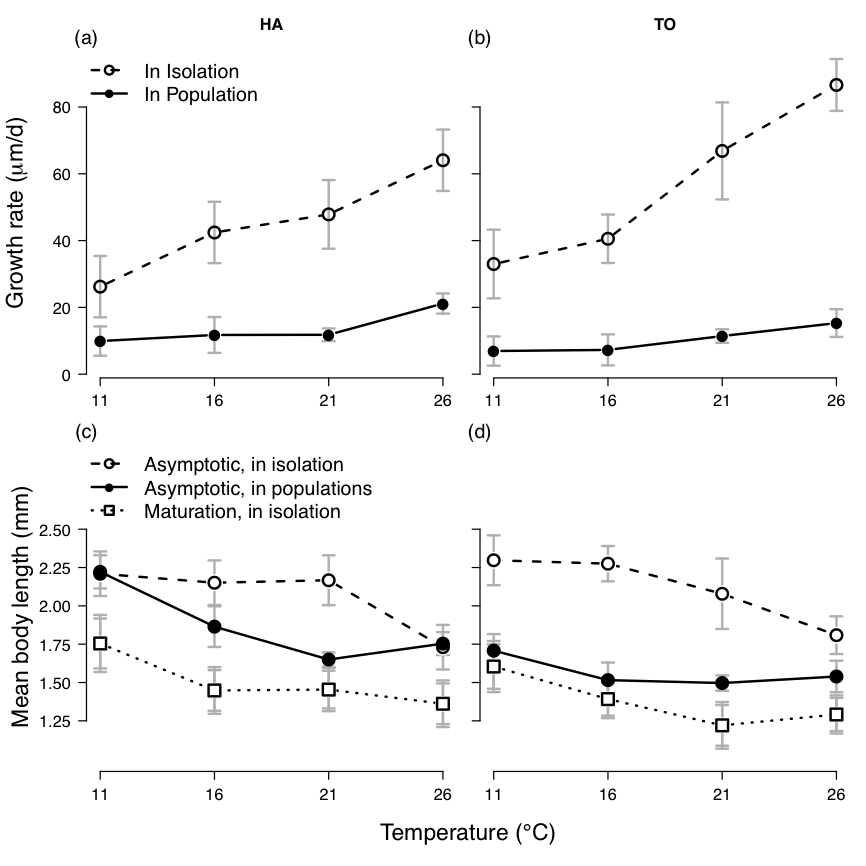
\includegraphics[width=0.95\textwidth]{1_CorpsDeThese/Resumes/Fig/FIP03}
\caption[\lofimage{1_CorpsDeThese/Resumes/Fig/FIP03}Normes de réactions des taux
de croissance et tailles moyennes]{Normes de réactions des taux de croissance (a
et b, moyennes et intervalles de confiance à $95\%$) pour les clones HA (a) et TO (b) mesurés en isolation (tirets) et sur les cohortes en condition de population (lignes pleines). Normes
de réaction de la taille corporelle (c et d): taille moyenne à maturité
(pointillés) et taille asymptotique des individus isolés (tirets) comparés à la
taille adulte moyenne en populations (lignes pleines).}
\label{fig:FIP3}
\end{center}
\end{figure}

La Figure \ref{fig:FIP3} représente les taux de croissance et les différentes
tailles mesurées en isolation ou en populations pour les deux clones. On peut
observer qu'en isolation, le taux de croissance individuel augmente quasiment
linéairement avec la température chez les deux clones (Figure \ref{fig:FIP3}a
et b). A $11\degres$C, les taux de croissance ne sont pas différents entre HA et
TO. Mais le taux de croissance augmente plus vite avec
la température chez TO que chez HA. Il en résulte à
$26\degres$C un taux de croissance $25\%$ supérieur chez TO par rapport à HA. 

Dans les populations, les taux de croissance mesurés sont beaucoup plus faibles
qu'en isolation (Figure \ref{fig:FIP3}a et b). En moyenne, il semble que les
juvéniles du clone HA grandissent plus vite que ceux de TO, mais l'effet de la
température sur les taux de croissance est le même pour les deux clones. 

\subsubsection{Tailles à maturité et taille asymptotique}

Chez les deux clones, les individus isolés suivent quasiment les mêmes normes de
réaction à la température, que ce soit pour la taille asymptotique ou pour la
taille à maturité (Figure \ref{fig:FIP3}c et d). Comme prédit par la règle
taille-température, la taille asymptotique diminue avec la température pour les
deux clones, sans différence significative entre eux. De plus, à part à
$11\degres$C où HA mature légèrement plus grand que TO, la taille à maturité
diminue avec la température de façon similaire pour les deux clones. 

Contrairement aux individus isolés, l'effet de la température sur la taille
moyenne des adultes en condition de population est différent pour les deux
clones. A $11\degres$C, les cohortes du clone HA atteignent en population une
taille qui n'est pas significativement différente de la taille asymptotique en
isolation (Figure \ref{fig:FIP3}c). Puis cette taille adulte moyenne décroît
progressivement pour être proche de la taille à maturité à une température de $21\degres$C. Mais de façon
beaucoup plus étonnante, la taille moyenne des adultes dans les populations du
clone HA ré-augmente entre 21 et $26\degres$C. 

Chez le clone TO à $11$ et $16\degres$C, les cohortes dans les populations
s'arrêtent de grandir peu de temps après avoir atteint leur taille à maturité
attendue d'après les mesures en isolations. Entre $16$ et $26\degres$C, la
taille moyenne des adultes reste statistiquement constante à une valeur intermédiaire
entre la taille à maturité et la taille asymptotique, toutes deux mesurées en
isolation (Figure \ref{fig:FIP3}d).

\subsection{Densité dépendance et température}

\begin{table}[!b]
\centering
\caption{\label{tab:FIP1}Résultats du modèle pour le taux de croissance relatif
des cohortes de juvéniles dans les populations.}
\scriptsize
\begin{tabular}{rccccl}
\hline 
\multicolumn{6}{c}{$lm(\text{taux de croissance} \sim (\log(\text{Densité
d'adultes}) + \text{Température}) * \text{Clone})$} \\
&&&&&\\
& Estimation & Erreur standard & Valeur $t$ & $\text{Pr}(>|t|)$ & \\
\hline

Intercepte = Clone HA, Température 11 & $1.22e+00$ & $8.59e-02$ & $1.42e+01$
& $<2e-16$ & $***$\\

$\log(\text{Densité d'adultes})$ & $-1.48e-01$ & $1.34e-02$ & $-1.10e+01$ & $<
2e-16$ & $***$\\

$\text{Température}$ & $-1.57e-02$ & $1.82e-03$ & $-8.60e+00$ & $8.61e-15$ & $***$\\

$\text{CloneTO}$ & $-4.90e-01$ & $1.18e-01$ & $-4.15e+00$ & $5.56e-05$ & $***$\\

$\log(\text{Densité d'adultes}):\text{CloneTO}$ & $6.79e-02$ & $1.86e-02$ & $3.65e+00$ &
$3.61e-04$ & $***$\\

$\text{Température}:\text{CloneTO}$ & $5.24e-03$ & $2.63e-03$ & $2.00e+00$ &
$4.79e-02$ & $*$\\

\hline 
\end{tabular} 
\end{table}

Pour comprendre les différences entre les normes de réaction mesurées sur les
individus isolés et sur les cohortes en populations, nous avons étudié la
réponse à la température et à la densité de nos deux indicateurs, le taux de
croissance relatif et le $GEBM$, et ce pour les deux lignées clonales. Nous
avons utilisé la densité d'adultes dans les populations comme mesure de densité
car les adultes représentent en moyenne $90\%$ de la biosurface totale des
populations, et nous avons pu démontrer leur rôle prépondérant dans la dynamique
des populations structurées (voir Chapitres \ref{chap:sp} à \ref{chap:sm} et
Annexes \ref{Ann:SP} et \ref{An:AmNat}).

\subsubsection{Taux de croissance relatif}

\begin{figure}[!ht]
\begin{center}
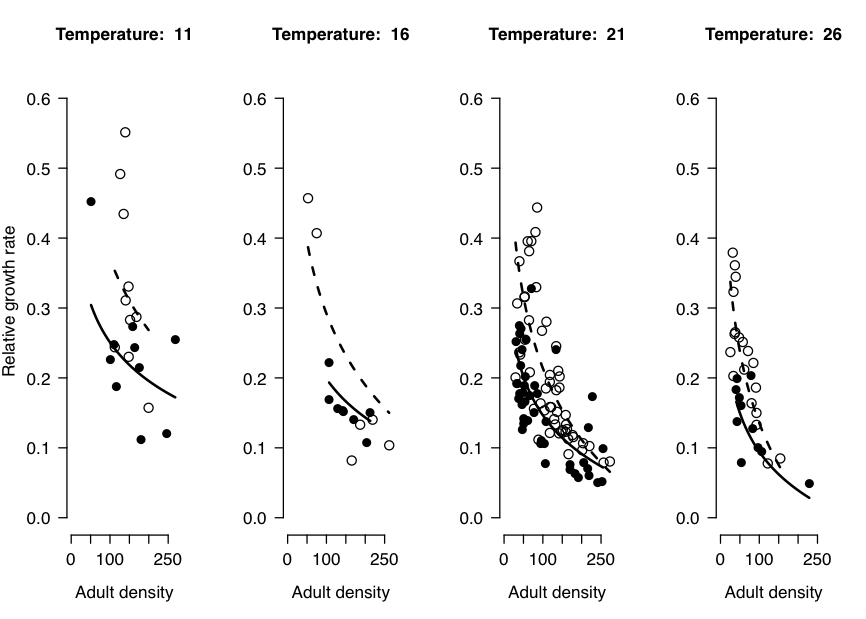
\includegraphics[width=\textwidth]{1_CorpsDeThese/Resumes/Fig/FIP04}
\caption[\lofimage{1_CorpsDeThese/Resumes/Fig/FIP04}Taux de croissance
relatifs]{Taux de croissance relatifs en fonction de la densité d'adultes dans
les populations pour les clones HA (lignes tiretées et symboles ouverts) et TO
(lignes pleines et symboles pleins)}
\label{fig:FIP4}
\end{center}
\end{figure}

A chaque température, le taux de croissance des cohortes de juvéniles dans les
populations diminue avec la densité d'adultes en suivant une loi exponentielle
(Figure \ref{fig:FIP4}, Table \ref{tab:FIP1}). En moyenne, les juvéniles des
populations du clone HA grandissent plus vite que ceux du clone TO, mais l'effet
délétère de la densité d'adulte y est également plus fort. Les différences
génétiques entre les clones ont donc tendance à s'atténuer avec la densité. 

L'augmentation de la température a également tendance à réduire le taux de
croissance relatif des cohortes. Cet effet est légèrement plus intense pour HA,
mais cela est probablement dû à un taux de croissance plus élevé que TO à
faible densité. 

\subsubsection{Effort de croissance après maturation}

\begin{figure}[!ht]
\begin{center}
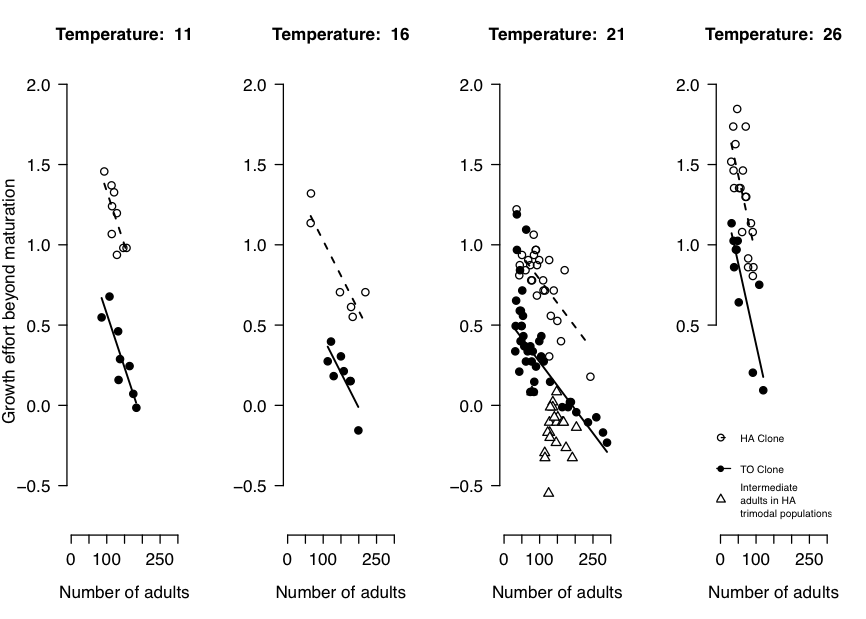
\includegraphics[width=\textwidth]{1_CorpsDeThese/Resumes/Fig/FIP05}
\caption[\lofimage{1_CorpsDeThese/Resumes/Fig/FIP05}GEBM]{Effort de croissance
après maturité ($GEBM$) en fonction de la densité d'adultes pour les quatre
températures. }
\label{fig:FIP5}
\end{center}
\end{figure}

La plupart des populations étudiées possèdent une structure bimodale similaire à
celles décrites dans le Chapitre \ref{chap:sp} (voir aussi Annexe \ref{Ann:SP}).
Cela permet de discriminer les adultes des juvéniles (voir Supplementary Materials de l'Annexe \ref{Ann:fip})
et ainsi d'estimer la densité et la taille moyenne des adultes afin d'estimer le
$GEBM$. La Figure \ref{fig:FIP5} montre que les réponses du $GEBM$ à la
densité et à la température diffèrent quantitativement mais pas qualitativement
entre les deux lignées (voir aussi Table \ref{tab:FIP2}). En moyenne, le $GEBM$
de HA est supérieur à celui de TO, indépendamment de la température. Cependant,
les différences entre clones s'atténuent avec la température. Pour chaque clone,
le $GEBM$ est négativement corrélé à la densité d'adultes: plus la densité
d'adultes est grande, plus leur taille moyenne se rapproche de la taille à
maturité mesurée sur les individus isolés à la même température. La pente de
cette corrélation et la même pour les deux clones à chaque température et donne
une mesure de la dépendance à la densité. 

\begin{table}
\centering
\caption{\label{tab:FIP2}Résultats du modèle pour le taux de croissance relatif
des cohortes de juvéniles dans les populations.}
\scriptsize
\begin{tabular}{rccccl}
\hline 
\multicolumn{6}{c}{$lm(GEBM \sim (\text{Densité
d'adultes} + \text{Clone}) * \text{Température})$} \\
&&&&&\\
& Estimation & Erreur standard & Valeur $t$ & $\text{Pr}(>|t|)$ & \\
\hline

Intercepte = Clone HA, Temperature11 & $2,01E+00$ & $1,93E-01$ & $1,04E+01$ & $<
2e-16$ & $*** $\\
Température16 & $-5,43E-01$ & $2,43E-01$ & $-2,23E+00$ & $2,77E-02$ & $* $\\
Température21 & $-9,25E-01$ & $1,98E-01$ & $-4,68E+00$ & $8,18E-06$ & $*** $\\
Température26 & $-7,06E-02$ & $2,10E-01$ & $-3,37E-01$ & $7,37E-01$ & $ $\\
Densité d'adultes & $-6,72E-03$ & $1,50E-03$ & $-4,48E+00$ & $1,84E-05$ & $*** $\\
CloneTO & $-7,62E-01$ & $7,88E-02$ & $-9,68E+00$ & $< 2e-16$ & $*** $\\
Densité d'adultes:Temperature16 & $2,35E-03$ & $1,77E-03$ & $1,33E+00$ & $1,87E-01$ & $ $\\
Densité d'adultes:Temperature21 & $3,76E-03$ & $1,53E-03$ & $2,46E+00$ & $1,56E-02$ & $* $\\
Densité d'adultes:Temperature26 & $-3,34E-03$ & $1,91E-03$ & $-1,75E+00$ & $8,36E-02$ & $. $\\
Température16:CloneTO & $1,58E-01$ & $1,15E-01$ & $1,37E+00$ & $1,73E-01$ & $
$\\
Température21:CloneTO & $2,48E-01$ & $8,80E-02$ & $2,82E+00$ & $5,71E-03$ & $**
$\\
Température26:CloneTO & $2,13E-01$ & $9,93E-02$ & $2,15E+00$ & $3,39E-02$ & $*
$\\

\hline 
\end{tabular} 
\end{table}

Comme observé au cours du Chapitre \ref{chap:sp} (voir aussi Annexe
\ref{Ann:SP}), certaines populations du clone HA à $21\degres$C exhibent une structure trimodale avec deux groupes d'adultes
stabilisés à des tailles différentes. Nous pouvons dès lors calculer le $GEBM$
indépendamment pour les deux groupes d'adultes.
Dans ces populations, nous avons trouvé un $GEBM$ très différents pour les deux
groupes d'adultes (Figure \ref{fig:FIP6}). Alors que les adultes les plus grands
ont un $GEBM$ qui suit le même modèle général que pour les autres populations,
le $GEBM$ des adultes les plus petits n'est pas expliqué par le nombre total
d'adultes dans les populations. Nous n'avons pas non plus trouvé de corrélation
significative entre le nombre d'adultes de petite taille et leur $GEBM$. En
revanche, à la fois le nombre d'adultes de petite taille et leur taille moyenne
sont corrélés au nombre d'adultes de plus grande taille. Nous avons donc
modélisé le $GEBM$ de tous les groupes d'adultes du clone HA à $21\degres$C à
l'aide du nombre d'adultes de plus grande taille (ou du nombre total d'adultes
pour les structures bimodales). Il est intéressant de constater qu'il n'y a
alors pas de différence significative dans la pente de la régression entre le
$GEBM$ des adultes de grande taille et celui des plus petits, seulement dans
leur intercepte (Figure \ref{fig:FIP6}). Dans les populations trimodales, la
présence d'adultes de grande taille agit donc sur le $GEBM$ des plus petits de
la même façon que si les populations étaient bimodales avec des petits adultes,
mais en densité supérieure ($260$ adultes de plus, voir Figure \ref{fig:FIP6}).

\begin{figure}[!ht]
\begin{center}
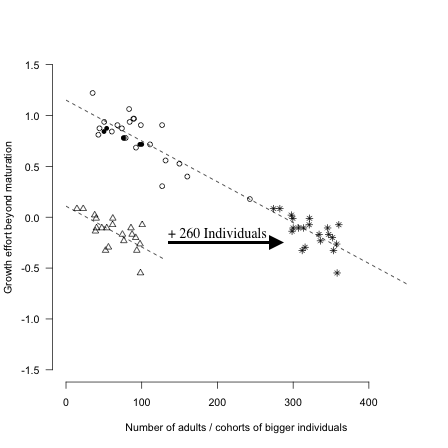
\includegraphics[width=0.75\textwidth]{1_CorpsDeThese/Resumes/Fig/FIP06}
\caption[\lofimage{1_CorpsDeThese/Resumes/Fig/FIP06}GEBM dans les
populations HA à $21\degres$C]{GEBM dans les
populations HA à $21\degres$C pour les adultes de petite taille ($\triangle$) et
de grande taille ($\circ$) dans les populations trimodales, et pour les petits
adultes s'il y avait 260 petits adultes de plus à la place des grands ($\ast$).}
\label{fig:FIP6}
\end{center}
\end{figure}

\subsubsection{Normes de réaction à la température des indicateurs}

L'indicateur $GEBM$ dépend également de la température pour nos deux lignées
clonales. Cependant, contrairement au taux de croissance relatif, l'effet de la
température sur $GEBM$ n'est pas linéaire. Afin d'étudier l'effet de la
température sur nos deux indicateurs en contrôlant pour l'effet de la densité au
sein de chacun des clones, nous avons tracé les taux de croissance relatifs et
$GEBM$ prédits pour une densité de 100 adultes en utilisant les modèles ajustés
pour chaque lignée indépendamment (Figure \ref{fig:FIP7a}). 

\begin{figure}[!ht]
\begin{center}
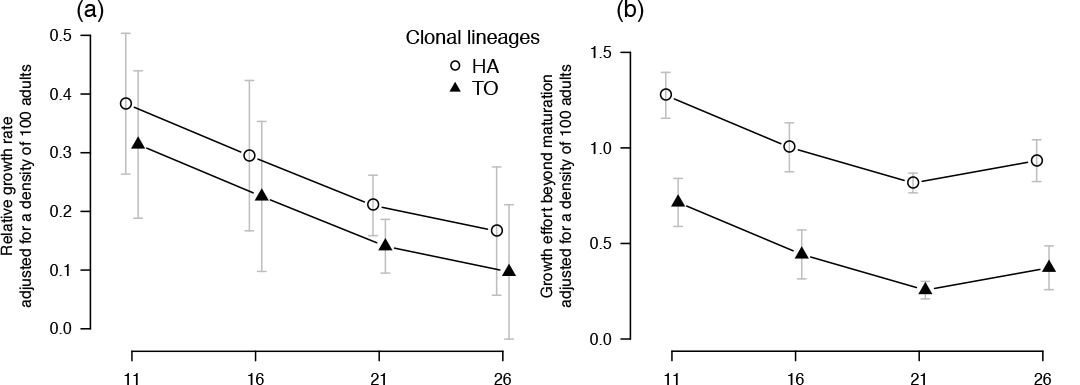
\includegraphics[width=0.75\textwidth]{1_CorpsDeThese/Resumes/Fig/FIP07a}
\caption[\lofimage{1_CorpsDeThese/Resumes/Fig/FIP07a}Normes de réaction
prédites à la température]{Normes de réaction à la température prédites pour
une densité de 100 adultes. (a) Taux de croissance relatif. (b) Effort de
croissance après maturation.}
\label{fig:FIP7a}
\end{center}
\end{figure}

Dans les deux lignées génétiques, le taux de croissance relatif décroît
linéairement avec la température (Figure \ref{fig:FIP7a}a), mais la norme de
réaction de $GEBM$ suit une forme en U: $GEBM$ décroît entre $11$ et
$21\degres$C mais augmente ensuite jusqu'à $26\degres$C (Figure
\ref{fig:FIP7a}b). Cette augmentation de $GEBM$ à la température la plus chaude
testée est remarquable car dans la plupart des populations élevées à $26\degres$C, la
taille adulte moyenne est plus grande que la taille asymptotique mesurée sur les
individus isolés à la même température (Figure \ref{fig:FIP5} à $21$ et
$26\degres$C), alors qu'à $21\degres$C chez HA, certaines cohortes n'atteignent
pas la taille à maturité mesurée en isolation (Figure \ref{fig:FIP5} à
$21\degres$C, valeurs négatives).

\section{Discussion}

\subsection{Normes de réaction des individus isolés}

Les normes de réactions mesurées sur des individus isolés montrent que les
Collemboles de l'espèce \textit{Folsomia candida} suivent la règle dite
``taille-température'' \autocites{atkinson1994a,angilletta2009a}. En effet,
dans des conditions froides, les individus grandissent plus lentement mais
atteignent des tailles supérieures à des individus isolés élevés dans des
conditions plus chaudes \autocites{angilletta2003a}. Bien que des études aient
déjà montré des effets similaires de la température sur les taux de croissance
de collemboles juvéniles \autocites{birkemoe2000a, driessen2007a, ellers2008a,
ellers2011b} ou sur la taille à maturité \autocites{stam1996a}, cette étude est
à notre connaissance la première à démontrer expérimentalement un ajustement
plastique de la taille adulte à différentes conditions de température ambiante.
Malgré des stratégies démographiques différentes entre les deux clones étudiés
\autocites{tully2008a,tully2011a}, les différences génétiques entre les clones
n'entraînent que très peu de différence dans les normes de réaction
individuelles à la température de la taille adulte, ce qui est similaire à ce
qui a déjà été observé chez un autre Collembole \autocites{driessen2007a}.

\subsection{Densité dépendance dans les populations}

Cette étude expérimentale constitue à notre connaissance la première description
expérimentale quantitative de dynamiques de populations structurées en taille le
long d'un gradient de température relativement large. Ces populations ont
généralement une structure bimodale avec un mode d'adultes et un mode de
juvéniles distincts. La plupart du temps, les juvéniles ne montrent pas de
croissance visible, mais un groupe de juvéniles parvient périodiquement à
grandir et recruter chez les adultes 

Que ce soit pour les taux de croissance ou les taille adultes, les normes de
réactions à la température en conditions de population sont différentes de
celles mesurées sur les individus isolés, avec des valeurs en moyenne plus
basses en population, probablement à cause de la compétition à l'\oe{}uvre pour
l'accès aux ressources (voir les Chapitres précédents). Dans nos populations,
l'apport de ressource est le même quel que soit la température ambiante. Les
populations atteignent donc un équilibre dynamique où la quantité de ressource
disponible limite le nombre, la taille corporelle et l'investissement
reproductif des adultes. Les équilibres atteints par les populations résultent
de rétroactions complèxes entre des stratégies démographiques
\autocites[dépendantes des clones,][]{tully2008a,stam1996a} et les effets de la
densité dépendance \autocites{kokko2007a} qui proviennent principalement de deux
mécanismes: la compétition pour la nourriture et pour l'espace. 

Comme montré dans les Chapitres précédents, la compétition pour la nourriture
est un des facteurs principaux de régulation de la dynamique de
nos populations de Collemboles. Cette compétition régule également les taux de
croissance des cohortes de juvéniles et les tailles corporelles atteintes par
les adultes (voir Chapitres \ref{chap:sp}, \ref{chap:amnat}, \ref{chap:sm} et
Annexes \ref{Ann:SP} et \ref{An:AmNat}).
Les effets négatifs de la densité sont visibles à deux échelles: (i) en
comparant les traits mesurés en populations aux traits mesurés sur des individus
isolés; et (ii) en comparant les traits mesurés dans des populations avec
différentes densités d'adultes. Nous avons montré dans cette étude que l'effet
négatif de la densité sur les traits d'histoire de vie peut être très fort (les
taux de croissance en population n'atteignent par exemple que 20 à $30\%$ des
valeurs mesurées sur des individus isolés). Cet effet de densité prend alors le
pas sur la plupart des ajustements plastiques dont les individus sont capables à
différentes températures. 

La comparaison des deux clones étudiés a permis de mettre en évidence des
différence génétiques significatives dans l'intensité de la densité dépendance:
pour les deux traits étudiés, le clone HA souffre d'avantage d'une augmentation
de la densité d'adultes que le clone TO, et cela à toutes les températures
testées. Ces réponses différentes à la densité pourraient provenir de
différences génétiques dans la sensibilité des juvéniles à la densité d'adultes
ou dans le niveau de compétition que les adultes imposent aux juvéniles. Afin de
discriminer entre ces deux hypothèses, on pourrait envisager une expérience où
l'on mesurerait les taux de croissance et les tailles atteintes par les juvéniles
de chaque clone élevés en présence d'adultes des deux clones. 

\subsection{Normes de réaction en population}

Le long du gradient de température testé, nous avons constaté que la plasticité
phénotypique observable chez les individus isolés est annulée voir inversée en
condition de population. Les interactions compétitives que les individus
subissent dans les populations suffisent à réduire fortement les taux de
croissance des juvéniles qui sont alors quasiment constants aux différentes
températures. Cependant, en comparant ces taux de croissance à ceux des
individus isolés et en contrôlant pour la densité, nous avons pu montrer un
effet négatif de la température: l'effet négatif de la densité sur les taux de
croissance est donc amplifié lorsqu'on augmente la température. Cela suggère que
l'intensité de la compétition subie par les juvéniles dans nos populations
augmente avec la température, ce qui est cohérent avec l'augmentation des taux
physiologiques à haute température \autocites{gillooly2001a}.

La taille moyenne des adultes dans les populations est elle aussi négativement
corrélée à la densité. Entre 11 et $21\degres$C, la diminution du $GEBM$ avec la
température montre que la taille moyenne des adultes dans les populations tend à
se rapprocher de la taille à maturité mesurée sur les individus isolés. De plus,
l'augmentation de la température provoque l'augmentation des taux de
consommation de la ressource alors même que l'apport de nourriture reste
constant. Des résultats théoriques ont montré que dans ces conditions,
l'augmentation de la température amplifie l'avantage compétitif des plus jeunes
lié à leur plus grande efficacité dans la gestion de l'énergie
\autocites{ohlberger2011a}.
De plus, d'après les modèles de populations physiologiquement structurées, cet
avantage compétitif dans le cas de l'exploitation fait converger la taille
maximale atteinte par les adultes vers la taille à maturité. Ainsi, la
diminution du $GEBM$ entre 11 et $21\degres$C pourrait être due à une
augmentation avec la température de l'intensité de la compétition par
exploitation. 

Cependant, au-delà de $21\degres$C, on observe la tendance inverse avec une
augmentation du $GEBM$. Cela ne peut pas être expliqué par une plus faible
densité, ni par un effet direct de la température sur les individus.
Ceci laisse donc entendre que l'augmentation de la compétition par exploitation
avec la température n'est pas le seul phénomène responsable des effets de la densité
dépendance dans nos populations. Alors que l'augmentation de la compétition par
exploitation fait tendres les tailles adultes vers la taille à maturité,
une augmentation de la compétition par interférence provoque l'émergence
d'individus de très grande taille (voir Chapitre \ref{chap:amnat} et Annexe
\ref{An:AmNat}).
L'importance relative des deux types de compétition pourrait donc être à l'origine de la
réponse plastique de la taille adulte dans les populations. Alors que la
compétition par exploitation est probablement dominante à faible température du
fait de l'activité réduite des individus, si la compétition par interférence
augmente plus rapidement avec la température que la compétition par
exploitation, elle pourrait finir par dominer à partir d'une certaine
température et favoriser les grands individus malgré une
température élevée, tel que proposé sur la Figure \ref{fig:FIP7b}.

\begin{figure}[!ht]
\begin{center}
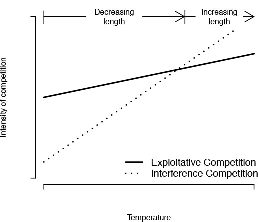
\includegraphics[width=0.5\textwidth]{1_CorpsDeThese/Resumes/Fig/FIP07b}
\caption[\lofimage{1_CorpsDeThese/Resumes/Fig/FIP07b}Importance relative
des différentes formes de compétitions]{Importance relative
des différentes formes de compétitions avec la température et leurs effets sur
la taille des adultes en condition de population.}
\label{fig:FIP7b}
\end{center}
\end{figure}

Les résultats présentés sur les populations HA trimodales montrent également que
la cohorte d'individus les plus grands imposent la densité et la taille de la
cohorte d'adultes plus petits. Ceci démontre encore une fois le rôle de la
compétition par interférence dans la régulation de nos populations, où un
adulte de grande taille reproduits les effets de densité dépendance produits par
quatre adultes de petite taille. La taille des plus grands adultes étant environ
deux fois supérieure à celle des adultes les plus petits dans les populations
trimodales, ce facteur d'environ 4 apporte par ailleurs un argument venant
appuyer l'hypothèse de la densité ressentie par les individus dépendante de la
longueur au carré dans le modèle présenté dans le Chapitre \ref{chap:amnat}, eq.
\refeq{eq_an2} page \pageref{eq_an2} (voir aussi Annexe \ref{An:AmNat}): $$
\eta(t,l)=\int_{l_b}^{l_m} \! C(l,\lambda)\cdot n(t,\lambda)\cdot\lambda^2\, \mathrm{d}\lambda $$.

Les mécanismes par les quels la température agit sur la compétition par
interférence ne sont cependant pas clairs. Nous avons montré dans le Chapitre
\ref{chap:sm} que les individus les plus grands empêchaient les plus petits
d'accéder à la ressource. Nous pensons que l'augmentation de la température, en
augmentant les taux métaboliques et l'activité augmentent à la fois la fréquence
à la quelle les collemboles sont en besoin de nourriture (2 fois par cycle de
vie, \citealp{palevody1974a}) alors que l'apport reste constant, et la fréquence
des interaction directes entre les individus, augmentant de ce fait l'intensité
de la compétition par interférence. 

La forme en U des normes de réactions de $GEBM$ pourrait donc être dues à
l'augmentation simultanée de la compétition par exploitation et par
interférence, mais avec des vitesses différentes (Figure \ref{fig:FIP7b}). En
dessous d'une température critique, bien qu'augmentant moins vite, la
compétition par exploitation reste la force régulatrice majeure de la dynamique
des populations, et l'augmentation de la température provoque alors une
diminution de la taille adulte qui tend vers la taille à maturité. Au-delà de la
température critique, la compétition par interférence devient dominante, et
l'augmentation de la température, en augmentant l'intensité de l'interférence,
favorise finalement des individus de grande taille. Dans ce cadre, l'existence
de populations trimodales à $21\degres$C, décrites dans les Chapitre précédents,
pourrait également être expliquée par des compétitions par exploitation et par
interférence relativement équilibrées qui ainsi permettrait l'émergence de
grands individus mais ne permettrait pas l'arrêt complet de la croissance des
juvéniles qui pourraient quand même maturer et s'arrêter de grandir à une taille
adulte intermédiaire. Ceci constitue donc une hypothèse complémentaire à
celle des conditions initiales pour l'apparition de ces populations trimodales.
En effet, bien qu'aillant des conditions initiales identiques, seules certaines
populations à $21\degres$C ont atteint des structures trimodales, jamais aux
autres températures. 

\section{En conclusion}

En mesurant des traits d'histoire de vie à la fois sur des individus isolés et
dans des populations, nous avons pu montrer que: (i) les effets de la densité
dépendance peuvent l'emporter sur les effets de la température attendus d'après
les mesures sur les individus isolés; et (ii) les effets de la densité
dépendance subissent eux-mêmes des changements liés aux conditions de
température. Ceci montre l'importance d'identifier clairement les différentes
composantes de la densité dépendance (compétition par exploitation ou
interférence par exemple) et leurs réponses à la température afin d'être capable
de prédire les réactions des populations aux changements de température en cours
et à venir. 







\partimage[width=\textwidth]{FigParts/writing3}
\part{Conclusion Générale}

\chapter{Dans une coque de noix}
\chaptermark{Dans une coque de noix}

\section{Principaux résultats de la thèse}

Au cours de cette thèse, nous avons exploré certains détails de la dynamique des
populations structurées, à la fois d'un point de vue expérimental que théorique.
Nous avons porté une attention toute particulière aux rôles que jouent les
interactions taille dépendantes entre individus dans l'établissement de ces
dynamiques, d'abord en observant des populations expérimentales de Collembole
\textit{Folsomia candida} sur le long terme pour en analyser les dynamiques en
fonction de leur structure en taille, puis en modélisant les interactions
tailles dépendantes entre individus dans un modèle physiologiquement structuré,
et enfin en manipulant la structure de la population et en observant les
comportement d'accès aux ressources. Nous nous sommes ensuite intéressé à
l'effet de l'environnement, via la température ambiante, sur ces interactions et
les répercussions sur la dynamique des populations.

Dans ce dernier chapitre, nous reviendrons sur les principaux enseignements que
l'on peut tirer de ces travaux par ses développements tant méthodologiques que
théoriques ou expérimentaux.

\subsection{Les développements méthodologiques}

J'ai choisi de revenir ici sur quelques développements méthodologiques réalisés
au cours de cette thèse car ils n'ont pas seulement occupé une grande partie de
mon travail, mais se sont également révélés indispensable au bon déroulement de
ces travaux. 

\subsubsection{Le phénotypage haut débit}

Le développement de la méthode d'analyse d'image pour le dénombrement et la
mesure de la structure des populations a été un élément clé qui a rendu possible
ce travail. Cette méthode de suivi des populations a été initialisées par
Thomas \textcites{tully2004a} au cours de sa thèse, puis reprise en développée
par François \textcites{mallard2013b} et moi même pendant plusieurs années avant
de faire l'objet d'un chapitre dans un ouvrage du CNRS
\autocites{le-galliard2012a} et d'une publication \autocites{mallard2013a}.

La méthode développé a notamment rendu possible la réplication des expériences
dans une mesure que l'on n'aura pas pu atteindre en dénombrant manuellement les
populations. C'est une méthode fiable qui permet à peu de frais d'accéder à la
structure en taille d'une population (et donc à la densité dans les différentes
classes de taille) en peu de temps et de façon très peu voir pas du tout
intrusive. 

Cette méthode a été développée et appliquée à des populations de collemboles,
mais est susceptible d'être facilement transposée à d'autres systèmes
expérimentaux comme cela a été décrit dans \textcites{mallard2013a}, ce qui lui
donne un grand intérêt pour l'écologie expérimentale et l'étude des traits
d'histoire de vie. 

\subsubsection{Diagrammes structure-temps}

Le travail présenté dans cette thèse n'aurait pas non plus été possible sans le
développement de la représentation graphique en diagrammes structure-temps et
des outils d'analyse graphique associés. En effet, cette technique simple de
représentation des données a permis de rendre cohérentes des données d'une
grande richesse dans les quelles il aurait été facile de se perdre. 

Nous pensons que l'application de cette méthode à des séries temporelles
structurées permettra de mettre en évidence des phénomènes qu'il était jusqu'à
présent difficile de décrire. Cette représentation rempli les critères
d'excellence des représentations graphiques en statistiques décrits par
\textcites{tufte1990a} en condensant une grande quantité d'information sur un
petit espace de représentation, sans déformer les données et en révélant
plusieurs niveaux de détails en une seul fois, des structures fines à la vue
d'ensemble \autocites{tufte2001a}. Avec le développement des méthodes
automatisées telles que celle présentée dans cette thèse \autocites[voir aussi
][]{le-galliard2012a} et la croissance toujours accélérée des bases de données
(``big data''), ce type de méthode devrait à l'avenir se démocratiser, autant en
écologie des populations que dans des domaines plus variés comme en
démographie humaine, en épidémiologie, dans les enquêtes d'opinion, d'usage,
\textit{etc}.

\subsection{Taille corporelle et populations structurées}

Au delà des apports méthodologiques, les travaux présentés dans cette thèse
répondent à des questions fondamentales en écologie des populations quant aux
rôle des interactions entre individus au sein d'une population dans la
régulation de sa structure et de sa dynamique, et à la place qu'occupe la taille
corporelle des individus dans la détermination de ces interactions.

\subsubsection{Taille corporelle et compétition par interférence}

Un premier résultat qui ressort de cet étude est l'importance de la différence
de taille corporelle dans la régulation de la dynamique de la structure en
taille de nos populations expérimentales. Nous avons pu montrer au cours des
différentes expériences menées et suivis de populations que la présence de
classes de tailles différentes en densité différentes avait un impact direct sur
la dynamique que l'on pouvait observer, tant à court terme qu'à long terme. La
présence d'individus de grande taille notamment s'est montré un critère
déterminant dans les dynamiques observées dans les différentes populations. 

En observant plusieurs populations dans les mêmes conditions, nous avons pu
montrer que les différentes structures en taille observées sont en nombre
limité, et peuvent être regroupées en quatre grande catégories. Ces catégories
de structures, que l'on a appelé structures types, se différencies par
l'abondance des juvéniles, la taille des adultes, et leur abondance. Une de ces
catégories est particulièrement remarquable par le fait qu'elle contient trois
modes séparés dans la distribution de la taille (les structures de types 4),
contrairement aux trois autres qui n'en contiennent que deux. Cette structure
type n'a par ailleurs été observée que chez un seul des deux clones étudiés, HA,
et cela quelque soit l'expérience menée. Le point commun entre les quatre
types de structure est la présence d'adultes à une taille corporelle stable
nettement supérieure à la taille à maturité, ce qui est contraire aux
prédictions des modèles de populations structurées régulées par compétition
intra-spécifique par exploitation.

L'observation des dynamiques de court terme dans ces populations a permis de
démontrer que ces adultes de taille relativement élevée jouaient un rôle
déterminant dans les dynamiques de la structure des populations. Leur
disparition progressive ou brutale coïncide de façon quasi systématique avec un
événement de recrutement de juvéniles dans les classes adultes. La perturbation
de la structure des populations dans une seconde expérience a permis de
renforcer le lien de causalité entre la présence des adultes et la croissance ou
non des juvéniles. En effet, retirer l'ensemble des adultes d'une de nos
populations de collemboles provoque un événement massif de recrutement alors que
ne retirer qu'une partie des adultes réduit
grandement le nombre de juvéniles qui parviennent à recruter. Lorsque plusieurs
classes de taille coexistent chez les adultes, le retrait des plus grands, même
moins nombreux, provoque un événement de recrutement plus important que le
retrait des plus petits. Retirer des individus de grande taille permet donc de
rendre la possibilité aux juvéniles de grandir et d'atteindre la maturité.

Cette domination des adultes sur la dynamique de la structure de nos populations
s'explique par la domination qu'ils exercent sur l'accès à la ressource fournie.
Cette hypothèse, issue de l'observation des séries temporelle de la structure
des populations, a été confirmée par l'observation des comportements d'accès à
la ressource et la mesure du biais de taille dans cet accès. Par ces mesures, on
a pu montrer une sur-représentation systématique des individus les plus grands
au contact ou aux abords de la pastille de ressource. Cette pastille de
ressource étant très localisée comparé à l'environnement de vie des Collemboles,
il est alors facile pour la minorité d'individus les plus grands de monopoliser
la ressource et d'en restreindre l'accès aux plus petits. Ces derniers ne
pouvant se nourrir ne peuvent alors pas se développer et restent dans un stade
juvénile jusqu'à ce que le nombre d'adultes diminue suffisamment pour que la
ressource deviennent à nouveau accessible. 

Ce comportement des individus les plus grands repoussant les plus petits aux
abords de la ressource et ses conséquences sur la dynamique de la structure
montrent l'existence d'une compétition par interférence, parfois de forte
intensité, dans nos populations de collemboles. Cette compétition par
interférence contre balance l'avantage énergétique que possèdent les petits
individus et permets ainsi au plus grands de survivre et de dominer la
population. 

\subsubsection{Compétition par interférence et dynamique des populations
structurées}

Nous avons donc montré le rôle de la compétition par interférence dans la
régulation de nos populations structurées en taille, et notamment comment elle
permettait la survie d'individus de grande taille, et parfois de géants très
longévives qui, même en petit nombre, dominent le reste de la population. 

Afin d'étudier plus avant les conséquence de l'existence d'une compétition
intra-spécifique par interférence sur la dynamique d'une population structurée,
nous avons repris le modèle classique de dynamiques de populations
physiologiquement structurées développé pour les Daphnies
\autocites{kooijman1984a}. Nous avons adapté ce modèle à notre système en le
paramétrant pour les collemboles, ce qui a été possible car le cycle de vie des
collemboles présente des similarités avec celui des daphnies dans le sens où les
collemboles ont une croissance continue et sont amétaboles, les juvéniles et les
adultes ayant la même apparence et partageant la même niche, ne se différenciant
que par la taille. Nous avons ensuite étendu le modèle pour y intégrer une
représentation des interactions directes entre individus dépendantes des
tailles respectives des adversaires. Nous avons alors été en mesure de modéliser
différents niveaux de compétition par interférence pour en observer les
conséquences sur la dynamique, comparé à un modèle avec de la
compétition par exploitation seule. Ce modèle présente l'avantage de rester
simple tout en regroupant les aspects principaux de la compétition par
interférence.

Nous avons montré avec ce modèle que la présence de la compétition par
interférence intra-spécifique pouvait avoir différentes conséquences en fonction
de son intensité. En l'absence d'interférence, la théorie existante sur les
modèles PSP décrit déjà les dynamiques prédites, et notamment la présence de
cycles de génération à faible mortalité, et l'effet stabilisant d'une forte
mortalité. Un premier résultat de ce modèle est l'effet stabilisant de la
compétition par interférence lorsqu'elle est à niveau intermédiaire. Si son
intensité est suffisante, la compétition par interférence vient contrebalancer
l'avantage des juvéniles par la compétition par exploitation, et produit ainsi
un effet similaire à l'augmentation de la mortalité basale en stabilisant les
cycles de génération. On obtient alors une structure de population stable
similaire à celle que l'on aurait sans interférence avec une forte mortalité
basale. 

L'augmentation de la compétition par interférence a aussi pour effet de faire
augmenter la capacité des individus les plus grands de la population à accéder à
la ressource. Lorsque cette capacité est suffisante, les individus, qui jusque
là arrêtaient de grandir à une taille proche de la taille à maturité, peuvent
alors reprendre leur croissance, et atteignent des tailles importantes, proche
de leur maximum physiologique possible. Il est intéressant de noter que cela se
produit aussi bien dans une dynamique stable que cyclique. Une fois dépassé le
seuil d'interférence permettant la survie des géants, ceux-ci seront toujours
présents dans les populations et les domineront, à moins que le niveau
d'interférence soit réduit. 

Enfin, à un niveau très élevé, la compétition par interférence donne un tel
avantage aux adultes de grande taille que la dynamique est déstabilisée dans un
nouveau type de cycles. Ces cycles sont également des
cycles de génération, mais de beaucoup plus grande amplitude et plus longue
période. De plus contrairement aux cycles observés en l'absence d'interférence,
ce sont cette fois les adultes qui dominent la dynamique et génèrent les cycles. 

La présence des individus de grande taille et les nouveaux cycles décrits
présentent des similarités avec d'autres phénomènes déjà étudiés dans les
populations structurées, notamment le cannibalisme, ou la compétition
différentielle entre adultes et juvéniles, mais apporte une nouvelle explication
aux dynamiques observées, parfois plus parcimonieuse que celles précédemment
proposées. Ce modèle de dynamique de populations structurées, régulées par la
compétition par interférence, permet donc de compléter les résultats
préexistants sur la compétition par exploitation et le cannibalisme comme
mécanisme régulateur des populations structurées. 

\subsection{Les effets de la température}

Au cours d'une dernière expérience, nous avons comparé des normes de réactions à
la température mesurées sur des individus isolés et dans des populations. Nous
avons pu montrer que les processus de régulation des populations tels que la
compétition par exploitation et par interférence, sont soumis aux
effets de l'environnement et notamment à la température ambiante à laquelle se
trouve la population. 

Nous avons montré en introduction que la température est un facteur abiotique
connu pour son impact sur les individus, les populations et les communautés.
Chez les organismes ectothermes, de part notamment son action sur les réactions
métaboliques, un changement de température affecte toute
la physiologie de l'individu, ce qui se répercute sur sa gestion de l'énergie,
son comportement, sa croissance et son investissement reproducteur. Ces
répercussions en cascades ont ensuite un impact fort sur la dynamique des
populations concernées, et qui elles-mêmes peuvent cascader sur la dynamique de
l'ensemble de la communauté. 

Plus précisément, nous avons montré dans le cas des collemboles que
l'augmentation de la température a un effet prévisible sur les individus isolés,
provoquant notamment une réduction de la taille asymptotique lors d'une
augmentation de température, conformément à la règle taille-température
\autocites{angilletta2009a}. En revanche, dans les populations, l'effet d'une
température plus élevée se retrouve confronté aux mécanismes de compétition
intra-spécifique, et le résultat sur la dynamique des populations et leurs
structures est moins facile à prévoir. Nous avons montré que dans une gamme
intermédiaire de réchauffement, la température provoque une diminution des taux
de croissance et des tailles corporelles adultes, mais dans une bien moindre
mesure que chez les individus isolés, les effets température sont en partie
tamponnés par les mécanismes de densité dépendance. 

De façon plus étonnante, dans des conditions de température élevée
($26\degres$C), nous avons montré que les tailles adultes ne suivent plus la
règle taille-température, même après avoir corrigé les mesures pour les effets
de la densité d'individus. Nous avons pu montré qu'à température élevée, il
devenait plus intéressant pour les individus d'investir dans la croissance et
d'atteindre des tailles supérieures, malgré les désavantages liés à la
température. Nous avons expliqué cela par une inversion des mécanismes de
régulation dans les populations entre compétition par exploitation et
compétition par interférence. Plus précisément, à température basse ou
intermédiaire, la compétition par exploitation pourrait avoir une plus grande
importance que la compétition par interférence dans la régulation des
populations. Nous proposons également que l'intesité des compétitions par
exploitation et interférence augmentent avec la température, mais que la
compétition par interférence augmente plus vite que la compétition par
exploitation, par exemple à cause de l'augmentation de l'activité et du besoin
en nourriture par unité de temps.
Ainsi, à partir d'une température critique, le désavantage d'une grande taille
lié à la température serait sur-compensé par l'avantage lié à la supériorité par
interférence. Malgré la température élevé, les individus de grande taille
gagnant un accès quasi-exclusif à la ressource deviennent alors dominant dans
les popualtions. 

En plus de son effet direct sur l'individu, la température a donc également un
effet sur les interactions entre les individus et modifie les rapports de force
compétitifs entre individus de petite et de grande taille. En modifiant ces
rapports de force, la température affect de la dynamique des populations non
seulement via ses effets sur les individus, mais également via ses effets sur
les mécanismes de compétition. 

\subsection{Compétition par interférence dans les populations
naturelles}

Les différents résultats de ces travaux montrent l'importance de considérer la
compétition par interférence dans la description, la compréhension et la
prédiction de la dynamiques des populations structurées en taille. La taille
individuelle est un élément structurant des populations extrêmement répandu dans
les populations naturelles. Il est donc important de pouvoir reconnaître dans
ces populations les effets de la compétition par interférence. Les données
expérimentales présentées dans ces travaux rendent assez facile la détection de
la compétition par interférence et l'analyse de son rôle dans la dynamique des
populations. Malheureusement, ces données très complètes sont difficiles voir
impossible à recueillir dans la nature. Il faut donc pouvoir se baser sur des
critères plus simples permettant de proposer la compétition par interférence
comme mécanisme participant à la régulation des populations. 

A cette fin, notre étude théorique nous a permis de proposer des critères de
recherche pour identifier le rôle de la compétition par interférence. Parmi ces
critères, l'émergence d'individus géants dans les populations. Ces individus ont
alors une durée de vie très longue comparée aux individus plus petits, et
peuvent dominer les dynamiques de populations. Bien que plusieurs mécanismes
puissent engendrer des géants (cannibalisme, niche écologique spécifique,
\ldots), la présence des géants un premier indice qui, associé aux critères
suivant, pointe vers la compétition par interférence.

Si les données recueillis le permettent, l'observation de courbes de croissance
en deux temps avec une stagnation (proche de la maturation) suivi d'une reprise
de croissance avant de converger vers une taille asymptotique élevée est
également une indice d'une compétition par interférence relativement intense. Ce
ralentissement de croissance (goulet d'étranglement de la croissance) provoque
alors des distributions de taille très asymétriques, fortement biaisées en
faveur des juvéniles dans le cas ou la population est stable. Si la structure de
la population est cyclique avec de longue périodes où la distribution est
multi-modale, cela indique un niveau élevé de compétition par interférence. 

Enfin, dans le cas où les données ne permettent pas l'observation détaillée des
courbes de croissance ou de la dynamique temporelle de la structure des
populations, la mesure du temps de génération comparée à la durée des
oscillations dans des populations périodiques (les oscillations sont mesurées en
comptant l'abondance totale de la population) permet également de proposer la
compétition par interférence comme mécanisme régulateur si le ratio des deux
grandeurs est entre 1 et 2. Ce dernier indice n'apporte pas la même fiabilité
que les critères précédent, mais peut permettre de poser l'hypothèse de la
compétition par interférence et de diriger les efforts de récolte des données
nécessaires à l'identification de son rôle, telles que les courbes de
croissances individuelles ou les données détaillées de structure au cours du
temps. 

\section{Hypothèses et limites}

Les résultats rapportés dans cette thèse sont issue de travaux expérimentaux et
théoriques. Comme tous les travaux de ce type, mes travaux comptent leur lot de
limitations et d'hypothèses sous-jacentes. Nous allons tenter ici de les
expliciter afin de montrer comment en tenir compte et éventuellement les
contourner ou les lever dans de futurs développements. 

\subsection{Approches expérimentales}

Les différentes expériences menées au cours de cette thèse on consister à suivre
des collemboles dans des conditions contrôlées. Les conditions d'élevages et de
mesure des populations entraînent quelques limitations qu'il est nécessaire de
mentionner.

\subsubsection{Conditions d'élevage}

Nos collemboles sont élevés dans des boites en plastiques de cylindriques de
$5.1cm$ de diamètre remplies d'un substrat de $3cm$ permettant de conserver
l'environnement d'élevage avec un taux de saturation en eau proche de $100\%$.
En effet, les collemboles sont extrêmement sensibles à la dessiccation. Ceci
constitue une première difficulté dans l'élevage et le suivi de populations de
collemboles. Cela nous oblige à surveiller régulièrement l'état de sécheresse
des boites d'élevage. En cas de boite sèche, la survie des collemboles n'excède
pas quelques jours, voir quelques heures à température élevée. Il est donc
essentiel de maintenir le taux d'humidité à son maximum pour éviter une
mortalité accrue des individus. 

Une autre limite intrinsèque aux conditions d'élevage des collemboles est liée à
l'humidité nécessaire à la survie des collemboles. En effet, ces conditions
d'élevages et l'apport régulier de ressources est propice au développement de
moisissures sur la pastille de ressources et le fond de la boite. Durant leur
développement, ces champignons produisent de longs filaments dans lesquels les
collemboles se retrouvent piégés, et qui occupent parfois l'intégralité de la
pastille de ressources. Les collemboles sont alors incapables de se nourrir,
même s'ils sont toujours libre. Ces champignons provoquent donc une mortalité
accrue chez les collemboles, soit en occupant la ressource, soit en piégeant les
individus. L'invasion d'une boite par des champignons touche principalement les
individus les plus petits qui sont plus facilement piégés dans les filaments. La
mortalité accrue est donc plus grande chez les juvéniles. De plus, une fois
installé, il est extrêmement difficile de se débarrasser des champignons. La
contamination d'une boite nécessite donc de transférer la population dans une
nouvelle boite d'élevage seine. Ceci peut alors entraîner des perturbations des
dynamiques, et est à l'origine de certains des événements catastrophiques
décrits dans le Chapitre \ref{chap:sp}. Une solution possible pour éviter la
contamination par les champignons peut être d'utiliser des pastilles de
nourritures traitées aux fongicides, mais l'innocuité de ce traitement sur les
collemboles n'est pas démontré, et nous avons choisi de ne pas l'utiliser dans
nos expériences. A la place, nous avons prêté une attention particulière à
l'état de nos boites d'élevage qui ont été nettoyées régulièrement. Malgré tout,
il a été impossible de prévenir toute contamination, et les populations
atteintes ont été transférées dans de nouvelles boites d'élevages dès que la
contamination a été constatée. 

\subsubsection{Protocole expérimental}

Les suivis de populations mis en place au cours de cette thèse reposent sur un
apport hebdomadaire de nourriture sous la forme d'une pastille de levure
dissoute dans de l'agar-agar. Sous cette forme, la pastille de nourriture occupe
très peu d'espace sur le fond de la boite d'élevage. Comme nous l'avons montré
dans cette thèse, la compétition pour l'accès à ces ressources est très forte et
le petit espace occupé par la pastille favorise les interactions et la
compétition par interférence. Ceci nous a permis de décrire les effets de ce
type de compétition sur les populations structurées, mais il est possible qu'une
partie des résultats décrits dans cette thèse soient la conséquence d'un niveau
extrême de compétition par interférence, du au format de ressources choisi. Bien
que cela ne remette pas en cause les résultats décrits, il est nécessaire de
tenir compte de ces conditions particulières dans l'analyse des résultats
obtenus. 

\subsubsection{Méthode de mesure}

Les populations suivis ont été dénombrées et leur structure en taille mesurées
par la méthode semi-automatique décrite dans le Chapitre \ref{chap:method}.
Comme nous l'avons décrit, cette méthode est particulièrement fiable pour des
populations de moins de 1000 individus. Les populations suivis au
cours des différentes expériences ont atteint et parfois dépassé ces densités.
il est alors possible que les mesures de la structure des populations soient
sous estimées. Plus précisément, lorsque la densité d'individus est très
élevées, les individus se touchent ou se superposent sur les photos utilisées
pour les dénombrements et les mesures de tailles. Ainsi, au lieu de compté
plusieurs individus de différentes tailles, l'algorithme d'analyse d'image
compte une seule particule de grande taille. Il est donc possible à très grande
densité que le nombre de juvénile soit sous estimé et le nombre de grands
adultes surestimé. Cependant, les comptages réguliers des boites et les
mesures moyennées sur plusieurs photos permettent d'augmenter la confiance dans
les mesures obtenues. De plus, malgré les incertitudes de mesure, la
représentation sous forme de diagramme structure-temps permet une représentation
de la dynamique de la structure qui rend apparent les dynamiques à courts termes
et les motifs sur le long terme en lissant en partie le bruit issue des données. 

\subsection{Hypothèses du modèle}

L'analyse théorique du rôle de l'interférence dans la dynamique des populations
structurées repose elle aussi sur un certain nombre d'hypothèse dont il faut
tenir compte. 

\subsubsection{Budget énergétique dynamique et allocation de l'énergie}

Une première hypothèse du modèle choisi repose sur la règle du
budget énergétique dynamiques. Cette règle suppose notamment que l'absorption
d'énergie se fait proportionnellement à la longueur au carré de l'individu alors
que sa consommation se fait proportionnellement à la longueur au cube. Les
règles du budget énergétique dynamique ont été établies d'après des travaux sur
divers organismes par \textcites{kooijman2000a}. Chez les organismes étudiés,
l'ingestion de nourriture se fait par une bouche dont la taille est généralement
proportionnelle à la longueur de l'individu. Le taux d'ingestion de la
nourriture (et donc de l'énergie) dépend alors de la surface de la bouche, qui
est donc proportionnelle à la longueur au carré de l'individu. Le taux de
consommation dépend quand à lui du nombre de cellules présentes dans
l'organisme, ce qui dépend du volume de l'individu, essentiellement
proportionnel à sa longueur au cube. Bien que ces relations soient très
générales, elles n'ont pas été vérifiées précisément chez les collemboles à
cause des difficultés que posent la mesure de l'ingestion et de la consommation
de l'énergie chez ces organismes. Cependant, la grande généralité de cette
hypothèse fait que l'on peut la supposer également chez le collembole sans trop
de doute sur sa véracité. 

Associé à ces hypothèse sur l'ingestion de l'énergie et sa consommation vient
l'hypothèse sur l'allocation du budget énergétique. Dans les travaux présentés
dans le Chapitre \ref{chap:amnat}, nous faisons l'hypothèse d'une allocation
suivant la règle dite du $\kappa$. Cette hypothèse se justifie notamment par le
fait que les collemboles se reproduisent tout au long de leur vie, même après
avoir stoppé leur croissance. Cependant, afin de vérifier que les résultats du
modèles ne sont pas directement la conséquence de cette règle d'allocation de
l'énergie, nous avons testé une seconde règle communément utilisée dans les
modèles de populations structurées, la règle dite de ``production nette''
(``net production model''). Sous cette nouvelle hypothèse, l'énergie est d'abord
allouée à la maintenance, et le reste (s'il y en a) est divisé entre croissance
et reproduction. Une conséquence immédiate de cette règle est que l'arrêt de la
croissance s'accompagne nécessairement d'un arrêt de la reproduction. Ceci est
donc très différent de la règle précédemment utilisée. L'analyse du modèle dans
le cadre du modèle de production nette est présentée dans les Supplementary
Materials de l'Annexe \ref{An:AmNat}, Section \ref{subsec:SupMat4}. Les
résultats qualitatifs en terme de type de dynamiques obtenues pour les
différentes valeurs d'interférence sont sensiblement identiques à ceux obtenus
pour la règle du $\kappa$. Ces résultats sont donc robustes et ne dépendent pas
de la façon dont l'énergie est répartie après acquisition. 

\subsubsection{Reproduction continue}

Le modèle utilisé est une extension du modèle de \textcites{kooijman1984a}. Ce
modèle a été développé pour les Daphnies. Nous l'avons transposé aux collemboles
après avoir vérifier les points essentiels assurant la validité du modèle
(voir Section \ref{subsec:SupMat1} des Supplementary
Materials de l'Annexe \ref{An:AmNat}). 

Le modèle utilisé fait l'hypothèse d'une reproduction continue des individus.
Cependant, les collemboles se reproduisent en produisant des pontes
relativement importantes tous les $10$ à $20$ jours suivant les conditions de
température et de densité des populations. A l'échelle des simulations
réalisées (plusieurs milliers de jours), cela peut être considéré comme
quasiment continue, cependant, il est possible que l'éclosion massive
d'individus au même moment entraîne des résultats différents d'une population ou
la reproduction est strictement continue. Nous pensons toutefois que cette
hypothèse de reproduction continue, par opposition à la reproduction saisonnière
de certains modèles de poissons, notamment intégrant du cannibalisme
\autocites{claessen2000a,claessen2004a}, reste valide pour les collemboles
compte tenu des échelles de temps mis en jeu et du nombre d'individus présents
dans les populations. En effet, même si chaque individus se reproduit de par des
pontes, la présence de nombreux adultes entraîne des éclosions quasi-continues
dans les populations. 

\subsubsection{Représentation de la compétition par interférence}

Afin d'implémenter la compétition par interférence dans le modèle, et parce que
les données correspondantes n'étaient pas disponibles, nous avons du faire une
première approximation et nous affranchir de la description explicite des
ressources et de leur consommation. Nous avons remplacé la dynamique de la
ressource par une dépendance directe de la population à sa propre densité (via
la fonction $\eta$). Cette approximation a été réalisée en supposant la
ressource à un état quasi stationnaire. Or, telle qu'elle est apportée dans les
populations expérimentales, la ressource n'est pas à un état quasi-stationnaire.
Il pourrait donc être intéressant de mesurer la consommation de la ressource
chez les collemboles afin de relaxer cette hypothèse et réintégrer la ressource
dans le modèle. L'apport ponctuel de ressource pourrait alors avoir un effet
important sur les dynamiques produites par le modèle. 

De plus, la compétition par interférence a été implémentée via la fonction de
compétition $C$ qui défini la supériorité d'un individu sur un autre en fonction
des tailles relatives des contestants. Cette fonction a été choisie affine de
fonction arbitraire avec une pente définie par l'intensité $I$ de la
compétition. Ce choix a été motivé par une volonté de simplicité de la
représentation. Mais ceci rend le modèle relativement théorique, et pas
forcément facilement applicable directement à des organismes. De plus, cette
représentation ne prends pas en compte la possible dépense d'énergie par les
contestant dans les interactions qui les opposent. Ainsi l'intérêt d'accéder à
la ressource pourrait être limité si la dépense d'énergie nécessaire au gain de
cet accès est supérieure à l'énergie gagnée. Ceci pourrait être pris en compte
en attribuant une forme plus complexe à la fonction de compétition qui
intégrerait par exemple une dépendance à la taille absolue en plus de celle à la
taille relative à l'autre contestant. En supposant qu'un individu plus grand
dépense moins d'énergie qu'un petit dans un conteste, ou que des individus
proches en taille dépensent plus d'énergie que des individus très éloignés, on
pourrait également obtenir des dynamiques prédites différentes suivant les
niveaux d'interférence. Cependant, cela complexifie la
modélisation, et nécessiterait de nouvelles mesures pour choisir et calibrer les
fonctions de compétition. Or ces mesures sont potentiellement difficiles
réalisées (notamment sur le collembole). De plus, malgré les différences
quantitatives, les résultats qualitatifs issus des simulations apportent des
éléments d'explication des dynamiques observées dans les suivis de populations.
Nous pensons donc que le modèle décrit ici fourni une représentation simple et
minimaliste, mais pertinente des mécanismes de base de la compétition par
interférence et de ses conséquences sur la dynamique des populations
structurées. 

\section{Perspectives futures}

Comme tout travail scientifiques, les réponses aux questions soulevées dans
cette thèse ne s'arrêtent pas aux conclusions exposées dans ce chapitre. Au
contraire, comme le montrent les limites présentées précédemment, beaucoup de
travail reste à faire pour comprendre pleinement les impacts de la compétition
par interférence sur la dynamique des populations. De même, des zones d'ombre
persistent quant à l'interaction de la compétition par interférence avec les
autres mécanismes de densité dépendance, et avec les facteurs environnementaux
comme la température, ou les facteurs climatiques plus large, la structuration
de l'habitat, et tout autre facteur susceptible d'influencer les individus et
les populations. Afin de répondre au critiques présentées précédemment et
d'approfondir la connaissance du rôle de la compétition par interférence dans la
dynamique des populations, nous proposons ici quelques pistes à la fois
expérimentales et théoriques pouvant apporter de nouveaux éclairages sur ces
questions.

\subsection{Développement expérimental}

\subsubsection{Limiter les risques de contamination}

D'un point de vu expérimental, nous avons vu que plusieurs problèmes peuvent se
poser en lien avec le système développé au cours de cette étude. Un premier
impératif pour garantir la validité des résultats expérimentaux obtenus est de
trouver une méthode pour limiter au maximum les risques de contamination par les
champignons. Une méthode permettant d'assainir les boites d'élevage consiste à
étaler un mélange d'argile et de charbon actif, inoffensif pour les collemboles,
sur le fond de la boite d'élevage. Cela fourni un meilleur environnement de vie
pour les individus tout en diminuant le risque de contamination. Cette méthode
ayant été développé après le lancement de nos suivis de populations, nous ne
l'avons pas utilisé dans nos expériences, mais elle a été testée et vérifiée par
François \textcites{mallard2013b} dans ses travaux de thèse et peut être
appliquée aux futures expériences. 

\subsubsection{Tester les nouvelles questions}

Les travaux menés au cours de cette thèse on soulevés de nouvelles questions, en
particulier concernant le lien entre le niveau de compétition par interférence
et les structures observées dans les dynamiques. Nous avons évoqué le fait que
le niveau élevé de compétition par interférence dans nos populations pouvait
être lié à la distribution très localisée de la ressource dans les boites
d'élevage. Un moyen de réduire le niveau de compétition par interférence et
ainsi de tester l'effet sur la dynamique de la structure des populations par
comparaison avec les résultats précédent, pourrait être de disperser la
nourriture apporter. Il s'agirait alors de fournir la même quantité de
nourriture mais occupant une surface plus grande sur le fond de la boite.
L'hypothèse est alors qu'en occupant une proportion plus grande de la surface de
la boite, l'accès aux pastilles de nourriture est plus facile pour l'ensemble
des individus, ce qui permettrait de diminuer les interactions pour y accéder,
tout en maintenant un niveau similaire de compétition par exploitation en
gardant la même quantité totale de nourriture. A l'inverse, un traitement ou la
nourriture serait apportée en plus petite quantité mais plusieurs fois par
semaine afin de conserver la même quantité hebdomadaire permettrait de renforcer
la compétition par interférence. En effet, les pastilles seraient alors encore
plus petites que dans les conditions déjà testée, et les combats pour y accéder
plus intenses. 

De telles expériences à $21\degres$C permettraient de comparer les dynamiques
obtenues avec celles présentées dans le Chapitre \ref{chap:sp}. Ces
comparaisons permettraient également de tester les prédictions du modèle
présenté dans le Chapitre \ref{chap:amnat}, et ainsi, en faisant varier le
niveau de compétition par interférence, vérifier si l'on peut obtenir
expérimentalement les différentes dynamiques produites par les simulations.
Cette validation expérimentale fournirait alors un argument en faveur de la
représentation simple de l'interférence proposée dans le modèle, et permettrait
également de tester les critères proposés pour reconnaître le rôle de
l'interférence. 

Étendues aux différentes températures testées dans le Chapitre \ref{chap:fip},
ces expériences permettraient de vérifier l'hypothèse proposée d'une bascule
entre domination de la compétition par exploitation et par interférence entre
$21$ et $26\degres$C. En effet, nous supposons que les tailles plus grandes
observées à $26\degres$C sont dues à une forte intensité de l'interférence qui
donne un avantage à des individus de grande taille malgré le désavantage causé
par une température élevée. En faisant varier les niveaux d'interférence à
aux différentes températures, nous pourrions vérifier s'il est possible
d'observer un avantage aux petites taille jusqu'à $26\degres$C en diminuant
l'interférence, ou au contraire, favoriser l'émergence de géant dès
$21\degres$C, voir avant. Ceci permettrait de valider notre hypothèse et de
confirmer les interactions entre processus démographiques et effets de la
température dans la régulation des populations.

Une autre piste envisageable dans pour étendre notre étude de la compétition
concerne l'impact de la température dans le cas d'un environnement changeant. On
pourrait modifier les températures d'élevage des collemboles avec différentes
fréquences et amplitude, et ainsi observer comment les variations de température
impactent la dynamique des populations par comparaison avec les résultats
obtenus dans le Chapitre \ref{chap:fip} pour des températures fixes. On peut par
exemple imaginer que l'effet de la compétition par interférence favorisant les
grandes tailles à haute température associé à celui de la température elle-même
pour des températures inférieurs provoque une synergie si les variations
conduisent la population dans les deux régions. Ainsi, les adultes pourraient
avoir des tailles encore supérieures à celles observées.

\subsection{Développement théorique}

\subsubsection{Relâcher les hypothèses du modèle}

La première hypothèse du modèle théorique décrite précédemment concerne le
budget énergétique dynamique et le rapport $l^2 / l^3$ dans la gestion de
l'énergie. Cette hypothèse est longuement discutée par \textcites{kooijman2000a}
et nous avons déjà expliqué pourquoi nous la pensons applicable à notre système.
De même, nous avons montré que le choix de la règle d'allocation de l'énergie
n'avait pas d'impact direct sur les dynamiques prédites par notre modèle.
Cependant, d'autres hypothèses du modèle mériteraient d'être relâchées afin
d'en rendre les prédictions plus générales. 

Au premier rang de celles-ci se trouve l'hypothèse d'état quasi-stationnaire des
ressources. A cause des difficultés que posent la mesure des taux de
consommation et d'utilisation individuels des ressources chez les collemboles,
nous nous sommes restreint à cette hypothèse. Cependant, un retour à un modèle
intégrant explicitement la dynamique de la ressource améliorerait
significativement le réalisme de ce modèle. De plus, il deviendrait du
même coup plus facile à étendre à d'autres organismes, ou à d'autres types de
ressources. Nous pourrions par exemple tester l'impact d'un forçage sur les
ressources sur la dynamique des populations structurées sous différents niveaux
de compétition par interférence. 

La seconde hypothèse majeure concerne la forme de la fonction de compétition.
Comme nous l'avons expliqué précédemment, une forme différente de la fonction de
compétition pourrait mener à des résultats très différents sur les dynamiques
des populations prédites, notamment en intégrant un coup énergétique à
l'interférence. Il serait donc nécessaire de tester de nouvelles descriptions
pour l'interférence, et ainsi de vérifier la généralité des résultats proposés
dans cette thèse. 

\subsubsection{Développer le modèle}

Au delà du simple relâchement des hypothèses fortes du modèle, plusieurs pistes
sont envisageables pour prolonger l'étude théorique des effets de l'interférence
sur la dynamique des populations structurées. Le premier développement à
envisager consisterait à ajouter une dépendance des traits physiologiques à la
température. L'addition de la température dans le modèle, en la calibrant sur
les normes de réactions mesurées chez les individus, permettant alors de tester
les hypothèses formulées à l'issue de l'expérience présentée dans le Chapitre
\ref{chap:fip}. Notamment, en jouant sur le niveau d'interférence à différentes
température, on pourrait alors vérifier s'il est possible de prédire avec ce
modèle les normes de réactions moyennes observées dans nos populations
expérimentales, et notamment si une compétition par interférence
suffisamment intense conduit à une augmentation de la taille adulte maximum à
haute température. 

L'intégration de la température dans le modèle permettrait également de tester
et établir des prédictions de dynamiques dans le cas de températures
fluctuantes. Les effets de la températures étant en interaction avec ceux des
processus démographiques, l'impact de changements plus ou moins réguliers de
l'environnement est alors difficile à prévoir. Ces prédictions pourraient être
testées et validées expérimentalement comme décrit précédemment. 

Enfin, d'autres pistes pour le développement du modèle pourraient par exemple
consister à ajouter de l'évolution, et de se placer dans le contexte de la
dynamique adaptative pour tenter de prédire le devenir de populations soumises à
un changement extérieur selon leur capacité à s'adapter, par exemple au niveau
du compromis entre croissance et reproduction. Les différentes stratégies
possibles pouvant être testées sur notre système expérimental grâce à la banque
de clone disponible dont les phénotypes ont été décrits et étudiés
\autocites{tully2004a}.

Dans un contexte de changement globaux, notamment anthropogéniques, les travaux
présentés dans cette thèse apportent de nouveaux éléments à la compréhension
détaillée de la dynamiques des populations structurées, et ouvrent de nouvelles
perspectives dans l'analyse et la prédiction des réponses de ces populations aux
changements à venir.

 
\partimage[height=0.9\textwidth]{FigParts/submit}
\part{Annexes}
\appendix
\selectlanguage{english}
\chapter[Comptage haut débit de populations en
microcosmes élevées au laboratoire][Comptage haut débit]{Comptage haut débit de populations en
microcosmes élevées au laboratoire}

\begin{Spacing}{1}
\texttt{
Mallard, François, Vincent Le Bourlot, and Thomas Tully. "An Automated Image
Analysis System to Measure and Count Organisms in Laboratory Microcosms." PLoS
One 8, no. 5 (2013)
} 
\end{Spacing}

\section*{Abstract}
\addcontentsline{toc}{section}{Abstract}

%\begin{enumerate}
%\item 
\lettrine[lines=3]{B}{ecause of} recent technological improvements in the way
computer and digital camera perform, the potential use of imaging for contributing to the study of
communities, populations or individuals in laboratory microcosms has risen
enormously. However its limited use is due to difficulties in the automation of
image analysis.
%\item 

We present an accurate and flexible method of image analysis for detecting,
counting and measuring moving particles on a fixed but heterogeneous substrate.
This method has been specifically designed to follow individuals, or entire
populations, in experimental laboratory microcosms. It can be used in other
applications.
%\item 

The method consists in comparing multiple pictures of the same experimental
microcosm in order to generate an image of the fixed background. This background
is then used to extract, measure and count the moving organisms, leaving out the
fixed background and the motionless or dead individuals.
%\item 

We provide different examples (springtails, ants, nematodes, daphnia) to show
that this non intrusive method is efficient at detecting organisms under a wide
variety of conditions even on faintly contrasted and heterogeneous substrates.
%\item 

The repeatability and reliability of this method has been assessed using
experimental populations of the Collembola \textit{Folsomia candida}.
%\item 

We present an ImageJ plugin to automate the analysis of digital pictures of
laboratory microcosms. The plugin automates the successive steps of the analysis
and recursively analyses multiple sets of images, rapidly producing measurements
from a large number of replicated microcosms.
%\end{enumerate}

\section{Introduction}

Because of their relatively short generation time and ease of rearing,
invertebrate species are ideal for studying population dynamics and life history
traits: \textit{Daphnia} \autocite{drake2009a,hebert1978a}, Drosophila
\autocite{mueller2005a}, mites \autocite{benton2005a}, Collembola
\autocite{tully2008a,pike2004a}, Nematodes \autocite{alvarez2005a,chen2001a}.
But even in these convenient model organisms, data collection is often made by
eye which is possible when populations are very small
\autocite{pike2004a,drake2004a}, but can soon become far too time consuming.

Measurements can be made using digital images of individuals or populations.
Pictures are ideal because they are taken rapidly, they are innocuous, cheap and
can be stored and re-observed if necessary. During the past fifteen years, the
technological improvements of digital cameras, hard drive storage capacities and
computer performances \autocite{walter2005a} has radically changed the way
researchers use images to collect and store information on their experiments..
Numerous image analysis software are now available \autocite{eliceiri2012a} many of which
are open-source \autocite{schneider2012a}. In experimental ecology, such progresses
enables the acquisition of large amounts of pictures and the tracking of individual behaviour, fecundity or growth
trajectory on a fine time scale and over long periods of time. The measurement
itself can be made manually on a computer using appropriate image analysis
software such as ImageJ \autocite{schneider2012a,abramoff2004a} to estimate egg
and body sizes for instance \autocite{tully2008a,plaistow2009a}. Massive image
capture and analysis can also be used to follow the size and structure of an experimental population. But even on pictures, measurements
remain time-consuming and may quickly become impractical. Reliable and
reproducible automatic counting and measuring methods are then needed.
Various authors have designed and proposed image analysis methods to
automatically measure or count small organisms in the laboratory
\autocite{hooper2006a,krogh1998a,auclerc2010a,lukas2009a,marcal2006a}.
But these methods fail at dealing with heterogeneous substrates and the particles
and dead individuals that are prone to be detected as living individuals in the
automatic census. Here we present a simple image processing method that can
increase the efficiency and reliability of particle detection and population
monitoring which has seldom been used before in ecology
\autocite{faerovig2002a,mallard2012a}.
The principle used here is based on the particle analysis developed in the ImageJ
multi-tracker plugin \autocite{kuhn2001a}. The idea is to compare several pictures
of the studied microcosm to construct a composite picture made  up from the motionless
elements. This will generate a background image which can then be removed from
the original pictures to show only the elements that moved, which are often the
organisms being studied. It requires simple material (a digital camera or a
webcam, a stand and a good lighting device) and an image processing program.
Here we used the open-source ImageJ software \autocite{abramoff2004a}.

We first describe the different steps of the image segmentation using a
laboratory population of the springtail \textit{Folsomia candida} (Collembola,
Isotomidae) as a model microcosm \autocite{fountain2001a}. The same method is
applied using different environments to illustrate the variety of biological models and
questions that can be tackled with it. We then give some quantitative
assessments of the method’s reliability and robustness using again the
collembolans as a case study. Finally, we describe an ImageJ plugin that we have
developed to automate batch laboratory population census.

\section{Materials and methods}

\subsection{Method overview}

\subsubsection{Image acquisition}

The first step is to take a set of pictures (usually from three to five) of the
microcosm being studied with constant framing and lighting (Figure \ref{Fig21-1}a). The
camera and the microcosm have to be kept in exactly the same position while the
stack of pictures are taken. We used a digital camera fixed on a stand and
remotely controlled by a computer (Nikon D300 and CameraControlPro). Constant,
homogeneous and strong lighting was provided by four LED bulbs (Pikaline, 16W,
650 lumens). It is always better to have a good light homogeneity but, as
discussed below, the method can compensate for partial lighting inhomogeneity.
Temporal stability of lighting conditions between pictures in a stack is more
important. Using fluorescent lamps is not recommended since their light
intensity varies, causing lighting heterogeneity between pictures. We also
recommend not to use incandescent light bulbs as they produce a lot of heat that
can perturb or harm the studied organisms.

\begin{figure}[!h] % Figure 1 
\centering
\includegraphics[height=0.75\textheight]{2_Methodo/Fig/1_collemboles_etapes.pdf}
\caption[\lofimage{2_Methodo/Fig/1_collemboles_etapes.pdf} The successive steps
of the image analysis]{The successive steps of the image analysis. (a) Two of
the original pictures of a population of Collembola \textit{Folsomia candida} raised on humid plaster of Paris darkened with Indian ink. (b) The constructed still background picture.
Each pixel is calculated as the darker pixel of the original set of pictures.
(c) Subtracting (b) from (a) removes the still background and reveals the
springtails. The white grain in the background (see arrow) has disappeared. (d)
After thresholding it becomes possible to count and measure the springtails with
great confidence.
}
\label{Fig21-1}
\end{figure}

\subsubsection{Creation of a background picture}

Using ImageJ, the pictures are put into a stack (menu File, Import, Image
Sequence) and then compared (Image, Stacks, Zproject) to generate a new image
composed of all the elements that remained motionless (Figure \ref{Fig21-1}b). Each pixel in
the stack is analysed and at each position only the one of minimal intensity (i.
e. the darkest one) is kept. Other methods (median, mean) are recommended if the
picture quality is heterogeneous or if the pictures are taken on a time scale
long enough for the lighting conditions to vary slowly. The resulting image -
the still background - is then subtracted from each of the original stack
pictures (Process, Image Calculator, Figure \ref{Fig21-1}). This produces a new stack of
images that only contains the mobile elements, here the collembolans (Figure
\ref{Fig21-1}c).

\subsubsection{Detecting, measuring and counting the organisms}

The next step is the thresholding procedure that will transform the 8-bit
images (256 grey levels) into black and white 2-bit images (Image, Adjust,
Threshold, Figure \ref{Fig21-1}c). The selected threshold value determines the grey level
above which the pixels will become white and under which they will become black
and be measured. Removing the substrate image created a homogeneous background,
on which the organisms are clearly visible. Particle measurement becomes less
sensitive to the chosen threshold value, since a large range of threshold values
gives equivalent results. Once the 2-bit pictures are created, the ImageJ
"Analyse Particles" function can be used to count and measure the particles.

\subsection{Application examples from various biological systems}

To prove the wide potential use of this method in experimental ecology, we
worked on several other biological systems. In the first two, we counted and
measured other model organisms in their usual laboratory environments (nematodes
in agar plate and zooplankton in a pond sample). We then give two other
methodological applications: the tracking of a single collembolan and the
measurement of ants’ activity during a long period of time. No endangered or
protected species were involved and no specific permission was required. The
animals were just briefly used for taking a set of pictures without being harmed
by handling them.

\subsubsection{Detecting and counting nematodes in a Petri dish}

This method was tested for detecting nematodes (Caenorhabditis elegans) on agar
in a Petri dish (Figure \ref{Fig21-2}a). We took a set of 10 pictures interspaced at
approximately 5 to 10 sec. We used the same camera as previously and the Petri
dish were lit up from below using the lighting device of a dissection
microscope.

\begin{figure}[!h] % Figure 2 
\centering
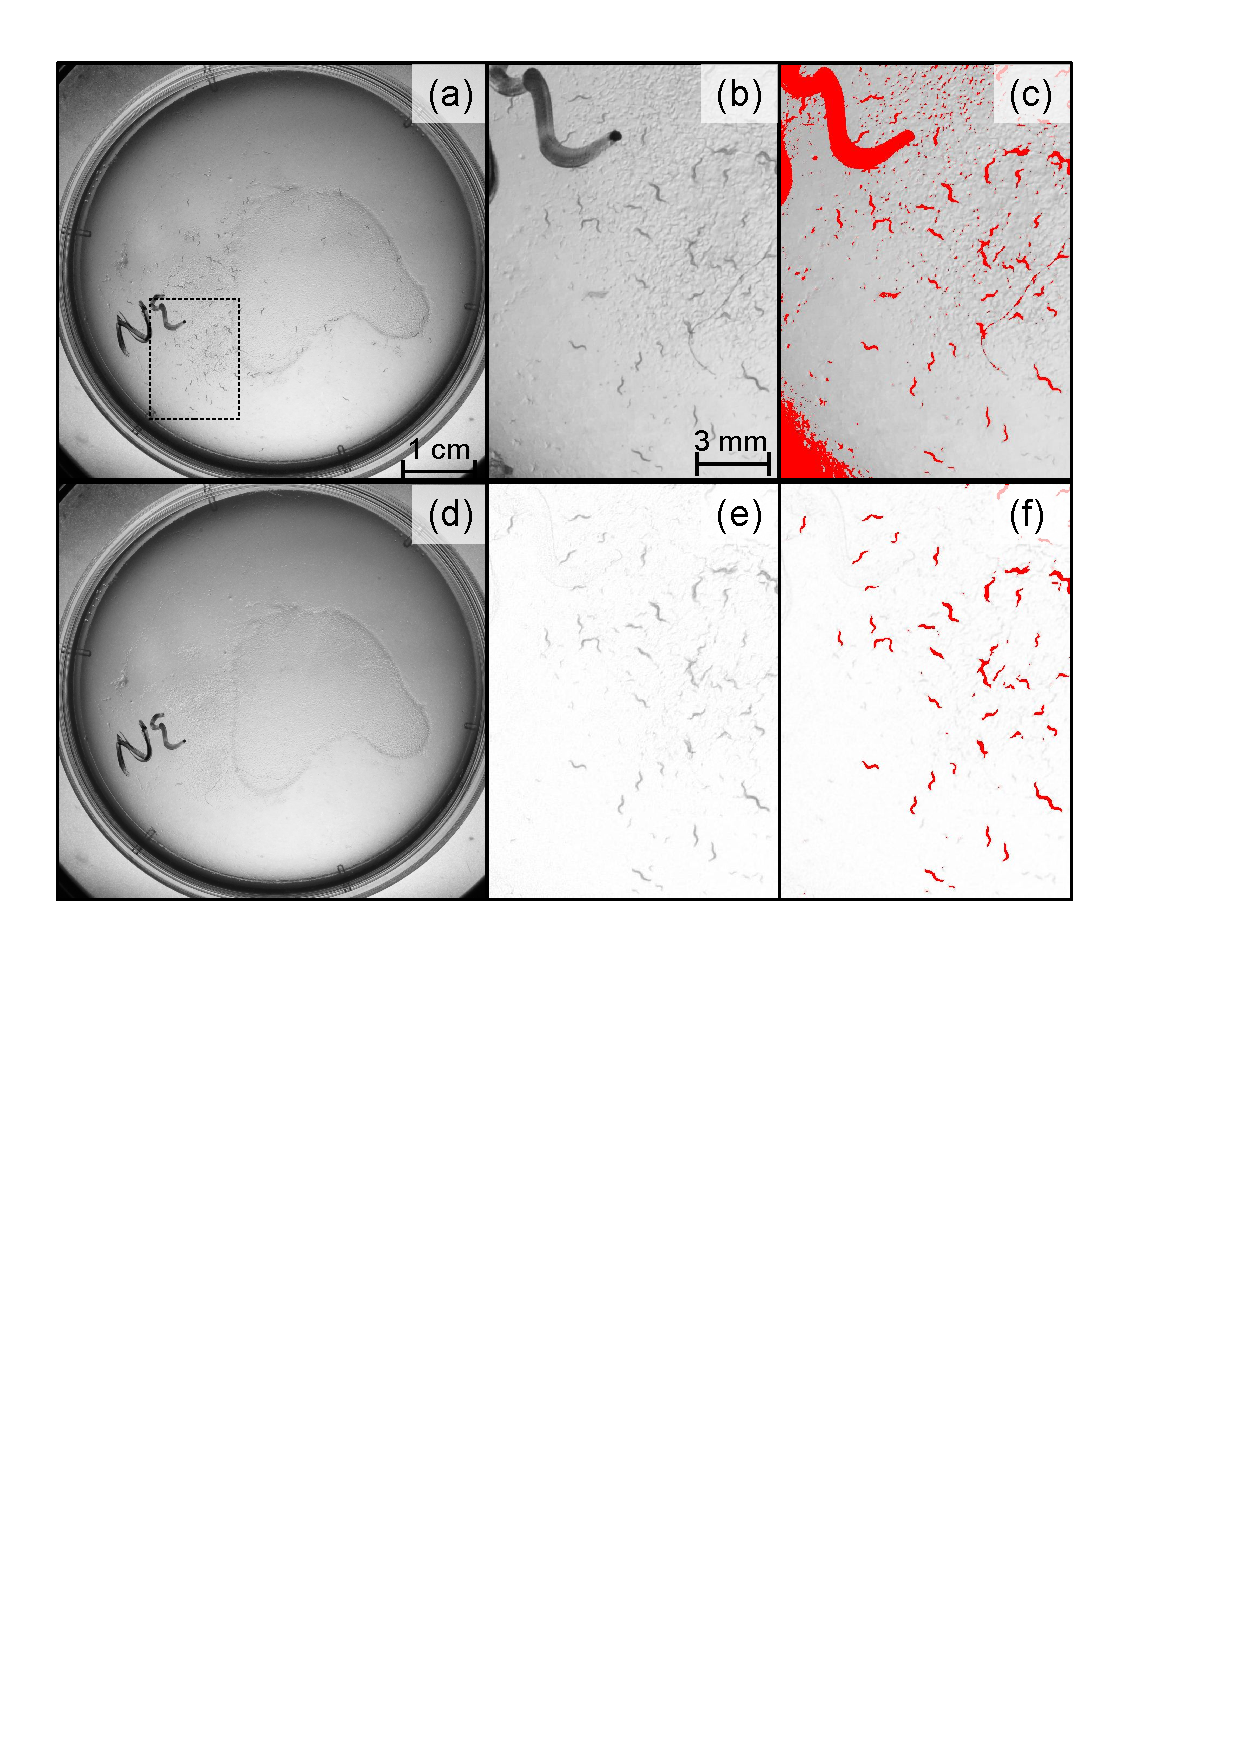
\includegraphics[width=0.95\textwidth]{2_Methodo/Fig/2_Nematodes.pdf} 
\caption[\lofimage{2_Methodo/Fig/2_Nematodes.pdf} Detecting nematodes on agar in a Petri dish]{
Detecting nematodes on agar in a Petri dish. Several pictures of a standard
nematode rearing plate such as (a) have been taken. From this stack of pictures,
a background image (d) has been created. The four other panels are close-up
views of the same area (dashed rectangle of (a)) before (b, c) and after (e,f)
the removal of the background image. A standard particle analysis run on the
original pictures (b,c) failed to bring out only the nematodes: an optimal
thresholding is impossible because of the background heterogeneity (c). But
removing the still background (e) allows a much more efficient detection of the
nematodes (f).}
\label{Fig21-2}
\end{figure}

\subsubsection{Counting and identifying pond copepods and ostracods}

The method has also been applied for detecting zooplankton (\textit{Daphnia} \&
\textit{Cypris}) in a sample of pond water containing some filamentous algae
(Figure \ref{Fig21-3}a,b). We used the same camera and lighting unit as in the case of the collembolan population.
In order to generate the background image five coloured pictures (interspaced at
app. 5 to 10 sec) have been compared (Figure \ref{Fig21-3}c).

\begin{figure}[!h] % Figure 3 
\centering
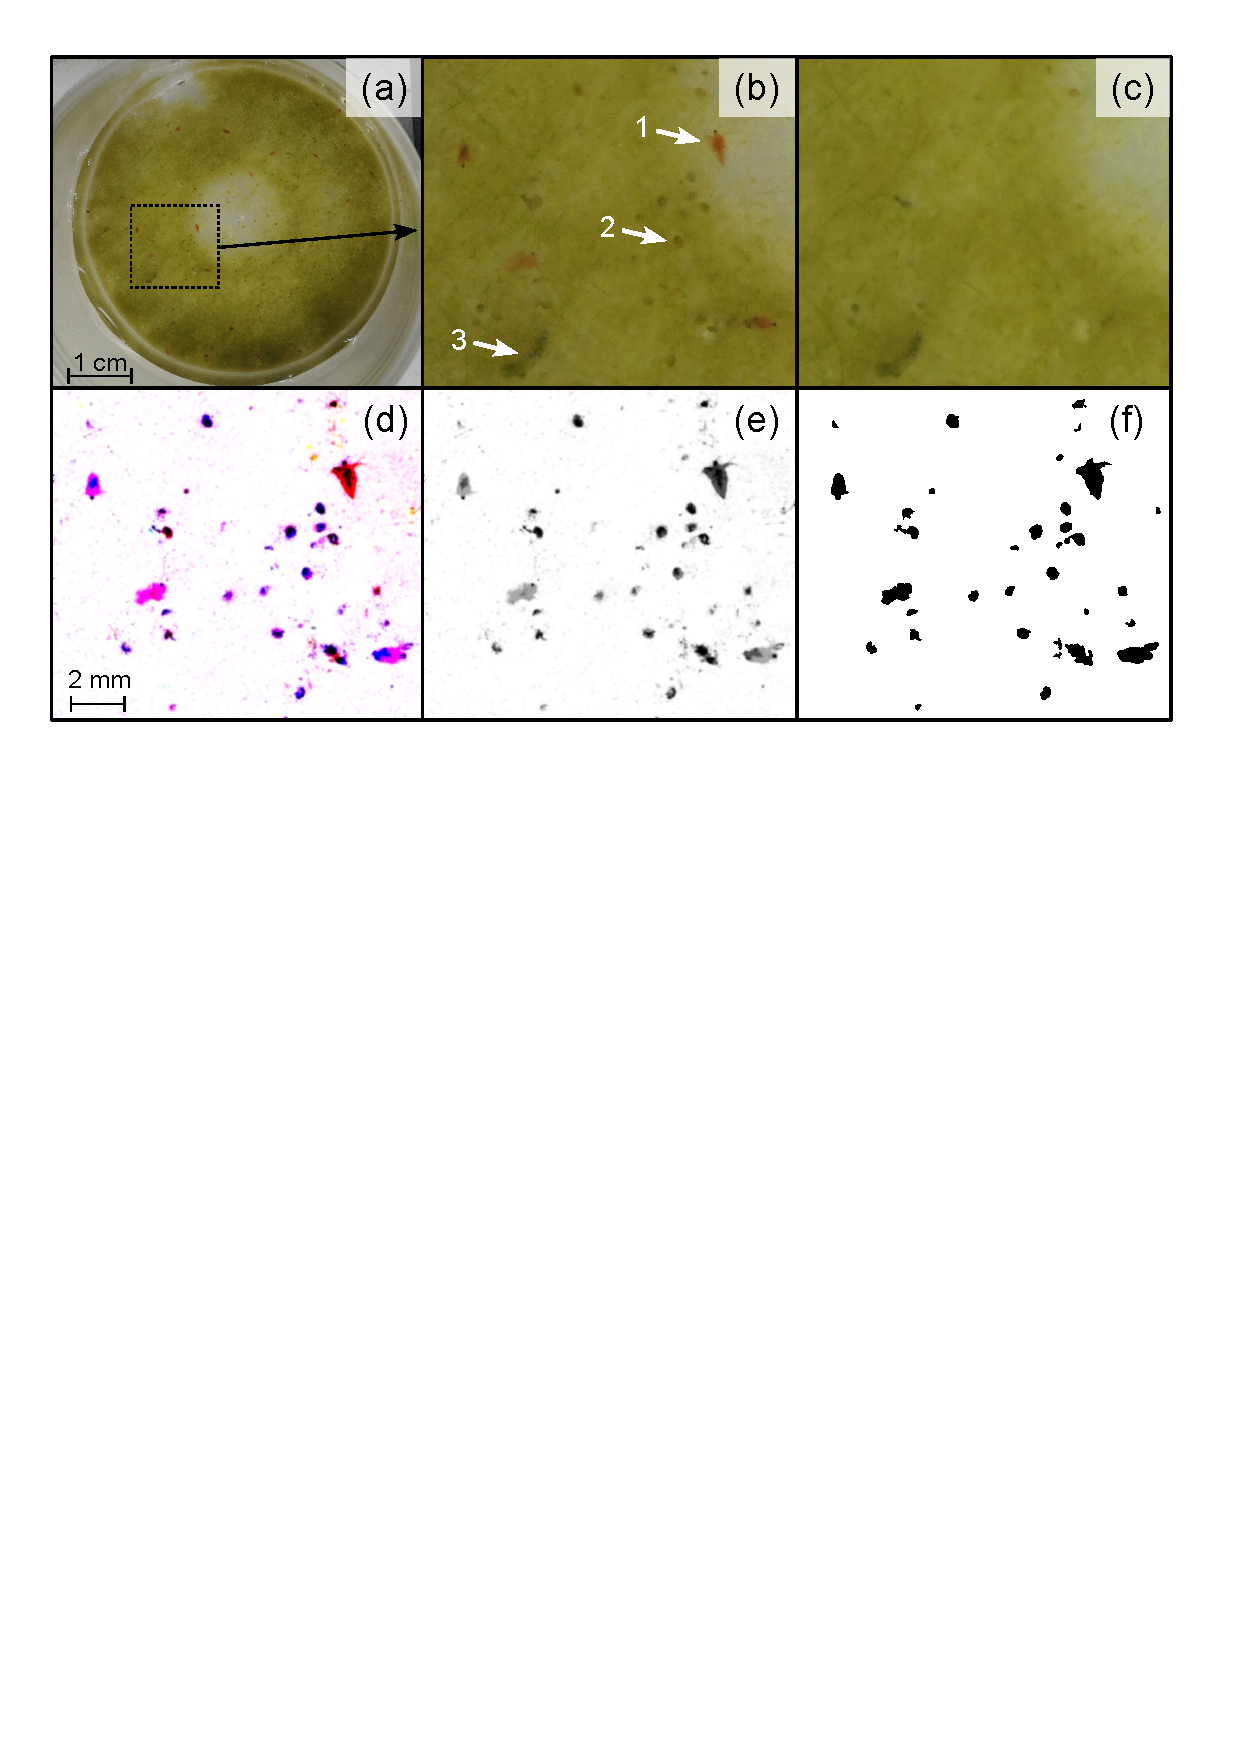
\includegraphics[width=0.95\textwidth]{2_Methodo/Fig/3_Daphnies.pdf} 
\caption[\lofimage{2_Methodo/Fig/3_Daphnies.pdf} Detecting and counting the zooplankton in a sample of pond water]{ Detecting and counting the zooplankton in a sample of pond water. (a) One
picture among five similar ones. (b) A close-up view (dashed rectangle) reveals
a few Cladoceran (red \textit{Daphnia}, arrow 1) and several small Ostracods (\textit{Cypris} sp.,
arrow 2) on a layer of green algae. The difference between (b) and still
background (c) reveals the particles that have moved, i.e. the crustaceans. This
picture can be transformed into an 8-bit grey image (e) which can be used to
detect, measure and count the zooplankton (f). The immobile dark clumps (arrow
3) are excluded from the census. The colour image (d) can also be used to
identify different species.}
\label{Fig21-3}
\end{figure}

\subsubsection{Tracking the movements of an isolated collembola}

In this example, we put a single collembola into a container made of three
connected square compartments filled with a substrate of humid and darkened
plaster and track its exploratory behaviour (Figure \ref{Fig21-4}). Two hundred pictures of
the box were taken, one every 5 sec. The lighting unit used was similar to that
previously described for the collembola system.

\begin{figure}[!h] % Figure 4 
\centering
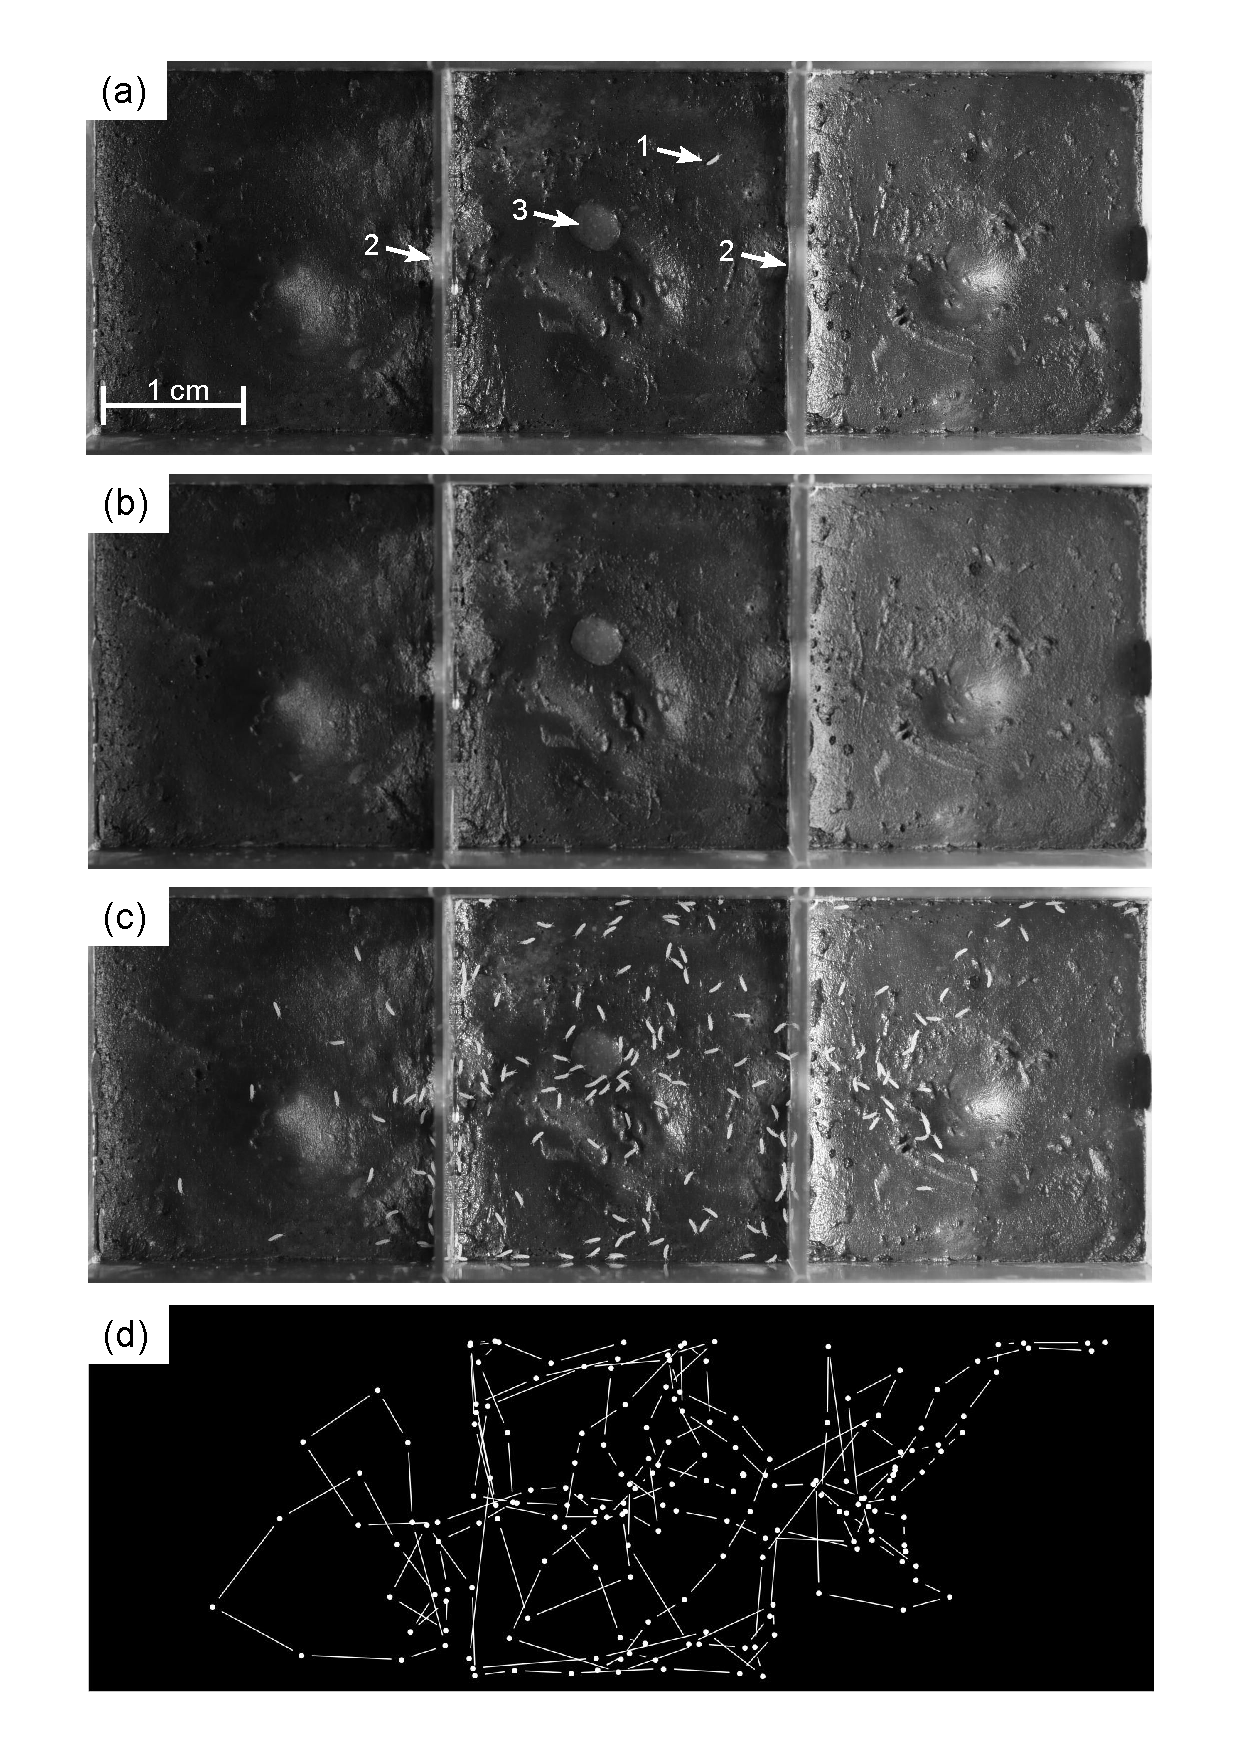
\includegraphics[height=0.75\textheight]{2_Methodo/Fig/4_TrackCollemboles.pdf}
\caption[\lofimage{2_Methodo/Fig/4_TrackCollemboles.pdf} Tracking an isolated collembolan wandering in a container]{ Tracking an isolated collembolan wandering in a container. The container is made of three compartments connected by small holes (arrows 2). A
pellet of food (arrow 3) is visible. A picture was taken every 5 sec. during 30
min. The still background (b) was calculated by averaging the 300 pictures. It
was then then subtracted from each picture to reveal the collembolan. Picture
(c) is the addition of the background (b) and of all the images after the
background's removal. It shows the different positions of the collembola during
the follow-up. The full track of the springtail is plotted on panel (d).}
\label{Fig21-4}
\end{figure}

\subsubsection{Measuring the temporal dynamics of activity in an ant colony}

A high resolution usb webcam (Dinolite AM7013MZT, 5 Mp) was placed above a
laboratory ant colony (Figure \ref{Fig21-5}a) continuously lit by a LED bulb. The camera was
programmed to capture an image of the nest entrance (Figure \ref{Fig21-5}, arrow 1) every 30
sec during 18 hours. The $\approx$2000 images have then been processed with ImageJ in
order to compute the fixed background. The number of ants wandering around the
nest were then automatically counted on each picture (Figure \ref{Fig21-5}d).

\begin{figure}[!h] % Figure 5 
\centering
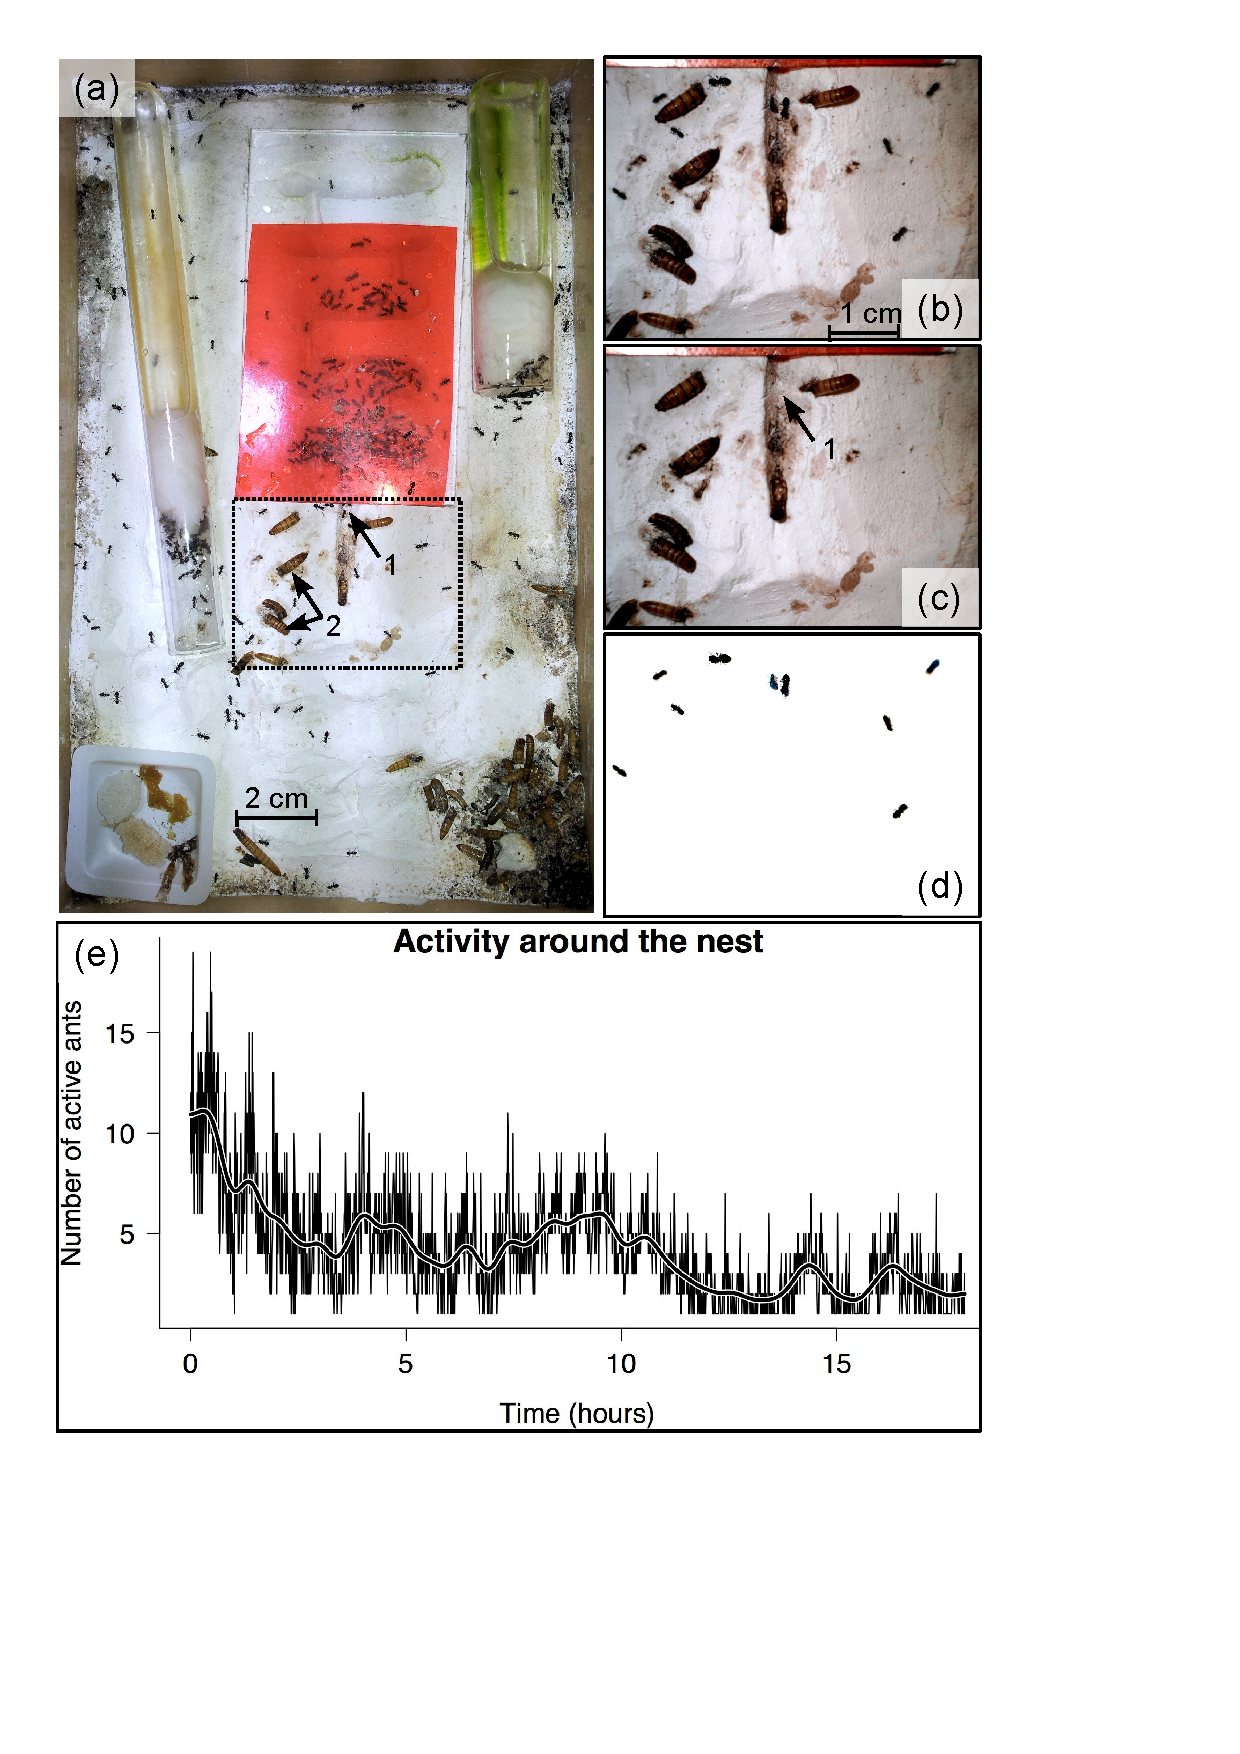
\includegraphics[height=0.60\textheight]{2_Methodo/Fig/5_Fourmis.pdf} 
\caption[\lofimage{2_Methodo/Fig/5_Fourmis.pdf} Follow-up of the activity of an ant colony]{ Follow-up of the activity of an ant colony. (a) General view of an ant colony
bred in the laboratory on a plaster substrate. The below-ground colony is under
the red plastic slate. The ants activity around the nest entrance (arrow 1) has
been followed within the dashed rectangle (b). (c) The background image is built
up through the comparison of multiple pictures (median value). (d) The
difference between (b) and (c) reveals the ants entering and exiting the nest.
Immobile dark particles such as remains of food (Tenebrio larvae, arrow 2) are
discarded from the analysis. (e) By automatically repeating the previous steps,
one can easily count the number of active ants around the entrance of the nest.
This has been done every 30 sec for 18 h. The graph displays all these
measurements and reveals the temporal dynamics of the mean activity around the
nest.
}
\label{Fig21-5}
\end{figure}


\subsection{Method reliability}

\subsubsection{How many pictures are needed ?}

We studied the minimal number of images needed according to particle density,
using springtail populations as an example (Figure \ref{Fig21-1}). We took sets of twenty
pictures of ten rearing boxes with increasing densities of juveniles measuring
$\approx$0.15 to 0.5 mm long. For each density, we performed our analysis on different
subsets of the whole set of pictures, progressively increasing the number of
images used to calculate the background (Figure \ref{Fig21-6}a). A total of 320 sets of
pictures were analysed.

\begin{figure}[!h] % Figure 6 
\centering
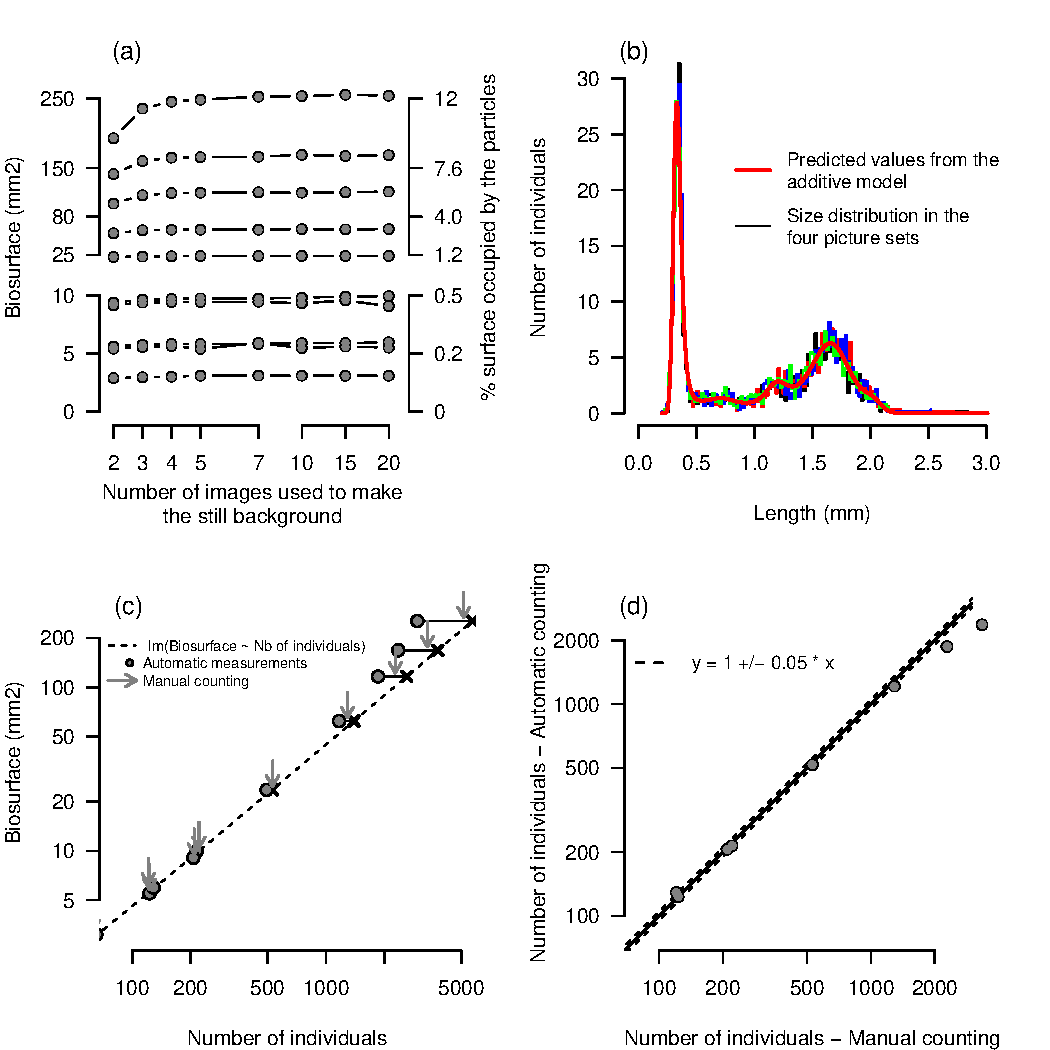
\includegraphics[width=0.90\textwidth]{2_Methodo/Fig/6_Plugin_multiP.pdf}
\caption[\lofimage{2_Methodo/Fig/6_Plugin_multiP.pdf}  Assessing the method's reliability on a collembola population]{ Assessing the method's reliability on a collembola population. (a) Total measured collembolan biosurface (mm2) depending on the number of pictures
in the stack. For low densities, two or three pictures are sufficient to have a
good and reliable measurement. For higher densities, four or five pictures are
needed. (b) Size distribution of the same collembola population. Four different
sets of pictures taken by two different users were analysed. The size classes
are 0.02 mm width. We fitted a generalised additive model that did not show any
significant difference between the pictures nor between the sets. (c-d)
Reliability of the automatic counting method. (c) The estimated biosurface
measured in 10 boxes and the number of individuals automatically counted
(circles). Results of the manual counting are shown (grey arrows) together with
a linear regression between the biosurface and the number of individuals
calculated for the five lowest density boxes. (d) Comparison of the number of
individuals for automatic and manual counting methods.
}
\label{Fig21-6}
\end{figure}

\subsubsection{How repeatable are the measurements of a population structure?}

To illustrate the repeatability of the method for measuring a population
structure, we analysed four sets of five or six pictures of the same collembolan
population (Figure \ref{Fig21-6}b). We divided the size distribution of collembolan (from
0.1 to 3 mm) into 145 classes, each of 0.02 mm width, and analysed the number of
individuals in these classes using a generalised additive model (GAM, function
gam of the mgcv library in R) with a Poisson distribution, a cubic regression
spline, and an imposed high number of knots (k=20) to fit the data closely. We
then tested differences between the pictures and the stacks of images using
anova and Chi-squared tests.

\subsubsection{Are the counting measurements reliable?}

To test whether our counting method is reliable, we compared - for several
collembolan densities - the number of particles automatically counted using the
background removal method with a measurement made manually. Ten sets of 20
pictures each were analysed automatically to measure the mean number of
particles and their total surface. The number of individuals was also measured
manually on one picture belonging to each set (Figure \ref{Fig21-6}c-d). We then performed a
linear regression between the surface and the number of individuals calculated
for the five lowest density boxes. The analyses were all implemented in R 2.15.2
software (\url{http:// cran.r-project.org}, \citealp{ihaka1996a}).

\subsection{Automated implementation}

We present an ImageJ plugin called BP\_sensor for “Batch population sensor” that
we have developed to automate the measurements of size and structure in many
replicated laboratory populations raised in experimental microcosms (Figure \ref{Fig21-S1}
in Section \ref{21-SM1}). This plugin was specifically designed to track populations of the
Collembola \textit{Folsomia candida} but it is versatile enough to be easily adapted to
other experimental setups (Figure \ref{Fig21-S2} in Section \ref{21-SM1}). It automatically performs the
recursive census of multiple laboratory populations of collembolans (Figure \ref{Fig21-S3}
in Section \ref{21-SM1}). The code is written in Java and runs within the freely available
and open-source ImageJ software (\citealp{abramoff2004a}, 
\url{http://rsbweb.nih.gov/ij/}).
% We
% provide in the Supporting Information the commented Java code (File S2) that can
% be directly compiled and run with ImageJ as well as a set of image examples
% (File S3) and some explanations (Section \ref{21-SM1}) to help understand how it works and
% how it can be customised (see Table \ref{Tab21-1} in Section \ref{21-SM1}).

\section{Results and discussion}

\subsection{Counting and tracking individuals in various biological systems}

The method we propose allows a standardisation and automation of microcosm
measurements. The segmentation of pictures into regions of interest that match
structural units is one of the most critical steps in the process of reducing
the complexity of images and extracting information \autocite{russ2002a}. It
usually relies on efficient and precise thresholding. When a single picture is analysed without
making use of our background removing procedure, the efficiency of this crucial
thresholding step can be improved by (1) controlling the overall luminosity to
ensure selecting particles with the same precision everywhere on the picture
(homogeneous lighting) and by (2) maximising the contrast between the particles
(here living organisms) and their background (here substrate) to get a straight
particle segmentation. Removing the motionless background corrects for
heterogeneity in lighting conditions and in the underlying substrate. In Figure
\ref{Fig21-4}, the blackness of the substrate is heterogeneous on the original
pictures which would hinder a standard particle analysis to operate efficiently. This
background removal method is also a way to suppress motionless particles and to
increase the contrast between moving particles and their substrate (Figure
\ref{Fig21-1}c,f). It then becomes possible to automatically adjust the
threshold value required for particle measurements since a larger range of the thresholding values will give similar results.

This increased robustness comes at a cost: the multiple pictures have to be
perfectly lined up. Even a slight movement can blur the constructed background
image and the rest of the analysis will fail. That is why we recommend using a
stable stand and a remote shutter release to avoid any movement of the camera.
Note that it is possible to translate and re-align images that have moved using
the multiplication of the Fourier transformed images (convolution). Our method
is also sensitive to temporal luminosity variations: the moving particles can
create shadows that darken their surrounding substrate, which locally reduces
the efficiency of the background removal. Providing omnidirectional and stable
lighting limits the formation of shadows and easily avoids these unwanted
effects.

On 8-bit grey images, the background image can either be calculated as the
maximum or the minimum grey value in the stack, depending on whether the moving
particles are lighter or darker than their substrate. In our case study, the
springtails are lighter than the darkened plaster and we used the minimal value.
However, using the median or the mean value can be advantageous, especially when
the background is very heterogeneous or the contrast between the particles and
the substrate is so small that the moving elements can be either darker or
lighter than the substrate depending on their positions. For these reasons, we
used the mean grey value to calculate the background in all four additional
examples. To be efficient, the number of analysed and compared pictures has to
be relatively high (at least 4 or 5). Similarly, it is often more efficient to
remove the background by computing the “difference” between the original images
and the background rather than simply the “subtraction” (see the options of the
ImageJ “Image calculator” function). Here we applied this method to extract the
nematodes from their background as they were either brighter or darker than
their agar substrate, depending on the local light reflection.

Given a few adjustments, our measurement method can be applied to various
systems. It was quite efficient at highlighting nematodes on agar. Removing the
background (Figure \ref{Fig21-2}d) improved the reliability for the detection of nematodes
(Figure \ref{Fig21-2}b,c and f) even though the image was faintly contrasted (Figure \ref{Fig21-2}e).
Although it improved the detection of adults, the analysis was not perfect
since, for example, the small worms were not detected (Figure \ref{Fig21-2}). But the use of
a more performant and homogenous lighting unit, combined with some additional
image processing such as smoothing, could certainly improve the analysis
efficiency.

In the pond water sample (Figure \ref{Fig21-3}), the “substrate” is not motionless: the
swimming organisms can shake or move the algae or non living fragments floating
around, which can alter the process of background removal. But despite this
potential drawback, the method turned out to be pretty efficient at bringing out
the zooplankton. It even managed to reveal minor morphological details which
were almost hidden in the original pictures (cf. antenna of the \textit{Daphnia} pointed
by arrow 1 on Figure \ref{Fig21-3}c). However, long term tracking (as for the ant colony or
an isolated springtail) would probably fail owing to too much long term blurring
of the background – unless several backgrounds are recursively constructed on a
shifting subset of the whole stack of images.

Figure \ref{Fig21-4} illustrates how this method can be used to easily track the movement
and behaviour of an individual exploring an heterogeneous landscape (cf.
multi-tracker plugin \citealp{kuhn2001a}). The ant activity around the nest is
also an interesting application example. We did not track through time a constant number
of moving particles nor census a complete population but counted individuals in
a partial area of the colony on a long time scale (18h). The entire data were
then grouped on a diagram in order to show the temporal dynamics of the colony’s
activity near the nest entrance (Figure \ref{Fig21-5}). We do not compare the results
obtained with manual measurements that would be very time consuming. However,
the activity measurements are coherent with an initial increased activity, no
doubt caused by disturbance during the setting up of the experiment (Figure \ref{Fig21-5}e):
the second half of the measurements were done at night and this could explain
the decrease of activity.

For both the pond water sample (Figure \ref{Fig21-3}) and the ant colony (Figure \ref{Fig21-5}), the
processing was done on coloured pictures. This provided interesting additional
information since the colour remained after removal of the background. This
information could be used together with the size and shape of the particles to
help identify, for instance, different species (here \textit{Daphnia} \& \textit{Cypris}, Figure
\ref{Fig21-3}d). Such colour images could also benefit from some specific
treatment such as decorrelation stretch (DStretch imageJ plugin) to bring out the different
particles of interest \autocite{harman2011a}.

\subsection{Testing the method’s reliability in an optimised acquisition system}

\subsubsection{Background calculation - Number of pictures needed}

The reliability of the method relies on the quality of the still background
image, which has to be free from any moving particle. This will depend on the
number of images compared to make the background and on the proportion of the
substrate occupied by the creatures. If their density is high, more images are
needed for each pixel of the substrate to be visible on at least one image. The
replicated analysis performed with increasing number of images in a single stack
showed that the total measured biosurface increases with the number of pictures
analysed (Figure \ref{Fig21-6}a). But for low densities (0 to 250 individuals - which
corresponds to a biosurface of 3 to 10 mm2, the rearing box surface measuring 20
cm2), this increase is almost negligible. For these low densities, the
probability that part of the substrate is covered by a collembola on more than
one picture is very low. Taking more than two pictures does not really improve
the reliability of the measurements. But for higher densities, three, four or
five pictures are needed to reveal the whole background substrate which is
needed for reliable and robust estimation of the population biosurface. In our
study case, taking more than five pictures never improved the measurement
reliability. As a rule, comparing four pictures ensures reliable measurements.

\subsubsection{Repeatability of a population structure measurement}

The estimation of the population structure was repeatable (Figure \ref{Fig21-6}b): the four
estimated size distributions were largely overlapping. A fitted generalised
additive model to these distributions explains most of the variance (84\%) and
we found that the estimated size distributions did not differ between the
different sets of pictures ($\gamma ^2_3$=2.3, p=0.5), nor between the different
pictures within each set ($\gamma^2_{22}$=23.2, p=0.4).

\subsubsection{Reliability of the counting measurement}

The reliability of automatic measurements is good for densities below 1000
individuals, but beyond this density the automatic counting underestimates the
density (controlled manually):  more and more individuals adjoin each other and
are then detected as one large particle (Figure \ref{Fig21-6}d). The measured total
biosurface then becomes a better proxy for the number of individuals in the box:
a projection of the biosurface values of the five highest densities on the
linear regression provides a less biased density estimate (Figure \ref{Fig21-6}c). But this
correction only works if the individuals have similar size and if they do not
overlap, which is the case here. A more complex particle image analysis, like
the watershed algorithm \autocite{vincent1991a} could also be used to split up
merged individuals.

\subsection{Automated implementation}

We have developed an automatic measuring and counting procedure using multiple
picture analyses that is easy to use and requires very few calibrations (see
ESM). It takes about two hours to obtain five pictures of a hundred populations
and to manually sort these pictures in a normed directory tree on the computer.
It then takes about one hour for the plugin to analyse these 500 images, count
and measure all the individuals in these populations and save the data in
distinct files (20 to 30 sec per set of 5 pictures on a 2.5GHz computer).
Altogether about three hours are needed to take a census of one hundred
laboratory populations, whose densities can reach a thousand individuals.

One of the major improvements would be to use colour pictures instead of black
and white ones. It would not change the background image calculation but would
allow more complex segmentation of the particles.

\section{Conclusion}

This simple method is easy to implement and proved to be a useful if not
essential image processing step before running a particle detection function.
This method is efficient at removing most of the motionless background and to
correct for spatially heterogeneous lighting conditions. It is sensitive to even
slight movements of the frame or to minor temporal variations in light
intensity. It can be used both on grey-level and coloured pictures. It can be
applied to many laboratory organisms and to various microcosms. Its
implementation has been incorporated into a plugin to automate the analysis of
large batches of images, which we hope will help smoothing and accelerate the
workflow from microcosm experiments to data analysis.

\section{Supplementary material}\label{21-SM1}
\section*{“Batch population
sensor”, an ImageJ plugin to automate the analysis of digital pictures of laboratory
microcosms.}

The plugin BP\_sensor.java automates the successive steps of the analysis and
recursively analyses multiple sets of images, producing rapidly measurements
from a large number of replicated microcosms.

In order to run the ImageJ plugin "BP\_sensor" the following files have to be
saved in the ImageJ plugins folder or a sub-folder thereof : BP\_sensor.java and
Wait\_For\_User.java.

More information on the plugin "Wait for user" can be found on the ImageJ
Documentation Wiki :
\url{http://imagejdocu.tudor.lu/doku.php?id=plugin:utilities:wait_for_user:start}.

Once the files saved, compile first "Wait\_For\_User.java" and then
"BP\_sensor.java" with "Compile and Run". Restart ImageJ, you can now launch the
plugin and follow the instructions. To perform the analysis on the picture set
example provided you need to save them in a given directory that you will be
asked to specify when running the plugin.

As described in the main text, the core of the image processing consists, for
each population, in analysing several pictures of the same microcosm and in
comparing these pictures in order to remove the still background for an enhanced
image segmentation. This process is embedded into other functions to batch
process many stacks of images, scale the measurements, detect the region of
interest in the image where the counting has to be run, adjust the particle
detection threshold and automatically export the data into spreadsheet files
(Table \ref{Tab21-1}).

%\begin{table}
%\centering
\begin{longtable}{
	p{\dimexpr.22\linewidth-2\tabcolsep-1.3333\arrayrulewidth}% column 1
 	p{\dimexpr.78\linewidth-2\tabcolsep-1.3333\arrayrulewidth}}
 	
 	\caption{Overview of the plugin's optional tools}\label{Tab21-1}\\
 	\hline
 	\endhead
%\begin{tabularx}{0.99\textwidth}{
%	p{\dimexpr.2\linewidth-2\tabcolsep-1.3333\arrayrulewidth}% column 1
%  	p{\dimexpr.8\linewidth-2\tabcolsep-1.3333\arrayrulewidth}}
%\caption{Overview of the plugin’s optional tools.}\\
 	
\hline
\endfoot

Pre-treatment 	& Optional smoothing of the pictures before launching the
particle analyses. Two methods are available: the smooth function of ImageJ (average
pixel value in a 3x3 square) or a gaussian blur.\\
\hspace{1cm} &\\
Scaling 		& A pixel-millimetre (or another unit) conversion ratio is estimated
and enables ImageJ to directly measure particles in millimetres. Two methods are
proposed, manual and automatic.\\
\hspace{1cm} &\\
				&- manual: the user is asked to measure a known area and to report its real
value (mm2) and its surface in number of pixels.\\
\hspace{1cm} &\\
				&- automatic: the plugin will automatically detect and measure a contrasted
black rectangle or circle of known size used as reference. An input window will
open to specify (1) the radius length for a circle, the side length for a square
or the mean length of the short and long sides for a rectangle (in mm for
instance). The user will also be asked to specify the approximate position
(pixel coordinates) of the scaling object on the picture as well as the two
extreme values of an interval which is sure to contain this reference area.
Theses parameters will be used by the plugin to search, detect, select and
measure this reference area and to scale the subsequent measurements.\\
\hspace{1cm} &\\
Background calculation & Three calculation methods are proposed to generate the
background picture: minimal (darker), average or median value for this
“z-projection” of the original stack. Note that average or median are preferred
to buffer lighting heterogeneity between the images in the stack, but they
usually require more images to perform well.\\
\hspace{1cm} &\\
Selection of a region of interest & This option is useful if one wants to ensure
that the program will only analyse the particles that are within a specific
region of interest (roi) of the picture. If selected, a new input window will
open to specify its approximate position (pixel coordinates in the image) as
well as the two extreme values of an interval which is sure to contain the
surface area for this roi. The plugin will try to find the larger black region
within this interval size that maximises the circularity. The user is also asked
to supply a minimal circularity value. If no roi is found above this value, the
user will later be asked to manually select the roi.\\
\hspace{1cm} &\\
Particle analysis threshold & The user can choose an automatic thresholding
method, "Intermodes", that assumes a bimodal distribution and fix the threshold
at the mean value of the two local extrema. Alternatively, a fixed threshold
value can be imposed.\\
\hspace{1cm} &\\
Moving particles darker than their substrate & The plugin can invert the
pictures when loading the stack. All the steps will then be performed the same
way. This can be useful if one has dark particles moving on a lighter
background.\\

\end{longtable}
%\end{tabularx}
%\end{table}

The first step is to take successive pictures (ideally three to five) of the
microcosms under study in stable conditions using a camera stand, a remote
shutter release and constant lighting conditions. The different sets of pictures
are to be sorted in a file tree as shown in Figure \ref{Fig21-S1}. When the plugin is
started, one has to specify the location of this file tree and the folder in
which the produced data files will be saved. Then several optional functions can
be activated (Figure \ref{Fig21-S2}). These functions are described in Table \ref{Tab21-1}. Note that
since most of them are written as sub-functions in our java code, they can be
easily modified and customised for other setups. The default values of the input
windows can also be changed in the java code. After each stack measurement,
the results of the particle analysis are saved in a distinct .xls files
(Figure \ref{Fig21-S1}) named after the directory path that contains the analysed pictures.
It is possible in the main option window to specify the number of directory
levels that will be included in the output file names.

\begin{figure}[!h] % Figure S1 
\centering
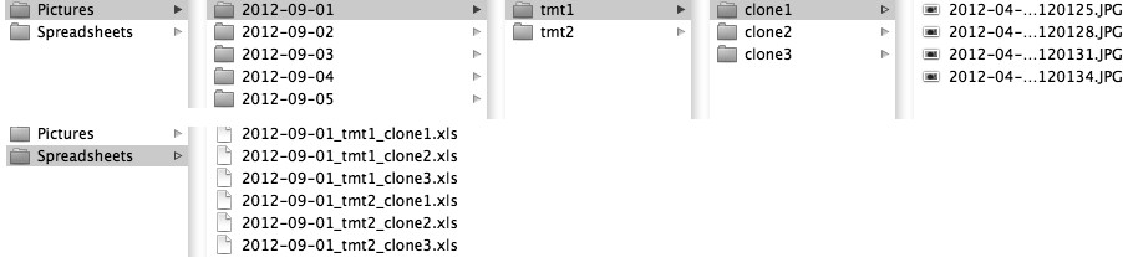
\includegraphics[width=0.95\textwidth]{2_Methodo/Fig/FigS1.pdf}
\caption[\lofimage{2_Methodo/Fig/FigS1.pdf}  Example of a directory tree and
resulting tables]{ Example of a directory tree with sorted pictures (upper part)
and the resulting tables (lower part).
}
\label{Fig21-S1}
\end{figure}

\begin{figure}[!h] % Figure S2 
\centering
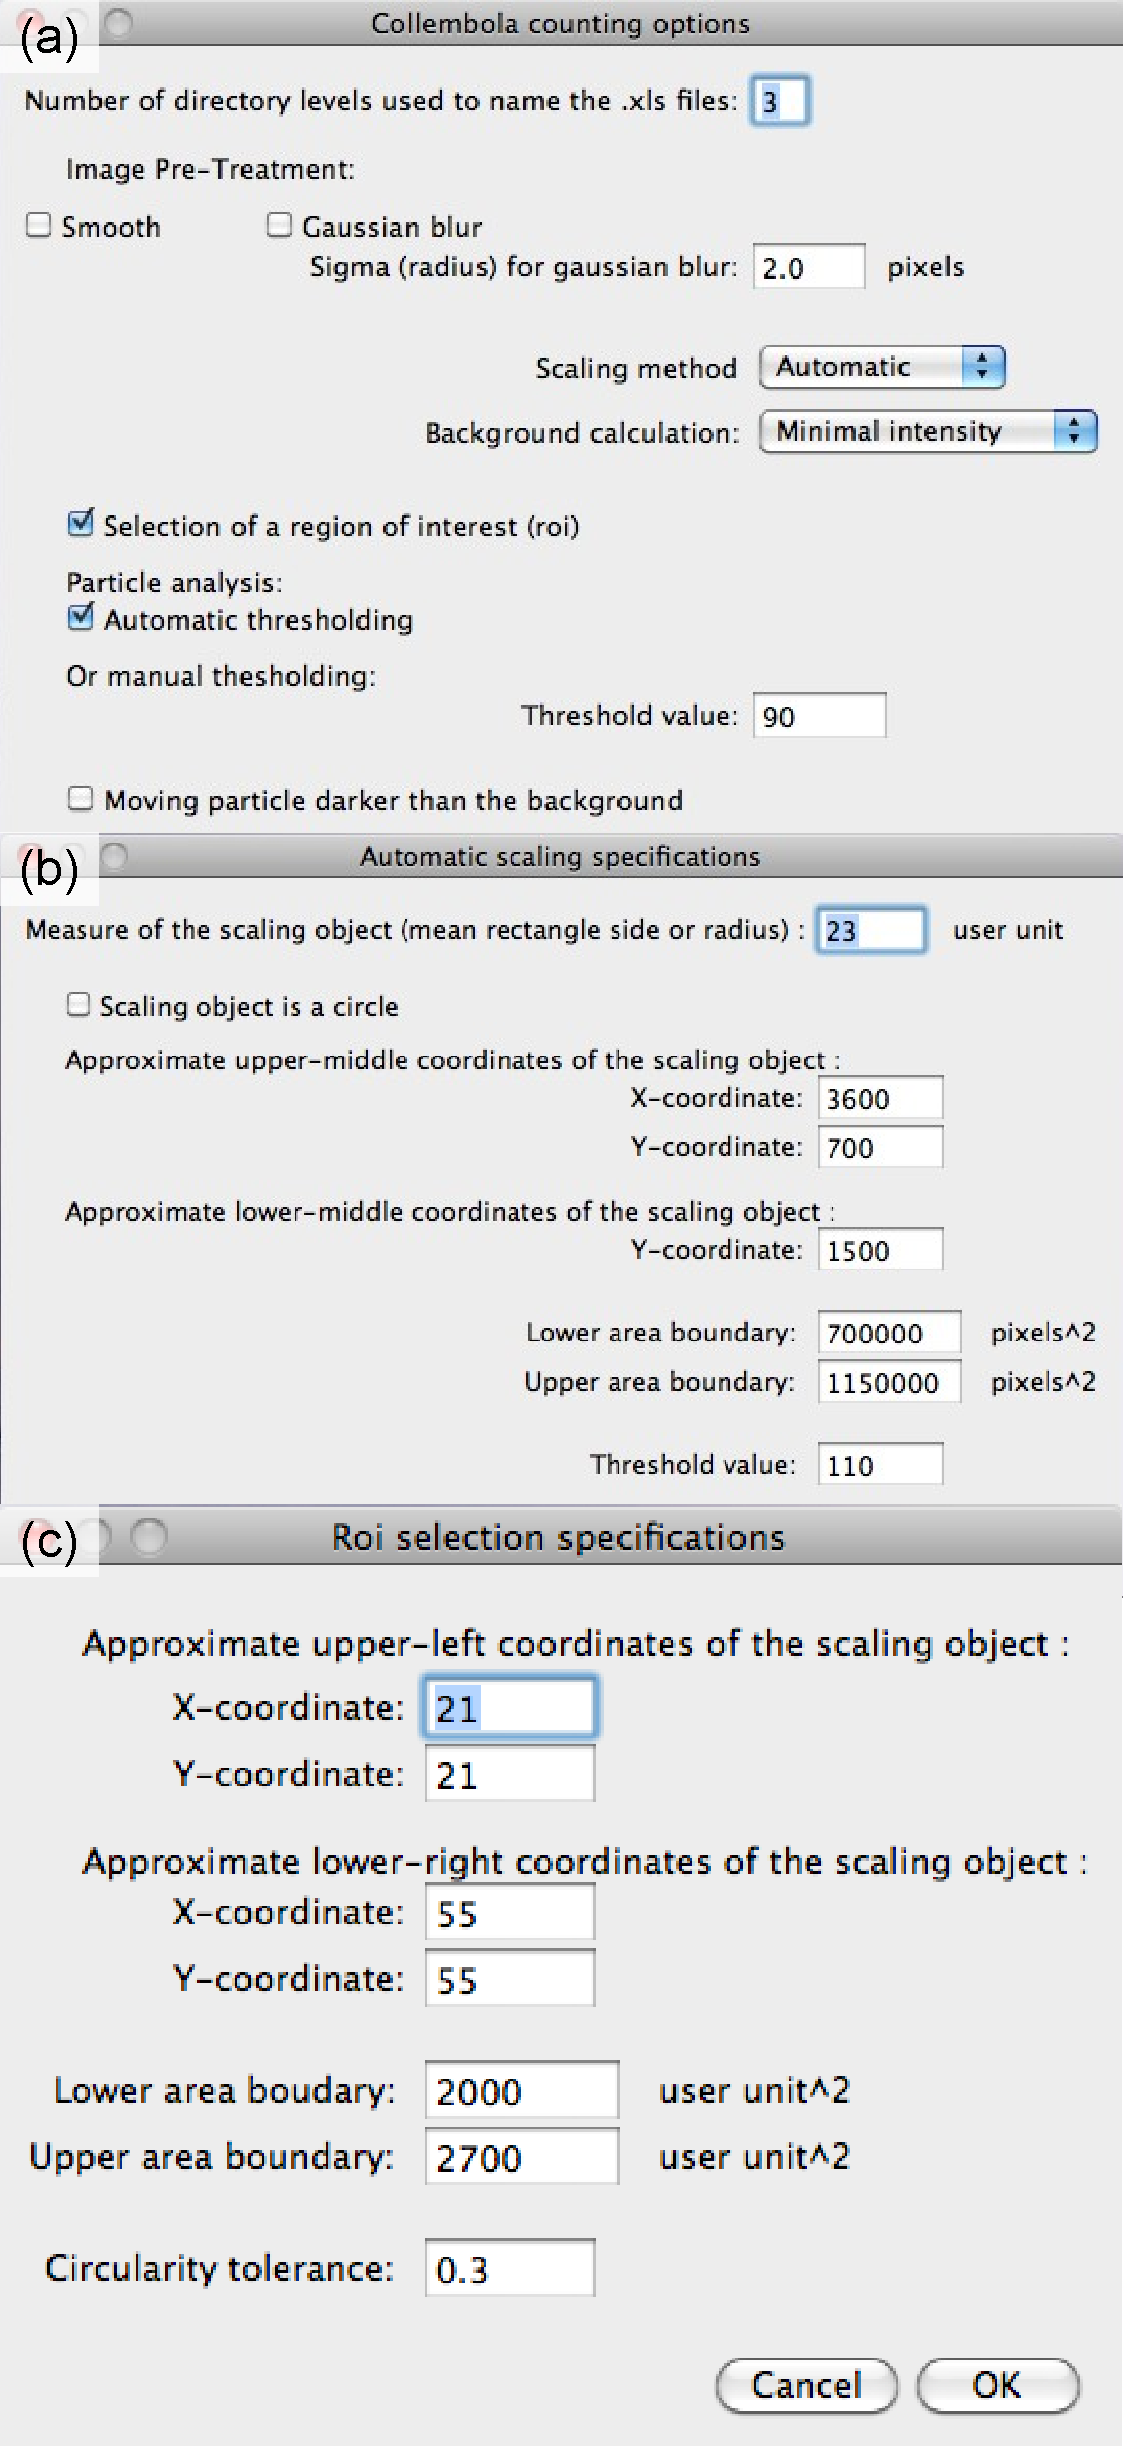
\includegraphics[height=0.85\textheight]{2_Methodo/Fig/FigS2.pdf}
\caption[\lofimage{2_Methodo/Fig/FigS2.pdf}  Plugin specification windows]{ Plugin specification windows. (a) On this window one is asked to specify the variables
described in Table 1. If selected, the automatic scaling specification window
(b) and the region of interest (roi) selection specifications window (c) will
open successively.
}
\label{Fig21-S2}
\end{figure}

As an example, we provide in the supporting material a set of pictures that can
be analysed with our plugin using the default values. The main steps are
illustrated in Figure \ref{Fig21-S3}: the background picture is first constructed (Figure
\ref{Fig21-S3}b) by comparing the different images in the stack (Figure
\ref{Fig21-S3}a), keeping only the minimal values (darker) for each pixel. This background picture is then
removed from the different images of the original stack. It creates a new stack
where only the moving particles remain (Figure \ref{Fig21-S3}d). In this example, the
background image is also used to scale the measurements. A black square on the
top right of the picture (arrow 2) is selected and measured to automatically
convert in mm the future measurements. It is also possible to select a reference
distance (arrow 1) to manually adjust the scale. The plugin will then detect the
boundary of the rearing box (Figure \ref{Fig21-S3}b, arrow 3), and retrieve on the new stack
of images this selected region of interest (Figure \ref{Fig21-S3}d). Within this boundary,
an automatic threshold is applied and the particles are measured and counted
(Figure \ref{Fig21-S3}d) The background removal is an essential step that makes possible the
automation of the thresholding. As shown in Figure \ref{Fig21-S3}, most of the substrate
heterogeneity is removed. Motionless particles or dead organisms are also
excluded from the automatic census (Figure \ref{Fig21-S3}, arrows 4 and 5). Without this
crucial step, a batch processing of large amounts of replicated populations
would not be possible and a threshold would have to be adjusted manually.

\begin{figure}[!h] % Figure S3 
\centering
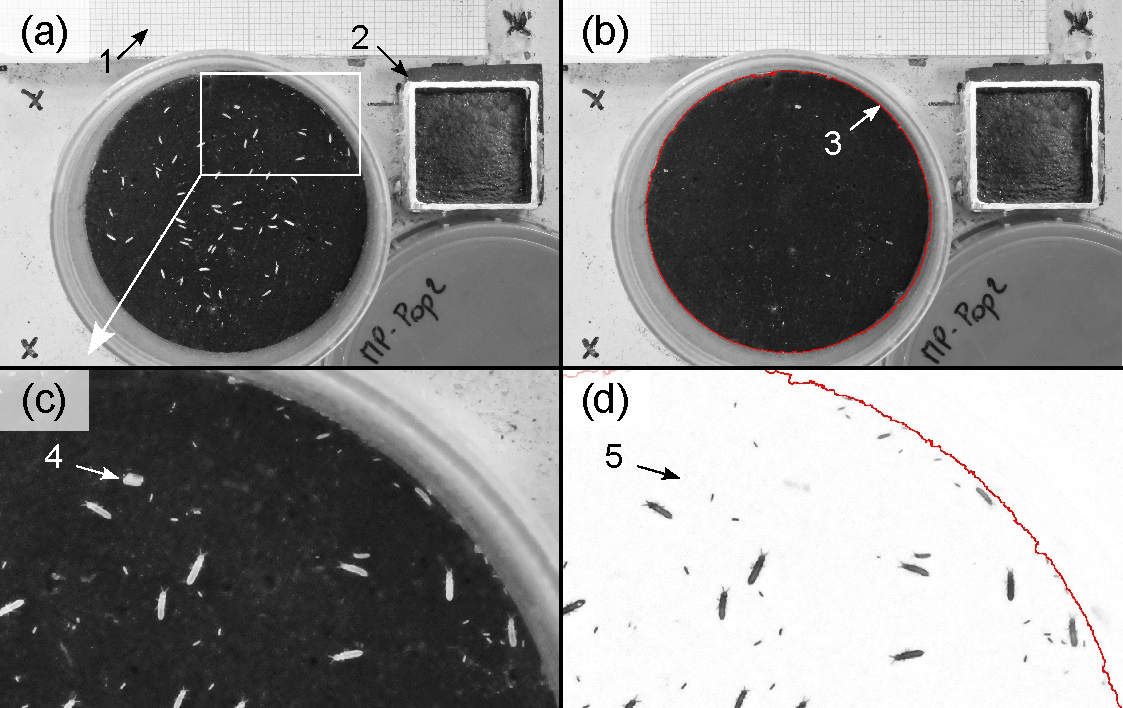
\includegraphics[width=0.95\textwidth]{2_Methodo/Fig/FigS3.pdf} 
\caption[\lofimage{2_Methodo/Fig/FigS3.pdf}Successive steps of the image processing]{
Successive steps of the image processing. (a) Original picture of a rearing box
with its collembola population. A piece of graph paper (arrow 1) and a
contrasted black square (arrow 2) can be used as references to scale the
measurements. (b) By comparing different images, a background picture is
generated: each pixel is the darker pixel of the original set of images. The
white moving collembola are automatically discarded. The border of the box
(arrow 3) is automatically detected and selected by the plugin. (c) Close-up
view of one of the original pictures. Arrow 4 points at a white dirt particle.
(d) Before analysing the particles within the region of interest, the plugin
removes the background which ensures measuring the moving particles only –
motionless white particles or reflections being automatically excluded from the
analysis (arrow 5).}
\label{Fig21-S3}
\end{figure}


Some parts of the provided java code can also be used separately: the automatic
scaling procedure can be used to speed up recursive manual size measurements on
pictures shot at various heights (for example, in field experiments without a
camera stand). One just has to add on each picture, at a relatively constant
position, a contrasted area that can be used for scaling.




\section{Acknowledgments}
We thank Lise Frézal and Marie-Anne Felix for providing the culture of
nematodes, David Carmignac for the \textit{Daphnia} and Romain Peronnet for the ant
colony.
% 
\chapter[Diagramme structure -- temps: remprésentation graphiques de la
dynamique d'une population structurée][Diagramme structure -- temps]{Diagramme structure -- temps: remprésentation graphiques de la
dynamique d'une population structurée}\label{Chap:STDiag}

\vspace{4cm}

\begin{Spacing}{1}
\texttt{
Le Bourlot, Vincent, François Mallard, Caroline Ligier, Manuel Massot, 
David Claessen, and Thomas Tully, "A simple graphical method for 
displaying structured population dynamics and STdiag, its implementation 
in a R package".\\
under review at Journal of Animal Ecology
}
\end{Spacing}

\section*{Abstract}
\addcontentsline{toc}{section}{Abstract}

%\begin{enumerate}
  %\item 
  
  \lettrine[lines=3]{I}{n demography}, a detailed study of the temporal dynamics
  of a population structure is often required to better understand the processes that
  underline the overall dynamics and the individual life histories.
  %\item 
  
  Heatmaps using time and structure (such as size-structure) as x and y
  coordinates and density as colors are efficient tools for displaying the
  dynamics of a structured population. Such representations (structure--time
  diagrams), reveal the data at several levels, from general outlook to fine
  details.
  %\item 
  
  This graphical display is a simple and efficient way to make large
  demographic datasets coherent and to disclose the underlying often hidden
  demographical processes. But despite its efficiency, this method has been
  scarcely used in ecology and demography.
  %\item 
  
  To emphasise how rich this graphical representation is and to illustrate
  that this method can be applied even outside the field of ecology, we present
  three case studies:  a long-term survey of a collembolan population in a
  laboratory microcosm, a 16 years old survey of wild common lizard population and
  the antibiotics consumption in France during one year.
  %\item 
  
  We present the R package STdiag, an interface to complex graphical
  functions to easily produce such "structure--time diagrams" from raw datasets.
  This package available for all operating systems via R-Forge. Its syntax and
  options are described, discussed and illustrated using our three examples.
%\end{enumerate}

\section{Introduction}

Structured populations are complex assemblages of individuals differing in age,
reproductive stage or physiological state such as size or body condition (Figure
\ref{Fig22-1}a, b). Different approaches have been used to display structured
population dynamics (Figure \ref{Fig22-1}c, d, e): By displaying the whole population size fluctuations,
the structure is not taken into account (Figure \ref{Fig22-1}c) \autocite{schrautzer2011a}.
The structure can be roughly considered by splitting individuals into separate
groups (of size or stages) whose dynamics can be displayed on adjacent plots
\autocite{plaistow2009a} or, to facilitate comparisons, on overlaid curves (Figure
\ref{Fig22-1}d) or on a stacked bar plot (Figure \ref{Fig22-1}e) \autocite{madsen2000a}. But condensed
three-dimensional diagrams are required to finely display the structure dynamic
especially when the structuring factor is continuous (size, age). These diagrams
encompass “event history diagrams” that allow the graphical representation of
life history traits at the individual level of a whole
cohort\autocite{carey1998a,carey2008a} or the production of “shaded contour
maps” such as the ones used to represent the temporal dynamics of
aged-structured demographic rates such as death or birth rates in human
populations \autocite{vaupel1997a,vaupel1998a}.These graphical representations
are mainly used in human demography to represent secular changes in
age-dependent demographicrates
\autocite{vaupel1987a,vaupel1997a,vaupel1998a,andreev2000a,erlangsen2003a}.
To our knowledge, despite their interest, such powerful visual displays have
almost never been used in ecology to represent the temporal dynamics of
structured populations \autocite{faerovig2002a}. This may result from the
prohibiting cost of publishing colours pictures. But with the development of
online publishing, colour methods are becoming more widely used.
The R software \autocite{team2012a} is a language and environment for data
manipulation, calculation, statistical computing and graphic display. R provides
libraries such as \texttt{lattice} \autocite{sarkar2008a} or \texttt{ggplot2}
\autocite{wickham2009a} to produce heatmaps.
But although higly customizable, the plotting functions are often difficult to
handle for beginners.

\begin{figure}[!ht] % Figure 1 
\centering
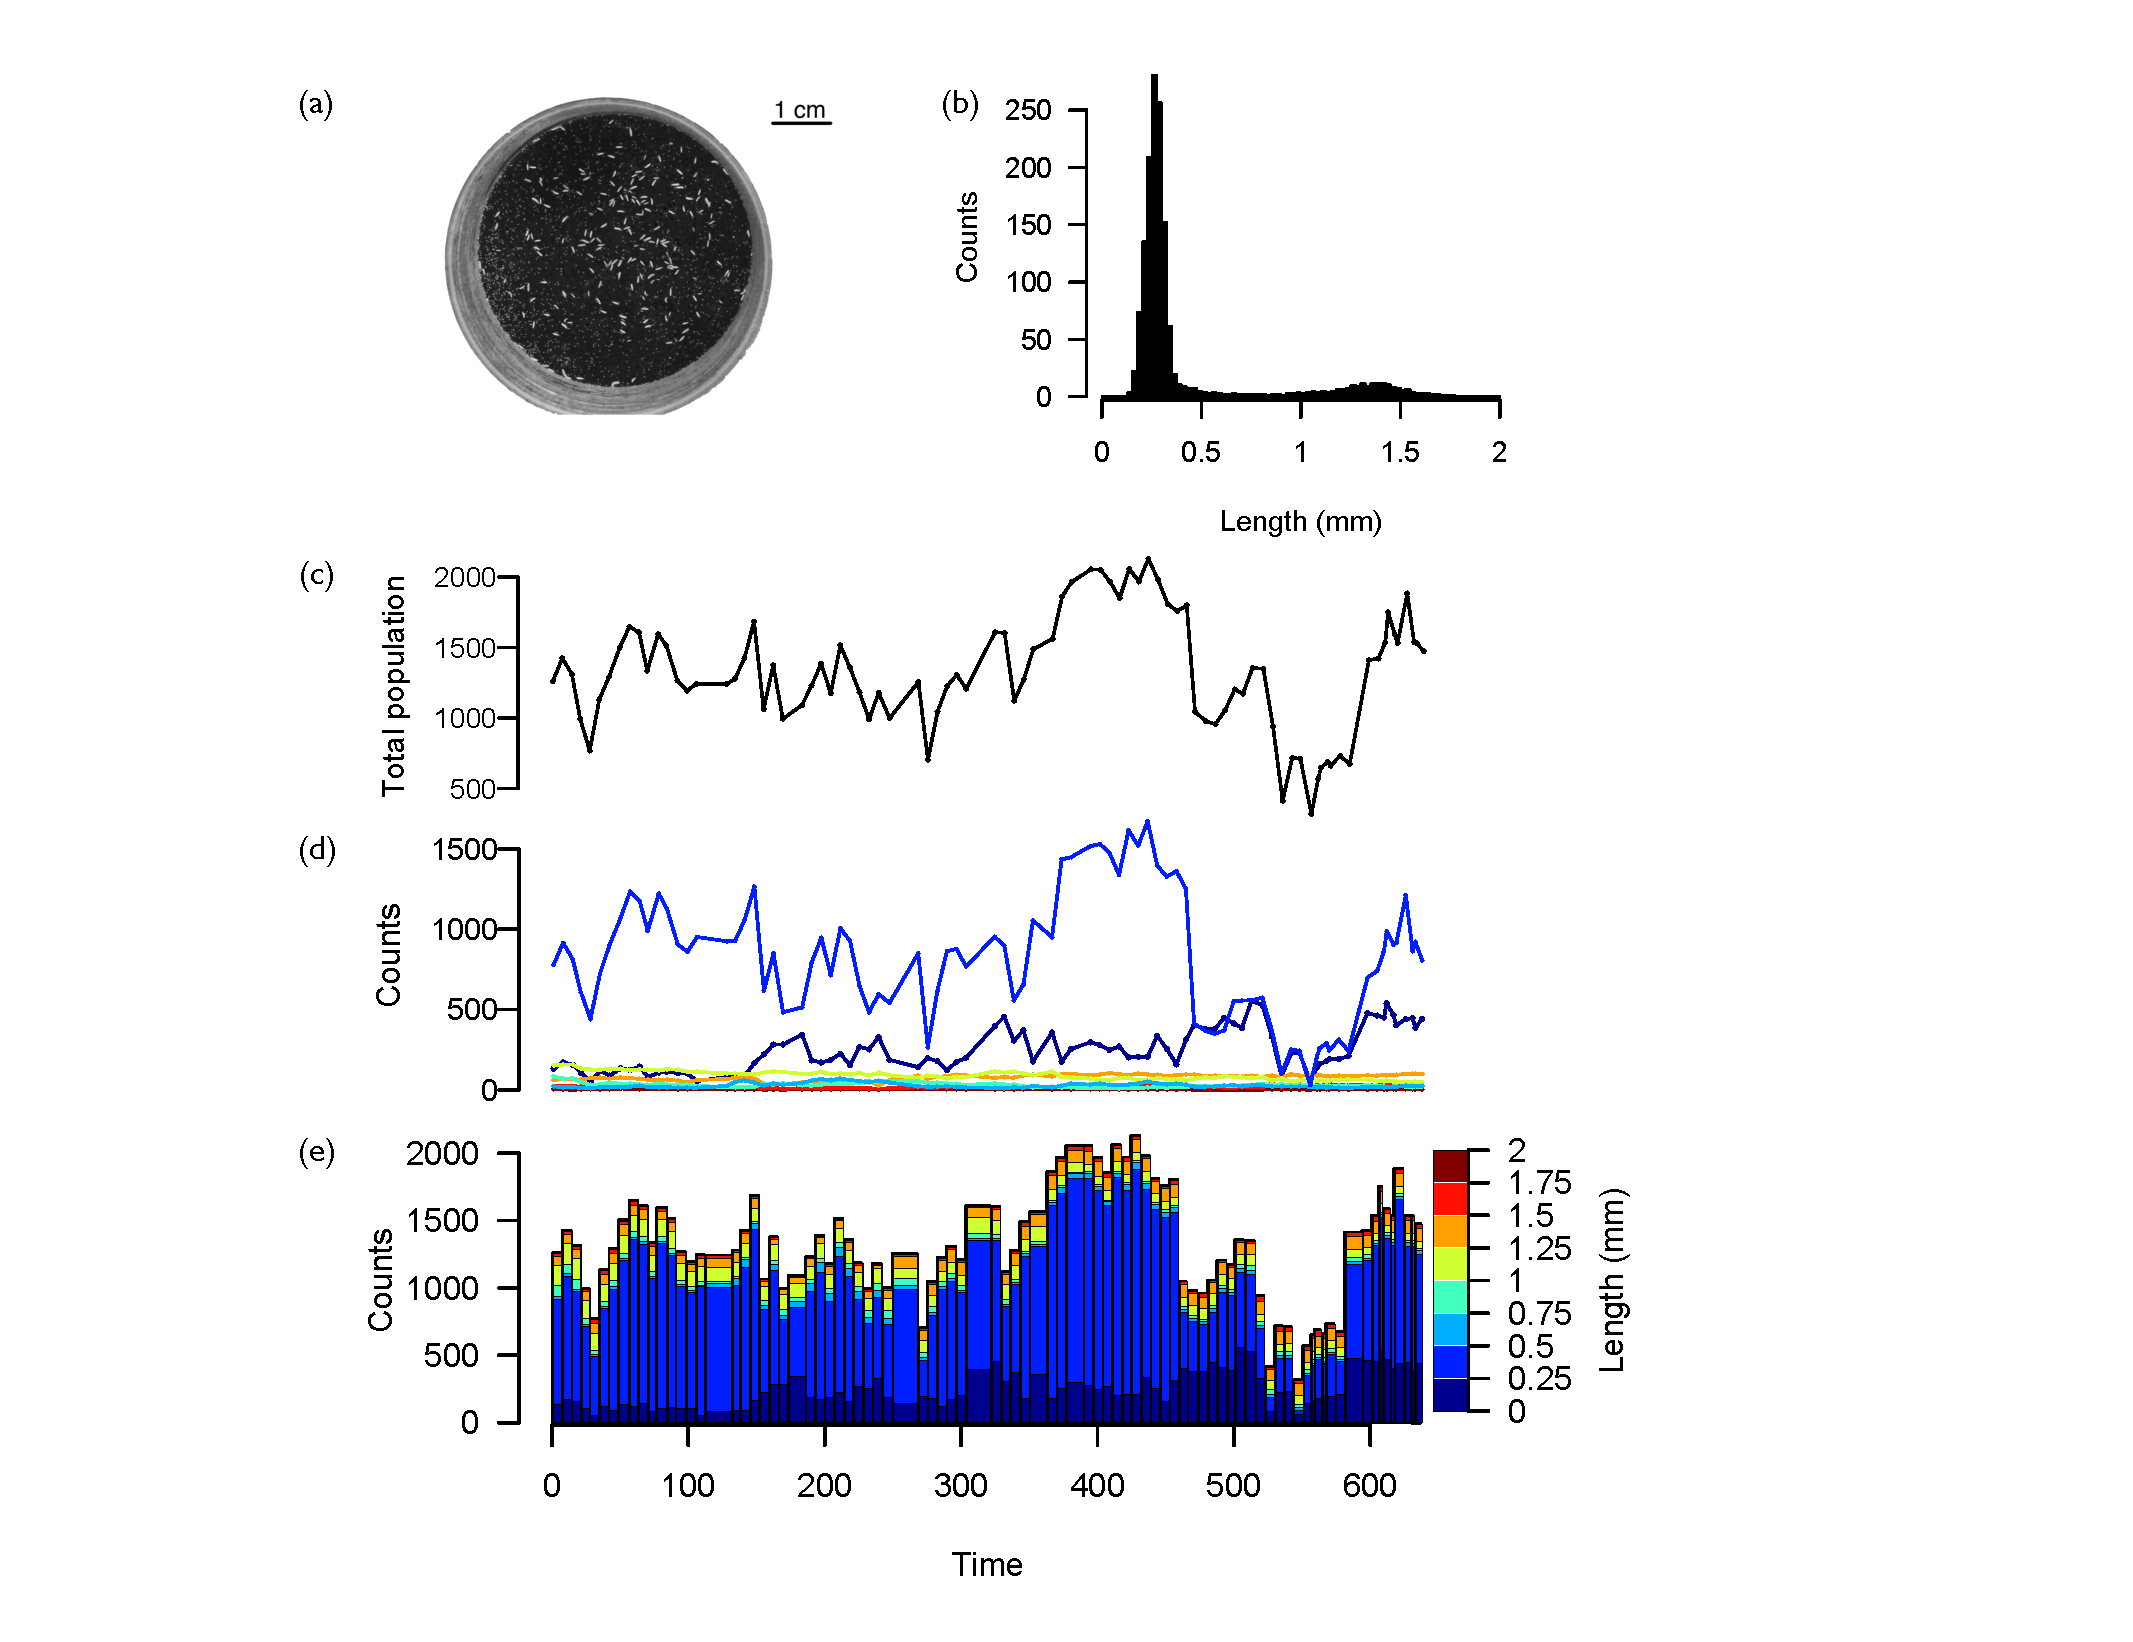
\includegraphics[height=0.75\textheight]{2_Methodo/Fig/Fig22-1.pdf}
\caption[\lofimage{2_Methodo/Fig/Fig22-1.pdf}Classical representation of a
population structure]{ We used as a practical example an experimental population
of the Collembola \textit{Folsomia candida} (a) whose structure has been measured every one or two weeks . The size structure at one time is classically shown as a histogram (b) and the total population dynamics on a time series plot (c). To represent both the structure and temporal dynamics, the population has been divided in
several size classes to plot their dynamics independently (d) or to produce a
stacked bar plot (e). While these representations underline the dynamics inside
each size classes, the patterns of dynamics between adjacent classes remain
hidden.great confidence.
}
\label{Fig22-1}
\end{figure}


We made the R-package \texttt{STdiag} to provide a user-friendly interface for
representing time series of structured populations using heatmaps. We detail how
to generate such graphics and discuss their biological interests using (1) the
long-term structure dynamics of experimental laboratory populations of the
Collembola \textit{Folsomia candida} (Figure \ref{Fig22-2}), (2) a long term study of a population of
common lizards Zootoca vivipara in France (Figure \ref{Fig22-3}) and (3) an example in the
field of pharmaco-epidemiology: the seasonal dynamics of the annual consumption
of antibiotics in France (Figure \ref{Fig22-4}).

\section{Method overview}

The diagram produced by \texttt{STdiag} shows a structuring element (age, size,...) along
the $Y$-axis and time along the $X$-axis. These variables are usually continuous
but have to be made discrete and then put into several classes, the number and width
of which depend on the quality and size of the available dataset. For each time
and structure class coordinate, a colour rectangle is plotted whose hue refers
to the number of individuals (or any other statistics such as frequency or rate)
in that class (possibly on a logarithmic scale) at the given time. This
representation puts side-by-side colour histograms for each time value and
emphasises the temporal dynamics according to the structure of the population.

\section{Package STdiag usage}

To easily display the dynamics of a structured population we made the package
\texttt{STdiag} which is freely available at R-forge (\url{R-forge.r-project.org/}) and
can be installed in R with the following command:

\begin{verbatim}
install.packages('STdiag',repos="http://r-forge.r-project.org")
\end{verbatim}

\subsection{Importaing and formating the data}

\subsubsection{Data frame.}
\texttt{STdiag} uses the lattice function \texttt{levelplot}
\autocite{sarkar2008a}.
As a consequence, the basic data format is a three column data frame containing the
$X$ (time), $Y$ (structure such as age or size) and $Z$ (number of individuals)
coordinates. The data frame has $TxS$ lines where $T$ is the number of time
values and $S$ the number of structure classes.

\subsubsection{Matrix.}
Another possibility is to use a matrix description of the data using two vectors
$x$ and $y$ of size respectively $T$ and $S$ for the time and structure
coordinates, and a matrix $z$ of size $TxS$ containing the number of individuals
at each coordinate. This mimics the format used by function image \autocite{team2012a}.
In case one wishes to use the frame format for data in the matrix format, the
function \texttt{Matrix2DataFrame} is provided:
\begin{verbatim}
DataFrame <- Matrix2DataFrame(z, x, y, xlab="time", ylab="structure",
zlab="number").
\end{verbatim}

\subsubsection{Individual based data.}
The function \texttt{Indiv2DataFrame} is also provided to convert
individually based data to a data-frame that can be plotted with \texttt{STdiag}. This function handles a
data-frame containing one line per individual and, for each individual, the time
of the observation in the first column and the value of the structure in the
second one. The option classes, allows to control the number of classes to
discretize the structure variable. A single value produces the wanted number of
regular classes (default set to $50$), whereas a vector specifies the breaks of
the classes as in function hist. This function is used as follows:
\begin{verbatim}
DataFrame <- Indiv2DataFrame(IndivData, classes=50).
\end{verbatim}

\subsection{Generating the plots}

\subsubsection{Data frame.}
The simplest way to generate the basic plot is to use the data frame
formulation. If the columns of the data frame are in a time-structure-number
order, a simple call to
\begin{verbatim}
STdiag(DataFrame)
\end{verbatim}
will produce the plot. If one wants to specify what column to plot, the function
\texttt{STdiag} accepts the formula syntax:
\begin{verbatim}
STdiag(number ~ time * structure, data= DataFrame).
\end{verbatim}
In any of those or the following forms, the vector used as time can either be a
numeric vector or a vector of dates of classes \texttt{POSIXlt},
\texttt{POSIXct} or \texttt{Date}. Class \texttt{factor} is not yet supported
for date format.

\subsubsection{Matrix.}
To use the matrix formulation, call either
\begin{verbatim}
STdiag(Matrix)
\end{verbatim}
in which case $X$ and $Y$-axes will be default vectors from $1$ to respectively
$T$ and $S$. Or, if one wants to specify the $x$ and $y$ coordinates,
\begin{verbatim}
STdiag(x=time, y=structure, z=Matrix).
\end{verbatim}

\subsection{Improving the graphical representation}

Our method is implemented with several options to adjust the plot to be as
informative as possible.

\begin{figure}[!ht] % Figure 2 
\centering
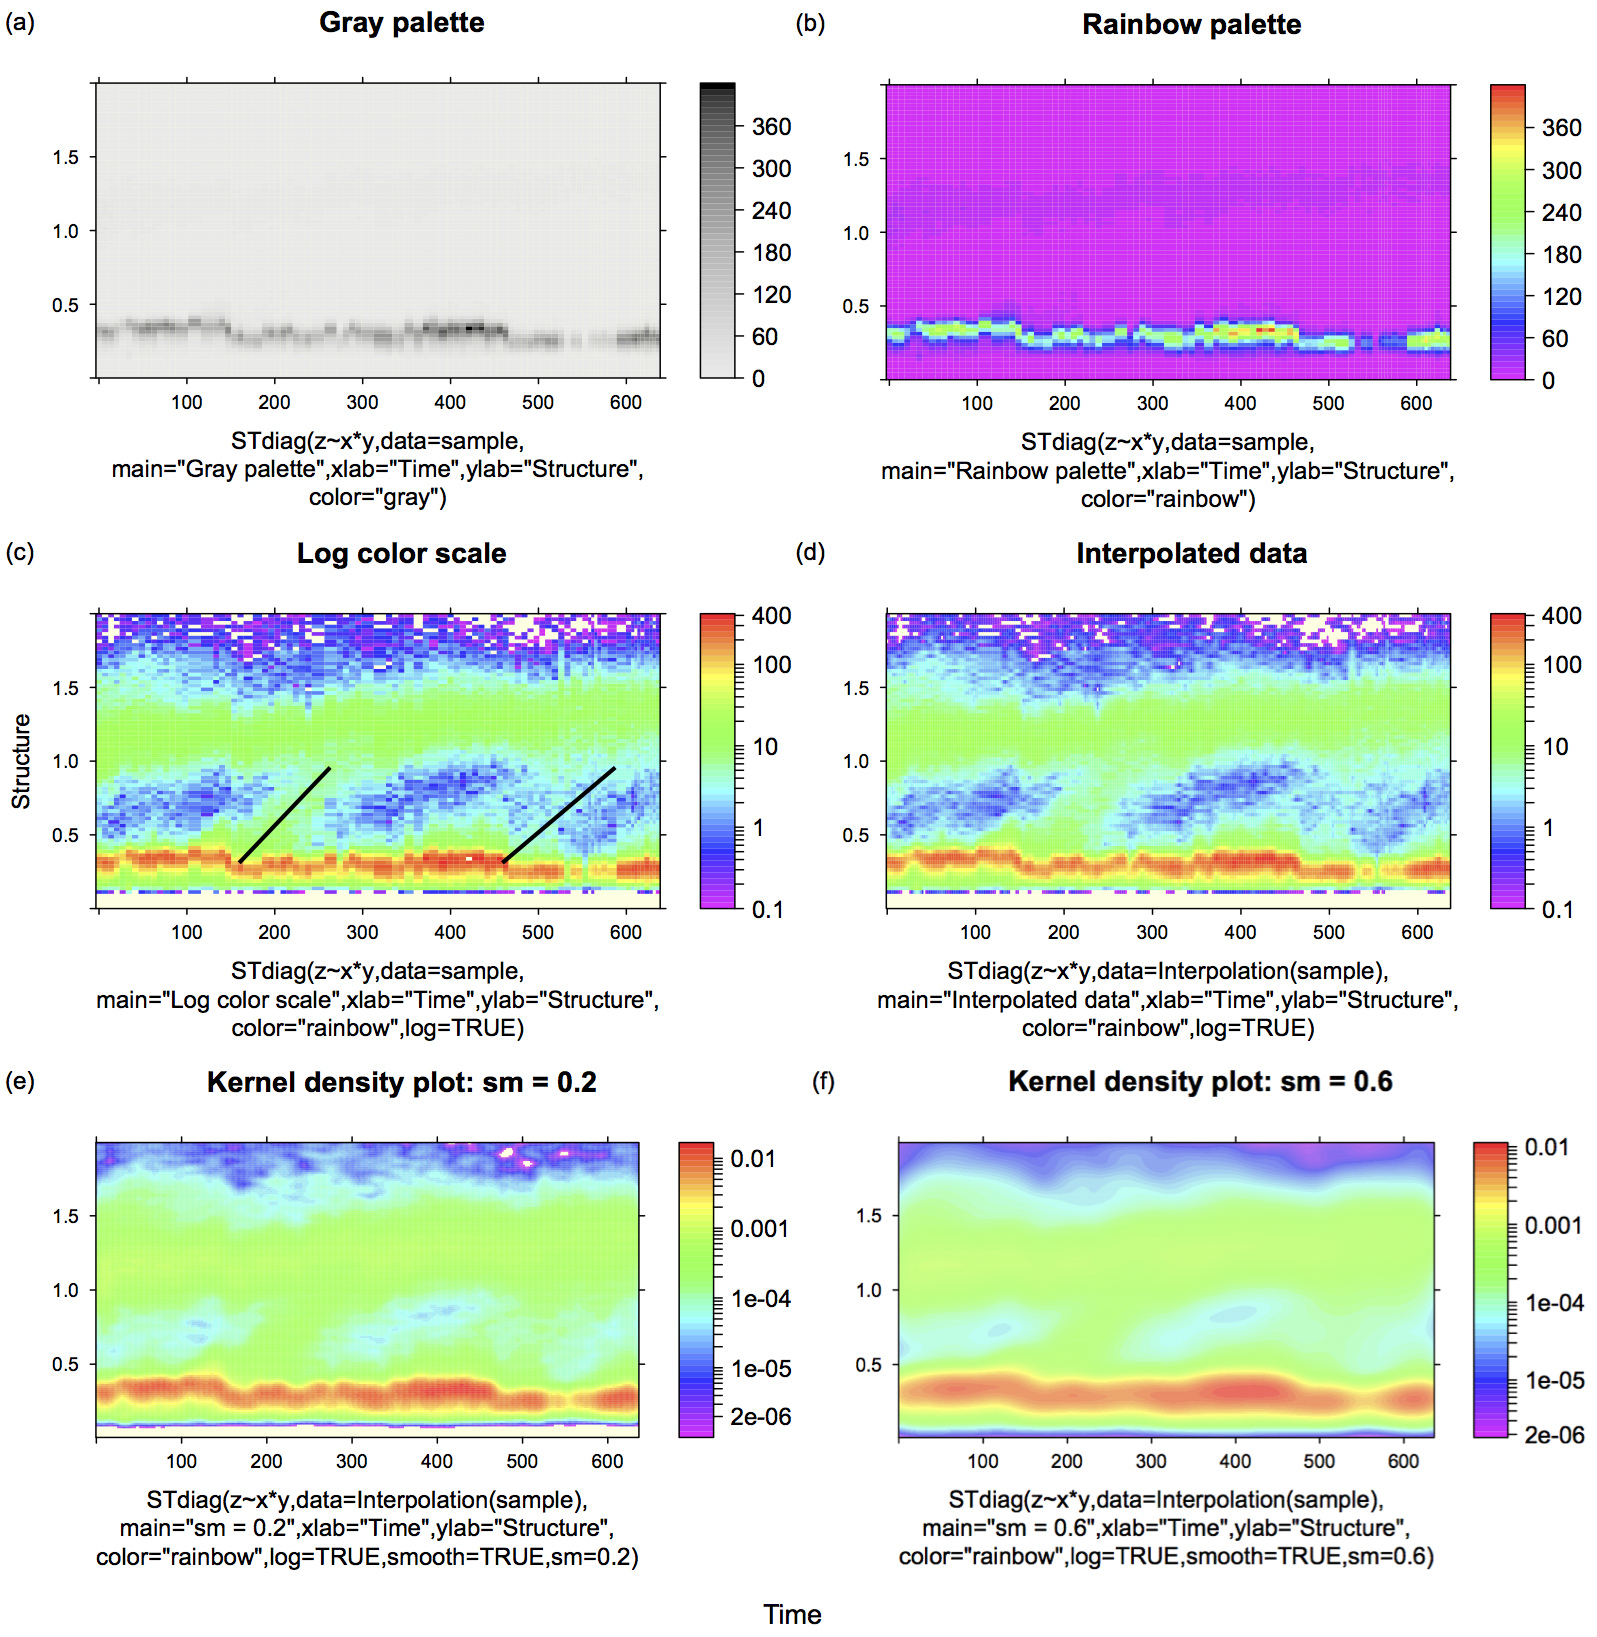
\includegraphics[height=0.70\textheight]{2_Methodo/Fig/Fig22-2}
\caption[\lofimage{2_Methodo/Fig/Fig22-2}Collembolan population dynamics plotted
with STdiag]{ Collembolan population dynamics plotted with STdiag. The code to produce each plot is given in each panel. Length is discretised into classes of
0.05mm length. Number of individual at each date length coordinate is
represented on a linear grey (a) or colour (b) scale or on a logarithmic scale
(c, d). Panel (d) represents an interpolated version of panel (c). Panels (e)
and (f) represent two kernel density estimates with increasing smoothness. The
population is mostly composed of small individuals ($\approx0.4$ mm) living with some
adults ($\approx1.2$ mm). Logarithmic scale reveals details about the recruitment of
some cohorts, the growth rate of which can be estimated (black lines, c).
}
\label{Fig22-2}
\end{figure}

\subsubsection{Colour palette.}
The readability of the diagram partly relies on the choice of colours for the
palette (Figure \ref{Fig22-2}a, b). The hues are sorted following either a gray scale from
pale gray to black or a rainbow gradient (Figure \ref{Fig22-2}a, b, c).This can be adjusted
using the option color="palette" inside \texttt{STdiag()} where palette can be
one of the following: \texttt{gray, topo, terrain, heat, cm, rainbow} or by
default \texttt{tim} (see tim.colors in library fields, \citealp{furrer2012a}).

\subsubsection{Logarithmic scale.}
When the number of individuals in the different classes differs by several
orders of magnitude (Figure \ref{Fig22-1}b) we recommend using a logarithmic scale to increase
the readability of the generated graphics. The option
\texttt{log=TRUE}$/$\texttt{FALSE} allows the user to switch easily between
linear and logarithmic colour scales.

\subsubsection{Interpolation.}
The quality of the diagram can sometimes be improved by applying an
interpolation to smooth the representation and link together uneven time
intervals by creating evenly spaced data (Figure \ref{Fig22-2}d).The interpolation method
create an artificial dataset with evenly distributed data, based on the original
data. It is essential to make a clear distinction when reading such a diagram
between the real data and data created by the interpolation and we recommend to
first use a non-interpolated representation of the data. To interpolate the
data, we provide in the package the function Interpolation. This function is an
interface to function interp.surface in package fields adapted to quickly handle
data accepted by function \texttt{STdiag}. It takes as argument the data frame
to be interpolated in the form of three columns: time, structure and number of
individuals, in that order. The options \texttt{intervX} and \texttt{intervY} allow the user to
manually choose the intervals between two interpolated points, respectively over
$X$ (time) and $Y$ (structure) axes. If those options are left empty, the
function uses the minimum distance between two points in the first and second columns as
intervals for respectively $X$ and $Y$ axes.

\subsubsection{Kernel density estimate.}
The function STdiag~provides an option \texttt{smooth=TRUE}$/$\texttt{FALSE} to
plot a weighted kernel density estimate of the data using an axis-aligned bivariate normal
kernel, where the data are the time-structure coordinates weighted by the number
of individuals. The estimate is derived from the function \texttt{kde2d} in
package \texttt{MASS} \autocite{venables2002a}. The density estimate can be
adjusted with options sm, a positive scalar ($0$ meaning the original data and $1$ being
the normal reference distribution kernel estimation bandwidth) defining the smoothness of
the kernel density estimate, and $n$, the number of points on the $X$ $Y$ grid.
Together, these options allow to view a smooth representation of the structured
data (Figure \ref{Fig22-2}e, f, Figure \ref{Fig22-3}). Contrary to the interpoation, the kernel density
estimate only provides a smooth representation of the data. In the case of
missing data, such as irregular time intervals, interpolating the data before
plotting the kernel density can avoid having gaps in the density for a low
smoothing factor (small \texttt{sm}).

\section{Reading and interpreting ST diagrams}

\subsection{Dynamics of a laboratory population of collembolan.}
We used as a first practical example of temporal dynamic of a structured
population, some data issued from the close follow-up of an experimental
population of a springtails maintained in our lab during about $600$ days. We
studied the species \textit{Folsomia candida} that is commonly used in laboratory and is
easy to breed and maintained \autocite{fountain2005a}. This is
an ametabolous parthenogenetic hexapod whose populations are composed only of females of
different size because the juveniles look like minute adults and the adults
continue to mould and grow after reaching maturity. The individuals were bred at
$21 \degres$C in cylindric plastic boxes of $5.3$ cm diameter with a $3$ cm thick
plaster substrate to keep the environment damp \autocite{tully2008a} (Figure
\ref{Fig22-1}a). The population is fed weekly with a mix of yeast in agar-agar in a fixed quantity
and kept in the dark the whole time. Measures of the number and size of
individuals are taken every one or two weeks using picture analysis with the
image processor ImageJ \autocite{abramoff2004a,mallard2012a,mallard2013a}
providing the structure of the population at each time of measure (Figure \ref{Fig22-1}b).

The structured time diagram (Figure \ref{Fig22-2}) immediately reveals the predominance of the
younger class ($<.5$ mm). The use of a log scale (Figure \ref{Fig22-2}c),
reveals some inter-class dynamics undetectable using classical representations: between day
$150$ and day $300$ a cohort of small individuals grows and recruits into the
adults. This visual display allows one to estimate some demographic parameters
that cannot be read on classical representations (Figure \ref{Fig22-1}): size at
birth ($\approx0.28$ mm, by observing spikes of births), adult length ($1.9$ mm around
day $50$), growth rate of a cohort of juveniles fighting to be recruited in the
population ($0.22$ mm.month$^{-1}$, slope of the straight line of Figure
\ref{Fig22-2}c).

\subsection{Dynamics of a wild population of common lizards.}

As a second study example we used individual-based mark-recapture data collected
from 1989 to 2004 in a population of common lizards from the Mont Lozère in
southern France ($1420$ m a.s.l, $44\degres30$’N, $3\degres45$’E). Data collection
each year was structured as follows: a capture session of yearlings ($1$ year
old individuals) and adults in June-July and a temporary transfer of pregnant females to the
laboratory to mark and measure juveniles from birth \autocite{le-galliard2010a}.
The Figure \ref{Fig22-3} reports the size structure (snout-vent length) of the
population. We used a total of $7486$ measurements, $3935$ females and $3551$
males.

The Figure \ref{Fig22-3} clearly shows the long term dynamic of the population structure:
males are on average smaller and less captured than females. Compared to other
exemples, the dynamic of the population structure is relatively discontinuous
(Figure \ref{Fig22-3}). The population structure is multimodal along the size axis because of
the annual reproduction, and is discontinuous along the time axis because the
sampling was not perfomed during the six months of the hibernation period. The
sampled population is composed of newborns ($\approx2$ cm), yearlings ($\approx4$ cm) and
adults ($>5$ cm). The figure also shows at a glance some secular changes in the
mean size of both adults and yearlings: the body length in the population increases from
1989 to 1994 \autocite{chamaille-jammes2006a} and decreases
thereafter.

\begin{figure}[!ht] % Figure 3 
\centering
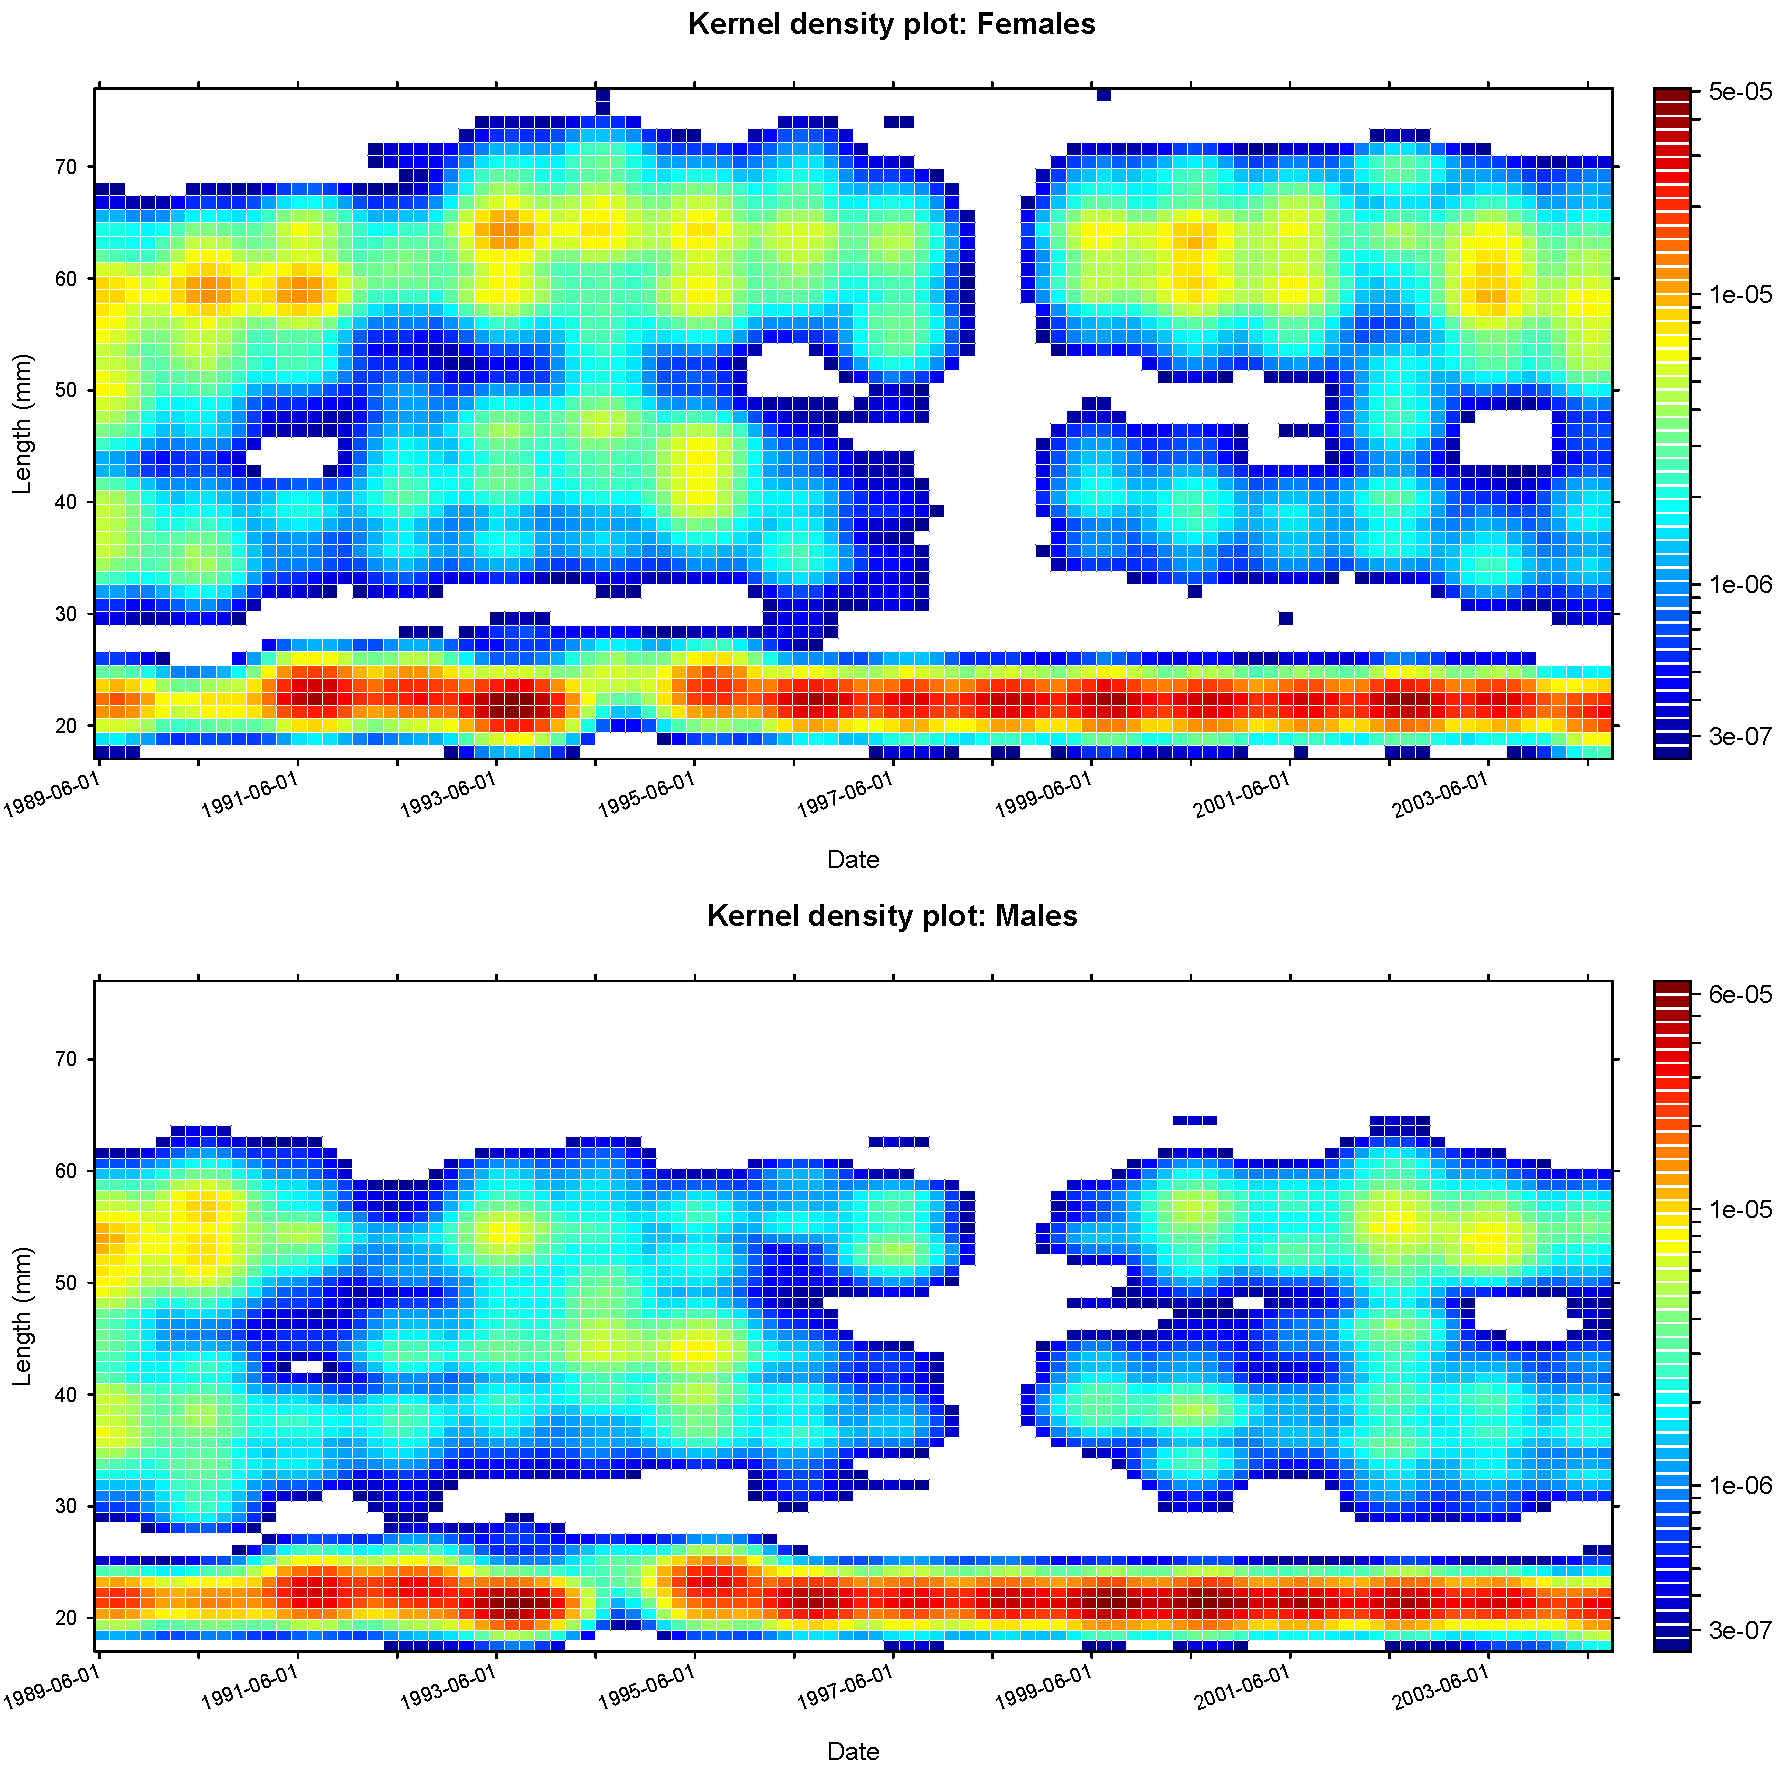
\includegraphics[width=0.85\textwidth]{2_Methodo/Fig/Fig22-3.pdf}
\caption[\lofimage{2_Methodo/Fig/Fig22-3.pdf}The follow-up of a population of the common lizard]{ The follow-up of a population of the common lizard. The plots represent the
population size structure (snout-vent length) of the animals (females, first
row, and males second row) captured in the population each spring. Capture
pregnant females are kept in the laboratory until parturition and the juveniles
are measured right after birth. In 1998, for exceptional reasons the prospection
effort was very low and very few adults of sub-adults have been captured and
measured. The population structure and the long term changes of snout-vent
length can be easily seen on these graphs. We used here a log scale and a kernel
density plot. The large "dots" that are apparent with regular frequency on the
Female plot result from the seasonal annual census of the population.
}
\label{Fig22-3}
\end{figure}


\subsection{Antibiotics consumption}

Our last example -- the consumption of antibiotics in France -- is an
application of our method in the field of pharmaco-epidemiology. It illustrates the
powerfulness of this graphical display to make database of tens of millions of
observations almost instantaneously understandable. We have used data from the
French national database provided by the CNAMTS (“Caisse nationale d’assurance
maladie des travailleurs salariés”, national fund of health insurance for
employees), which covers $75\%$ of the French population. In this specific
example, one can easily see that the purchase of antibiotics decreases every
weekend and during public holiday because most of the chemist shops are closed
(vertical bars on Figure \ref{Fig22-4}a). One can see also that on average, more antibiotics
are purchased for children than for adults. But more interestingly, the plot
reveals the seasonal change in antibiotic consumption for each age class in the
population (Figure \ref{Fig22-4}a):  the seasonal variation in children antibiotic consumption
follows the periods of holidays while for adults and elderly people, the plot
(Figure \ref{Fig22-4}a) specifically underlines the detailed topology of the burden of
purchases that has arisen during the H1N1 influenza pandemic which occurred from
September 2009 to January 2010 in France (Figure \ref{Fig22-4}b, c;
\citealp{lemaitre2010a,lemaitre2012a}).

\begin{figure}[!ht] % Figure 4 
\centering
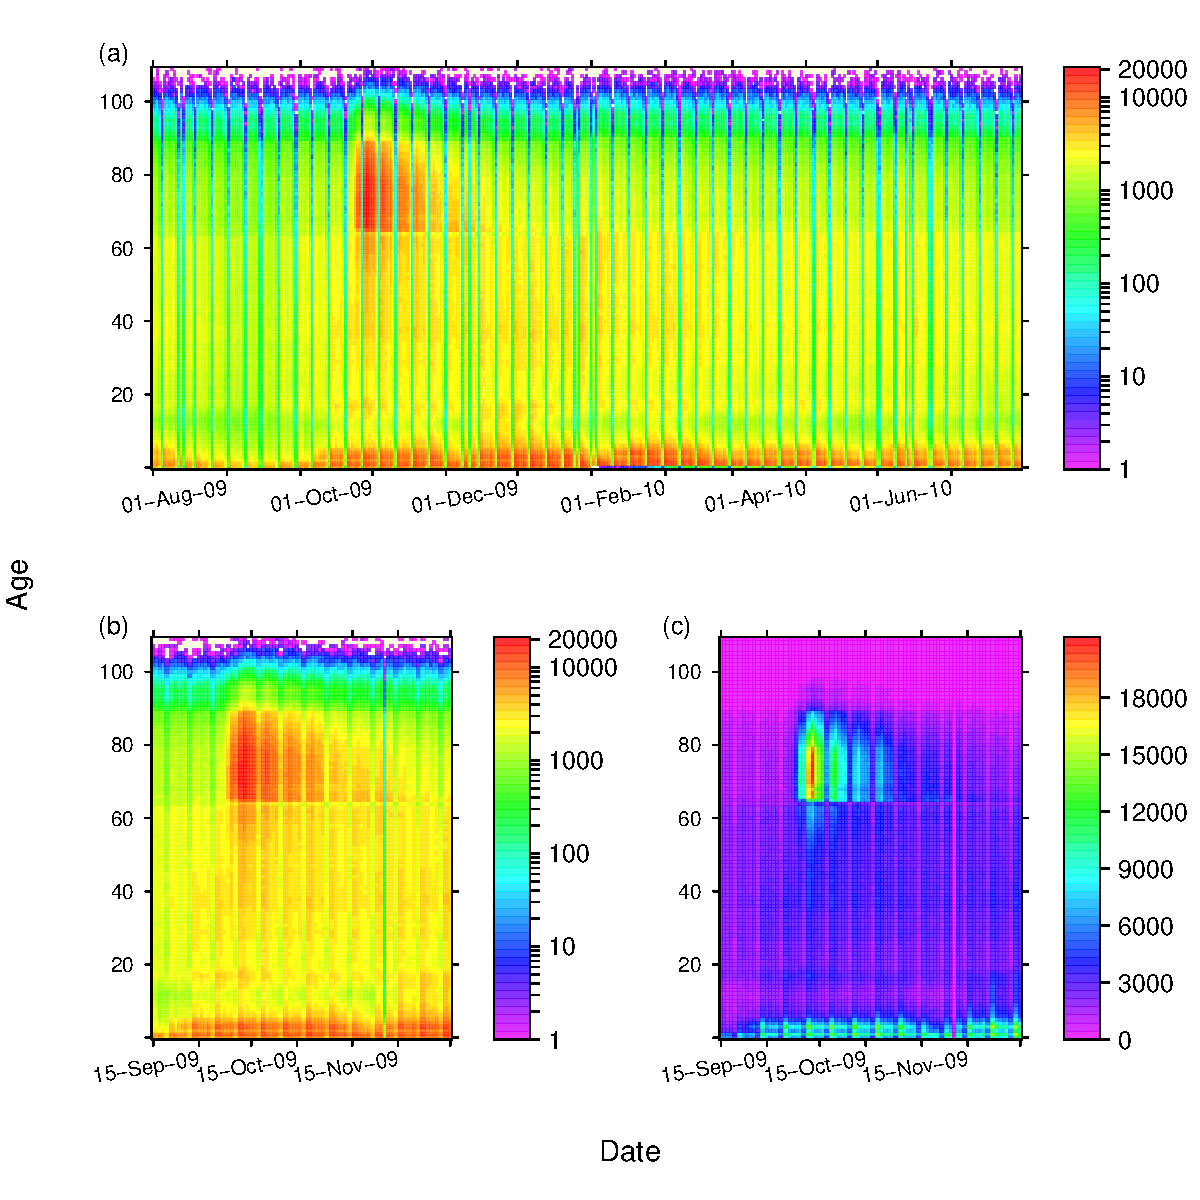
\includegraphics[width=0.85\textwidth]{2_Methodo/Fig/Fig22-4.pdf}
\caption[\lofimage{2_Methodo/Fig/Fig22-4.pdf}Antibiotic consumption in France]{ Graphical representation of the antibiotic consumption in France from 1st July
2009 to 30th June 2010. The number of antibiotics bought in chemist’s shop is
shown for each age class (68 millions of observations). (a) The full
representation reveals the structure by week (the purchases of antibiotic falls
off during the weekend and public holiday), the seasonal fluctuations (less
consumption during spring and summer seasons) and a wave of consumption in
autumn 2009. The vacations give rhythm to the children’s antibiotic consumption.
Removing saturday and sunday allows a cleaner view of the data, and a close-up
view on the autumnal wave of purchases on a logarithmic (b) or linear (c) scale
reveals the increase in antibiotics consumption following the outburst of H1N1
during that period.
}
\label{Fig22-4}
\end{figure}


\section{Conclusion}

A multi-dimensional diagram such as our structure--time diagram (Figure \ref{Fig22-2}b) is
preferred to a simple time series representation (Figure \ref{Fig22-1}c, d) for several
reasons: time series representation lacks the continuity of the structuring
element. Although time series plots and time series analyses are very powerful
and bring useful information on dynamics inside classes that are artificially
created, such as number of individuals or existence or not of a periodicity, the
small number of classes usually used and the representation in lines make it
very difficult to read and therefore detect and analyse any cross classes
dynamics. A three-dimensional diagram offers a unique and complete visual
display of the variations of the population structure and is thus a very
powerful tool for the description of a population and a convenient way of
guiding the analysis. Moreover, by juxtaposing several structure--time diagrams
one can add an extra dimension to the graphical display, such as the sex of the
individuals as in the lizard example (Figure \ref{Fig22-3}) or any other categorical variable
(population, genotype etc.). If one uses the same axis for these diagrams, one
can in a glance compare the complex dynamics of several categories of
individuals.

The structure--time diagram does not need individuals to be identified from one
time to the other. And without any individual trajectories, changes in the
structure over time directly draw dynamics of cohorts (as in Figure \ref{Fig22-2}c).

STdiag can also be used to represent any type of data with a structuring factor
and an aggregate statistic. For instance, this method can be used to represent
the average mortality rate in each age-time class \autocite{vaupel1987a}, or the evolution over time of the average size depending on the age,
illustrating the shrinkage of Soay sheeps \autocite{ozgul2009a}. It
can also be used for displaying data from a population model such as a physiologically
structured one \autocite{metz1986a}. It can also be applied to
follow the temporal dynamic of a human population structure coming for instance from
medical survey to detect any secular or seasonal changes for example (Figure \ref{Fig22-4}).

Such diagrams fulfil the criteria for excellence in statistical graphics
\autocite{tufte1990a}: they show many numbers within a small space (high
data density) thus making coherent large data sets without distorting the data; they reveal the
data at several levels of detail, from fine structure to broad overview,
encourage the eyes to compare different pieces of data and induce the viewer to
think about the substance rather than about the method \autocite{tufte2001a}.

With the development of automatic data acquisition and prolific databases
\autocite{le-galliard2012a,mallard2012a,mallard2013a}, the use of such a
graphical display should become more common in population ecology but also in many other fields such as epidemiology or medical
surveys.

\section{Acknowledgments}

We thank the Programme interdisciplinaire du vivant Longévité et vieillissement
funded by the Centre National de la Recherche Scientifique (CNRS) and the French
Research National Agency (ANR EvoRange), reference ANR-09-PEXT-011 for
supporting this project.

We thank Guillaume Sapriel, Jean-Louis Galliard and Didier Guillemot for helping
us applying this method in the field of pharmaco-epidemiology and we are
grateful to the French Health National Insurance (CNAMTS) for providing the
antibiotic data used to construct Figure \ref{Fig22-4}.

%\part{Compétition par interférence et populations structurées}

\chapter{Interference competition and size dependent resource
access mediate size structure dynamics. Experimental approach using laboratory
populations of Collembola \textit{Folsomia candida}}\label{Ann:SP}
\chaptermark{Interference competition in experimental populations}

\vspace{2cm}

\begin{Spacing}{1}
\texttt{
Le Bourlot, Vincent, François Mallard, Monique Avnaim, Romain Peronnet, David
Claessen and Thomas Tully, "Interference competition and size dependent resource
access mediate size structure dynamics. Experimental approach using laboratory
populations of Collembola \textit{Folsomia candida}"\\
Manuscrit en cours d'écriture pour soumission à Journal of Animal Ecology}
Voir Chapitre \ref{chap:sp}.
\end{Spacing}


\section{Introduction}

Understanding the functioning of ecosystems and the response of species to their
environment requires the comprehension of their demography and population
dynamics. A common finding from studies of empirical and natural populations
(from laboratory experiments like Drosophilia  or soil mite, to populations in
the field such as Soay sheep  or red deer) is that populations are generally
structured in non-trivial ways.
This means that describing a population as a group of obvious stage classes such
as juveniles and adults often does not encompass enough complexity to reflect
the actual mechanisms at play in the interactions between individuals and with their
environment, governing the population dynamics.

In a population, the structure comes from the individual heterogeneity.
The biggest cause of heterogeneity is due to the individual life cycles and the
different stages in the cycles that individuals occupy. Accounting for
the population structure is important for several related reasons, and
especially because (i) one completion in the life cycle takes a finite time to
complete, and (ii) being in different stages in the cycle will lead to different
environmental impacts on and by the individual, (iii) eventually leading to the
population structure affecting its own dynamics. For instance, Benton and
Beckerman (2005) have shown that in the same controlled environment, several
populations with different initial structure but similar density would lead to
diverging trajectories at the level of the population. More precisely in this
case, adults would respond to food availability by increasing fecundity whereas
juveniles would favour individual growth. It is this difference in the
individual impact and response to the environment that leads to the differences
in population dynamics. Even when the model species is chosen for its apparent
simplicity, such as rotifers \autocites{fussmann2005ecological}, it has
been shown that it is necessary to account for age structure to be able to
correctly describe the empirical results in a mathematical model.

Population structure also influences the population dynamics because of
the delay imposed by the completion of the life cycle. Not only do
different stages respond differently to the environment, but the time lags
generated by the life cycles tend to destabilize the dynamics. Models of
physiologically structured populations have shown that the juvenile delay – the
time for a newborn to reach maturity and start reproducing – along with
differences in competitive ability between different sizes can lead to unstable
population dynamics that oscillate with a one generation period. On the
contrary, a more even competition between the different stages generally tends to
stabilize the population dynamics.

Among the individual interactions that are directly affected by the population
size structure – that we will refer to as “population state” – is the
competition to access available resources. Competition is defined as an
interaction between organisms such that one’s performances are reduced by the
presence of others
\autocites{volterra1931a,gause1932a,park1948a,park1954a,park1957a}.
Competition can either be exploitative (scramble) or by interference (contest)
\autocites{park1954a,park1962a,begon2009a}. Exploitative competition is indirect
and mediated by the resource
\autocites{goss-custard1980a,vance1984a,begon2009a}, and causes a decrease in
the individuals’ intake rate because other individuals are depleting the
resource. It does not require any physical interaction but requires for the
resource to be limiting \autocites{begon2009a}.

On the contrary, interference competition is a direct competitive interaction
between individuals. It happens when one individual reduces the other’s ability
to exploit a common resource through negative direct interactions, regardless of
its abundance \autocites{park1954a,vance1984a}. These interactions can be
aggressive displays\autocites{schoener1976a}, territoriality
\autocites{walls1990a,kennedy1996a}, allelopathy
\autocites{harper1977a,rice1984a,nilsson1994a}, overgrowth
\autocites{connell1961a,paine1966a}, \textit{etc}. One of interference
competition's main mechanisms is for a superior individual to deny resource
access to the inferior one \autocites{schoener1983a,thompson1993a}. To be
competitively superior one often needs a superior physical strength, which is
generally related to a superior body size \autocites{mccormick2012a}.
When considering intraspecific competition in a single population, accounting
for the population state is then mandatory to properly understand the regulation
mechanisms at play.

To date, the consequences of interference competition on size structured
populations remain poorly explored. We used the Collembola \textit{Folsomia
candida} to investigate how a population state influences its dynamics and
future structure.
Folsomia candida is a convenient species for studying population dynamics, life
history trajectories and phenotypic plasticity
\autocites{tully2005a,tully2008a}.
It is an easy to breed parthenogenetic species \autocites{fountain2005a} that
allows for detailed population survey with individual body length and population
state measures.
Bred in small rearing boxes with weekly resource input \autocites{tully2008a} we
started 28 populations of two different clonal lineages with different initial
conditions, and censused each population weekly for 800 to 1200
days. We then performed both a qualitative and quantitative analyses of detailed
time series of each population’s size structure to determine the relationships
between the past and present state with the future structure dynamics, and
especially understand the role of larger individuals in its regulation.

\section{Methods}

\subsection{Model organism}

In our study, we use the Collembola \textit{F. candida} as a model
species.
\textit{F.
candida} is a blind ametabolous hexapod widely distributed around the globe. It
usually lives in humid habitats such as decaying litter, rotting wood or caves
\autocites{fountain2005a}. With a length up to few millimeters for the biggest
individuals, it is easy to breed in the laboratory in controlled microcosms with
finely controlled abiotic (temperature, humidity, light) and biotic (resources)
conditions. Every stages of the life cycle (egg, nymph and adult) are visible
and share the same environment and resources (after hatching), allowing for
measurements and manipulation throughout their life. Growth occurs by molting
during the whole life span every 10 to 20 days.

We use two different genetic lineages that we label respectively "HA" and "TO".
Both lineages are parthenogenetic. They are kept in separate populations so that
in each of our populations, every individuals share the same genotype. Each of
these lineages are known for their highly flexible phenotypic adjustment when
facing sudden environmental changes, in density, temperature, resource
abundance, \textit{etc} \autocites{tully2008a,mallard2013b}.

\subsection{Rearing conditions}

16 populations of clone HA and 12 populations of clone TO are kept in standard
rearing boxes made of polyethylene vials, with a 52 mm diameter and a 65 mm
height. The boxes are filled with a 30 mm layer of plaster of Paris stained in
black with Pébéo Graphic\circledR Chinese ink to ensure sufficient contrast between the
dark background and the light Collembola for easy numbering and measurements
\autocites{tully2008a,mallard2013a}.

Populations are bred at $21\degres$C in the dark in closed incubators (FOC 225E,
temperature controlled $\pm 0.5\degres$C). The plaster is moisturized regularly
to keep the humidity at saturation in the rearing boxes. Resource is provided once a week
under the form of small pellets of a mixture of dried yeast and agar in
standardized concentration and volume (5000 mL water+80 mg agar+800 mg dried
yeast, to produce $15 \mu$L pellets).

\subsection{Long term population surveys}

Populations of both HA and TO clonal lineages are monitored during 800 to
1200 days ($90$ to $170$ points). Populations are initialized with a random
number of juveniles and adults. Each population is numbered and individuals are measured
weekly using a dedicated plugin for the image analysis software ImageJ
\autocites{abramoff2004a,mallard2012a,mallard2013a}
(\url{http://rsbweb.nih.gov/ij/}).
At each date of measure, we obtain the number of individuals in the population together with
individual measurements of the body length. These measurements allow use to
access the population's size structure and some individual's life history
traits, such adult asymptotic length or juvenile growth rates in population
conditions.

\subsection{Qualitative analysis of population structure and dynamics}

We looked at the long-term size structure dynamics using a three dimensional
graphical representation that we refer to as a "structure-time diagram". A
structure-time diagram shows the time in abscissa and the body length in
ordinates. We then represent the size-structure of a population at a given time
by measuring the distribution of the individual’s body length at that time and
representing it by creating a histogram and coding the log-frequency in each
size-classes on a color gradient. This produces a column of colored pixels that
represent the distribution of the body length in the population. By repeating
this method for each date, using the same color gradient, and juxtaposing them
on the time abscissa, this produces a colored representation of the population
size structure dynamics over time with a high density of information on a
relatively low-space consuming figure. Such a diagram can easily be produced
using the "STdiag" package available on R-forge
(\url{https://r-forge.r-project.org/projects/stdiag/}). Structure-time diagrams
for every population studied are available in the supplementary materials.

\subsubsection{Population state}

We look first at the global population’s size structure. Using structure-time
diagrams, for each population we observe the complete time series and try to
define periods of time corresponding to stable size structures without
considering the short-term dynamics. We describe several population states
depending on the clonal lineages and the conditions of density.

\subsubsection{Population size structure dynamics}

On the same structure-time diagrams, we then look at the different short-term
dynamics that can be identified. We try to determine consistent dynamic patterns
that can be related to certain types of size structures or structure changes. We
also relate dynamics observed on the structure-time diagrams to the structure
states described previously.

\subsection{Quantitative analysis}

Following the qualitative description of both the size-structures at different
periods and their dynamics, we realize a quantitative analysis of the size
structures and their dynamics to provide with a simple statistical description
of the size-structure.

\subsubsection{PCA decomposition}

At each date of counting, the data available are composed of the number of
individuals and for each individual, its length and its projected surface on the
picture used for the counting (biosurface). We group the data together by making
histograms with size classes of 0.1 mm. This allows creating for each population
a table with the size classes in columns (30 columns, from 0 to 3 mm) and the
time in lines (1 line per date). Next, we concatenate the 28 tables at our
disposal into one table with 30 columns and one line per date per population
(3341 lines in total).

We then consider the lines of our table as being independent observations of the
same phenomenon (the size structure in terms of 30 different size-classes). As
for the structure-time diagrams, and because of the differences in magnitude in the
number of individuals in the smaller classes compared to the large ones, we take
the log transformation of the number of individuals in our table.

We realize a standard principal components analysis (PCA) on our compiled table.
This allows extracting the first principal components and the corresponding
eigenvectors and eigenvalues. We determine the minimal number of principal
components to keep by looking at the screeplot of the PCA, i.e. the plot of the
eigen values in decreasing order. The principal components kept in the analysis
give a condensed description of the size structure in a reduced space compared
to the original 30-dimensional space of our data, allowing for a simpler
quantitative analysis. To give a simpler representation of the data, we
projected every size-structure observed on the first two principal components in
order to obtain a single point in a two-dimensional space from every line of our
original table. The plots for every population are available as supplementary
materials.

\subsubsection{Four groups clustering and projection on first PCs}

We realize a non-hierarchical clustering of our data using the
k-means algorithm on the compiled table of data. This grouping puts together
realized size distributions (lines in the table) that share common
characteristics in the complete 30-dimensional space of our data. We realized
the clustering with several initial numbers of groups, from 2 to 8 and looked at
the characteristics of the size structure in each groups using structure-time
diagrams. Based on the coherence of the groups, we chose a clustering with 4
different groups. We projected the grouped data on the first two components of
the PCA and thus verified that the groups formed using the original data were
still coherent in the projected representation of the data.

\subsubsection{Population states}

We use the clustering analysis to define four groups of dates presenting similar
size structures independently from the clonal lineage or the population. Looking
at structure-time diagrams of the four groups, we identify the dominant
characteristics of the different groups and define four typical size structures
that a population can be in.

\subsubsection{Population dynamics}

The decomposition into principal components along with the clustering also
provides a simplified way to represent the size-structure’s dynamics as a
trajectory in the two-dimensional plot made of the first two principal
components. This trajectory allows to access the temporal pattern of changes
between different typical size-structures, and to measure the time spent in the
different states or count the number of transition between states using
objective criteria.

\section{Results}

We analyzed the structure- time diagrams of 28 populations monitored during 800
to 1200 days, 16 populations of clone HA and 12 populations of clone TO. In the
core of the article, only figures relevant to the demonstration will be shown
(structure-time diagrams, population dynamics, projections on the principal
components,\ldots). The complete graphical analysis for the 28 populations is
available in supplementary materials.

\subsection{Qualitative analysis of populations size structure states and
dynamics}

\subsubsection{Population states}

First we study the populations’ size structure states from a qualitative
perspective using structure-time diagrams.  Looking at the full set of
structure-time diagrams, we can see that when stable, the size distribution in
the populations is always multi-modal.

Figure \ref{fig:AnSP1}A shows an example of a structure-time diagram for the
population r3 of clone TO. This population was monitored during more than 1200 days with weekly
numbering and measuring. We can see that the overall size distribution of the
population is rather stable and exhibits a strong bi-modality with a very large
number of small juveniles (>700 individuals on average that are <0.5 mm), a
large number of adults (<250 individuals on average that are >0.8 mm) but much
less individuals with sizes intermediate between those two classes. This pattern
of multi-modality with a strong separation between juveniles and adults is
consistent over every population monitored in our study.

Figure \ref{fig:AnSP1}B shows that in the clone HA, the adults can be separated
into two distinct modes with small adults between 0.8 and 1.7 mm and large adults of
length >1.7 mm. In the population shown on Figure \ref{fig:AnSP1}B, this size distribution
with three distinct modes is stable during more than 500 days. This kind of long
lasting tri-modal distribution with a clear distinction between two classes of
adults has been identified several times in populations of the clone HA (see
appendices, populations r5, r7, r9, and 11 to 16), but not in all HA populations
(see populations r1 to r4 and r6) and never in the clone TO where the
distribution is only bi-modal. This constitutes a major difference between the
two clonal lineages studied here with clone HA being able to produce very large
individuals that can survive in the population during several hundred days
whereas TO is not.

\begin{figure}[!ht]
\begin{center}
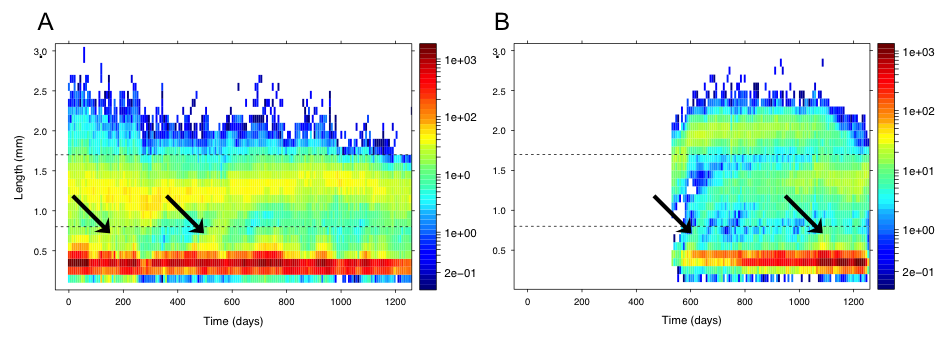
\includegraphics[width=0.95\textwidth]{3-1_ChapExp1/Fig/AnnSP1}
\caption[\lofimage{3-1_ChapExp1/Fig/AnnSP1}Examples of a population's
structure]{Examples of a population's structure - time diagram. A clone TO
replicate r3. B clone HA replicate 15. Dashed lines show the arbitrary
distinction made between juveniles ($<0.8$ mm), small adults ($<1.7$ mm) and
large adults ($>1.7$ mm) on the basis of all the structure time diagrams. Black
arrows mark some of the recruitment periods.}
\label{fig:AnSP1}
\end{center}
\end{figure}

\subsubsection{Size structure dynamics}

 We then look at the size structure dynamics, focusing on short-term events.
Figure \ref{fig:AnSP1}A and B show that although the size structure is rather
stable over time, dynamical processes can be observed on the structure-time
diagrams.

\paragraph{Cohort recruitment}

In Figure \ref{fig:AnSP1}A for instance, we can observe the recruitments of a cohort of
juveniles from the small sizes to the adult class. Such recruitment is
visible between days 450 and 650, and less clear but nevertheless present around
day 200 (black arrows on the diagram). This shows that recruitment in the adult class happens in waves. This dynamical pattern can be observed in every
population we followed, although it is not always very clear.

Figure \ref{fig:AnSP1}B also shows recruitment periods, for instance at 600
days, but this recruitment only goes up to the first class of adult. This observation on the
case study is also valid for every HA population with two separates classes of
adults. When two adults classes coexist in a single population, we
never observe any clear period of recruitment from the first class to the bigger
class of adults (see appendices, populations r5, r7, r9, and 11 to 16).

Furthermore, these recruitment periods are very irregular. Indeed, they can
happen in a relatively short window of time, as in Figure \ref{fig:AnSP1}A, when the two
periods of recruitment are separated by only 200 days. But we also observe very
long periods without any recruitment. On the same figure, the second wave of
recruitment is followed by 500 to 600 days without clear recruitment wave to the
adult class. On the other hand, in certain conditions, recruitment can occur in
a rather regular cycle as for clone TO in population r7 where we can observe a
recruitment wave almost every 100 days.

These periods of recruitment offer a way to measure cohort growth rates by
estimating the slope of the cohort during the recruitment period. The example of
Figure \ref{fig:AnSP1}A between days 500 and 600 gives for the cohort a growth rate estimated
at $5.0\cdot 10^{-3}$ mm$/$d, that is to say 200 days to grow 1mm. This method
can be applied to any structure-time diagram where recruitment periods are distinctly
recognizable. In conditions of populations with sometimes very high densities
where tracking individuals is impossible, such a measure gives an insight into
populations life history traits and trajectories that would else be difficult to
obtain.

\begin{figure}[!ht]
\begin{center}
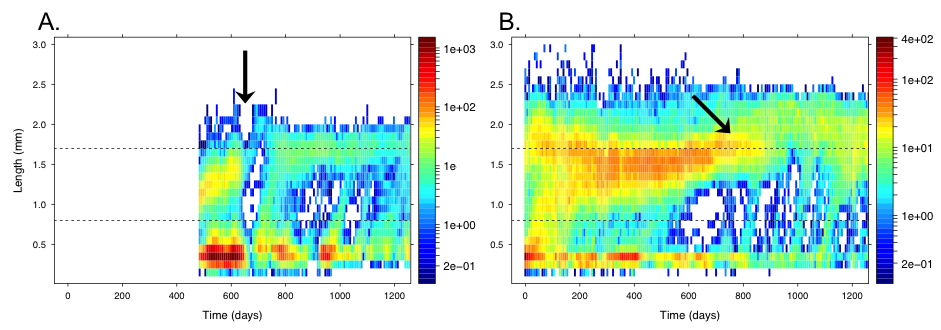
\includegraphics[width=0.95\textwidth]{3-1_ChapExp1/Fig/AnnSP2}
\caption[\lofimage{3-1_ChapExp1/Fig/AnnSP2}Examples of a population's
structure]{Example of a population where a catastrophic event (A, Clone TO
population 11, black arrow) or the senescence of the adult class (B, clone HA
population r4, black arrow) leads to growth of adults and recruitment of cohorts
of juveniles.}
\label{fig:AnSP2}
\end{center}
\end{figure}

Finally, recruitment periods sometimes follow catastrophic events, particularly
in clone TO. Figure \ref{fig:AnSP2}A shows an example of such a catastrophic
event (arrow).
We can observe that at day 670, almost all the population goes extinct except for
few adults. These adults immediately start growing rapidly to reach unusually
large size for clone TO, while a clutch hatches, immediately followed by the
recruitment of a cohort to the adult class. Several other populations of clone
TO present the same kind of catastrophic event followed by growth of remaining
adults and recruitment of a cohort: r6, r8, 12, 13.

Catastrophic events are not the only event that can cause cohort recruitments.
Indeed, the recruitment of a new cohort of juveniles can follow the decline of
the class of adults, as for population HA r4 (Figure \ref{fig:AnSP2}B arrow). Indeed, we can
see that a large number of adults recruits early in the dynamics, up to day 200,
but then remains stable for almost 600 days without recruitment. During this
long period, no recruitment is observed and the cohort of adults is slowly
decreasing in number of individuals with the old individuals dying. Around day
800, the number of adult left is very low, and we observe the recruitment of a
new cohort along with the growth of the remaining adults. This shows that the
aging of the adults can be a driver of the dynamics of the entire population.

\paragraph{Adult size plasticity}

As previously mentioned, we also observe adjustments of the adult body length
during the different dynamic events described. First, we can note that depending
on the demographic context, the adult cohorts stabilize at different body
lengths. The four populations shown as example (Figure \ref{fig:AnSP1} and
Figure \ref{fig:AnSP2}) have four different equilibrium size for the adult
class. The populations of clone TO stabilize between 1 and 1.5mm (Figure
\ref{fig:AnSP1}A) at high density (up to 100 adults and more than 1000
individuals in total) and 1.7mm (Figure \ref{fig:AnSP2}A) at a lower density
($\sim 200$ individuals and about 25 adults), whereas clone HA tends to be
bigger with adults in two classes around 1.5 mm and 2 mm in population 15
(Figure \ref{fig:AnSP1}B) with a population density around 800 to 1000
individuals, around 150 intermediate adults and 50 large ones, and in a single class around 1.7 mm (with
variations up to 2.2 mm) in population r4 (Figure \ref{fig:AnSP2}B) with only few hundred
individuals and few adults ($\sim 50$).

Moreover, adults can rapidly adjust their body length after stabilization in
case of dynamic events that change the population size structure. In the one
hand, in case of the catastrophes described previously, we observed that along
with a recruitment of a new cohort of juveniles, a catastrophic event is often
followed by a resumption of growth of the remaining adults up to $40\%$ of their
current size (Figure \ref{fig:AnSP2}A, adults grow from 1.5 mm up to 2.1 mm).
The same happens if the number of adults decreases due to background mortality
without any recruitment, as in Figure \ref{fig:AnSP2}B around day 800, with the
remaining adults growing from 1.7 mm up to 2.2 mm.

In the other hand, adults also seem to have the possibility to shrink in case
the number of adults quickly increases, for example when a large cohort of
juveniles recruits at the same time. Figure \ref{fig:AnSP2}B shows such a
phenomenon. Indeed, we can see that from day 0 to day 200, the average body
length of the group of adults above 1.5 mm decreases while a large cohort of
juveniles starts growing.
Between days 100 and 200, the size structure is tri-modal, but the large adults
continue to shrink until both classes of adults merge into one big group with a
bigger variability in adult body length. Such shrinking of the adults can be
observed in other population while a cohort recruits, for example in population
HA r1 to r3 and TO r5 and r9.

A summary of the different phenomena described here and the populations and
dates at which they have been observed is given in Table \ref{tab:AnSP1}.

{\tiny
\begin{longtable}{
	p{\dimexpr.12\linewidth-2\tabcolsep-1.3333\arrayrulewidth}% column 1
 	p{\dimexpr.128\linewidth-2\tabcolsep-1.3333\arrayrulewidth}
 	p{\dimexpr.128\linewidth-2\tabcolsep-1.3333\arrayrulewidth}% column 1
 	p{\dimexpr.128\linewidth-2\tabcolsep-1.3333\arrayrulewidth}
 	p{\dimexpr.12\linewidth-2\tabcolsep-1.3333\arrayrulewidth}% column 1
 	p{\dimexpr.12\linewidth-2\tabcolsep-1.3333\arrayrulewidth}
 	p{\dimexpr.126\linewidth-2\tabcolsep-1.3333\arrayrulewidth}% column 1
 	p{\dimexpr.126\linewidth-2\tabcolsep-1.3333\arrayrulewidth}}
 	
\caption{Summary of the state and dynamic observations. The numbers in the table
are the dates or the intervals where to see the event
described.}\label{tab:AnSP1}\\
 	\hline
 	\endhead
 	
\hline
\endfoot

Populations & Trimodal & Long period without recruitment & Frequent recruitment
& Catastrophic event & Adult cohort aging & Adult growing to adjust & Adult
shrinking to adjust\\
\hline\\
HA r1 & - 			& - 		& - 		& - 	& 500  & 500-650  & 650-750  \\
HA r2 & - 			& - 		& - 		& - 	& 800  & 650-900  & - 		 \\
HA r3 & - 			& - 		& - 		& - 	& 800  & 900-1000 & 1000-1250\\
HA r4 & - 			& - 		& - 		& - 	& 800  & 600-1000 & -        \\
HA r5 & 600-1000 	& - 		& - 		& - 	& 1000 & - 		  & - \\
HA r6 & - 			& 800-1250 	& - 		& - 	& -    & - 		  & - \\
HA r7 & 700-1100 	& - 		& - 		& - 	& 1000 & - 		  & - \\
HA r8 & 600-1000 	& - 		& - 		& - 	& 950  & - 		  & - \\
HA r9 & 700-1200 	& 700-1100 	& - 		& - 	& -    & - 		  & - \\
HA 10 & 600-900 	& - 		& - 		& - 	& 900  & - 		  & - \\
HA 11 & 600-1100 	& 700-1250 	& - 		& - 	& 1100 & - 		  & - \\
HA 12 & 600-900 	& - 		& 600-1250 	& - 	& 1000 & - 		  & - \\
HA 13 & 600-1100 	& - 		& 600-1250 	& - 	& 1100 & - 		  & - \\
HA 14 & 600-1100 	& 600-1000 	& - 		& - 	& 1100 & - 		  & - \\
HA 15 & 600-1100 	& - 		& 600-1250 	& - 	& 1100 & - 		  & - \\
HA 16 & 600-1200 	& - 		& - 		& - 	& 1200 & - 		  & - \\
TO r1 & - 			& 400-600 	& 0-400 	& - 	& 400  & 400-600  & -\\
	  &				& 700-1000	& 1000-1250 & 		&	   &		  &\\
TO r2 & - 			& 500-750 	& 0-450 	& - 	& 400  & 500-700  & - \\
	  & 			& 			& 1000-1250 &		&	   &		  &\\
TO r3 & - 			& 600-1250 	& - 		& - 	& -    & - 		  & 0-200\\
TO r4 & - 			& - 		& 0-1250	& - 	& 400  & - 		  & 700-1000\\
TO r5 & - 			& - 		& - 		& 900 	& -    & 900-1000 & 500-700\\
TO r6 & - 			& 600-950 	& - 		& 950 	& -    & 950-1000 & -\\
TO r7 & - 			& - 		& 500-1250 	& - 	& -    & - 		  & -\\
TO r8 & - 			& 600-800 	& 800-1250 	& - 	& 1000 & 1000-1100& -\\
TO r9 & - 			& 600-1000 	& - 		& - 	& 950  & 900-1000 & 500-600\\
TO 11 & - 			& - 		& 700-1250 	& 650 	& -    & 650-750  & -\\
TO 12 & - 			& - 		& - 		& 750 	& -    & 750-850  & -\\
TO 13 & - 			& 500-800 	& 800-1250 	& 800 	& -    & - 		  & -\\

\end{longtable}
}

\subsection{Quantitative analysis of populations dynamics}

We use here a quantitative approach based on the principle component analysis to
simplify our complex dataset into few dimensions, making it easier to comprehend
and manipulate, and to allow for a more thorough statistical analysis of the
dependency of the size structure and its dynamics on diverse factors such as the
genetic lineage or the state itself.

\subsubsection{Principal components}

As described in the methods we decompose our compiled dataset of all our
populations into principal components, without accounting for time dependence.
We use 30 size classes in our dataset going from 0 to 3 mm by steps of 0.1 mm.

\begin{figure}[!ht]
\begin{center}
\includegraphics[width=0.95\textwidth]{3-1_ChapExp1/Fig/AnnSP3}
\caption[\lofimage{3-1_ChapExp1/Fig/AnnSP3}Scree plot of the PCA and
coordinates of first components]{A. Scree plot of the principal component
analysis.
The plain line gives the eigenvalues whereas the dashed line is the cumulative percentage of variance explained. B. Coordinates of the size classes on the first three eigen
vectors.}
\label{fig:AnSP3}
\end{center}
\end{figure}

Figure \ref{fig:AnSP3} shows the cumulative percentage of the variance explained
by the components along with the scree plot of the principal component analysis.
Looking at the eigenvalues, we can see a clear break in the slope after the
first three components. This suggests that keeping only the first three
components to simplify the data is sufficient to explain correctly the different
patterns in size distribution observed in our data. These first three components
represent together $70\%$ of the total variance of our data.

Figure \ref{fig:AnSP3}B shows the coordinates of the original vectors of our data set, that is
to say the size classes, on the first three eigenvectors. This allows seeing
what part of the original distribution is explained by each of the eigenvectors.
We can see that the first components, which explains by itself $43\%$ of the
variance, represents essentially the first half of the size classes, with
individuals smaller than 1.6mm. On the contrary, the second component that
explains $20\%$ of the variance represents both the small adults (0.8 to 1.3 mm)
and individuals bigger than 1.6mm with a major part explained by the larger
ones. Finally, the third component ($7\%$ of the variance) allows
distinguishing between a group of intermediate individuals with a size between 0.8 and 1.9mm,
and the very small individuals (<0.8 mm) and very large individuals (>1.9 mm).

Altogether, the first three principal components of our decomposition give a
good description of the majority of the information present in our data, by
decomposing the size classes into several groups of interest: (i) the juveniles
(<0.6mm), negative on the first axis and positive on the third one, (ii) small
adults (between 0.6 mm and 1.2mm), negative on the first and the third axes and
positive on the second one, (iii) intermediate adults (1.2 mm to 1.9 mm) mostly
negative on the third axis, and (iv) big adults (>1.9 mm) positive on the second
axis. Those four groups describe well the groups identified using the
structure-time diagrams, but without deciding for size classes a priori,
justifying a simplification of our data into four size classes. The number of
individuals in each class gives an idea of the overall size distribution.

As the first two components bare most of the variance ($63\%$), we reduced even
more the data by dropping the third component, keeping only the first two in the
rest of the analysis. This allows a 2D-representation of the structured data on
a phase plane with the two components as axes, with the original vectors
superimposed (biplot). Figure \ref{fig:AnSP4} shows the biplot with a
color-coding of the four major size classes previously described. The third class, the intermediate
adults, has been coded in two different colors depending whether individuals are
bigger or smaller than 1.65 mm, showing that presence of the former will cause a
decrease along the first axis whereas the latter will cause an increase along
the second axis. First, we can see in a different way what have been discussed
with Figure \ref{fig:AnSP3}, that is to say, that the first component represents mostly the
smaller individuals whereas the second one represents the bigger one. But we
observe as well that the data plotted on the first two components spread in four
distinct clusters, indicating four significantly distinct types of size
structures in our dataset.

\begin{figure}[!ht]
\begin{center}
\includegraphics[width=0.95\textwidth]{3-1_ChapExp1/Fig/AnnSP4}
\caption[\lofimage{3-1_ChapExp1/Fig/AnnSP4}Biplot of the principle component
analysis]{Biplot of the principle component analysis with the first two
components. The black dots are the data represented on the first two principle
components (primary x and y axes). The arrows are the original
size classes projected on the first two eigenvectors (secondary x and y axes).
The color-coding represents the four groups previously identified.}
\label{fig:AnSP4}
\end{center}
\end{figure}

\subsubsection{Four groups of size structure}

\begin{table}[!ht]
\centering
\footnotesize
\caption{Structure type characteristics. Average number of
individuals or size in mm and standard error}\label{tab:4types}
\begin{tabular}{rrrrr}
  \hline
Structure  & Total & Number & Number & Number\\
type & abundance & of & of & of \\
  &  & small individuals & large individuals & modes \\
  \hline
  1 & 1286 (sd 662)& 1268 (sd 661)& 18 (sd 10)& 2\\ 
  2 & 202 (sd 148)& 184 (sd 148)& 18 sd(8)& 2\\ 
  3 & 122 (sd 66)& 68 (sd 57)& 54 (sd 22)& 2\\ 
  4 & 490 (sd (291)& 430 (sd 298)& 60 (sd 22)& 3\\ 
   \hline
\end{tabular}
\\[12pt]
\begin{tabular}{rrrrrrr}
  \hline
Structure  & Density & Density
& Density & Size & Size & Size \\
type & in & in & in & of & of & of \\
  & first mode &
 second mode & third mode & first mode & second mode & third mode \\
  \hline
1 & 1113 (sd 648)& 185 (sd 56)& - & 0.37 (sd 0.1) & 1.32 (sd 0.3) & - \\ 
  2 & 145 (sd 143)& 59 (sd 23)& - & 0.42 (sd 0.14) & 1.56 (sd 0.27) & - \\ 
  3 & 40 (sd 51) & 84 (sd 40)& - & 0.39 (sd 0.14)& 1.80 (sd 0.34) & - \\ 
  4 & 340 (sd 295)& 106 (sd 41)& 60 (sd 22)& 0.38 (sd 0.09) & 1.32 (sd 0.29) & 2.02
  (sd 0.23)\\
   \hline
\end{tabular}

\end{table}

We hence used a non-hierarchical clustering method to identify four groups in
the original dataset using the k-means algorithm. Figure \ref{fig:AnSP5} shows the projection
of the four groups on the first two components. We can see that the clustering
analysis conducted on the entire dataset groups well together the four groups
that were visible on Figure \ref{fig:AnSP4}. We plotted together on four structure-time
diagrams the observations from each of the groups to verify the interpretation
of each group in terms of distribution of adults (see supplementary materials).

This representation on the (PC1, PC2) phase plan now gives a quantitative tool
to determine the general structure of a population at a given time, and by
looking at the trajectory in the phase plan over time, a way to analyze the
dynamics across the different characteristic structures.

The different structure types are characterized by the number of modes in the
size distribution, the average length in the different modes and the number of
individuals (Table \ref{tab:4types}). First, we can see that the total abundance
is very different between the different types. Populations in type 1 are much
more dense than others, with a very high density of juveniles (>1000) and the
highest density of adults (185) that remain small (1.32mm). On the contrary,
types 2 and 3 have a low density (202 and 122 total individuals on average).
More precisely, type 2 is described by a skewed distribution in favor of small individuals
(on average 145, 0.42mm) and a low density of intermediate individuals (on
average 59, 1.56mm). Type 3 is described by distribution in favor of large
adults (on average 40 juveniles, 0.39mm against 84 adults, 1.8mm). Finally, type
4 structure have three different modes in the size distribution with a large
number of juveniles (340, 0.38mm), a quite dense group of small adults
(106 individuals, 1.32mm) and a fewer very large individuals (60 individuals,
2.02mm).

\begin{figure}[!ht]
\begin{center}
\includegraphics[width=0.75\textwidth]{3-1_ChapExp1/Fig/AnnSP5}
\caption[\lofimage{3-1_ChapExp1/Fig/AnnSP5}Results of the clustering analysis
with four groups]{Results of the clustering analysis with four groups. The
colors give the interpretation of the groups in terms classes of adults present. The lines show the spatial domain in the (PC1, PC2) space, this domain is then reported in
the trajectories for each population (supplementary materials). For convenience,
the regions are numbered from 1 to 4 as reported on the plot.}
\label{fig:AnSP5}
\end{center}
\end{figure}

\subsubsection{2D representations of the previous examples}

\begin{figure}[!ht]
\begin{center}
\includegraphics[width=0.95\textwidth]{3-1_ChapExp1/Fig/AnnSP6}
\caption[\lofimage{3-1_ChapExp1/Fig/AnnSP6}Time trajectories in the first two principle components]{Time trajectories in the first two principle components.
Colored lines mark the previously identified regions. The triangles mark the
starting points of the four time series. The points are the population
observations. The dotted lines are link the points in time.}
\label{fig:AnSP6}
\end{center}
\end{figure}

Figure \ref{fig:AnSP6} shows the same time series as Figure \ref{fig:AnSP1} (A
and B) and Figure \ref{fig:AnSP2} (C and D), but represented as trajectories in
the main principal components phase plan.

On the one hand, we now have a numerical evidence that shows that population r3
of clone TO spends all its time with a structure composed of juveniles and small
adults, whereas population 11 starts with small adults, but then shifts to a
structure with less juveniles, and intermediate adults. On the other hand, both
populations of clone HA exhibit structures with both small and large adults.
Population 15 starts with a growth period with intermediate adults reaching
large sizes, followed by a long period with both small and large adults, meaning
that new individuals reached adulthood but stayed small. Finally, large adults
died out, driving the trajectory to the small adults region, and finishing with
small adults growing to intermediate adults. The last population always has
large adults. The first part also has small adults that grow into large ones,
shifting the population from the blue to the green region.

\subsubsection{Stability and state transitions in our size structured
population dynamics}

This representation of the time trajectory in a space of the first two principle
components allows determining a date for the transitions from one state to
another, along with a residence time in a given state.

\begin{figure}[!ht]
\begin{center}
\includegraphics[width=0.85\textwidth]{3-1_ChapExp1/Fig/AnnSP7}
\caption[\lofimage{3-1_ChapExp1/Fig/AnnSP7}Time spent in each stable size
distribution region]{Time spent in each stable size distribution region in days
for the two clones merged (A) and separated (B). The letters denote a
significant difference between the corresponding distributions (Tests:
two-sample Kolmogorov-Smirnov test, A: (a) D=0.5, p=0.01, (b) D=0.38, p=0.05,
(c) D=0.51, p=0.002, (d) D=0.43, p=0.03 B: (e) D=0.54, p=0.02, (f) D=0.78,
p=0.0003, (g) D=0.93, p=3x10-6, (h) D=0.53, p=0.03, (i) D=0.67, p=0.04).}
\label{fig:AnSP7}
\end{center}
\end{figure}

Figure \ref{fig:AnSP6} shows four different types of trajectories with different residence
time in the different regions. On Figure \ref{fig:AnSP6}A for instance, we can see that the
population’s structure is very stable and remains the entire 1200 days in the
same region characterizing a structure with juveniles and small adults. In
contrast, Figure \ref{fig:AnSP6}B, C and D show transitions between different regions. More
precisely, population HA 15 (Figure \ref{fig:AnSP6}B) starts in the region with intermediate
adults (red) where it spends about 50 days until it reaches a temporary
equilibrium in the region with both small and big adults for about 550 days,
before going back to the region with intermediate adults. Using the trajectory
in the decomposed space, we can date the first transition at day 57 and the
second one at day 608.

The same analysis can be conducted on each of our 28 populations. First, we look
at the time spent in each region (1 to 4) by each population, corresponding to
the time spent in each of the stable size distributions identified. Figure
\ref{fig:AnSP7}A shows that region 2 is the least stable region with the
smallest amount of time spent in it. This region corresponds to a size distribution with juveniles and
intermediate adults. This region can be seen as a region of transition that is
crossed when going to one of the other stable structures. In contrast, region 4
with a tri-modal distribution is very stable. This is due to the presence of a
cohort of large adults that have a long survival and suffer a low level of
competition, stabilizing the structure. Although the variability is very high in
region 3, the maximums of time spent are in this region, with the same
stabilizing effect of very large individuals. Region 1 is also quite stable and
corresponds to structures where the density is very high causing a big
resilience of the size structure, explaining the relatively long residence time
in it.

Figure \ref{fig:AnSP7}B shows the times of residence in the different regions separated by
clones. We can see in this figure that the patterns of region occupation are
very different depending on the clones. In more details, clone TO spends most of
its time in region 1 and 2 where adults have a small to intermediate body
length, and a very small amount of time with large adults or in a tri-modal
state. Indeed, clone TO is generally smaller than clone HA, and the occurrences
of a type 3 and 4 structure are either due to exceptional conditions followed by
a transition to a type 1 or 2 size structure. On the contrary, clone HA spends
significantly more time in region 3 and 4 than 1 and 2. This confirms the
observations from the qualitative analysis showing that a lot of HA population
exhibited structures with large adults and long lasting tri-modal distribution.
More over this allows us to use the structure type (1 to 4) as a simple rule of
thumb to discriminate between the clones, type 1 and 2 being characteristic
structures of clone TO whereas type 3 and 4 are characteristic of clone HA.


\begin{table}
\small
\centering
\caption{\label{tab:AnSP2}Number of transitions observed in the 28 populations between the different regions. In parenthesis, decomposed between clones HA and TO.}
\renewcommand{\arraystretch}{1.5}% Wider
\begin{tabular}{|rr|cccc|}
\hline 
	&  & & \multicolumn{2}{c}{Region of arrival}  & \\	
	&	& 1 & 2 & 3 & 4 \\
\hline
\parbox[t]{2mm}{\multirow{4}{*}{\rotatebox[origin=c]{90}{Region of origin}}} &
1 & - & 22 (HA: 2, TO: 20) & 0 & 24 (HA: 17, TO: 7) \\
 & 2 & 19 (HA: 4, TO: 15) & - & 26 (HA: 12, TO: 14) & 19 (HA: 8,
TO: 11)\\
 & 3 & 0 & 23 (HA: 10, TO: 13) & - & 32 (HA: 27, TO: 5) \\
 & 4 & 32 (HA: 23, TO: 9) & 17 (HA: 5, TO: 12) & 32 (HA: 26, TO: 6)
& -\\
	
\hline

\end{tabular} 
\end{table}

Table \ref{tab:AnSP2} shows the number of occurrences of each possible
transition between regions in all our time series. First, we can note that two transitions are
never observed. Indeed it is biologically not likely to go from region 1 (small
adults) directly into region 3 (large adults) without going through region 2,
and vice versa, but the number of occurrence of the other transitions is quite
homogeneous. Second, looking at the differences between HA and TO (in
parentheses), we can see that the frequency of each transition is no longer
homogeneous within a given clone. For instance, some of the transitions are very
frequent in clone HA but rare in clone TO (1 $\rightarrow$ 4, 3 $\rightarrow$ 4, 4 $\rightarrow$ 1 and 4 $\rightarrow$ 3), whereas
others are mainly due to clone TO (1 $\rightarrow$ 2, 2 $\rightarrow$ 1). This is due to an intrinsic
difference between the two clones and their life histories that result in
different attractors in term of stable size structures (region 3 and 4 in HA,
regions 1 and 2 in TO).

\section{Discussion}

We have described and quantitatively analysed detailed time series of the
structure of 28 populations of two different clonal lineages (16 populations of
clone HA, 12 of clone TO)

\subsection{Dynamic consequences of genetic differences}

We showed different patterns of size structure states and dynamics that were
observed numerous times in our different populations. Interestingly, the
patterns observed are different depending on the genetic background. The two
clones we studied here (HA and TO) are known for their different life history
strategies \autocites{tully2006a,tully2008a}. Indeed, whereas
clone HA has a low-flexibility strategy that produces small eggs and barely increases its
reproductive investment in response to the environmental amelioration, clone TO
has a high-flexibility strategy, characterized by larger egg size and highly
flexible reproductive investment \autocites{tully2008a}.

The different life history strategies also have consequences on the size
structure states and dynamics of each clone. Indeed, clone HA tends to favour
growth over reproduction, leading to structures with larger adults than clone
TO, which favours reproduction and generally has small adults. Further more, the
ability of clone HA to produce very large individuals explain its ability to
reach a structure of type 4 with a tri-modal distribution. Indeed, when the
conditions are favourable, very large individuals with high survival capacity
emerge in the population. Once settled, they dominate the population and prevent
other adults to reach their size, blocking them at a smaller body length,
causing the third mode in the size distribution to appear.

These consequences of the genetic background show how important it is to know
the life history of the species studied in order to understand the size
structure dynamics that can be observed, and to be able to predict their
possible outcome.

\subsection{The role of initial conditions}

Interestingly, although the type 4 structure seems highly stable, it only
appeared in our populations at the very beginning of the time series. Indeed,
this size structure is locally stable but depends a lot on the initial
conditions to be reached. For a population to reach a type 4 size structure, two
criteria need to be met: (i) the individuals in the population need to be able
to grow quickly and reach a long body size, which is the case of individuals
from clone HA but not TO; (ii) the level of competition needs to be at its
minimum, which translates in the absence of adults in the population and a small
density of juveniles. In these conditions, the juveniles will very quickly grow
to large body size, and impose their dominance on the rest of the population by
monopolizing the resources.

As for the type 4 size structure, the other observed structured are also
dependent on the initial conditions. An artificially high density of juveniles
as initial state will lead to a type 1 size structure whereas a relatively even
size distribution between juveniles, small and intermediate adults will
generally result in a type 2 size structure for clone TO and a type 3 for clone
HA.

The determinant role of initial conditions in the structure state reached by a
population illustrates the coexistence of the four quasi-stable attractors, even
though the breeding conditions are kept the same throughout time for all the
populations. Moreover, the transitions from two stable states are either caused
by the aging of the large adult cohort that disappear, or catastrophic events
that reset the population to new initial conditions and lead it to a new
attractor. Populations in which none of the above occurs remain in the same size
structure during the whole period of measurement, like population TO r3 (Figures
\ref{fig:AnSP1}A and \ref{fig:AnSP6}A) that stays in a type 1 structure during more than 1200
days.

This sensitivity to initial conditions also illustrates clearly the major
importance of including the structure of the population in the analysis of its
dynamics rather than the simple number of individuals. Indeed, with the same
number of individuals, starting a population with small individuals rather than
large ones will have a dramatic impact on the future dynamics of the whole
population, including its potential survival. This confirms previous results
shown by \textcites{benton2005a} on soil mite populations.

\subsection{The role of large individuals on the structure dynamics, an evidence
for interference competition}

Throughout our analyses, we have demonstrated the importance of large
individuals in the dynamics of the size structure of the population. The
resources need to be abundant and the competition for its access as low as
possible for an individual to reach a very large size. If the access to the
resources was only limited by exploitative competition, every individual would
gain access to part of the resource and the energy budget theory predicts that
large sizes are disadvantaged due to higher maintenance rate compared
to smaller individuals \autocites{de-roos2003b}. In these conditions, the
size structure of the populations would inevitably tend to a structure where small individuals
dominate in number and have a size close to their size at maturation, and
emergence of large individuals would be impossible.

In our dynamics, we observed evidences for a more complex regulation system: (i)
in several conditions, large individuals can emerge and survive in the
population, (ii) in cases of catastrophic events, the disappearance of the
larger individuals is immediately followed by the recruitment of a new cohort,
(iii) the aging of cohorts of large adult and their progressive disappearance
also provoke new recruitment periods, and (iv) dense cohort of adults are often
concomitant with long periods without recruitment. These different observations
support a regulation system involving the dominance of the population by the
larger individuals that monopolize the resources, preventing access to the
smaller individuals that stay small. This mechanism can be seen as interference
competition. When the number of large individuals decreases, the competition
pressure put on the smaller ones is progressively released, until the small
individuals gain access to the resource, and along with the remaining large ones
can resume their growth.

Interference competition is believed to be widespread in nature and to play an
important role on populations dynamics. Our study shows that analysing the
temporal dynamics of the size structure of a population rather than its overall
dynamics allows to describe more precisely the mechanisms involved in its
regulation, such as the role of the life history strategies that the individuals
follow, the importance initial conditions and the type of intraspecific
interactions.

We believe that our study is a striking example of how a population dynamics can
be controlled by large individuals that monopolize the resources, giving rise to
different possible structures and complex dynamics that are highly dependent on
the life history of the individuals. Modelling interference competition in a
structured population would allow confirming that with a high enough intensity,
interference competition is sufficient to cause emergence and survival of large
individuals, and dynamics involving multimodal size distributions.

\newpage
\section{Supplementary materials}

\subsection{Structure-time diagrams and 2D time trajectories of each population
studied}

~
\includegraphics[height=0.33\textheight]{3-1_ChapExp1/Fig/HA-21-r1}

\includegraphics[height=0.33\textheight]{3-1_ChapExp1/Fig/HA-21-r2}

\includegraphics[height=0.33\textheight]{3-1_ChapExp1/Fig/HA-21-r3}

\includegraphics[height=0.33\textheight]{3-1_ChapExp1/Fig/HA-21-r4}

\includegraphics[height=0.33\textheight]{3-1_ChapExp1/Fig/HA-21-r5}

\includegraphics[height=0.33\textheight]{3-1_ChapExp1/Fig/HA-21-r6}

\includegraphics[height=0.33\textheight]{3-1_ChapExp1/Fig/HA-21-r7}

\includegraphics[height=0.33\textheight]{3-1_ChapExp1/Fig/HA-21-r8}

\includegraphics[height=0.33\textheight]{3-1_ChapExp1/Fig/HA-21-r9}

\includegraphics[height=0.33\textheight]{3-1_ChapExp1/Fig/HA-21-10}

\includegraphics[height=0.33\textheight]{3-1_ChapExp1/Fig/HA-21-11}

\includegraphics[height=0.33\textheight]{3-1_ChapExp1/Fig/HA-21-12}

\includegraphics[height=0.33\textheight]{3-1_ChapExp1/Fig/HA-21-13}

\includegraphics[height=0.33\textheight]{3-1_ChapExp1/Fig/HA-21-14}

\includegraphics[height=0.33\textheight]{3-1_ChapExp1/Fig/HA-21-15}

\includegraphics[height=0.33\textheight]{3-1_ChapExp1/Fig/HA-21-16}

\includegraphics[height=0.33\textheight]{3-1_ChapExp1/Fig/TO-21-r1}

\includegraphics[height=0.33\textheight]{3-1_ChapExp1/Fig/TO-21-r2}

\includegraphics[height=0.33\textheight]{3-1_ChapExp1/Fig/TO-21-r3}

\includegraphics[height=0.33\textheight]{3-1_ChapExp1/Fig/TO-21-r4}

\includegraphics[height=0.33\textheight]{3-1_ChapExp1/Fig/TO-21-r5}

\includegraphics[height=0.33\textheight]{3-1_ChapExp1/Fig/TO-21-r6}

\includegraphics[height=0.33\textheight]{3-1_ChapExp1/Fig/TO-21-r7}

\includegraphics[height=0.33\textheight]{3-1_ChapExp1/Fig/TO-21-r8}

\includegraphics[height=0.33\textheight]{3-1_ChapExp1/Fig/TO-21-r9}

\includegraphics[height=0.33\textheight]{3-1_ChapExp1/Fig/TO-21-11}

\includegraphics[height=0.33\textheight]{3-1_ChapExp1/Fig/TO-21-12}

\includegraphics[height=0.33\textheight]{3-1_ChapExp1/Fig/TO-21-13}


 



\chapter[Interférence vs. exploitation et dynamique des populations
structurées][Interférence et populations structurées]{Interférence vs.
exploitation et dynamique des populations structurées}
\label{An:AmNat}

\vspace{2cm}
\begin{Spacing}{1}
\texttt{
Le Bourlot, Vincent, Thomas Tully and David Claessen, "Interference versus
Exploitative Competition in the regulation of Size-Structured Populations"\\
under review at The American Naturalist
}
\end{Spacing}


\section*{Abstract}
\addcontentsline{toc}{section}{Abstract}

\lettrine[lines=3]{C}{ompetition is a major} regulatory factor in population
and community dynamics.
Its effects can either be direct in interference competition, or indirect in
exploitative competition. The impact of exploitative competition on population
dynamics has been extensively studied from empirical and theoretical points of
view but the consequences of interference competition remain poorly understood.
Here we study the effect of different levels of intra-specific interference
competition on the dynamics of a size-structured population. We study a
physiologically structured population model accounting for direct individual
interactions, allowing for a gradient from exploitative competition to
interference competition. We parameterize our model with data on experimental
populations of the Collembola \textit{Folsomia candida}. Our model predicts
contrasting dynamics depending on the level of interference competition. With low
interference, our model predicts juvenile-driven generation cycles, but
interference competition tends to dampen these cycles. With intermediate
interference, giant individuals emerge and start dominating the population.
Finally, strong interference competition causes a novel kind of adult-driven
generation cycles referred to as “interference-induced cycles”. Our results shed
new light on the interpretation of the size-structured dynamics of natural and
experimental populations.

\section{Introduction}

Competition is one of the most important ecological interactions that structure
populations and communities and is defined as an interaction between organisms
such that the performance in terms of fecundity, growth rate and survival, is
reduced by the presence of other organisms
\autocites{volterra1931a,gause1932a,park1948a,park1954a,park1957a}. Two types of
competition are distinguished:
exploitative (or scramble) competition and interference (or contest) competition
\autocites{park1954a,park1962a,begon2009a}. Competition is exploitative when
individuals have a negative effect on each other by draining a common resource
\autocites{goss-custard1980a,vance1984a,begon2009a}. This process causes a
decrease of the individuals’ intake rates because resources such as food,
nutrients or mates \autocites{begon2009a} are depleted by the presence and activity
of other individuals. Exploitative competition is indirect because it does not
require any physical interaction between the competing individuals and can only
occur if the resource considered is limiting \autocites{begon2009a}.

By contrast, interference competition happens when individuals experience direct
negative interactions where one individual reduces the other’s ability to
exploit a common resource regardless of its level
\autocites{park1954a,vance1984a}.
These interactions involve aggressive displays \autocites{schoener1976a},
territoriality (salamanders: \textcite{walls1990a}; wrens:
\textcite{kennedy1996a}), allelopathy (\textcite{harper1977a,rice1984a};
Empetrum: \textcite{nilsson1994a}), overgrowth (barnacle:
\textcite{connell1961a,paine1966a}), etc.
Interference competition reduces the performance of the inferior competitors by
denying them access to resources \autocites{schoener1983a,thompson1993a}.
Dominance in interference competition is often determined by differences in body
size between competitors, the larger having usually superior competitive
abilities \autocites{mccormick2012a}. This means that for the case of
intra-specific interference the occurrence and consequences of competition
generally depend on the population’s size distribution, and the life-history
states (i.e., current body size) of the individuals.

Interference competition has been widely observed in nature either between
species or within species, but only few theoretical studies have assessed its
effect on population and community dynamics. Most of these theoretical studies
focus on inter-specific interference competition
\autocites{case1974a,carothers1984a,vance1984a,adler2000a}. An interpretation of
interference competition is given in the formulation of the Arditi-Ginzburg
ratio-dependent model \autocites{arditi1989a,arditi1991a,arditi2012a}. In this
model, the yearly consumption rate of prey by predators depends on the prey
abundance per capita of predators rather than the absolute abundance of prey.
That ratio dependence leads to different kinds of behavior compared to the
standard Rosenzweig-MacArthur model in which the kill rate is only limited by
the density of prey. The paradox of enrichment is for instance absent from the
ratio-dependent model \autocites{arditi2012a}. Other studies propose different
approaches. \textcite{amarasekare2002a} presents a model of exploitative and
interference competition with explicit resource dynamics to study the possible
coexistence of two competing species. The study shows that, when interference
competition is costly, the two competing species cannot coexist, even if the
species that is dominated in exploitative competition dominates its competitor
through interference competition. In contrast, the authors show that species
coexistence is possible when exploitative inferiority balances with interference
superiority and when interference competition is beneficial for the superior
competitor.

Interference competition can also be intra-specific
\autocites{walde1984a,crowley1987a,maddonni2004a,smallegange2006a}.
\textcite{de-villemereuil2011a}, studied different consumer functional
responses, extending existing functional response models to account for both
intra- and inter-specific interference behaviors, showing in their case study
that intra-specific interference is more effective than inter-specific
competition in regulating population dynamics.

The sign and strength of interference competition is usually determined by
life-history differences between individuals (differences in body size, sex,
strength, etc) and therefore modeling the population dynamics of interference
competition requires an individual-based approach. Physiologically structured
population (PSP) models are particularly well suited for studies on
intra-specific competition since they account explicitly for the population size
distribution and derive the population dynamics from the individual-level
processes such as growth, reproduction and mortality
\autocites{kooijman1984a,metz1986a,de-roos1997a}. Moreover, because PSP models
include ontogenetic development, it is possible to account for size-dependent
competitive interactions. The theoretical framework of PSP models has been well
developed during the last two decades
\autocites{de-roos1992a,de-roos1997a,persson1998a,de-roos2001a,diekmann2001a,
diekmann2007a,de-roos2012a}, and the models have been applied to a variety of
topics such as size-dependent competition \autocites{persson1998a},
size-dependent predation \autocites{wolfshaar2006a}, cannibalism
\autocites{claessen2000a,claessen2004a}, or the impact of temperature on
population dynamics \autocites{ohlberger2011a}.
These studies have led to the development of a paradigm of population and
community dynamics, taking into account the consequences of ontogenetic
development \autocites{de-roos2012a}. Previous studies of structured-population
dynamics have shown a number of possible dynamical behaviors
\autocites{de-roos2003a,de-roos2003b}. In particular, in a population regulated
only by exploitative competition, the competitive abilities of small versus
large individuals will determine the type of dynamics observed. For many species
size-dependent scaling is such that exploitative competition favors small
individuals by assuring them an energetic advantage
\autocites{persson1998a,persson2006a}, in which case the competitive asymmetry in
their favor leads to juvenile-driven population cycles (also referred to as
single-generation cycles, \textcite{murdoch2002a}), with waves of recruitment
causing oscillations \autocites{de-roos2003a,de-roos2003b}. A competition balance
in favor of large individuals leads to adult-driven cycles, whereas with an even
balance, the dynamics converges to a fixed point with a stable size distribution
\autocites{de-roos2003a,de-roos2003b}.

To date, the consequences of interference competition in size-structured
populations remain unexplored – cannibalism, predation and exploitative
competition being the only interactions considered so far. Here, we propose an
extension of the classical Kooijman-Metz model
\autocites{kooijman1984a,de-roos1997a} by explicitly incorporating interference
competition. We consider interference as a direct interaction between two
contestants where the advantage is given to the largest individual, reducing the
smaller one's access to the resource. We allow for a gradient of competition
from purely exploitative competition to almost pure interference. We aim to
understand the implications of intraspecific interference competition on
population dynamics, using the well-known effect of exploitative competition as
a reference.

We use experimental populations of the Collembola Folsomia candida bred in small
rearing boxes, with weekly resource input \autocites{tully2008a} to calibrate and
test our model. F. candida is a very convenient model species for studying
population dynamics, life history traits and phenotypic plasticity
\autocites{tully2005a,tully2008a}. Easy to breed and manipulate
\autocites{fountain2005a}, it allows for both fine determination of individual
rates and life history traits, and detailed population surveys with individual
body length and population size structure. Our experimental populations are
censused weekly for population abundance and size structure
\autocites{mallard2012a,mallard2013a}. Given their environmental conditions and
the resource availability, our experimental populations exhibit size structure
dynamics that classical exploitative competition models cannot explain. In this
study, we investigate how the level of interference competition influences the
dynamics predicted by the model, and whether accounting for interference
competition can predict population dynamics similar to the ones observed in our
experimental populations.



\section{Methods}

\subsection{Individual level methods}

Our physiologically structured model is based on the model developed by Kooijman
and Metz (KM-model, \citeyear{kooijman1984a}) and \textcite{de-roos1992a}. We
parameterized the model for the Collembola Folsomia candida with data collected
in the laboratory during long-term population surveys. All parameters used in
the model are summarized in Table \ref{tab:param}.

Experimental data on individual-level characteristics show that the important
assumptions of the KM-model are satisfied for this species as described in the
supplementary materials (see 5.1). The major model assumptions are (i) for a
constant food level the model predicts Von Bertalanffy growth curves, while the
maximum size and the growth rate both depend on food level (Figure
\ref{Fig4-SM1}); reproduction increases with the food level and scales with the
square of body length (Figure \ref{Fig4-SM2}). The size at birth is independent
of food conditions (Figure \ref{Fig4-SM3}). Maturation occurs upon reaching a
maturation size (Figure \ref{Fig4-SM4}). Although there is some variation in maturation
length with food availability, the major model assumptions are valid for F.
candida supporting our choice for the KM-model. The KM-model assumes constant
background mortality as a function of length, whereas background mortality in
our experimental populations decreases with length and increases with age. We
have tested that this assumption does not qualitatively affect the obtained
results.

\begin{table}
\caption{\label{tab:param}Variables and parameters for the \textit{Folsomia candida}}
\begin{tabular}{cccl}
\hline
\hline 
 & & &\\
 Objects and  & Default values & Units & Description\\ 
symbols & & &\\
\hline
	$i$-state variable & & & \\ 
	$l$ &   & mm & Individual length \\ 
	Parameters & & & \\ 
	$l_{b}$ & 0.25 & mm & Length at birth \\ 
	$l_{j}$ & 0.6 & mm & Length at maturity \\ 
	$l_{m}$ & 3.0 & mm & Length at infinite\\
	& & &  resources \\ 
	$\gamma$ & 0.015 & d$^{-1}$ & Van Bertalanffy growth rate \\ 
	$\eta_{H}$ & 1000 & individuals & Half saturation constant \\ 
	$\mu$ & 0.0065 & d$^{-1}$ & Background mortality \\ 
	$r_{m}$ & 3.0 & d$^{-1}$mm$^{-2}$ & Reproduction rate \\ 
	$\kappa$ & 0.7 & -- & Fraction of energy \\
	  &   &   & intake allocated \\
	  &   &   & to reproduction \\ 
	  $I$ & 0 & -- & Level of interference\\
\hline 
\end{tabular} 
\end{table}


\begin{table}
\centering
\caption{\label{tab:Eq} Model equation under the $\kappa$-rule.}
\begin{tabular}{cl}
\hline 
\hline
&\\
Equation & Description \\
\hline
	$\displaystyle{A(t,l)=1-\frac{\eta(t,l)}{\eta_{H}+\eta(t,l)}}$ & Access to the
	resource\\
	&\\
	$\displaystyle{\eta (t,l) = \int\limits_{l_b}^{l_m} C(l,\lambda)\cdot
	n(t,\lambda)\cdot \lambda^2\,\text{d}\lambda}$ & Experienced population
	density\\
	&\\
	$\displaystyle{C(l,\lambda) = \text{max}[0.01,\, 1+I\cdot(\lambda-l)]}$ &
	Competition function \\
	&\\
	$\displaystyle{g(t,l) = \gamma\cdot(l_m \cdot A(t,l)-l)}$ & Growth rate\\
	&\\
	$\displaystyle{b(t,l) = r_m \cdot A(t,l)\cdot l^2}$ & Birth rate if $l\geq
	l_j$\\
	&\\
	&\\
	$\displaystyle{\frac{\partial n(t,l)}{\partial t}+ \frac{\partial
	g(t,l)\cdot n(t,l)}{\partial l} = -\mu \cdot n(t,l) }$ & Population level
	equation\\
	&\\
	$\displaystyle{g(t,l_b)\cdot n(t,l_b) = \int\limits_{l_b}^{l_m} b(t,l)\cdot
	n(t,l) \, \text{d}l}$ & Boundary conditions \\
\hline 
\end{tabular} 
\end{table}

\subsubsection{Density dependence}

We use individual length $l$ as the individual state ($i$-state) variable,
ranging from length at birth $l_b$ to a maximum achievable length $l_m$ for
unlimited resources and no competition. Instead of explicit resource dynamics
resulting in exploitative competition, we describe direct individual
interactions explicitly with a function denoted by $A(t,l)$. The function
$A(t,l)$ is referred to as an individual's “access to the resource” which is
supposed to depend on the current population density as experienced by this
individual. We assume that the experienced population density $\eta(t,l)$
depends on an individual's own body size $l$: small individuals suffer from the
presence of large ones more than the inverse. By tuning some parameters,
$A(t,l)$ allows us to model a gradient going from purely exploitative
competition to almost purely interference competition as explained thereafter.
Access to the resource is defined as follows:
\begin{equation}
\label{eq_1}
A(t,l)=1-\frac{\eta(t,l)}{\eta_H+\eta(t,l) }  
\end{equation}

This formulation results in a shape similar to a classical Holling type II
functional response \autocites{holling1965a}. Here $eta_H>0$ is a half 
saturation constant. The experienced population density $eta(t,l)$ is a measure
of how the environment is felt by an individual of size $l$ at a given time $t$:
\begin{equation}
\label{eq_2}
\eta(t,l)=\int_{l_b}^{l_m} \! C(l,\lambda)\cdot n(t,\lambda)\cdot\lambda^2\, \mathrm{d}\lambda
\end{equation}

The quantity $\eta(t,l)$ hence depends on the size distribution of the
population at time $t$, $n(t,\lambda)$, weighted by the squared length
$\lambda^2$ of each individual in the population, and a competition function
$C(l,\lambda)$. The competition function $C$ represents the competitive
superiority of an individual of size $l$ over another one of size $\lambda$,
depending on the difference in length $\lambda-l$:
\begin{equation}
\label{eq_3}
C(l,\lambda) = \mathrm{max}\left[ 0.01,\, 1+I\cdot(\lambda-l) \right]
\end{equation}
where the parameter $I$ is referred to as the interference factor. If $I=0$,
then $C=1$ for every combination of $l$ and $\lambda$, meaning that there is no
interference competition but exploitative competition only. The function $\eta$
then simplifies into
\begin{equation}
\label{eq_4}
\eta (t,l) = \eta(t) = \int_{l_b}^{l_m} \! n(t,l)\cdot l^2\, \mathrm{d}l
\end{equation}
and access $A(t,l)$ then no longer depends on body size; access to the resource
is identical for all individuals. A numerical investigation comparing our model
using $A(t,l)$ with $I=0$ with the original KM-model with explicit resource
dynamics and a type II functional response showed that the dynamics of these
models are nearly identical.

For any positive value of $I$, the access to the resource $A(t,l)$ becomes size
dependent. If an individual $\alpha$ has a length $l_{\alpha}$ and interacts
with an individual $\beta$ of length $l_{\beta}$, we can see from \eqref{eq_1}
and \eqref{eq_3} that $l_{\beta}>l_{\alpha} \Rightarrow
C(l_{\alpha},l_{\beta})>1$, $\beta$ is competitively superior to $\alpha$, and
the environment $\eta(t,l_{\alpha})$ felt by $\alpha$ is more challenging than
$\eta(t,l_{\beta})$, the one felt by $\beta$ (see Figure \ref{Fig4-SM12}).
Moreover, the larger $I$, the steeper the competitive relationship between two
individuals. Tuning the parameter $I$ thus allows us to have a continuous
gradient of competition from purely exploitative competition for $I=0$ to very
strong interference competition for high values of $I$.

The other individual level equations are the same as in Kooijman and Metz
(KM-model, \citeyear{kooijman1984a}) and \textcite{de-roos1992a}, are detailed
in supplementary materials (Sup. Mat. \ref{subsec:SupMat2}) and are
summarized in Table \ref{tab:Eq}.

\subsubsection{Minimum sustainable access to the resource}

Having defined the densitqy dependence relations and individual rates in the
model, we define the minimum required accessibility $A^*$ as the minimum amount
of resources an individual needs to access to be able to maintain itself. $A^*$
is set as the access to the resource at which growth is null:
\begin{equation}
\label{eq_8}
A(l)=A^* (l) \Leftrightarrow g(l)=0
\end{equation}
which leads to 
\begin{equation}
\label{eq_9}
A^*(l) = \frac{l}{l_m}
\end{equation}

Then, for any individual, if $A(l)<A^* (l)$, growth stops and the individual
starves until conditions improve or it dies. That way, $A^*$ is analogous to
Tilmann's $R^*$ in the sense that it determines a minimum condition for growth
\autocites{tilman1982a}, except that $A^*$ is size-dependent (see also
\textcite{persson1998a}).

Population level integration of the model is the same as described in
\textcite{kooijman1984a} and \textcite{de-roos1997a}. Numerical simulations and
analysis have been conducted using the Escalator Boxcar Train (EBT) method
\autocites{de-roos1988a} with the latest available version of
EBTtool (http://staff.science.uva.nl/aroos/EBT/Software/index.html).

\subsection{Sample dynamics}

Several exploratory simulations were conducted for different values of
interference $I$ and background mortality $\mu$ to identify different types of
dynamics. Every simulation lasted $10000$ units of time, with the transient
period lasting at most $2000$ units of time in the longest case. In particular,
we looked at the size structure of the population and several life history traits at the
end of each simulation, such as maximum realized length, and growth rates and
access to the resource as functions of body length. In case of a limit cycle, we
measured the amplitudes of the cycles and their periods, as well as the dynamics
of the size structure.

\subsection{Bifurcation analysis}

To study more precisely how the level of interference $I$ and the mortality
$\mu$ affect the population dynamics, we ran a series of bifurcation analysis
over the parameter space $(I,\mu)$.

In our case, a bifurcation analysis consists of a series of numerical
simulations with all parameters fixed but one, called the bifurcation parameter.
The first simulation is run with the initial value of the bifurcation parameter
until it reaches a stable equilibrium or a limit cycle. The final state of the
population (its distribution at the end of the run) is then used as initial
conditions for a new simulation with the same set of parameters, except for the
bifurcation parameter, which is incremented or decremented. This process is
repeated until the bifurcation parameter reaches the last value. We performed
four different sets of bifurcation runs. (i) The first set had the interference
parameter $I$ as bifurcation parameter, increasing from $0$ to $3$. The set
consists of a large number of such bifurcations runs for fixed values of $\mu$
between $0.001$ and $0.02$. (ii) The second set is the same as the first, except
that the bifurcation parameter $I$ from $3$ to $0$. Comparing results from sets
$1$ and $2$ allows us to detect alternative stable states (bistability). (iii)
The third set of bifurcations has $\mu$ as bifurcation parameter, increasing
from $0.001$ to $0.02$, for fixed values of interference between $0$ and $3$.
(iv) The fourth set is as the third one but with $\mu$ decreasing from $0.02$ to
$0.001$.  With these four sets of bifurcation runs, the parameter space
$(I,\mu)$ was explored in the up-direction and the down-direction.

\section{Results}

First we studied the impact of the level of interference competition on the
individual's maximum observed length (Figure \ref{Fig4-1}A) and on the total population
dynamics (Figure \ref{Fig4-1}B) for a low value of background mortality,
$\mu=0.0065$.

\begin{figure}[!ht] % Figure 1 
\centering
\includegraphics[width=0.85\textwidth]{4_ChapThe1/Fig/Fig1.pdf}
\caption[\lofimage{4_ChapThe1/Fig/Fig1.pdf}Bifurcation over interference]{
Maximum achieved length (A) and total population's extremes (number of
individuals) (B) for increasing values of interference and a low mortality rate
($\mu=0.0065$). Dashed lines mark conditions presented in Figures \ref{Fig4-2}
and \ref{Fig4-3}.
In the bottom plot, thick black lines represent the population's extrema for
each simulation of different values of $I$. The gray areas represent regions
where the population dynamics converges toward a limit cycle. The arrow marks
the transition observed on the top figure.}
\label{Fig4-1}
\end{figure}

Figure \ref{Fig4-1}A shows a very abrupt increase of the maximum length at a
critical value of $I = 1.4$. Below the critical value the maximum achieved
length in the population is just above the length at maturity $l_j=0.6$ mm
($l=0.63$ mm). Above the critical value, the maximum length is close to the
physiologically maximum length $l_m=3$ ($l=2.85$ mm). Interestingly there is no
bi-stability around this critical value.

Figure \ref{Fig4-1}B shows three overall regions of interest: a limit cycle at
low interference, a stable equilibrium at intermediate interference; and a new
limit cycle at high interference. In a small region of interference (around $I =
1.8$) the latter limit cycle has a double period (Sup. Mat. \ref{subsec:SupMat3} and
Figure \ref{Fig4-SM6}) and it becomes irregular at high interference.

\subsection{Juvenile-driven generation cycles}

Without interference ($I=0$), the population converges to a limit cycle that
corresponds to the well-known juvenile-driven generation cycles caused by
exploitative competition \autocites{de-roos1992a,de-roos1997a}. Figure
\ref{Fig4-2} shows a sample dynamics for low interference ($I=0.5$, Figure
\ref{Fig4-2}A,B,C) corresponding to the first dashed line in Figure
\ref{Fig4-1}. Figure \ref{Fig4-2}A presents both the total population dynamics
and the dynamics of its size-structure. These oscillations correspond to
successive waves of cohorts that grow until reaching a reproductive state for a
length $l\geq0.6$ mm. Adults stop growing after reaching maturation, with a
maximum achieved size of $l=0.63$ mm. This is characteristic of juvenile-driven
generation cycles due to exploitative competition
\autocites{de-roos1992a,de-roos2003b}. Figure \ref{Fig4-2}B and C show
respectively the growth rate and the access to the resource as a function of
length. In a purely exploitative competition model, the growth rate is linearly
decreasing with length, and the resource accessibility is constant.
Figure \ref{Fig4-2}B shows that the growth rate is almost linearly decreasing,
although curved upward for $l$ close to $l_j$ ($0.6$ mm), and the access to the
resource is slightly increasing with body size but drops below the minimum
required access $A^*$ (slanting line) for $l > l_j$. The curvature of the growth
rate and the resource accessibility is due to interference competition favoring
bigger individuals.

\begin{figure}[!ht] % Figure 2 
\centering
\includegraphics[width=0.85\textwidth]{4_ChapThe1/Fig/Fig2.pdf} 
\caption[\lofimage{4_ChapThe1/Fig/Fig2.pdf}Sample dynamics for $I=0.5$ and
$I=2.0$]{Sample dynamics for $I=0.5$ (A,B,C) and $I=2.0$ (D,E,F). A and D shows the dynamics of
the total population size along with the dynamics of the structure of the
population \autocites{mallard2012a}. B and E represent the growth rates as a
function of length. The vertical dashed line marks the length at maturity, the
horizontal one the $0$ growth rate. Shaded gray lines show phase lines at
different times, and the thick black line is the average growth. C and F show
the resource accessibility as a function of length. The vertical line marks the
length at maturity. The slanting line is the minimum required accessibility
$A^*$. As for B and E, shaded gray lines and thick black lines represent
respectively the different phase lines and the average competition. The dashed
lines represent the analytical projections of $A$ and $g$ over the whole length
range considering the actual state of the population.}
\label{Fig4-2}
\end{figure}

\subsection{Stable equilibrium with small or giant adults}

With intermediate interference the dynamics tend to a stable equilibrium (Figure
\ref{Fig4-1}B). The explanation is that the size-advantage of adult individuals
due to interference reduces the exploitative competition inflicted by the small
ones, thus undoing the mechanism responsible for the juvenile-driven generation
cycles.

The resulting stable equilibrium can be characterized by either a narrow or a
wide population size distribution (Figure \ref{Fig4-3}). For values below the
critical interference level ($I<1.4$, Figure \ref{Fig4-1}A), the curvature of
the growth rate and the resource access functions is insufficient to allow
growth beyond the size at maturation (Figure \ref{Fig4-3}B,C). In this case, an
immigrant of sufficient body size would have a largely positive growth rate and
reach giant sizes, but the individuals born in the population cannot grow into
this size interval.

Beyond the critical interference level ($I>1.4$, Figure \ref{Fig4-3}D,E,F) the
curvature is just strong enough for individuals to experience a secondary
acceleration of their growth rate, eventually reaching giant sizes (Figure
\ref{Fig4-3}D,E). The population size distribution is strongly skewed since the
growth rates stalls around the maturation size. We refer to the minimum of the
growth rate function as the “growth bottleneck”. The rapid increase in growth
rate and resource access beyond the growth bottleneck ($l>0.65$ mm; Figure
\ref{Fig4-3}F) is explained by the increased competitiveness and by the low
density of large individuals. The linear decrease beyond $l=1.3$ mm is due to
the natural shape of the Von Bertalanffy growth function (Sup. Mat.
eq. \eqref{eq:7}).

\begin{figure}[!ht] % Figure 3 
\centering
\includegraphics[width=0.85\textwidth]{4_ChapThe1/Fig/Fig3.pdf} 
\caption[\lofimage{4_ChapThe1/Fig/Fig3.pdf}Sample dynamics for $I=1.35$ and
$I=1.45$]{Size distributions (A,D), growth rate (B,E) and accessibility (C,F)
for two conditions of interference producing fixed points, $I=1.35$ (A,B,C) and
$I=1.45$ (D,E,F). The dotted and dashed lines are the same as in Figure
\ref{Fig4-2}.}
\label{Fig4-3}
\end{figure}

Figure \ref{Fig4-1}B shows that beyond $I = 1.56$ interference competition
results in population cycles. Figure \ref{Fig4-2}D, E and F show the details of
a sample run for $I=2.0$. Figure \ref{Fig4-2}D shows that these cycles are
different from the juvenile-driven generation cycles (Figure \ref{Fig4-2}A):
the period of the cycles is almost three times longer and the amplitude is about
$7.5$ times larger. The initial increase in population size corresponds to a
birth pulse due to a cohort of individuals reaching maturity ($l \geq l_j$). At
this moment the population is multi modal and composed of a large number of
immature individuals some newly recruited adults and a few old giant
individuals. This birth pulse is followed by the growth of the recently matured
individuals towards giant body sizes, which decreases the resource accessibility
of the smaller individuals that temporarily stop growing (Figure \ref{Fig4-2}D).
The stalling individuals form two distinct groups: juveniles with $l<0.35$ mm;
and juveniles and adults with $0.5 < l < 0.75$ mm (Figure \ref{Fig4-2}D). During
this period, adults continue to reproduce, increasing the abundance of
juveniles. Due the loss of large individuals, the resource accessibility of
intermediate individuals increases allowing them to progressively grow and reach
giant sizes themselves.
The smallest group remains stalling at small sizes and do not mature. The number
of reproducing individuals slowly decreases due to background mortality, leading
to a decrease in total population size and interference competition. When the
number of adults is low enough, the smaller individuals can start growing again
and reach maturity, leading to a new cycle.

Figure \ref{Fig4-2}E and F show respectively the growth rates and the
accessibility against the length with an interference of $I=2.0$, at different
moments of the cycle (in thin gray lines) and on average (thick black lines).
Individuals with a negative growth rate simply stop growing, and suffer
increased mortality if they are not able to fulfill their maintenance. First, we
see on panel E that the position of the growth bottleneck varies on the x-axis
between $0.33$ and $0.55$ mm, depending on the moment considered in the cycle,
but it always happens at a length smaller than the length at maturity, causing
the accumulation of immature individuals.


The resource accessibility (Figure \ref{Fig4-2}F) shows the same phenomenon,
while accumulating at a size smaller than $l_j$, individuals have an
accessibility below the minimum sustainable value, which explains the negative
growth rate (growth stops and mortality is increased). In the phase of the cycle
where the number of large individuals decreases, the resource accessibility of
the smaller ones increases until becoming sustainable again, and they start
growing again. It is the position of the growth bottleneck below $0.6$ mm that
causes the cycling dynamics.

\subsection{\texorpdfstring{$(I,\mu)$}{(I,mu)} Bifurcation}

The previous examples show the behavior of the model for a relatively low
mortality ($\mu=0.0065$). Yet, mortality is known to have a very important role
in the regulation of the dynamics of structured populations. Figure \ref{Fig4-4}
shows the results of bifurcation runs conducted in the $(I,\mu)$ parameter
space. The upward and downward runs gave identical results suggesting the
absence of bistability.

\begin{figure}[!ht] % Figure 4 
\centering
\includegraphics[width=0.85\textwidth]{4_ChapThe1/Fig/Fig4.pdf}
\caption[\lofimage{4_ChapThe1/Fig/Fig4.pdf}$(I,\mu)$ stability
diagram]{Compiled bifurcation diagram in the mortality -- interference
parameter plane. Regions without hatching correspond to regions of stability. White area:
small maximum size. Grey area: giant maximum size. Hatching: type of population
cycle. No bistability was observed. Dashed line: the transect in Figure
\ref{Fig4-1}. Black dots: the locations of the runs in Figure \ref{Fig4-2} and
Figure \ref{Fig4-3}.}
\label{Fig4-4}
\end{figure}

First, Figure \ref{Fig4-4} shows that the parameter space can be separated in
two distinct areas, characterized by either a small ($l=0.63$ mm, white
background) or giant maximum size ($l=2.85$ mm, grey background). The critical
interference level separating these regions is relatively insensitive to the
background mortality ($I \approx 1.2-1.6$).

Second, conform to the theory on exploitative competition
\autocites{de-roos1997a}, increasing background mortality without interference
competition ($I = 0$) tends to stabilize the juvenile-driven generation cycles.
With positive interference competition, the stabilization of these cycles occurs
at a lower mortality rate.
Interference-induced cycles tend to stabilize as well at very high mortality
($>0.02$), but the pattern differs.

At low mortality ($\mu<0.005$) but high interference, the dynamics become
irregular and the size structure exhibits discontinuities. At low mortality and
intermediate interference, between $1.5$ and $2.0$, the situation is more
complex. Indeed, in this region, generation cycles continue to exist although
adults start reaching a length close to $l_m$. But in this region, the
generation cycles are degenerate and some individuals exceptionally manage to
escape the trap of reduced growth rate close to the maturation size and manage
to start growing again, but they are very isolated and the size structure
dynamics is very irregular.

\section{Discussion}

We have shown that interference competition in favor of large individuals is an
interaction that counteracts the consequences of (size-dependent) exploitative
competition. Exploitative competition generally favors small individuals due to
the energetic advantage of a small body size which results from the size scaling
of food intake and maintenance rates
\autocites{peters1986a,persson1998a,de-roos2013a}. This is predicted for most
species by Dynamic Energy Budget theory \autocites{kooijman2000a} and has been
confirmed for the few species for which sufficient empirical data are available
(roach, perch, Daphnia, vendace; De Roos and Persson \citeyear{de-roos2013a}).
Across the gradient of interference competition that we consider (Figure
\ref{Fig4-1}) the overall competitive asymmetry changes gradually from superior
juveniles (due to exploitative competition) to superior adults (due to
interference). In between, the two types of competition more or less balance
each other. Dynamically, this leads to transitions from juvenile-driven
generation cycles to a stable equilibrium to adult-driven generation cycles
(Figure \ref{Fig4-1}).
Interestingly, this pattern is qualitatively similar to the consequences of
varying the size-dependent scaling of exploitative competition in order to give
an energetic advantage to large individuals (without interference competition),
as investigated by \textcite{persson1998a} and \textcite{de-roos2003a}.
The same transitions are found when increasing the slope of the allometric
attack rate function \autocites{persson1998a} or the adult consumption rate
\autocites{de-roos2003a}. The resulting pattern of dynamics is hence similar, but
the underlying mechanisms are different. The parameter values that lead to the
prediction of adult-driven cycles due to exploitative competition are rather
unrealistic for natural populations \autocites{persson1998a,de-roos2003a}. Our
results propose an alternative explanation of adult-driven generation cycles (as
was already speculated by \textcite{de-roos2003a}), which is likely to be more
realistic since it occurs for realistic allometric scaling relations.

Although the interference-induced population cycles (Figure \ref{Fig4-1}, Figure
\ref{Fig4-2}D) are not identical to the adult-driven generation cycles according
to the definition in \textcite{de-roos2003a}, we argue that they should
nevertheless be referred to as “adult-driven” generation cycles. To us, the most
important feature of both types of cycles is the competitive superiority of
large individuals (adults) that prevents a new generation from becoming dominant
until the current adult generation has died out sufficiently. In that sense,
both types of cycles are essentially “adult-driven”. It is useful however, to
distinguish between them in terms of the underlying competition being either
exploitative or interference.

When comparing our results to the effect of size-dependent cannibalism, we
observe two similarities: both interference competition and cannibalism have the
potential to dampen juvenile-driven generation cycles, and both interactions may
lead to the emergence of giant individuals 
\autocites[][this study]{claessen2000a,claessen2002a}. The explanation of the
similarities is that both interactions provide an advantage to large individuals, protecting them from exploitative competition with small individuals.

\subsection{How to detect interference-induced population dynamics empirically?}

The similarity of predictions between interference competition on the one hand,
and cannibalism or exploitative competition on the other hand, implies that when
comparing model predictions with observed data, one needs to be careful in
attributing effects to causes. We need specific criterions that can distinguish
the role of each of these interactions for a given system. For many species this
is rather easy (e.g., we know that roach are not cannibalistic) but may be
difficult in particular for piscivorous fish, which are often candidates for all
three interactions (perch, Arctic char, pike, trout, salmon, cod, etc).
Piscivorous fish have often served as empirical examples for models of
exploitative competition and cannibalism
\autocites{claessen2000a,claessen2002a,persson2003a,de-roos2013a} but the results
may be influenced by interference competition as well.

Before looking into a number of empirical case studies, we will first establish
a list of search images that are indicative of population dynamics caused by
interference competition, based on our model results. The most conspicuous model
prediction is (i) the emergence of giant individuals dominating the resource and
controlling population dynamics. In itself the presence of giants is not
conclusive since it may be due to cannibalism
\autocites{claessen2000a,persson2003a} or exclusive resources for large
individuals. Yet in combination with the following observations it can be taken
as a sign of interference competition. Specifically, (ii) the presence of a
growth bottleneck (Figure \ref{Fig4-3}E) is a sign of interference competition.
In stable equilibrium, these two items together result in (iii) a highly skewed
population size distribution (Figure \ref{Fig4-3}). In cycling populations,
these aspects result in a (iv) bimodal or trimodal size distribution. In both
stable and cycling populations, they result in so-called (v) “double growth
curves”, the result of the secondary growth acceleration caused by interference
competition advantage at large sizes.
Finally, the mechanism driving interference-induced population cycles provides a
telling search image: (vi) for long periods the population is dominated by
large, reproducing adults, whose interference competition deprives juveniles of
resources, resulting in an accumulation of juveniles (and small adults). A new
dominant cohort cannot emerge before the current one has died out sufficiently.
A conspicuous distinction between juvenile-driven generation cycles and
interference-induced generation cycles is hence the typical life history of
individuals. Whereas in the former case individuals grow fast as juveniles and
are quickly outcompeted after reaching maturity, in the latter case individual
growth usually stalls before maturation (the growth bottleneck, Figure
\ref{Fig4-3}E), followed by secondary growth acceleration. (vii) For cases where
population-level data are available but individual-level data are not, a final
search image is the ratio of the average maturation time to the periodicity of
the cycles, used by \textcite{murdoch2002a} to classify
population cycles as either single generation cycles ($ratio = 1$), delayed
feedback cycles ($2\leq ratio \leq 4$) or consumer-resource cycles ($ratio >
6$). For interference-induced cycles, our model shows an average ratio of $1.5$,
whereas our juvenile-driven cycles have a ratio of $0.8$. Generation cycles with
a relatively high ratio could hence be an indication of interference competition.

Using the list (above items i-vi) we re-examine a number of literature case
studies before presenting a more detailed laboratory experiment. 

First, looking at the data used by \textcite{murdoch2002a}, a number of species
display a ratio around the value predicted for interference competition: the
sockeye salmon in Bristol Bay ($ratio=1.2$) and Togiak River ($ratio=1.3$), and
the cod in Iceland \autocite[$ratio=1.6$,]{myers1995a}, the beaver in California
($ratio=1.6$) and Missouri ($ratio=1.4$), and the black bear in Yukon
\autocite[$ratio=1.5$,]{novak1987a}.
These species are known for their territoriality
\autocites{foote1990a,nolet1994a,marshall2010a,sverdrup2011a,ping2011a} and hence
are prone to exhibit interference competition, making it a possible explanation
for the observed cycles.

Second, \textcite{claessen2002a} predict that, for cannibalistic species with a
large gape size such as pike, a likely outcome of population dynamics is a
stable equilibrium with “permanent piscivores”. The authors suggest this as a
possible explanation of the observation of stable populations of Arctic char
with giant individuals permanently present
\autocites{parker1991a,griffiths1994a,hammar2000a}. We argue that these
observations may very well be the result of interference competition. We can
forward two arguments in favor of interference competition: (i) the
cannibalistic explanation requires that the gape width is larger than the one
measured for Arctic char; (ii) the shape of the stable size distribution of the
Arctic char populations are (weakly) bi-modal and hence closer to skewed
distribution based on interference competition (Figure \ref{Fig4-3}D) than the
exponential one based on cannibalism. Arctic char is a territorial species and
hence interference competition is likely to be important in this species. A
closer inspection of empirical case studies should allow us to distinguish
between the alternative hypotheses.

Third, “double growth curves” have been observed in fish populations such as
Arctic char and Eurasian perch \autocites{cren1992a}, and have often been
attributed to cannibalism. Again, these data can be re-interpreted in the
context of interference competition. Even better would be to detect such growth
patterns in non-cannibalistic species (fish or other), but to our knowledge, in
the few empirical studies with sufficient data on individual growth patterns,
this has not been described yet (but see the Collembolan example below).

\subsection{Interference-induced giants in a laboratory experiment}

To our knowledge the only case study providing sufficient data on both the
individual and population levels in order to examine the implications of
size-dependent interference competition is our ongoing laboratory experiments on
small populations of \textit{F. candida}. A full description of the experiment
and analysis is given in Chapter \ref{Ann:SP}, while here we
provide a single time series for the purpose of illustration.

The populations are kept in small boxes (about $5$cm wide) with a plaster
substrate to keep the moisture at its maximum. They are kept in the dark at
constant temperature in incubators and are fed weekly with small pellets
($15\mu$L) of yeast (\textit{Saccharomyces cerevisiae}) dissolved in agar-agar
\autocites{tully2005a,tully2008a}. The food is strongly localized compared to the
surface occupied by the individuals, which creates conditions of high
interference competition. Detailed observation of the foraging behavior confirms
that the larger individuals have almost exclusive access to the resource (Figure
\ref{Fig4-5}).

\begin{figure}[!ht] % Figure 5 
\centering
\includegraphics[width=0.85\textwidth]{4_ChapThe1/Fig/Fig5.pdf} 
\caption[\lofimage{4_ChapThe1/Fig/Fig5.pdf}Close up of the resource]{ Close up
of the resource in an experimental population of Collembola Folsomia candida.
The scale corresponds to $10$ mm. The image illustrates interference
competition: the food pellet in the center is dominated by large individuals. }
\label{Fig4-5}
\end{figure}

Using image analysis \autocites{mallard2012a,mallard2013a}, we monitored the
population dynamics and size-structure during more than $800$ days. Figure
\ref{Fig4-6} shows both an empirical population (Figure \ref{Fig4-6}A) and a
model simulation for $I = 1.6$ (Figure \ref{Fig4-6}B), which allows for a close
comparison of model predictions and empirical observations. The comparison
demonstrates two important messages.

First, our model is far from quantitatively accurate. In terms of both absolute
and relative numbers the model is clearly incorrect. Second, our models provides
an interesting qualitative description of the population cycles and hence a
plausible explanation of the observed population dynamics. Specifically, the
“search image” description of the cycles (see item (vi) of the list above) is a
good description of the empirical observations. Giant individuals dominate the
population for extended periods, whereas juveniles accumulate close to the
maturation size. A new dominant cohort is predicted to emerge only when the
giant size class has sufficiently reduced in number. To test this prediction, we
plotted the number of giants and the number of recruiting adults (\textit{i.e.},
a growing cohort in the lower panels). The model predicts that the intermediates
peak when the giants are lowest. The empirical data confirm this pattern, albeit
more noisily, for the second, third, fourth and sixth cohorts. Also, the
predicted and observed patterns of size-structure dynamics (lower panels) are
strikingly similar. A third message from the empirical data is that this cannot
be interpreted as juvenile-driven generation cycles. Adults reach sizes well
beyond the maturation size and the demise of adults predates the emergence of
the next dominant cohort. Both observations are in contradiction to the
description of juvenile-driven generation cycles.

The choice of the example simulation we plotted in Figure \ref{Fig4-6}B was
motivated by the observation that a minority of the experimental populations exhibit
population cycles; the rest appear to be close to an equilibrium state. We
interpret this observation as indicative that the system is close to a
bifurcation point; hence the value of $I = 1.6$.

We argue that the observed dynamics of \textit{F. candida} provide qualitative
(but not quantitative) support for the underlying mechanisms of
interference-induced population cycles.

\begin{figure}[!ht] % Figure 6 
\centering
\includegraphics[width=0.95\textwidth]{4_ChapThe1/Fig/Fig6.pdf} 
\caption[\lofimage{4_ChapThe1/Fig/Fig6.pdf}Experiment -- model comparison]{Total
population dynamics (top panels), dynamics of giants and intermediate adults
(middle panels) and dynamics of the size structure (bottom panel) for (A) an
experimental population of \textit{F. candida} bred with weekly resource input
and (B) a model simulation with interference set at $I=1.6$. The vertical
dashed lines mark each cohort cycle. }
\label{Fig4-6}
\end{figure}

\subsection{Sensitivity to energy allocation rules }

An important question is whether our results are the consequence of the specific
energy budget model that we have chosen for our model. Our model uses the
kappa-rule, which assumes that a fixed proportion ($\kappa$) of the energy
budget is allocated to maintenance plus growth while the remainder ($1-\kappa$)
goes to reproduction (see Sup. Mat. \ref{subsubsec:SupMat21}). This implies
that when the energy intake goes down, energy will be rechanneled from growth to maintenance, until growth
eventually stops while reproduction still goes on. For even lower energy intake,
energy will be rechanneled from reproduction to maintenance. This implies that
individuals continue reproducing after reaching their maximum size – a scenario
that is realistic for a wide range of species including Collembolans.

In order to test the robustness of our results to this fundamental assumption,
we have developed an alternative model with a contrasting energy allocation
rule. A rule that is often used to model fish growth is the so-called
net-production model: the energy intake rate is first used to cover maintenance,
and the surplus energy is split between growth and reproduction using a constant
proportion. This rule implies that individuals reaching their maximum size stop
reproducing.

Our alternative model based on net-production allocation gives qualitatively the
same results as the one based on the kappa rule (Sup. Mat. \ref{subsec:SupMat4}). This
shows that our model predictions do not depend on the specific energy allocation rule.

\section*{Concluding remarks}

Our objective was to investigate the consequences of size-dependent interference
competition on population dynamics, complementing the existing results on
size-dependent exploitative competition and cannibalism. For this purpose we
designed a simple, size-structured model that captures what we believe to be the
essential aspects of size-dependent interference competition. The model is hence
not designed to specifically predict the population dynamics of any particular
species, although we have chosen to parameterize the model as much as possible
to our laboratory species F. candida. The model analysis has demonstrated that
interference has interesting dynamical consequences, some of which are akin to
consequences of other interactions. Our analysis of previous and new empirical
data has shown that there is a potential for the detection of these dynamics in
laboratory and natural populations.

\section*{Acknowledgement} 
This research was supported by a French grant from
the French National Research Agency (ANR EvoRange), reference ANR-09-PEXT-011.
The funders had no role in study design, data collection and analysis, decision
to publish, or preparation of the manuscript.

\newpage
\section{Supplementary materials}\label{sec:SupMat}
\subsection{Experimental support for PSP assumptions}\label{subsec:SupMat1}

The KM-model relies on basic assumptions regarding resource allocation that can
be verified on experimental data collected on isolated individuals of our model
species, the Collembola \textit{Folsomia candida}.

\subsubsection{Methods}

The collembolans are maintained in the laboratory in polyethylene vials
(diameter $52$mm, height $65$mm) filled with a $30$mm width layer of a plaster
of Paris mixed with china ink to facilitate detection of the individuals. Food
is provided by offering small dried pellets of a mixture of agar and dried yeast
in standardized concentration and volume \autocites{tully2008a}.
The rearing boxes where kept in incubators at $21 \pm 0.5\degres$C and the
plaster humidified to maintain a constant humidity within the boxes ($\approx
100\%$ RH). We followed $220$ isolated individuals and regularly measured their
body size (using digital pictures) and fecundity (the size of the layed
clutches).

\subsubsection{Growth trajectories and dependence on resources}

The model supposes that for a constant food level the body length follows a Von
Bertalanffy growth curve, and that the maximum size and the growth rate both
depend on food level. These three aspects are valid for our experimental species
as shown by Figure \ref{Fig4-SM1}.

\begin{figure}[!ht] % Figure 6 
\centering
\includegraphics[width=0.85\textwidth]{4_ChapThe1/Fig/FigSM1.pdf} 
\caption[\lofimage{4_ChapThe1/Fig/FigSM1.pdf}Experimental growth
trajectories]{Growth
trajectories (plain lines) and corresponding von Bertalanffy fit  (dotted lines) in two different resource conditions.}
\label{Fig4-SM1}
\end{figure}

\subsubsection{Reproduction}

Furthermore, the KM-model predicts that reproduction increases with the food
level and scales with the square of body length. Figure \ref{Fig4-SM2} shows
that both relations are valid for \textit{F. candida}.

\begin{figure}[!ht] % Figure 6 
\centering
\includegraphics[width=0.85\textwidth]{4_ChapThe1/Fig/FigSM2.pdf}
\caption[\lofimage{4_ChapThe1/Fig/FigSM2.pdf}Experimental measure
of reproduction]{Reproduction (clutch size) in two different resource
conditions, and square root of clutch size against body length. Regression statistics for the latter are extremely significant.}
\label{Fig4-SM2}
\end{figure}

\subsubsection{Size at Birth}

The model assumes that size at birth is independent from food availability.
Figure \ref{Fig4-SM3} shows the egg diameter as a measure correlated to the body
length at birth in two different resource conditions. Although the difference is
significant due to very large sample sizes, the difference between the two means
is quite low and we can consider that the assumption that length at birth is
constant over food availability is valid for our model species.

\begin{figure}[!ht] % Figure 6 
\centering
\includegraphics[width=0.7\textwidth]{4_ChapThe1/Fig/FigSM3.pdf}
\caption[\lofimage{4_ChapThe1/Fig/FigSM3.pdf}Experimental measure of size
at birth]{Egg diameter as a proxy for size at birth in two different resource
conditions.}
\label{Fig4-SM3}
\end{figure}

\subsubsection{Maturation length}

Finally, the KM-model assums a length at maturity constant over food
availability and population density. In experimental populations, it is
impossible to assess the body length at maturation. We then realized measures of
size on isolated individuals. This gave us access to the body length at the
first clutch in two different resource conditions, wich is longer than the
length at maturity but the closest proxy available in our experimental
conditions. Figure \ref{Fig4-SM4} shows that the model assumption concerning
length at maturity is not supported by our experimental population. Nevertheless, we
consider that this assumption is not a primary assumption, and considering the
length at maturity constant in the model simplify it without changing
dramatically its behavior.

\begin{figure}[!ht] % Figure 6 
\centering
\includegraphics[width=0.7\textwidth]{4_ChapThe1/Fig/FigSM4.pdf}
\caption[\lofimage{4_ChapThe1/Fig/FigSM4.pdf}Experimental measure of
length at maturity]{Length at first clutch in two different resource
conditions.}
\label{Fig4-SM4}
\end{figure}

\subsection{Individual level model}\label{subsec:SupMat2}

Individual interactions being defined as previously described, the individual
rates depend directly on a dynamic energy budget chosen. The choice we made is
based on the $\kappa$-rule \autocite[][Figure
\ref{Fig4-SM5}]{kooijman1984a,de-roos1997a}, which assumes that a fixed
proportion ($\kappa$) of the energy intake (thick black arrow in Figure
\ref{Fig4-SM5}) is allocated to maintenance plus growth while the remainder
($1-\kappa$) goes to reproduction. This implies that when the energy intake goes
down, energy will be rechanneled from growth to maintenance, until growth eventually stops while
reproduction still goes on (dotted arrow in Figure \ref{Fig4-SM5}). For even lower energy
intake, energy will be rechanneled from reproduction to maintenance. This rule
implies that individuals continue reproducing after reaching their maximum size
-- a scenario that is realistic for a wide range of species including
Collembolans. When the energy intake is insufficient to cover maintenance, the
individual is assumed to die.

To be general, let's call $F$ the functionnal response to the resource and $l$
the individual length. In our model, $F$ is the access to the resource
$A(t,l)$.
The energy intake $E_{in}$ of an individual is a function of the functionnal
response and the individual length:
\[ E_{in}=\epsilon\cdot F\cdot l^{2} \]

where $\epsilon$ is a conversion coefficient. And the metabolism
is 
\[
\rho\cdot l^{3}
\]
 where $\rho$ is a parameter. 

\subsubsection*{$\kappa$-rule}\label{subsubsec:SupMat21}


In the $\kappa$-rule, the energy intake (thick black arrow) is first
divided into $1-\kappa$ allocated to reproduction and $\kappa$ allocated
to metabolism, and if all the metabolism cost is paid, the rest of
this $\kappa$ fraction goes to growth (Figure \ref{Fig4-SM5}). 

\begin{figure}[ht] % Figure 6 
\centering
\includegraphics[width=0.95\textwidth]{4_ChapThe1/Fig/KRule}
\caption[\lofimage{4_ChapThe1/Fig/KRule}Details of the
$\kappa$-rule]{Description of the $\kappa$-rule and its implications}
\label{Fig4-SM5}
\end{figure}

Once the individual has reached
it's maximum size (dashed arrow), the energy intake is allocated to
the metabolism and the rest to reproduction. We not that even after
reaching its maximum size, an individual continues to reproduce until
it cannot fulfill its metabolism anymore and dies.

Given the rules of energy allocation, we can write the individual
growth rate and reproduction rate as functions of the functional response
and the individual length.

Birth rate represents the production of newborns (mass or weight $w$)
from the energy absorbed, and can be written:
\begin{eqnarray*}
b_{\kappa}(l) & = & (1-\kappa)\cdot\epsilon\cdot Fl^{2}\\
 & = & r_{m}\cdot Fl^{2}
\end{eqnarray*}


where $r_{m}=(1-\kappa)\cdot\epsilon$ is a reproduction rate. We
note that the birth rate increases with body length following a parabola. 

As opposed to reproduction which is an increase in weight, growth
is the increase in body length $l$. We then define the parameter
$c$ as a length to weight coefficient such as $w=c\cdot l^{3}$,
which leads to 
\[
\frac{dw}{dl}=3c\cdot l^{2}\Leftrightarrow\frac{dl}{dw}=\frac{1}{3cl^{2}}
\]


Expressed in words, growth rate is the fraction $\kappa$ of the energy
intake minus the cost of metabolism. That is to say:

\[
g_{\kappa}(l)=\frac{dl}{dt}=\frac{dw}{dt}\cdot\frac{dl}{dw}=\frac{1}{3cl^{2}}\cdot\frac{dw}{dt}
\]


where $\frac{dw}{dt}$, the change in weight over time is 
\[
\frac{dw}{dt}=\kappa\cdot\epsilon\cdot Fl^{2}-\rho l^{3}
\]
The growth rate in body length is then 
\begin{eqnarray*}
g_{\kappa} & = & \frac{1}{3cl^{2}}\cdot\left(\kappa\cdot\epsilon\cdot Fl^{2}-\rho l^{3}\right)\\
 & = & \frac{1}{3c}\cdot\left(\kappa\cdot\epsilon\cdot F-\rho l\right)\\
 & = & \frac{\rho}{3c}\cdot\left(\frac{\kappa\epsilon}{\rho}F-l\right)
\end{eqnarray*}
Let's define ${\displaystyle \gamma=\frac{\rho}{3c}}$ and ${\displaystyle
l_{m}=\frac{\kappa\epsilon}{\rho}}$, respectively the von Bertalanffy growth
parameter and the absolute maximum length, that is to say the length at infinite resources and
without competition, we can then write the growth rate in the case
of the $\kappa$-rule as follows:

\begin{equation}
g_{\kappa}(l)=\gamma\cdot\left(l_m\cdot F-l\right)
\label{eq:7}
\end{equation}


which integrates as the von Bertalanffy growth function for an isolated
individual. We can see that with the biological interpretations of
$\gamma$ and $l_m$, we don't need to have access to the value
of $\kappa$ to parametrize the model.

\subsubsection{Population level integration}

At the population level, the number of individuals at time t is given by the
integral
\begin{equation}
\label{eq_10}
\int_{l_b}^{l_m}\!n(t,l)\,\mathrm{d}l
\end{equation}
where $n(t,l)$ is the number of individuals of length $l$ at time $t$. The
population dynamics is the described by the following partial differential
equation and limit conditions \autocites{kooijman1984a,de-roos1997a}
\begin{align}
\label{eq_11}
\frac{\partial n(t,l)}{\partial t}+\frac{\partial g(t,l) \cdot n(t,l)}{\partial l}=-\mu \cdot n(t,l) \\
g(t,l_b) \cdot n(t,l_b)= \int_{l_b} ^{l_m} \! b(t,l)\cdot n(t,l)\, \mathrm(d)l
\end{align}
and the initial condition for the population $n(0,l)=\Psi(l)$ where $\Psi(l)$ is
a chosen size distribution. As the $i$-state determines the sate of an
individual, the state of the population, or $p$-state, characterizes the
composition of the structured population modeled, using a density function over
the $i$-states space. 

\newpage
\subsection{Dynamics for I=1.6 and I=1.7}\label{subsec:SupMat3}

\begin{figure}[H] % Figure 6 
\centering
\includegraphics[width=0.95\textwidth]{4_ChapThe1/Fig/FigSM6}
\caption[\lofimage{4_ChapThe1/Fig/FigSM6}Sample dynamics for I=1.6 and
I=1.7]{Population dynamics, growth rate and access to the resource for interference values of $1.6$ and $1.7$. The red lines are the analytical calculations given the state of the population.}
\label{Fig4-SM6}
\end{figure}

\subsection{An alternative energy allocation rule: the net production
model}\label{subsec:SupMat4}

\subsubsection{Description of the Net Production Model}

The $\kappa$-rule is not the only energy allocation rule described in the
literature, although it is one of the most used. Another commonly used rule is the net
production model (Figure \ref{Fig4-SM7}).

\begin{figure}[!ht] % Figure 6 
\centering
\includegraphics[width=0.95\textwidth]{4_ChapThe1/Fig/FigSM7}
\caption[\lofimage{4_ChapThe1/Fig/FigSM7}Details of the Net
Production model]{Description of the net production model and its implications}
\label{Fig4-SM7}
\end{figure}

In the net production model, the energy intake is first allocated to metabolism.
If some energy is left after fulfilling metabolism, the energy is divided
between growth (fraction $\lambda$) and reproduction (fraction $1-\lambda$).
Once the individual stops growing, meaning it can only fulfill its metabolism, it stops
reproducing at the same time. This is the fundamental difference between the two
rules.

Given the assumptions concerning energy intake and metabolism, we can write the
individual growth rate and reproduction rate as functions of the functional
response and the individual length.

As before, the growth rate in body length can be written as follows:
\[
g_{\text{NP}}=\frac{1}{3cl^{2}}\cdot\frac{dw}{dt}
\]


where $\frac{dw}{dt}$, the change in wheight over time is a fraction
$\lambda$ of what is left after paying for the metabolism: 
\[
\frac{dw}{dt}=\lambda\cdot\left(\epsilon\cdot Fl^{2}-\rho l^{3}\right)
\]


We can hence write the growth rate as follows:
\begin{eqnarray*}
g_{\text{NP}} & = & \frac{1}{3cl^{2}}\cdot\lambda\cdot\left(\epsilon\cdot Fl^{2}-\rho l^{3}\right)\\
 & = & \lambda\cdot\frac{1}{3c}\cdot\left(\epsilon\cdot F-\rho l\right)\\
 & = & \lambda\cdot\frac{\rho}{3c}\cdot\left(\frac{\epsilon}{\rho}F-l\right)
\end{eqnarray*}


Using ${\displaystyle \xi=\lambda\frac{\rho}{3c}}$ and ${\displaystyle L_{NP}=\frac{\epsilon}{\rho}}$
as the von Bertalanffy growth parameter and the absolute maximum length,
we can write the growth rate as:
\[
g_{\text{NP}}(l)=\xi\cdot\left(L_{NP}\cdot F-l\right)
\]


We see that $g_{\kappa}$ and $g_{\text{NP}}$ have the exact same
form. Although the definition of the parameters differ, their biological
interpretation remain the same, with respectively $\gamma$ and $\xi$
the von Bertalanffy growth parameters and $l_m$ and $L_{NP}$ the
absolute maximum length. 

As previously, the birth rate is the increase in mass of newborns:
\[
b_{\text{NP}}(l)=\frac{dw}{dt}\cdot\frac{1}{\omega}
\]
where $\omega$ is the weight of on newborn. With the net production
model, the birth rate is the fraction $1-\lambda$ of the energy left
after fulfilling metabolism:
\begin{eqnarray*}
b_{\text{NP}}(l) & = & \frac{1}{\omega}\cdot(1-\lambda)\cdot\left(\epsilon\cdot Fl^{2}-\rho l^{3}\right)\\
 & = & \frac{1}{\omega}\cdot(1-\lambda)\cdot\rho l^{2}\cdot\left(\frac{\epsilon}{\rho}\cdot F-l\right)
\end{eqnarray*}


Multiplying by $\frac{\lambda}{\lambda}$ we can identify the growth
function $g_{\text{NP}}$:

\begin{eqnarray*}
b_{\text{NP}}(l) & = & \frac{3c}{\omega}\cdot(1-\lambda)\cdot\underbrace{\frac{\lambda}{\lambda}\cdot\frac{\rho}{3c}\cdot\left(\frac{\epsilon}{\rho}\cdot F-l\right)}\cdot l^{2}\\
 & = & \frac{3c}{\omega}\cdot\frac{(1-\lambda)}{\lambda}\cdot\qquad\quad g_{\text{NP}}(l)\;\qquad\cdot l^{2}
\end{eqnarray*}


Furthermore, with $w=3c\cdot l^{3}$, we can write $\omega=c\cdot l_b^{3}$
where $l_b$ is the body length at birth. We then have:
\begin{eqnarray*}
b_{\text{NP}}(l) & = & \frac{(1-\lambda)}{\lambda}\cdot\frac{3}{l_b^{3}}\cdot g_{\text{NP}}(l)\cdot l^{2}
\end{eqnarray*}


We define the parameter ${\displaystyle \beta=\frac{(1-\lambda)}{\lambda}\cdot\frac{3}{l_b^{3}}}$,
and the birth rate writes as
\[
b_{\text{NP}}(l)=\beta\cdot g_{\text{NP}}(l)\cdot l^{2}
\]


We can see that this time that the birth rate is a third degree polynom
which first increases with $l$, and then decreases to $0$ when the
individuals stops growing at $l=l_m\cdot F$.

\subsubsection{From one rule to the other}

In our model, we used the $\kappa$-rule with parameters $\gamma$ and $L_m$
estimated using data from experiments on the collembolan \textit{Folsomia
candida}.
The parameter $L_b$ is also estimated using the same experiments. To convert the
model to a net production energy allocation rule, we can keep the same equation for
the growth function with the same parameters, and simply choose the parameter
$\beta$, knowing the length at birth $L_b$, so that the model behaves similarly
to the $\kappa$-rule model in absence of interference competition and then look at the
effect of interference in the net production model case.

\subsubsection{Bifurcation over interference}

We fixed the value of $\beta$ at $1000$. We then used the same protocol as
described in the methods to investigate the impact of the level of interference on the
dynamics of a structured population in the case of the net production model.

\begin{figure}[!ht] % Figure 6 
\centering
\includegraphics[width=0.95\textwidth]{4_ChapThe1/Fig/FigSM8}
\caption[\lofimage{4_ChapThe1/Fig/FigSM8}Bifurcation over interference
(net production model)]{Maximum achieved length and total population's extremes
for increasing values of interference and a low mortality rate ($\mu=0.0065$).}
\label{Fig4-SM8}
\end{figure}

Figure \ref{Fig4-SM8} shows that the qualitative behavior of the model is the
same as described previously. Indeed, we observe that an increased value of interference
first has a stabilizing effect on the cycles that were present with pure
exploitation.

Furthermore, as previously described, the maximum achieved length in the
population first stays very close to the maturation length but the brutally
reaches a length close to the maximum possible length at infinite resources.
This transition happens in a period where the population structure is stable.

Finally, a higher value of interference destabilizes the structure to limit
cycles with very high amplitude compared to the generation cycles at low
interference. The period of these cycles is also greatly increased, and the
characteristics of the cycles correspond to the “interference-induced cycles”
described for the $\kappa$-rule version of the model.

\subsubsection{Sample simulations}

Looking at sample simulation (Figure \ref{Fig4-SM9} and Figure \ref{Fig4-SM10}),
we can see that although the exact shape of the cycles may differ from the
$\kappa$-rule version, the qualitative dynamics observed for different key
values of interference show the same patterns as previously described. The following figures detail the
population dynamics, the dynamics of the structure, the growth rate as a
function of body length, the access to the resource as a function of body
length, and the birth rate as a function of body length. The birth rate is added
to illustrate the decrease to $0$ when the body growth rate reaches $0$.

\begin{figure}[!ht] % Figure 6 
\centering
\includegraphics[width=0.95\textwidth]{4_ChapThe1/Fig/FigSM9}
\caption[\lofimage{4_ChapThe1/Fig/FigSM9}Sample simulation for I=0.5
and I=2.0 (net production model)]{Population dynamics, access to the resource,
growth rate and reproduction rate for interference values of $0.5$ and $2.0$. The red lines are the analytical calculations given the state of the population.}
\label{Fig4-SM9}
\end{figure}

\begin{figure}[!ht] % Figure 6 
\centering
\includegraphics[width=0.95\textwidth]{4_ChapThe1/Fig/FigSM10}
\caption[\lofimage{4_ChapThe1/Fig/FigSM10}Sample simulation for I=1.25
and I=1.45 (net production model)]{Population dynamics, access to the resource,
growth rate and reproduction rate for interference values of $1.25$ and $1.4$. The red lines are
the analytical calculations given the state of the population.}
\label{Fig4-SM10}
\end{figure}

\subsubsection{Discussion}

This study of the model with the net production energy budget implemented showed
that the important results obtained with the $\kappa$-rule version of the model
are still valid under the assumptions of the net production model. This was expected
considering that the dynamics produced by the model with interference are caused
by the progressive superiority acquired by adults while growing when
interference is high. In a population with giant individuals and high
interference, it is the presence of these adults that regulates the population
dynamics rather than the production of young individuals that will compete with
them.

Hence, even though the net production model relies on a very different
assumption concerning reproduction, especially for large individuals, as shown
by Figure \ref{Fig4-SM11} where the birth rate is computed in a case with
infinite resources and no interference, when interference is present, the regulation of
the dynamics shifts from dominated by the juveniles to dominated by the adults,
and the differences between the two energetic rules do not matter in driving the
qualitative dynamics.

\begin{figure}[!ht] % Figure 6 
\centering
\includegraphics[width=0.95\textwidth]{4_ChapThe1/Fig/FigSM11}
\caption[\lofimage{4_ChapThe1/Fig/FigSM11}Theoretical birth rate for the $\kappa$-rule and the net production model with
$0$ interference]{
Theoretical birth rate for the $\kappa$-rule and the net production model with
$0$ interference.}
\label{Fig4-SM11}
\end{figure}

\subsection{Graphical illustration of competitive superiority of length
\texorpdfstring{$l_{\beta}$}{l_beta} over length
\texorpdfstring{$l_{\alpha}$}{l_alpha}}\label{subsec:SupMat5}

\begin{figure}[!ht] % Figure 6 
\centering
\includegraphics[width=0.95\textwidth]{4_ChapThe1/Fig/FigSM12} 
\caption[\lofimage{4_ChapThe1/Fig/FigSM12}Graphical illustration of competitive superiority of $l_{\beta}$ over
$l_{\alpha}$ when $l_{\alpha}<l_{\beta}$]{
Graphical illustration of competitive superiority of $l_{\beta}$ over
$l_{\alpha}$ when $l_{\alpha}<l_{\beta}$.
(A) Distribution of the size giving the state of the population. (B) Competition
function of individual $\alpha$ (grey) and $\beta$ (black) over every length
present in the population for an interference value of $I=1$. This illustrates
how much individual $\beta$ is competitively superior to individual $\alpha$.
(C) Measure of the environment $\eta(l)$ felt by an individual of length $l$,
given the state of the population in (A). This shows that individual $\alpha$
suffers a denser environment than individual $\beta$. And (D), resource access
for the state of the population given in (A). Individual $\alpha$ suffers a
stronger competition than individual $\beta$.}
\label{Fig4-SM12}
\end{figure}


% \section{Supplementary material}
% 
% \subsection{Derivation of the growth rate and birth rate from energy
% allocation rules}
% \label{krule}
% 
% 
% %\Large{Derivation of $\kappa$-rule and Net Production versions of energy
% % allocation}
% 
% Let's call $F$ the functionnal response to the resource and $l$
% the individual length. The energy intake $E_{in}$ of an individual
% is a function of the functionnal response and the individual length:
% \[
% E_{in}=\epsilon\cdot F\cdot l^{2}
% \]
% 
% 
% where $\epsilon$ is a conversion coefficient. And the metabolism
% is 
% \[
% \rho\cdot l^{3}
% \]
%  where $\rho$ is a parameter. 
% 
% 
% \subsubsection*{$\kappa$-rule}
% 
% \includegraphics[width=0.95\textwidth]{4_ChapThe1/Fig/KRule}
% 
% In the $\kappa$-rule, the energy intake (thick black arrow) is first
% divided into $1-\kappa$ allocated to reproduction and $\kappa$ allocated
% to metabolism, and if all the metabolism cost is paid, the rest of
% this $\kappa$ fraction goes to growth. Once the individual has reached
% it's maximum size (dashed arrow), the energy intake is allocated to
% the metabolism and the rest to reproduction. We not that even after
% reaching its maximum size, an individual continues to reproduce until
% it cannot fulfill its metabolism anymore and dies.
% 
% Given the rules of energy allocation, we can write the individual
% growth rate and reproduction rate as functions of the functional response
% and the individual length.
% 
% Birth rate represents the production of newborns (mass or weight $w$)
% from the energy absorbed, and can be written:
% \begin{eqnarray*}
% b_{\kappa}(l) & = & (1-\kappa)\cdot\epsilon\cdot Fl^{2}\\
%  & = & r_{m}\cdot Fl^{2}
% \end{eqnarray*}
% 
% 
% where $r_{m}=(1-\kappa)\cdot\epsilon$ is a reproduction rate. We
% note that the birth rate increases with body length following a parabola. 
% 
% As opposed to reproduction which is an increase in weight, growth
% is the increase in body length $l$. We then define the parameter
% $c$ as a length to weight coefficient such as $w=c\cdot l^{3}$,
% which leads to 
% \[
% \frac{dw}{dl}=3c\cdot l^{2}\Leftrightarrow\frac{dl}{dw}=\frac{1}{3cl^{2}}
% \]
% 
% 
% Expressed in words, growth rate is the fraction $\kappa$ of the energy
% intake minus the cost of metabolism. That is to say:
% 
% \[
% g_{\kappa}(l)=\frac{dl}{dt}=\frac{dw}{dt}\cdot\frac{dl}{dw}=\frac{1}{3cl^{2}}\cdot\frac{dw}{dt}
% \]
% 
% 
% where $\frac{dw}{dt}$, the change in weight over time is 
% \[
% \frac{dw}{dt}=\kappa\cdot\epsilon\cdot Fl^{2}-\rho l^{3}
% \]
% The growth rate in body length is then 
% \begin{eqnarray*}
% g_{\kappa} & = & \frac{1}{3cl^{2}}\cdot\left(\kappa\cdot\epsilon\cdot Fl^{2}-\rho l^{3}\right)\\
%  & = & \frac{1}{3c}\cdot\left(\kappa\cdot\epsilon\cdot F-\rho l\right)\\
%  & = & \frac{\rho}{3c}\cdot\left(\frac{\kappa\epsilon}{\rho}F-l\right)
% \end{eqnarray*}
% Let's define ${\displaystyle \gamma=\frac{\rho}{3c}}$ and ${\displaystyle L_{M}=\frac{\kappa\epsilon}{\rho}}$,
% respectively the von Bertalanffy growth parameter and the absolute
% maximum length, that is to say the length at infinite resources and
% without competition, we can then write the growth rate in the case
% of the $\kappa$-rule as follows:
% 
% \[
% g_{\kappa}(l)=\gamma\cdot\left(L_{M}\cdot F-l\right)
% \]
% 
% 
% which integrates as the von Bertalanffy growth function for an isolated
% individual. We can see that with the biological interpretations of
% $\gamma$ and $L_{M}$, we don't need to have access to the value
% of $\kappa$ to parametrize the model.
% 
% 
% \subsubsection{The net production model}
% 
% \includegraphics[width=0.95\textwidth]{4_ChapThe1/Fig/NPRule}
% 
% In the net production model, the energy intake is first allocated
% to metabolism. If some energy is left after fulfilling metabolism,
% the energy is divided between growth (fraction $\lambda$) and reproduction
% (fraction $1-\lambda$). Once the individual stops growing, meaning
% it can only fulfill its metabolism, it stops reproducing at the same
% time.
% 
% Given the rules of energy allocation, we can write the individual
% growth rate and reproduction rate as functions of the functional response
% and the individual length.
% 
% As before, the growth rate in body length can be written as follows:
% \[
% g_{\text{NP}}=\frac{1}{3cl^{2}}\cdot\frac{dw}{dt}
% \]
% 
% 
% where $\frac{dw}{dt}$, the change in wheight over time is a fraction
% $\lambda$ of what is left after paying for the metabolism: 
% \[
% \frac{dw}{dt}=\lambda\cdot\left(\epsilon\cdot Fl^{2}-\rho l^{3}\right)
% \]
% 
% 
% We can hence write the growth rate as follows:
% \begin{eqnarray*}
% g_{\text{NP}} & = & \frac{1}{3cl^{2}}\cdot\lambda\cdot\left(\epsilon\cdot Fl^{2}-\rho l^{3}\right)\\
%  & = & \lambda\cdot\frac{1}{3c}\cdot\left(\epsilon\cdot F-\rho l\right)\\
%  & = & \lambda\cdot\frac{\rho}{3c}\cdot\left(\frac{\epsilon}{\rho}F-l\right)
% \end{eqnarray*}
% 
% 
% Using ${\displaystyle \xi=\lambda\frac{\rho}{3c}}$ and ${\displaystyle L_{NP}=\frac{\epsilon}{\rho}}$
% as the von Bertalanffy growth parameter and the absolute maximum length,
% we can write the growth rate as:
% \[
% g_{\text{NP}}(l)=\xi\cdot\left(L_{NP}\cdot F-l\right)
% \]
% 
% 
% We see that $g_{\kappa}$ and $g_{\text{NP}}$ have the exact same
% form. Although the definition of the parameters differ, their biological
% interpretation remain the same, with respectively $\gamma$ and $\xi$
% the von Bertalanffy growth parameters and $L_{M}$ and $L_{NP}$ the
% absolute maximum length. 
% 
% As previously, the birth rate is the increase in mass of newborns:
% \[
% b_{\text{NP}}(l)=\frac{dw}{dt}\cdot\frac{1}{\omega}
% \]
% where $\omega$ is the weight of on newborn. With the net production
% model, the birth rate is the fraction $1-\lambda$ of the energy left
% after fulfilling metabolism:
% \begin{eqnarray*}
% b_{\text{NP}}(l) & = & \frac{1}{\omega}\cdot(1-\lambda)\cdot\left(\epsilon\cdot Fl^{2}-\rho l^{3}\right)\\
%  & = & \frac{1}{\omega}\cdot(1-\lambda)\cdot\rho l^{2}\cdot\left(\frac{\epsilon}{\rho}\cdot F-l\right)
% \end{eqnarray*}
% 
% 
% Multiplying by $\frac{\lambda}{\lambda}$ we can identify the growth
% function $g_{\text{NP}}$:
% 
% \begin{eqnarray*}
% b_{\text{NP}}(l) & = & \frac{3c}{\omega}\cdot(1-\lambda)\cdot\underbrace{\frac{\lambda}{\lambda}\cdot\frac{\rho}{3c}\cdot\left(\frac{\epsilon}{\rho}\cdot F-l\right)}\cdot l^{2}\\
%  & = & \frac{3c}{\omega}\cdot\frac{(1-\lambda)}{\lambda}\cdot\qquad\quad g_{\text{NP}}(l)\;\qquad\cdot l^{2}
% \end{eqnarray*}
% 
% 
% Furthermore, with $w=3c\cdot l^{3}$, we can write $\omega=c\cdot L_{b}^{3}$
% where $L_{b}$ is the body length at birth. We then have:
% \begin{eqnarray*}
% b_{\text{NP}}(l) & = & \frac{(1-\lambda)}{\lambda}\cdot\frac{3}{L_{b}^{3}}\cdot g_{\text{NP}}(l)\cdot l^{2}
% \end{eqnarray*}
% 
% 
% We define the parameter ${\displaystyle \beta=\frac{(1-\lambda)}{\lambda}\cdot\frac{3}{L_{b}^{3}}}$,
% and the birth rate writes as
% \[
% b_{\text{NP}}(l)=\beta\cdot g_{\text{NP}}(l)\cdot l^{2}
% \]
% 
% 
% We can see that this time that the birth rate is a third degree polynom
% which first increases with $l$, and then decreases to $0$ when the
% individuals stops growing at $l=L_{M}\cdot F$.
% 
% Going a little further, $g_{\text{NP}}$ is maximum for $l=0$ and
% $F=1$ and is equal to $g_{\text{NP}}=\xi\cdot L_{NP}$. Hence, if
% we write ${\displaystyle G(l)=\frac{g_{\text{NP}}(l)}{\xi\cdot L_{NP}}}$
% and ${\displaystyle \beta^{'}=\xi\cdot L_{NP}\cdot\beta}$, we obtain
% \[
% b_{\text{NP}}(l)=\beta^{'}\cdot G(l)\cdot l^{2}
% \]
%  where $G$ scales from $0$ to $1$.
% 
% 
% \subsubsection{From one rule to the other}
% 
% In our model, we used the $\kappa$-rule with parameters $\gamma$
% and $L_{M}$ estimated using data from experiments on the collembolan
% \textit{Folsomia candida. }The parameter $L_{b}$ is also estimated
% using the same experiments. To convert the model to a net production
% energy allocation rule, we can keep the same equation for the growth
% function, and simply estimate $\lambda$ which will give a value $\beta$,
% knowing the length at birth $L_{b}$. But $\lambda$ is very difficult
% to estimate properly. 
% 
% To decide which of the two rules are best suited to fit experimental
% or empirical data, one can look at the reproduction rate or the fecundity
% as a function of body length. A continuously growing fecundity with
% body length is an indication that the $\kappa$-rule is more fit for
% the data, wheras a bell-shaped form would tend to a net production
% model for the energy allocation. 
% 
% In the case of the collembola \textit{Folsomia candida}, measures
% on isolated individuals shows that the reproduction rate is positively
% correlated with body length, which suggests the net production model
% is not adapted and the $\kappa$-rule should be used as a dynamic
% energy budget rule for this system.
% 
% \subsection{Graphical illustration of competitive superiority of length
% $l_{\beta}$ over length $l_{\alpha}$ }
% 
% \begin{figure}[!ht] % Figure A1
% \centering
% \includegraphics[width=0.85\textwidth]{4_ChapThe1/Fig/FigA1.pdf} 
% \caption{Graphical illustration of competitive superiority of $l_{\beta}$ over
% $l_{\alpha}$ when $l_{\alpha}<l_{\beta}$. A Distribution of the size giving the
% state of the population. B Competition function of individual $\alpha$ (grey)
% and $\beta$ (black) over every length present in the population for an
% interference value of $I=1$. This illustrates how much individual $\beta$ is
% competitively superior to individual $\alpha$. C Measure of the environment
% $\eta(l)$ felt by an individual of length $l$, given the state of the population
% in A. This shows that individual $\alpha$ suffers a denser environment than
% individual $\beta$. And D, resource access for the state of the population given
% in A. Individual $\alpha$ suffers a stronger competition than individual
% $\beta$.}
% \label{Fig4-A1}
% \end{figure}
% 
% \newpage
% \subsection{Fine comparison of growth rates and accessibility between $I=1.35$
% and $I=1.45$}
% 
% \begin{figure}[!ht] % Figure B1
% \centering
% \includegraphics[width=0.85\textwidth]{4_ChapThe1/Fig/FigB1.pdf} 
% \caption{Fine comparison of growth rates and accessibility between $I=1.35$ and
% $I=1.45$.}
% \label{Fig4-B1}
% \end{figure}

% \chapter[Compétition par interférence: effet de la perturbation de la structure
% d'une population sur sa dynamique][Perturbation de la structure]{Compétition par
% interférence:
% effet de la perturbation de la structure d'une population sur sa dynamique}

%\part{Interaction température -- interférence}

\chapter[De l'individu à la population: quand la densité dépendense casse la
règle taille~--~température][Densité dépendence et température]{De l'individu à la population: quand la densité dépendense casse la
règle taille~--~température}

\vspace{2cm}

\texttt{
Mallard, François, Vincent Le Bourlot, Christie Lecoeur, and Thomas Tully, ``From
individuals to populations:
density dependence effects break the temperature-size rule''\\
under review at Journal of Animal Ecology
}

\section*{Abstract}
\addcontentsline{toc}{section}{Summary}

\lettrine[lines=3]{D}{ensity-dependence} complicates the task of predicting the
effect of climate change on populations. Life history traits are known to be plastic in response
to temperature: adult size of most ectotherms follows the so-called
temperature-size rule. Life history traits are also known to be density
dependent. In turn, density-dependence may be modulated by temperature. Here we
aim at disentangling the effects of temperature, density dependence and the
interaction between temperature and density effects, by comparing reaction norms
of isolated individuals to the observed traits of individuals in dynamic
populations, across a wide range of temperatures. Using the Collembola Folsomia
candida, we describe the reaction norms of maturation length, growth rate and
asymptotic size over a large temperature range (6 to 26$\degres$C) and examine
the structure and dynamics of populations reared under the same temperatures for
three years. We use reaction norms to predict variation of adult size and growth
rates measured in the populations. We found that the population dynamics and
population size structure depend on temperature but that the individual-level
reaction norms are overruled by density dependent effects. For a given
temperature, competition can result in individuals that reach a larger body
length, which leads to a reduced population density. We argue that high
temperature speeds up the life cycle and induces a change of the perceived food
provisioning in the populations that alters the competition for resources. This
underlines the need to untangle the complex interactions between environment and
demography to help predicting how climate change influences population dynamics.

\section{Introduction}

Long term studies of natural populations have shown that environmental changes
can lead to shifts in life history trait
distributions\autocite{parmesan2006a,ozgul2009a}. These shifts can be difficult
to predict because of interactions between ecological and evolutionary processes
\autocite{kokko2007a}. The ambient temperature is well known to influence life
history traits \autocite{atkinson1996a,angilletta2009a}, such as age or size at maturity, as represented by the temperature-size rule
\autocite{berrigan1994a,fischer2002a,dhillon2004a}. How predictable the
alterations of these traits are in the wild, owing to temperature change, is
still widely debated \autocite{gardner2011a,sheridan2011a}.
To study the influence of temperature change on phenotypes, a classical approach
is to measure reaction norms \autocite{woltereck1909a}, usually on isolated
individuals \autocite{driessen2007a,ellers2011a} or small cohorts
\autocite{karan1998a,liefting2009a} raised over a range of temperatures.
Although these laboratory experiments can tell us a lot about how environmental
conditions alter individual phenotypes, their applicability to the way a
population responds is limited since temperature affects not only the
physiology of each individual but also the size and structure of populations
which themselves affect the traits of individuals through density dependent
feedback regulations.

A temperature change may induce plastic modifications in resource allocation
towards growth, reproduction or maintenance efforts. In populations, a variation
of ambient temperature may also affect competition between individuals of
different sizes by affecting not only their consumption and metabolism rates,
but also by changing the renewal rate of resources.

Our aim here is to investigate how thermal reaction norms measured on isolated
individuals can help in understanding and predicting population structure and
dynamics over a large temperature range. More specifically, we measured how the
direct effects of temperature on the life history of individuals are modulated
by the indirect demographic feedback loop (Figure \ref{Fig5-1}). To do so, we followed
isolated Collembolans (Figure \ref{Fig5-2}a). Figure \ref{Fig5-3} shows the thermal reaction norms (11 to
26$\degres$C) of maturation size, growth rates and asymptotic size. This provides a
reference measure for the direct effects of temperature on the phenotype of
individuals (arrow 1, Figure \ref{Fig5-1}). We then examined the size-structure and density
of populations bred under the same range of temperatures (Figure \ref{Fig5-2}d) and monitored
weekly over almost three years, representing many generations and providing
details on cohort growth rates and asymptotic body lengths. We finally combined
these two experiments and used the reaction norm measurements to estimate the
deviation of the individual phenotypes due to the density dependence (arrow 4,
Figure \ref{Fig5-1}) in order to discuss the effect of temperature (arrow 2, Figure \ref{Fig5-1}).

\begin{figure}[!h] % Figure 1 
\centering
\includegraphics[width=0.85\textwidth]{5_ChapExp3/fig/Fig1}
\caption[\lofimage{5_ChapExp3/fig/Fig1}Direct and indirect
effects of temperature]{Schematic representation of the direct (1) and indirect
(2+4) effects of temperature on the life history traits of individuals.}
\label{Fig5-1}
\end{figure}

\section{Material and methods}

\subsection{Model organism}

The model organism used in this study, the Collembola Folsomia candida, is a
small ($\approx2$mm long)  blind ametabolous hexapod (Figure \ref{Fig5-2}a) broadly distributed
throughout the world. They are found in habitats such as decaying litter,
rotting wood or in caves \autocite{fountain2005a}. It is easy to
breed and maintain individuals or populations in the laboratory in very simplified
microcosms (Figure \ref{Fig5-2}d) whose main parameters can be finely controlled
(temperature, food, density, humidity). Every stage of a life-cycle is visible
(eggs, nymphs, adults) and measurements and environmental manipulations can be
done on both nymphs and adults since they share the same environment, eat the
same food and have the same ecology. They grow by moulting about twice a week at
21$\degres$C during their whole life time. This species is known to demonstrate
highly flexible phenotypic adjustments when experiencing a sudden change in density or
resource abundance \autocite{tully2008a}. As a parthenogenetic
species, multiple individuals sharing the same genotype can easily be bred in different
environmental conditions. We worked with two distinct genetic clonal lineages
(labelled respectively TO and HA) with contrasted ecological history and
bio-demographic strategies \autocite{tully2006a,tully2008a}.

\begin{figure}[!h] % Figure 2 
\centering
\includegraphics[width=0.95\textwidth]{5_ChapExp3/fig/Fig2}
\caption[\lofimage{5_ChapExp3/fig/Fig2}Measurements of the juvenile growth rate and mean adult body length]{
Measurements of the juvenile growth rates and mean adult body lengths have been
made on isolated individuals (a) and in the populations (b). The growth
trajectories of two individuals (b, c) and the size-structure dynamics of two
populations (e, f) raised under two different temperatures (b, e:11$\degres$C; c, f:
26$\degres$C) are presented as examples. On isolated individuals (b, c), a logistic
growth curve (red) was fitted to the measurements (black dots) to estimate the
growth rate at the inflexion point (blue lines) and the asymptotic body length.
In the populations (e, f), growth rates were measured as the slope of mean body
length with time for distinguishable cohorts (black lines) and mean adult length
was estimated when the mean size of the cohorts had stabilised (points)}
\label{Fig5-2}
\end{figure}

\subsection{Rearing conditions}

Both isolated individuals (Figure \ref{Fig5-2}a) and populations (Figure \ref{Fig5-2}d) were kept in
standard rearing boxes made of polyethylene vials (diameter 52 mm, height 65 mm)
filled with a 30 mm layer of plaster of Paris mixed with 600 mL of Pébéo
graphic\copyright~Chinese ink to increase visual detectability of individuals
against the background \autocite{tully2008a}. Food was provided once a week
in the form of small pellets of a mixture of dried yeast and agar in standardised concentration
and volume (5000 mL water+80 mg agar+800 mg dried yeast, to produce pellets of
15 $\mu$L). Both isolated individuals and populations were kept in incubators
(FOC 225E, temperature controlled $\pm$0.5$\degres$C), at constant humidity
($\approx$ 100\%) and in darkness.

\subsection{Thermal reaction norms of isolated individuals}

Newborn individuals were isolated immediately after hatching and fed ad libitum
during their whole life. We randomly placed individuals of each clone at each
temperature within our range (11, 16, 21, 26 and 29$\degres$C, Table \ref{tab5-1}). The
body lengths of the individuals were measured at the beginning of the experiment,
then three times a week during ten weeks and then once a week. For each body
length measurement two to three pictures were taken using a digital camera
(Nikon D300) fixed on a dissecting scope. Body length was measured on each
picture using the ImageJ software (\citealp{abramoff2004a},
\url{http://rsbweb.nih.gov/ij/}). The containers were regularly inspected for
eggs to assess age at maturation. Logistic growth curves were fitted to each individual
growth trajectory (Figure \ref{Fig5-S1}). Average maximal growth rates and
asymptotic sizes were estimated using non-linear least squares models fitted separately for each
individual growth trajectory (Figure \ref{Fig5-2}b, c) using the methods
described by Pinheiro \autocite{pinheiro2000a}. Linear models were
used to test for fixed effects (clonal identity and temperature being used as categorical
variables) on these two parameters.

\begin{table}[!h]
\centering
\caption{
Number of isolated individuals followed since birth and populations followed
during more than one year of the two clones and for the four temperatures. The
number of individuals whose asymptotic length has been observed is in
brackets.}\label{tab5-1}
\begin{tabular}{ccccc}
\hline
\multirow{2}{*}{temperature} 
	& \multicolumn{2}{c}{Number of isolated individuals}
	& \multicolumn{2}{c}{Number of populations}\\
%case vide
	& HA
	& TO
	& HA
	& TO\\
\hline
11$\degres$C 
	& 4 (5)	
	& 5 (4)	
	& 4	
	& 4\\
16$\degres$C
	& 6 (5)	
	& 9 (8)	
	& 4	
	& 4\\
21$\degres$C
	& 7 (4)	
	& 6 (2)	
	& 12 
	& 12 \\
26$\degres$C
	& 6 (5)	
	& 9 (7)	
	& 4	
	& 4 \\
\hline
\end{tabular}
\end{table}

\subsection{Population dynamics and cohort growth rates measurements}

Populations were set up with five adults and maintained at the same temperatures
as the isolated individuals (11, 16, 21 and 26$\degres$C). To avoid any transient
effect, we only analysed the dynamics of these populations after being
maintained during at least one year at these temperatures. Four populations of
both clones were started at each temperature, and an extra eight populations
were added at 21$\degres$C (Table \ref{tab5-1}).

The population size structure was measured weekly during more than a year using
a dedicated plugin \autocite{mallard2012a,mallard2013a} of the ImageJ software
(\citealp{abramoff2004a}, \url{http://rsbweb.nih.gov/ij/}). Each
measurement gives us the number of individuals and for each individual counted, its length and its surface (which we refer to
as its biosurface). We extracted the life history traits (adult body length and
juvenile growth rate) in populations using the graphical representation for
structured time series (Figure \ref{Fig5-2}e, f, Figure \ref{Fig5-S2}) provided by the R
package STdiag (se  Chapter \ref{Chap:STDiag}).

\subsection{Thermal reaction norms of demographic traits}

We measured juvenile growth and adult body length by hand on the population
dynamics structured-time diagrams, using cohorts growing within the group of
adults (Figure \ref{Fig5-2} and Figure \ref{Fig5-S2}). Growth rate of each
cohort was measured by taking the slope of the mean body length in the cohort
against time. Finally, the asymptotic adult body length of each cohort was taken
as the average length of the adults once the growing cohort fully merged with
the preexisting adults, or when the average length of the growing cohort
stabilises (Figure \ref{Fig5-2} and Figure \ref{Fig5-S2}). We extracted the
number of individuals and the size of each individual during the periods when
corresponding to the measurements of growth rate or adult body length. This
count was used to measure the density of adults at the time of each measurement.
Individuals are considered adults if their length is greater than 0.8mm.

\subsection{Measuring the thermal reaction norms for growth rate and adult size
in populations}

In populations the growth rate and asymptotic adult body length are determined
by direct effects of temperature, direct effects of population (density) and
also potential interactions between temperature and density (Figure \ref{Fig5-1}). To
specifically focus on the latter two effects while controlling for the direct
effects of temperature (thermal reaction norms on isolated individuals), we did
not analyse directly the growth rates and adult lengths in populations but we
used two indexes that compare the traits measured in populations with the
measurements made on isolated individuals.

For the growth rates, we created a linear model explaining the ratio between the
observed growth rates in the populations and the average maximal growth rate of
isolated individuals at the same temperature. The adult density (number of
adults in the container), the temperature (used as a continuous variable here),
the clone identity and their interactions were used as explanatory variables.

Similarly, to take into account the variation of adult body length and size at
maturity of isolated individuals with temperature, we made up, for each
measurement of adult length in the populations, an index called the ``Growth
effort beyond maturation'' (GEBM). This GEBM is the proportion of the length that
adults grow to in addition to the maturation length and in relation to the
asymptotic length observed in isolated individuals. At each temperature, the
maturation and the asymptotic body lengths measured on isolated individuals, are
used as references to scale the asymptotic adult body lengths observed in the
populations. At a given temperature, this ratio indicates how much individuals
invest in growth beyond what is the minimum to start reproducing at null density
(length at maturity). Since we were unable to measure length at maturity in
populations, we used the lengths at maturity measured on isolated individuals.

\begin{equation}
GEBM(T)=\frac{\text{Adult body length}_{\text{populations}}(T) -
\text{Length at maturity}_{\text{individuals}}(T)}{\text{Adult body
length}_{\text{individuals}}(T) -
\text{Length at maturity}_{\text{individuals}}(T)}
\end{equation}
 
A GEBM of 0 means that the adults in the populations only reach the length at
maturity measured at this temperature. A GEBM of 70\% indicates that the adults
in the populations grow up to a length which is 70\% of the observed growth
after maturation on isolated individuals at the same temperature. Values below 0
or exceeding 1 indicate that individuals in populations are respectively smaller
than the length at maturity of isolated individuals or reach a bigger length in
populations than when kept isolated.

To calculate growth effort beyond maturation we pooled together the measurements
of length at maturity and adult length of isolated individuals made on the two
clonal lineages as we found no statistical differences between them (Figure \ref{Fig5-3},
Table \ref{tab5-2}). Then we analysed GEBM using linear models with adult density,
temperature (as categorical variable here because of its non linear effect, see
below) and the clone identity as explanatory variables with all possible
interactions (Table \ref{tab5-3}). As for the analysis of growth rate, we used mixed models
(lme from the nlme package from R software, \citealp{pinheiro2000a}) with
“population” used as random factor since several measurements could have been
taken from the same population. We simplified the models using a backward
elimination procedure (drop function in R). We fitted sub-model on each clone
when the clone variable was interacting with other variables (Table \ref{tab5-2}, Table \ref{tab5-3}).
The analyses were all implemented using R 2.15.2 software
(http://cran.r-project.org, \citealp{ihaka1996a}).


\begin{table}[!h]
\centering
\caption{
 	Results of the simplified mixed model including the two
 	clones and the two independent sub-models fitted on the two clones. Type 3 anova F tests. Here
	temperature was included as a continuous covariable since the responses to
	temperature was found to be linear (Figure \ref{Fig5-4} a, b)
 	}\label{tab5-2}
\begin{tabular}{llll}
\hline
Variable & Estimator & F test & P value \\
 \hline \hline
\% growth rate: & & & \\
Intercept & 0.65 & F$_{1,108}=279$ & <.0001\\
Density (number of adults) & -0.0015 & F$_{1,108}=135$ & <.0001\\
Temperature & -0.012 & F$_{1,46}=66$ & <.0001\\
Clone & -0.15 (TO<HA) & F$_{1,46}=41$ & <.0001\\
Density:Temperature & \ldots & \ldots & ns.\\
Density:Clone & 0.0007(TO>HA) & F$_{1,108}=20$ & <.0001 \\
Temperature:Clone & \ldots & \ldots & ns.\\
Temperature:Clone:Density & \ldots & \ldots & ns. \\
\hline
Clone HA & & & \\
Intercept & 0.70 & F$_{1,60}=145$ & <.0001 \\
Density (number of adults) & -0.0015 & F$_{1,60}=110$ & <.0001\\
Temperature & -0.015 & F$_{1,24}=37$ & <.0001\\
Density:Temperature & \ldots & \ldots & ns. \\
\hline
Clone TO & & & \\
Intercept & 0.44 & F$_{1,48}=134$ & <.0001 \\
Density (number of adults) & -0.0007 & F$_{1,48}=55$ & <.0001\\
Temperature & -0.01 & F$_{1,21}=36$ & <.0001\\
Density:Temperature & \ldots & \ldots & ns.\\
\hline \hline
\end{tabular}

\end{table}

\begin{table}[!h] \centering \caption{ Results of the simplified mixed model
including the two clones and the two independent sub-models fitted on the two
clones. Type 3 anova F tests. In these models temperature is included as a
categorical variable because GEBM did not vary continuously with temperature
(cf. Figure \ref{Fig5-4}c, d)}\label{tab5-3}
\begin{tabular}{llll}
\hline
Variable & Estimator & F test & P value \\
 \hline \hline
GEBM: & & & \\
Intercept & 2.03 (11°C, HA) & F$_{1,70}=24$ & <.0001 \\
Density (number of adults) & -0.007 & F$_{1,70}=5.8$ & 0.018\\
\multirow{3}{*}{Temperature} & 16°: -.53 & \multirow{3}{*}{F$_{3,39}=7.5$} & \multirow{3}{*}{.0004} \\
 & 21°: -.65 & & \\
 & 26°: .07 & & \\
 Clone & -1.51 (TO<HA) & F$_{1,39}=51.6$ & <.0001\\
 Density:Temperature & cf. Figure \ref{Fig5-4} & F$_{3,70}=3.3$ & .002\\
 Density:Clone & .005 (TO>HA) & F$_{1,70}=28.1$ & <.0001\\
 Temperature:Clone & cf. Figure \ref{Fig5-4} & F$_{3,39}=9.9$ & .0001\\
 Temperature:Clone:Density & \ldots & \ldots & ns.\\
 \hline
 GEBM of HA & & & \\
 Intercept & 2.2 & F$_{1,49}=189$ & <.0001\\
 Density (number of adults) & -.009 & F$_{1,49}=113$ & <.0001\\
 Temperature & cf. Figure \ref{Fig5-4}c & F$_{3,21}=29$ & <.0001\\
 Density:Temperature &\ldots&\ldots& ns.\\
 \hline
 GEBM of TO & & & \\
 Intercept & 0.78 & F$_{1,24}=48$ & <.0001\\
 Density (number of adults) & -.004 & F$_{1,24}=54$ & <.0001\\
 Temperature & cf. Figure \ref{Fig5-4}d & F$_{3,18}=18$ & .0001\\
 Density:Temperature &\ldots&\ldots& ns.\\
\hline \hline
\end{tabular}

\end{table}

\section{Results}

\subsection{Thermal reaction norms}

\subsubsection{Growth rates}

The growth rate of isolated individuals increased almost linearly with
temperature (Figure \ref{Fig5-3}). At 11$\degres$C, both lineages had similar growth rates
(F$_{1,36}=0.04$, p$=0.8$). But the slope of the growth rate increases with temperature
and was higher for TO individuals than for HA ones (F$_{1,37}=18$, p$ =
0.0002$).
Mean growth rate at 26$\degres$ was then 25\% lower for HA than TO individuals. In
populations, the cohorts grew much slower than the isolated individuals at all
temperatures (Figure \ref{Fig5-3}a,b). Except for the clone HA which grows faster at 26$\degres$ (p$
= 0.001$), the growth rates of cohorts were found to be identical between clones
(p$=0.42$) and over the range of temperatures (p$=0.1$, Figure \ref{Fig5-3}a,b).

\begin{figure}[!h] % Figure 3 
\centering
\includegraphics[width=0.95\textwidth]{5_ChapExp3/fig/Fig3} 
\caption[\lofimage{5_ChapExp3/fig/Fig3}Thermal reaction norms of the growth
rates]{ Thermal reaction norms of the growth rates (a, b, mean and 95\% confidence intervals) of the clones HA (a) and TO (b) measured on isolated individuals (dashed lines)
and on cohorts within populations (strait lines). Thermal reaction norms for
mean body length (c, d): mean body length at maturity (dotted lines) and
asymptotic length of isolated individuals (dashed lines) compared with mean
adult body length in populations (strait lines).}
\label{Fig5-3}
\end{figure}

\subsubsection{Maturation and asymptotic size}

Isolated individuals of both strains followed almost identical thermal reaction
norms for maturation and asymptotic sizes (Figure \ref{Fig5-3}c,d). First,
asymptotic size decreased with temperature (F$_{1,38}=73$, p$<0.0001$) without any
difference between the clonal lineages: the intercepts at 11$\degres$C (F$_{1,37}=2$,
p$=0.16$) and the slope of decrease with temperature increase
(F$_{1,37}=0.6$, p$=0.30$) were identical for TO and HA. Second, size at
maturity was stable between 11 to $\approx$21$\degres$C and decreased after 21$\degres$C
(Figure \ref{Fig5-3}c,d).
In contrast to isolated individuals, the effect of temperature on the mean adult length differed between the two clones:
in populations, TO individuals stopped growing shortly after reaching their size
at maturity: the asymptotic length in populations closely followed the reaction
norm for size at maturity (Figure \ref{Fig5-3}c,d). On the other hand, the HA individuals
reached a size intermediate between the maturation and maximum asymptotic sizes
in cold environments (11, 16$\degres$C) but at 21$\degres$C the adults where much smaller in
populations that when isolated. Remarkably, the main qualitative difference
between the reaction norms measured on isolated individuals and in populations
is that the mean adult length in populations increased between 21$\degres$C and 26$\degres$C for
both clonal lineages ( p$<0.0001$).

\subsection{Density dependence and temperature}

To further study what may have caused the reshaping of the thermal reaction
norms in the populations, we have studied, for both clonal lineages, how the
relative growth rates and GEBM respond to temperature and population density. We
used the adult density as the covariable of the population state since total
adult surface represents on average 90\% of the biosurface and we know from
other experiments that adults outcompete juveniles in resource acquisition and
therefore play a central role in the density dependence effects.

\subsubsection{Density dependence and relative growth rates}

For every temperature, the relative growth rate of cohorts of juveniles
decreased with adult density (p$<0.0001$ Figure \ref{Fig5-4}a,b, Table
\ref{tab5-2}). Juveniles from HA lineage grew on average faster than TO's
(F$_{1,4}=41$, p$<.0001$) but they suffered from a stronger negative effect of
density than TO ones (F$_{1,108}=20$, p$>.0001$).
For both lineages, increasing temperature reduces the cohorts’ relative growth
rates (F$_{1,46}=66$, p$<.0001$).

\subsubsection{Growth effort beyond maturation}

The response of GEBM to adult density and temperature differed quantitatively
but not qualitatively between the two lineages (Figure \ref{Fig5-4}c,d, Table
\ref{tab5-3}).
On average the growth effort of HA is higher than that of TO individuals
(F$_{1,39}=51.6$, p<.0001). For both lineages, the growth effort decreased with
increasing density (p<.0001): when adult density increased, the mean size reached by the cohorts
was closer to the size at maturity. The intensity of this density dependence
(slope of the decrease) in HA was about twice that of TO (Figure
\ref{Fig5-4}c,d, F$_{1,70}=28.1$, p<.0001) but within each lineage, it was not
affected by temperature (Table \ref{tab5-3}).

We also found that for the two lineages, the GEBM varies with temperature but
contrary to growth rate the effect of temperature was not linear.

\begin{figure}[!h] % Figure 4 
\centering
\includegraphics[width=0.95\textwidth]{5_ChapExp3/fig/Fig4} 
\caption[\lofimage{5_ChapExp3/fig/Fig4}Relative growth rates and adult
densities in populations]{ The relative growth rates (a, b, \% growth rate in
populations compared to the growth rates measured on isolated individuals) and adult densities measured in the populations raised under four different ambient temperatures for the clone
(a) HA and (b) TO lineages. (c, d) The growth effort beyond maturation -- a
measure of how much the individuals grow in the populations compared to their
body length when isolated -- and population density for the four temperatures.
The dotted lines are the predictions from the simplified models fitted on each
clone.
}
\label{Fig5-4}
\end{figure}

\subsubsection{Predicted thermal reaction norms}

In order to highlight how the \% growth rates and investment in growth (GEBM)
vary with temperature while controlling for density within clonal lineages, we
plotted the predicted \% growth and GEBM for a density of 100 adults (the
overall mean adult density observed in our populations, Figure \ref{Fig5-5}a,b) using the
models fitted to each lineage independently (Table \ref{tab5-2} and Table
\ref{tab5-3}). For both lineages, the \% growth rate decreased linearly with increasing temperature
(Figure \ref{Fig5-5}a) but the GEBM reaction norms have a U-shaped profile: GEBM decreased
linearly between 11° to 21 but increased at 26°C (Figure \ref{Fig5-5}b). The body length
increase observed at 26°C (Figure \ref{Fig5-5}) is remarkable since in most of the
populations maintained at 26°C, the mean adult body length was higher than the
asymptotic length of the isolated individuals at the same temperature (Figure
\ref{Fig5-4}c,d) while in some HA populations maintained at 21° some cohorts did
not even reach the length at maturity measured on isolated individuals (Figure
\ref{Fig5-4}c, negative values).

\begin{figure}[!h] % Figure 5
\centering
\includegraphics[height=0.8\textheight]{5_ChapExp3/fig/Fig5} 
\caption[\lofimage{5_ChapExp3/fig/Fig5}Thermal reaction norms of relative
growth rate and GEBM]{ The thermal reaction norms of relative growth rate (a)
and growth effort beyond maturation (b) for the two lineages. Predicted values from the fitted models
(mean ± 95\% confidence intervals) scaled for a density of 100 adults. (c)
Possible changes in the relative exploitative and interference competition in
the populations: as temperature increases, the intensity of interference
competition may prevail, thus favouring larger individuals.}
\label{Fig5-5}
\end{figure}

\section{Discussion}

We have combined and compared some measurements of life-history traits of
isolated individuals to measurements made in experimental populations.

\subsection{Thermal reaction norms of isolated individuals.}

The thermal reaction norms measured on isolated individuals revealed a positive
effect of temperature on growth rates and a negative effect on adult body
lengths. From 11°C to 26°C, the average growth rate is multiplied by three while
the adult length decreases by about 20\%. This proves that, as many other
ectotherms \autocite{atkinson1994a,angilletta2009a}, our
Collembola follow the temperature size rule: individuals raised under cold ambient temperature grow
more slowly but become larger when adults \autocite{angilletta2003a}.
While previous work has described similar effects of temperature on collembolan
juvenile growth rates
\autocite{birkemoe2000a,driessen2007a,ellers2008a,ellers2011a}, or on size at
maturity \autocite{stam1996a}, it is to our knowledge the first experimental
evidence of such plastic adjustment of adult body length to ambient temperature in collembolans.

The comparison of our two clones, known for their contrasted biodemographic
strategies \autocite{tully2006a}, revealed only little genetic
variation on the slope of these individual reaction norms. This result is similar to what has
been observed in another Collembola \autocite{driessen2007a}.

\subsection{Density dependence in the populations}

We report here the first description of experimental population dynamics under a
temperature gradient, with a close monitoring of size structure dynamics
(Figure \ref{Fig5-S2}). Our experimental populations have in general a
size-structure distribution with two distinct modes: they are mainly composed of
juveniles and adults (Figure \ref{Fig5-2}e,f). Periodically, a group of
juveniles manages to grow and join the adults (Figure \ref{Fig5-S2}).

The reaction norms measured in populations differed from those of isolated
individuals. Both growth rates and body lengths were on average reduced in the
populations (Figure \ref{Fig5-3}) probably because of the strong competition for
resources in the populations. In this experiment we provided a constant amount
of food in each rearing box and let the populations settle. Thus the populations
reached dynamical equilibrium states where the food limits the number, the mean
size and investment in reproduction of adults. These equilibria result from
complex feedback loops between genetically variable life history strategies
\autocite{tully2008a} and density dependence effects \autocite{kokko2007a} that
can have here two main origins: competition for food and space limitation. The
amount of food given every week was the same across the whole range of
temperature. The food pellets were eaten in one or two days on average and the
individuals were then fasting until the end of the week. Competition for food
was probably the main factor regulating population size which itself regulated
the cohort growth rates and adult lengths. These negative effects of density
were visible on two scales: (1) by comparing the traits measured in populations
to traits measured on isolated individuals (Figure \ref{Fig5-3}) and by
comparing populations with different adult densities (Figure \ref{Fig5-4}).
The effect of density is very strong here especially on the growth rates which reached only about 20 or 30\% of the
growth rates of isolated individuals (Figure \ref{Fig5-4}). This strong effect
of density wipes out, in the populations, most of the plastic adjustments of phenotypic
traits to temperature (Figure \ref{Fig5-4}): the temperature size rule is broken
down by density dependent effects.

The comparison of the two clones revealed some significant genetic variation in
the intensity of this density dependence: for both traits, HA suffered more than
TO from an increase of density and this was true over the whole range of
temperature. This genetic variation could arise from genetic differences in the
juvenile sensibility to adult density but also from genetic differences in the
level of competitive pressure the adults put on the juveniles in the
populations. To disentangle these two potential explanations one would need to
compare the juvenile growth rates and the size they reach as adults when placed
with adults of the two different clones.

\subsection{Thermal reaction norms in the populations}

Under our thermal gradient, we also found that the phenotypic plasticity
observed on isolated individuals vanished or even reversed in populations. The
growth rates of cohorts in populations was highly reduced by competitive
interactions and it remained almost constant across the temperature gradient
(Figure \ref{Fig5-3}a,b). Yet, by comparing these growth rates with those measured on
isolated individuals and by controlling for the densities of the populations, we
found that mean relative growth rates decreases with temperature: the negative
effect of density strengthen with increasing temperature (Figure \ref{Fig5-5}).
This result suggests that the intensity of competition for the resource in the population is
increasing with the temperature, an explanation that is consistent with the
higher biochemical and physiological rates at high
temperatures \autocite{gillooly2002a}.

The mean adult body length in the populations is negatively correlated with the
adult densities. Moreover, from 11°C to 21°C the growth effort beyond maturation
decreases: in warm environments, the mean adult length in populations gets
closer to length at maturation observed on isolated individuals. Again, this is
coherent with an increase of the intensity of competition with temperature. In
our experimental system, the food consumption rate increases with temperature
while the resource's renewal rate is kept constant. In such conditions, theory
predicts a magnified competitive advantage of small individuals when the
temperature rises \autocite{ohlberger2011a}. Bigger individuals
should normally be outcompeted by small ones in hot environments. In our experiments, this effect
is probably dominant over a large range of temperatures (11° to 21°) and could
explain the observed decrease of body length and growth effort beyond maturation
from 11 to 21° (Figure \ref{Fig5-3}c,d, Figure \ref{Fig5-5}b)

Yet, we observed an increase in the mean body length of adults in the
populations between 21° and 26° (Figure \ref{Fig5-3}) which could not be
explained by a lower density in the containers or by the direct effect of
temperature. This result suggests that the increase of the exploitative
competition does not explain all the density dependence effects in our
populations (Figures \ref{Fig5-3} and \ref{Fig5-5}). Direct interactions between
individuals (interference competition) can also have a role in the regulation of
a population's dynamics
\autocite{park1962a,schoener1983a,anholt1990a,smallegange2006a,nakayama2010a,mccormick2012a}.
Interference between individuals reduces the individuals’ feeding rates because
of the time spend to these behavioural interactions to the detriment of feeding
\autocite{smallegange2006a} and because of the
extra energetic cost associated to agonist interactions \autocite{brifffa2007a}.
In case of a significant difference in size and strength between the interacting individuals,
the dominant denies the smaller individuals access to resource with a minimal
effort. Therefore the cost of interference for the dominating individual is
negligible whereas it is maximum for the smaller ones, counteracting the effect
of exploitative competition. Juvenile and adult collembolans have the same
ecology and they share the same food resources and it is very likely that
interference competition occurs between small and large individuals in our
populations at the benefit of the later.

While increasing exploitative competition favours smaller individuals,
increasing interference competition can have the opposite effect. The relative
importance of both types of competition could shape the plastic adjustment of
adult body length in populations. If interference competition increases faster
than exploitative competition with temperature, its effect could prevail beyond
a certain temperature and thus favour bigger individuals (Figure \ref{Fig5-5}c).
We believe that as temperature accelerates individual life cycles of our ectotherms, a
progressive mismatch between the frequency of food supply - once a week at every
temperature - and the frequency with which the springtails are in demand of food
- twice in a full reproductive cycle - leads to an increase in this interference
competition. A greater proportion of the population may be ready to compete for
the food pellet when dropped in the box at hotter temperatures. The U-shape
reaction norm observed in populations could be explained by an increase of both
type of competition with temperature: the first one - exploitative competition -
induces a decrease of body length up to 21° whereas the second one - an
interaction competition to access food that relates to interference competition
- induces an increase of body length at higher temperatures (Figure \ref{Fig5-5}c).

\section{Conclusion}

We managed by independent measurements of life history traits on isolated
individuals, or in populations, to show how the density dependence is itself
affected by temperature. This highlights a need to disentangle the different
components of density dependence to predict how populations will react to the
overall modification of temperature such as that induced by the anthropogenic
climate change. Changes in resource availability may have a major impact. In
particular, changes not only in the mean quantity of resources but also on their
temporal availability may greatly affect size distribution in populations.

\section{Theoretical perspectives}

Physiologically structured population models \autocite{metz1986a,de-roos1992a} constitute a framework that is increasingly used to study
population dynamics \autocite{marty2011a,moenickes2011a}.
By explicitly modelling the body length, as well as the rates of living at an individual
level, one is able to encompass a broader range of possible dynamics. Being
individually based, this also provides a theoretical framework to add to
individual competitive interactions along with exploitative competition to study
their roles in driving the dynamics of a structured population. Calibrating such
a model at different temperatures would allow one to investigate how the
temperature affects the level of exploitative and interference competition in
the population, and interact with both forms of competition in driving the
population's dynamics.

















\newpage
\section{Supplementary material}

\begin{figure}[!h] % Figure S1 
\centering
\includegraphics[width=0.95\textwidth]{5_ChapExp3/fig/FigS1}
\caption[\lofimage{5_ChapExp3/fig/FigS1}Individual growth trajectories]{
The 33 individual growth trajectories used to estimate the reaction norms for mean growth rates, size at maturity and adult asymptotic body lengths}
\label{Fig5-S1}
\end{figure}

\newpage

\begin{figure}
  \centering 
  \includegraphics[width=0.85\textwidth]{5_ChapExp3/fig/FigS2-1} 
  %\caption{Here are the first two figures of a continued figure.}
  \phantomcaption
 % \label{Fig5-S2}
\end{figure}
\begin{figure}
  \centering 
  \includegraphics[width=0.85\textwidth]{5_ChapExp3/fig/FigS2-2} 
  \caption[\lofimage{5_ChapExp3/fig/FigS2-4}The
  structure time diagrams of the 46 populations used in our analysis]{The
  structure time diagrams of the 46 populations used in our analysis (clones TO and HA maintained at 11, 16, 21 and 26$\degres$C). The points underlines the
  measurements of adult body lengths of recently recruited cohorts. The black
  lines show the measures of cohort growth rates in the populations.}
  %\phantomcaption
  %\label{Fig5-S2}
\end{figure}
\begin{figure}
  \centering 
  \includegraphics[width=0.85\textwidth]{5_ChapExp3/fig/FigS2-3} 
  %\caption{Here are the first two figures of a continued figure.}
  \phantomcaption
 % \label{Fig5-S2}
\end{figure}
\begin{figure}
  \ContinuedFloat 
  \centering 
  \includegraphics[width=0.85\textwidth]{5_ChapExp3/fig/FigS2-4}
  \caption[]{
  The structure time diagrams of the 46 populations used in our analysis (clones
  TO and HA maintained at 11, 16, 21 and 26$\degres$C). The points underlines the
  measurements of adult body lengths of recently recruited cohorts. The black
  lines show the measures of cohort growth rates in the populations.}
  \label{Fig5-S2}
\end{figure}

%\chapter{Interactions entre température et compétition par interférence dans lemodèle de populations structurées}

%\include{7_DiscussionG/DiscussionG}

%\include{Annexes/Annexe1}

\backmatter

\begin{Spacing}{1}
%\printbibliography[title={Livres cités},type=book]
%\printbibliography[title={Articles cit\'es},type=article]
%\printbibliography[title={Autres citations}, nottype=article, nottype=book]
\printbibliography[title={Bibliographie},sorting=nyt]

\newpage 
\listoftables
\newpage 
\lofimagetrue
\listoffigures
\lofimagefalse
 
\end{Spacing}

\end{document}

